% Options for packages loaded elsewhere
\PassOptionsToPackage{unicode}{hyperref}
\PassOptionsToPackage{hyphens}{url}
\PassOptionsToPackage{dvipsnames,svgnames,x11names}{xcolor}
%
\documentclass[
  letterpaper,
  DIV=11,
  numbers=noendperiod]{scrreprt}

\usepackage{amsmath,amssymb}
\usepackage{iftex}
\ifPDFTeX
  \usepackage[T1]{fontenc}
  \usepackage[utf8]{inputenc}
  \usepackage{textcomp} % provide euro and other symbols
\else % if luatex or xetex
  \usepackage{unicode-math}
  \defaultfontfeatures{Scale=MatchLowercase}
  \defaultfontfeatures[\rmfamily]{Ligatures=TeX,Scale=1}
\fi
\usepackage{lmodern}
\ifPDFTeX\else  
    % xetex/luatex font selection
\fi
% Use upquote if available, for straight quotes in verbatim environments
\IfFileExists{upquote.sty}{\usepackage{upquote}}{}
\IfFileExists{microtype.sty}{% use microtype if available
  \usepackage[]{microtype}
  \UseMicrotypeSet[protrusion]{basicmath} % disable protrusion for tt fonts
}{}
\makeatletter
\@ifundefined{KOMAClassName}{% if non-KOMA class
  \IfFileExists{parskip.sty}{%
    \usepackage{parskip}
  }{% else
    \setlength{\parindent}{0pt}
    \setlength{\parskip}{6pt plus 2pt minus 1pt}}
}{% if KOMA class
  \KOMAoptions{parskip=half}}
\makeatother
\usepackage{xcolor}
\usepackage{soul}
\setlength{\emergencystretch}{3em} % prevent overfull lines
\setcounter{secnumdepth}{5}
% Make \paragraph and \subparagraph free-standing
\ifx\paragraph\undefined\else
  \let\oldparagraph\paragraph
  \renewcommand{\paragraph}[1]{\oldparagraph{#1}\mbox{}}
\fi
\ifx\subparagraph\undefined\else
  \let\oldsubparagraph\subparagraph
  \renewcommand{\subparagraph}[1]{\oldsubparagraph{#1}\mbox{}}
\fi

\usepackage{color}
\usepackage{fancyvrb}
\newcommand{\VerbBar}{|}
\newcommand{\VERB}{\Verb[commandchars=\\\{\}]}
\DefineVerbatimEnvironment{Highlighting}{Verbatim}{commandchars=\\\{\}}
% Add ',fontsize=\small' for more characters per line
\usepackage{framed}
\definecolor{shadecolor}{RGB}{241,243,245}
\newenvironment{Shaded}{\begin{snugshade}}{\end{snugshade}}
\newcommand{\AlertTok}[1]{\textcolor[rgb]{0.68,0.00,0.00}{#1}}
\newcommand{\AnnotationTok}[1]{\textcolor[rgb]{0.37,0.37,0.37}{#1}}
\newcommand{\AttributeTok}[1]{\textcolor[rgb]{0.40,0.45,0.13}{#1}}
\newcommand{\BaseNTok}[1]{\textcolor[rgb]{0.68,0.00,0.00}{#1}}
\newcommand{\BuiltInTok}[1]{\textcolor[rgb]{0.00,0.23,0.31}{#1}}
\newcommand{\CharTok}[1]{\textcolor[rgb]{0.13,0.47,0.30}{#1}}
\newcommand{\CommentTok}[1]{\textcolor[rgb]{0.37,0.37,0.37}{#1}}
\newcommand{\CommentVarTok}[1]{\textcolor[rgb]{0.37,0.37,0.37}{\textit{#1}}}
\newcommand{\ConstantTok}[1]{\textcolor[rgb]{0.56,0.35,0.01}{#1}}
\newcommand{\ControlFlowTok}[1]{\textcolor[rgb]{0.00,0.23,0.31}{#1}}
\newcommand{\DataTypeTok}[1]{\textcolor[rgb]{0.68,0.00,0.00}{#1}}
\newcommand{\DecValTok}[1]{\textcolor[rgb]{0.68,0.00,0.00}{#1}}
\newcommand{\DocumentationTok}[1]{\textcolor[rgb]{0.37,0.37,0.37}{\textit{#1}}}
\newcommand{\ErrorTok}[1]{\textcolor[rgb]{0.68,0.00,0.00}{#1}}
\newcommand{\ExtensionTok}[1]{\textcolor[rgb]{0.00,0.23,0.31}{#1}}
\newcommand{\FloatTok}[1]{\textcolor[rgb]{0.68,0.00,0.00}{#1}}
\newcommand{\FunctionTok}[1]{\textcolor[rgb]{0.28,0.35,0.67}{#1}}
\newcommand{\ImportTok}[1]{\textcolor[rgb]{0.00,0.46,0.62}{#1}}
\newcommand{\InformationTok}[1]{\textcolor[rgb]{0.37,0.37,0.37}{#1}}
\newcommand{\KeywordTok}[1]{\textcolor[rgb]{0.00,0.23,0.31}{#1}}
\newcommand{\NormalTok}[1]{\textcolor[rgb]{0.00,0.23,0.31}{#1}}
\newcommand{\OperatorTok}[1]{\textcolor[rgb]{0.37,0.37,0.37}{#1}}
\newcommand{\OtherTok}[1]{\textcolor[rgb]{0.00,0.23,0.31}{#1}}
\newcommand{\PreprocessorTok}[1]{\textcolor[rgb]{0.68,0.00,0.00}{#1}}
\newcommand{\RegionMarkerTok}[1]{\textcolor[rgb]{0.00,0.23,0.31}{#1}}
\newcommand{\SpecialCharTok}[1]{\textcolor[rgb]{0.37,0.37,0.37}{#1}}
\newcommand{\SpecialStringTok}[1]{\textcolor[rgb]{0.13,0.47,0.30}{#1}}
\newcommand{\StringTok}[1]{\textcolor[rgb]{0.13,0.47,0.30}{#1}}
\newcommand{\VariableTok}[1]{\textcolor[rgb]{0.07,0.07,0.07}{#1}}
\newcommand{\VerbatimStringTok}[1]{\textcolor[rgb]{0.13,0.47,0.30}{#1}}
\newcommand{\WarningTok}[1]{\textcolor[rgb]{0.37,0.37,0.37}{\textit{#1}}}

\providecommand{\tightlist}{%
  \setlength{\itemsep}{0pt}\setlength{\parskip}{0pt}}\usepackage{longtable,booktabs,array}
\usepackage{calc} % for calculating minipage widths
% Correct order of tables after \paragraph or \subparagraph
\usepackage{etoolbox}
\makeatletter
\patchcmd\longtable{\par}{\if@noskipsec\mbox{}\fi\par}{}{}
\makeatother
% Allow footnotes in longtable head/foot
\IfFileExists{footnotehyper.sty}{\usepackage{footnotehyper}}{\usepackage{footnote}}
\makesavenoteenv{longtable}
\usepackage{graphicx}
\makeatletter
\def\maxwidth{\ifdim\Gin@nat@width>\linewidth\linewidth\else\Gin@nat@width\fi}
\def\maxheight{\ifdim\Gin@nat@height>\textheight\textheight\else\Gin@nat@height\fi}
\makeatother
% Scale images if necessary, so that they will not overflow the page
% margins by default, and it is still possible to overwrite the defaults
% using explicit options in \includegraphics[width, height, ...]{}
\setkeys{Gin}{width=\maxwidth,height=\maxheight,keepaspectratio}
% Set default figure placement to htbp
\makeatletter
\def\fps@figure{htbp}
\makeatother

\usepackage{booktabs}
\usepackage{longtable}
\usepackage{array}
\usepackage{multirow}
\usepackage{wrapfig}
\usepackage{float}
\usepackage{colortbl}
\usepackage{pdflscape}
\usepackage{tabu}
\usepackage{threeparttable}
\usepackage{threeparttablex}
\usepackage[normalem]{ulem}
\usepackage{makecell}
\usepackage{xcolor}
\usepackage{siunitx}

  \newcolumntype{d}{S[
    input-open-uncertainty=,
    input-close-uncertainty=,
    parse-numbers = false,
    table-align-text-pre=false,
    table-align-text-post=false
  ]}
  
\KOMAoption{captions}{tableheading}
\makeatletter
\@ifpackageloaded{tcolorbox}{}{\usepackage[skins,breakable]{tcolorbox}}
\@ifpackageloaded{fontawesome5}{}{\usepackage{fontawesome5}}
\definecolor{quarto-callout-color}{HTML}{909090}
\definecolor{quarto-callout-note-color}{HTML}{0758E5}
\definecolor{quarto-callout-important-color}{HTML}{CC1914}
\definecolor{quarto-callout-warning-color}{HTML}{EB9113}
\definecolor{quarto-callout-tip-color}{HTML}{00A047}
\definecolor{quarto-callout-caution-color}{HTML}{FC5300}
\definecolor{quarto-callout-color-frame}{HTML}{acacac}
\definecolor{quarto-callout-note-color-frame}{HTML}{4582ec}
\definecolor{quarto-callout-important-color-frame}{HTML}{d9534f}
\definecolor{quarto-callout-warning-color-frame}{HTML}{f0ad4e}
\definecolor{quarto-callout-tip-color-frame}{HTML}{02b875}
\definecolor{quarto-callout-caution-color-frame}{HTML}{fd7e14}
\makeatother
\makeatletter
\makeatother
\makeatletter
\@ifpackageloaded{bookmark}{}{\usepackage{bookmark}}
\makeatother
\makeatletter
\@ifpackageloaded{caption}{}{\usepackage{caption}}
\AtBeginDocument{%
\ifdefined\contentsname
  \renewcommand*\contentsname{İçindekiler}
\else
  \newcommand\contentsname{İçindekiler}
\fi
\ifdefined\listfigurename
  \renewcommand*\listfigurename{List of Figures}
\else
  \newcommand\listfigurename{List of Figures}
\fi
\ifdefined\listtablename
  \renewcommand*\listtablename{List of Tables}
\else
  \newcommand\listtablename{List of Tables}
\fi
\ifdefined\figurename
  \renewcommand*\figurename{Figure}
\else
  \newcommand\figurename{Figure}
\fi
\ifdefined\tablename
  \renewcommand*\tablename{Table}
\else
  \newcommand\tablename{Table}
\fi
}
\@ifpackageloaded{float}{}{\usepackage{float}}
\floatstyle{ruled}
\@ifundefined{c@chapter}{\newfloat{codelisting}{h}{lop}}{\newfloat{codelisting}{h}{lop}[chapter]}
\floatname{codelisting}{Listing}
\newcommand*\listoflistings{\listof{codelisting}{List of Listings}}
\makeatother
\makeatletter
\@ifpackageloaded{caption}{}{\usepackage{caption}}
\@ifpackageloaded{subcaption}{}{\usepackage{subcaption}}
\makeatother
\makeatletter
\@ifpackageloaded{tcolorbox}{}{\usepackage[skins,breakable]{tcolorbox}}
\makeatother
\makeatletter
\@ifundefined{shadecolor}{\definecolor{shadecolor}{rgb}{.97, .97, .97}}
\makeatother
\makeatletter
\makeatother
\makeatletter
\makeatother
\ifLuaTeX
  \usepackage{selnolig}  % disable illegal ligatures
\fi
\IfFileExists{bookmark.sty}{\usepackage{bookmark}}{\usepackage{hyperref}}
\IfFileExists{xurl.sty}{\usepackage{xurl}}{} % add URL line breaks if available
\urlstyle{same} % disable monospaced font for URLs
\hypersetup{
  pdftitle={R Programlama},
  pdfauthor={Muhammed Fatih Tüzen},
  colorlinks=true,
  linkcolor={blue},
  filecolor={Maroon},
  citecolor={Blue},
  urlcolor={Blue},
  pdfcreator={LaTeX via pandoc}}

\title{R Programlama}
\author{Muhammed Fatih Tüzen}
\date{}

\begin{document}
\maketitle
\ifdefined\Shaded\renewenvironment{Shaded}{\begin{tcolorbox}[enhanced, interior hidden, boxrule=0pt, sharp corners, breakable, frame hidden, borderline west={3pt}{0pt}{shadecolor}]}{\end{tcolorbox}}\fi

\renewcommand*\contentsname{İçindekiler}
{
\hypersetup{linkcolor=}
\setcounter{tocdepth}{2}
\tableofcontents
}
\bookmarksetup{startatroot}

\hypertarget{uxf6nsuxf6z}{%
\chapter*{Önsöz}\label{uxf6nsuxf6z}}
\addcontentsline{toc}{chapter}{Önsöz}

\markboth{Önsöz}{Önsöz}

R programlama dili, veri bilimi dünyasında vazgeçilmez bir araç haline
geldi. Bu kitap, veri manipülasyonundan görselleştirmeye, keşifçi veri
analizinden temel istatistik konularına kadar geniş bir yelpazede R
dilini kullanarak veri analizi becerilerinizi güçlendirmenize
odaklanıyor.

Kitabımız, R programlama dilini temel seviyeden başlayarak adım adım
öğrenmek isteyen herkes için tasarlandı. İlk bölümlerde R dilinin
temellerini kavrayacak ve dplyr gibi güçlü paketler aracılığıyla veri
manipülasyonunun inceliklerini keşfedeceksiniz. Veri analizinin
görselleştirme aşamasında ggplot2 paketiyle nasıl etkileyici grafikler
oluşturabileceğinizi adım adım öğrenecek ve veri setlerinizin hikayesini
çarpıcı görsellerle anlatacaksınız.

Kitabımız, keşifçi veri analizi sürecinde size rehberlik ederken, veri
işleme tekniklerini ve önemli istatistik kavramlarını pratik örneklerle
ele alacak. Temel istatistik kolları üzerine odaklanarak, veri
setlerinizdeki deseni anlamak ve çözümlemek için gerekli araçları
edineceksiniz. Ayrıca doğrusal regresyon gibi önemli modelleme
tekniklerini R dilinde nasıl uygulayabileceğinizi adım adım
öğreneceksiniz.

Bu kitabın amacı, R programlama dilini veri analizi süreçlerinizde
güvenle kullanmanıza yardımcı olmak ve veri odaklı kararlar almanızı
desteklemektir. Bilgi birikiminizi genişletirken öğrendiklerinizi
uygulamaya dökme şansına sahip olacaksınız. Umarım bu kitap, veri
analizi yolculuğunuzda size rehberlik eder ve R dilini kullanarak
veriyle olan etkileşiminizi daha da derinleştirir.

\bookmarksetup{startatroot}

\hypertarget{sec-intro}{%
\chapter*{R Programlama Hakkında}\label{sec-intro}}
\addcontentsline{toc}{chapter}{R Programlama Hakkında}

\markboth{R Programlama Hakkında}{R Programlama Hakkında}

R programlama, veri analizi, istatistiksel ve ekonometrik hesaplamalar,
veri görselleştirme ve veri madenciliği gibi istatistiksel ve veri
analitiği işlemleri için kullanılan bir programlama dilidir. İlk olarak
1990 yılında \textbf{R}oss Ihaka ve \textbf{R}obert Gentleman tarafından
geliştirilmeye başlanmıştır ve o zamandan bu yana istatistiksel analiz
alanında çok popüler bir araç haline gelmiştir. Yazılım ismini
yazarların isimlerinin baş harflerinden almaktadır.

\hypertarget{r-programux131-ile-neler-yapux131labilir}{%
\section*{R Programı ile Neler
Yapılabilir}\label{r-programux131-ile-neler-yapux131labilir}}
\addcontentsline{toc}{section}{R Programı ile Neler Yapılabilir}

\markright{R Programı ile Neler Yapılabilir}

R, açık kaynaklı bir programlama dili ve yazılım ortamıdır, bu da onu
geniş bir kullanıcı topluluğu tarafından desteklenen ve geliştirilen bir
platform yapar. R ile yapılabilecek başlıca işler şunlardır:

\begin{enumerate}
\def\labelenumi{\arabic{enumi}.}
\item
  \textbf{Veri Analizi}: R, veri çerçeveleri ve veri setleri üzerinde
  işlem yapmak için bir dizi fonksiyon ve araç sunar. Veri temizleme,
  dönüştürme, özeti alma ve analiz etme işlemleri R ile kolayca
  gerçekleştirilebilir.
\item
  \textbf{Veri Görselleştirme}: R, ggplot2 gibi grafik paketleri ile
  verilerinizi görselleştirmenize olanak tanır. Çeşitli grafik türleri
  (çizgi grafikleri, sütun grafikleri, dağılım grafikleri vb.)
  oluşturabilirsiniz.
\item
  \textbf{İstatistiksel Analiz}: R, istatistiksel modelleri oluşturmak,
  hipotez testleri yapmak ve regresyon analizi gibi istatistiksel
  analizler gerçekleştirmek için zengin bir araç seti sunar. Ayrıca
  zaman serisi analizi ve kümeleme gibi konularda da kullanılır.
\item
  \textbf{Veri Madenciliği}: R, veri madenciliği uygulamaları için
  kullanılabilir. Makine öğrenimi algoritmaları uygulamak ve veri
  madenciliği projeleri geliştirmek için paketler içerir.
\item
  \textbf{Raporlama}: R Markdown kullanarak veri analizi ve sonuçlarını
  raporlama için kullanılır. Bu, anlamlı ve formatlı raporlar
  oluşturmanıza yardımcı olur.
\item
  \textbf{Paketler ve Genişletilebilirlik}: R, kullanıcıların
  işlevselliği genişletmek için paketler ekleyebileceği bir sistem
  sunar. CRAN (Comprehensive R Archive Network) gibi kaynaklar, binlerce
  paketi içeren bir depo sağlar.
\end{enumerate}

\begin{tcolorbox}[enhanced jigsaw, colbacktitle=quarto-callout-note-color!10!white, toprule=.15mm, breakable, titlerule=0mm, arc=.35mm, coltitle=black, colframe=quarto-callout-note-color-frame, opacityback=0, bottomtitle=1mm, colback=white, toptitle=1mm, bottomrule=.15mm, rightrule=.15mm, left=2mm, title=\textcolor{quarto-callout-note-color}{\faInfo}\hspace{0.5em}{Not}, leftrule=.75mm, opacitybacktitle=0.6]

R programlama özellikle istatistik, veri bilimi ve akademik araştırmalar
alanlarında çok kullanılır, ancak endüstriyel uygulamalarda da giderek
daha fazla kullanılmaktadır. R'nin açık kaynaklı olması ve geniş bir
kullanıcı topluluğuna sahip olması, bu dilin popülerliğini artırmıştır.
R ile çalışmak için temel programlama bilgisine sahip olmak yararlı
olacaktır, ancak öğrenmesi oldukça erişilebilir bir dildir ve çevrimiçi
kaynaklar ve kurslar mevcuttur.

\end{tcolorbox}

\hypertarget{r-programlama-ile-ilgili-faydalux131-kaynaklar}{%
\section*{R Programlama ile ilgili Faydalı
Kaynaklar}\label{r-programlama-ile-ilgili-faydalux131-kaynaklar}}
\addcontentsline{toc}{section}{R Programlama ile ilgili Faydalı
Kaynaklar}

\markright{R Programlama ile ilgili Faydalı Kaynaklar}

R programlamayı öğrenmek ve geliştirmek için bir dizi faydalı kaynak
bulunmaktadır. R programlamaya başlamak veya ilerlemek için
kullanabileceğiniz bazı kaynaklar:

\begin{enumerate}
\def\labelenumi{\arabic{enumi}.}
\item
  \textbf{Resmi R Web Sitesi}: R'nin resmi web sitesi
  (\href{https://www.r-project.org/}{\textbf{https://www.r-project.org/}})
  R programlamaya başlamak için temel kaynaktır. Burada R'nin
  indirilmesi, kurulumu ve temel belgelendirme bilgilerine
  erişebilirsiniz.
\item
  \textbf{RStudio}: R programlama için yaygın olarak kullanılan RStudio
  IDE'si (Entegre Geliştirme Ortamı), R kodlarını yazmak, çalıştırmak ve
  yönetmek için güçlü bir araçtır. RStudio'nun resmi web sitesi
  (\href{https://www.rstudio.com/}{\textbf{https://www.rstudio.com/}})
  RStudio'nun indirilmesi ve kullanımı hakkında bilgi sunar.
\item
  \textbf{R Dersleri ve Kurslar}: İnternette birçok ücretsiz R dersi ve
  kursu bulabilirsiniz. Coursera, edX, Udemy ve DataCamp gibi
  platformlar, R programlamayı öğrenmek için çeşitli kurslar
  sunmaktadır.
\item
  \textbf{R Belgeleri}: R'nin resmi belgeleme
  (\href{https://cran.r-project.org/manuals.html}{\textbf{https://cran.r-project.org/manuals.html}})
  kaynakları, R dilinin temellerini ve paketlerini öğrenmek için çok
  faydalıdır. R'deki komutlar ve fonksiyonlar hakkında ayrıntılı bilgi
  içerirler.
\item
  \textbf{Kitaplar}: R programlamayı öğrenmek için yazılmış birçok kitap
  bulunmaktadır. Örnek olarak, ``R Graphics Cookbook'' (Hadley Wickham),
  ``R for Data Science'' (Hadley Wickham ve Garrett Grolemund),
  ``Advanced R'' (Hadley Wickham) gibi kitaplar önerilebilir.
\item
  \textbf{Stack Overflow}: Programlama sorunları ve hatalarıyla
  karşılaştığınızda, Stack Overflow gibi forumlarda R ile ilgili sorular
  sormak ve cevaplamak için topluluktan yardım alabilirsiniz.
\item
  \textbf{GitHub}: R ile ilgili açık kaynaklı projeleri incelemek ve
  kendi projelerinizi paylaşmak için GitHub gibi platformları
  kullanabilirsiniz. GitHub'da R kodlarını içeren birçok depo
  bulunmaktadır.
\item
  \textbf{Bloglar ve Videolar}: R ile ilgili bloglar ve YouTube
  kanalları, öğrenmek ve güncel kalmak için harika kaynaklardır. RStudio
  Blog
  (\href{https://blog.rstudio.com/}{\textbf{https://blog.rstudio.com/}})
  ve YouTube'da R ile ilgili videoları bulabileceğiniz RStudio'nun resmi
  kanalı bunlara örnektir.
\end{enumerate}

\begin{tcolorbox}[enhanced jigsaw, colbacktitle=quarto-callout-tip-color!10!white, toprule=.15mm, breakable, titlerule=0mm, arc=.35mm, coltitle=black, colframe=quarto-callout-tip-color-frame, opacityback=0, bottomtitle=1mm, colback=white, toptitle=1mm, bottomrule=.15mm, rightrule=.15mm, left=2mm, title=\textcolor{quarto-callout-tip-color}{\faLightbulb}\hspace{0.5em}{Tavsiye}, leftrule=.75mm, opacitybacktitle=0.6]

R programlamayı öğrenmek ve geliştirmek için sürekli olarak yeni
kaynaklar ve materyaller üretilmektedir. İhtiyacınıza ve seviyenize
uygun kaynakları seçmek için zaman ayırın ve kendi hızınıza göre
öğrenmeye devam edin.

\end{tcolorbox}

\hypertarget{r-ve-rstudionun-bilgisayara-kurulmasux131}{%
\section*{R ve RStudio'nun Bilgisayara
Kurulması}\label{r-ve-rstudionun-bilgisayara-kurulmasux131}}
\addcontentsline{toc}{section}{R ve RStudio'nun Bilgisayara Kurulması}

\markright{R ve RStudio'nun Bilgisayara Kurulması}

R'ın internet sitesinden işletim sisteminize uygun programı indirip
kurabilirsiniz. Linux, Mac OS ve Windows işletim sistemleri için
sürümleri mevcuttur.

\textbf{Windows İşletim Sistemi İçin R Kurulumu}

\begin{enumerate}
\def\labelenumi{\arabic{enumi}.}
\item
  R programını indirmek için R resmi web sitesini ziyaret edin:
  \href{https://cran.r-project.org/}{\textbf{https://cran.r-project.org/}}
\item
  Sayfanın üst kısmında \textbf{``Download R for Windows''} başlığını
  bulun ve tıklayın.

  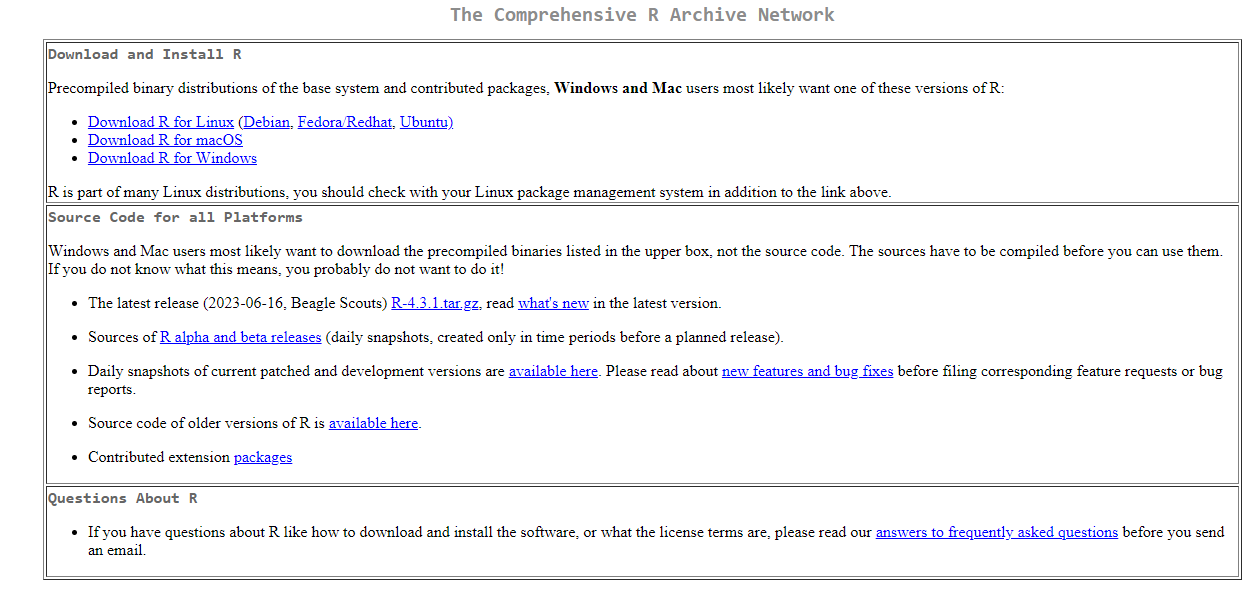
\includegraphics[width=6.91667in,height=4.11458in]{images/R download.PNG}
\item
  İndirilen sayfada \textbf{``base''} sekmesine tıklayın.

  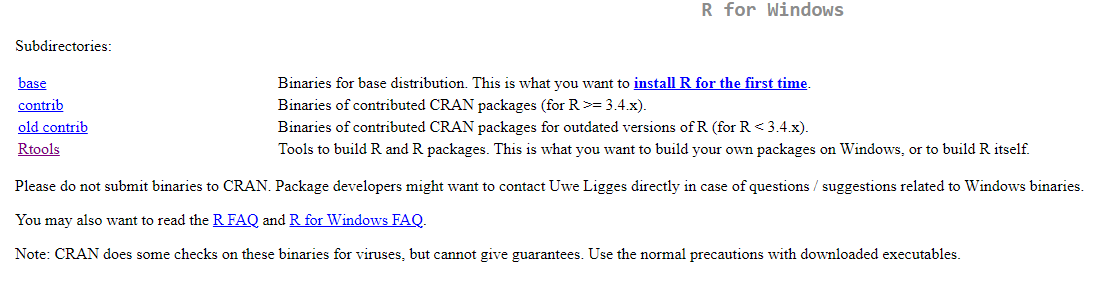
\includegraphics[width=6.90625in,height=2.79167in]{images/R download base.PNG}
\item
  Açılan sayfada ``Download R 4.3.1 for Windows'' linkine tıklayın ve
  dosyayı indirin.

  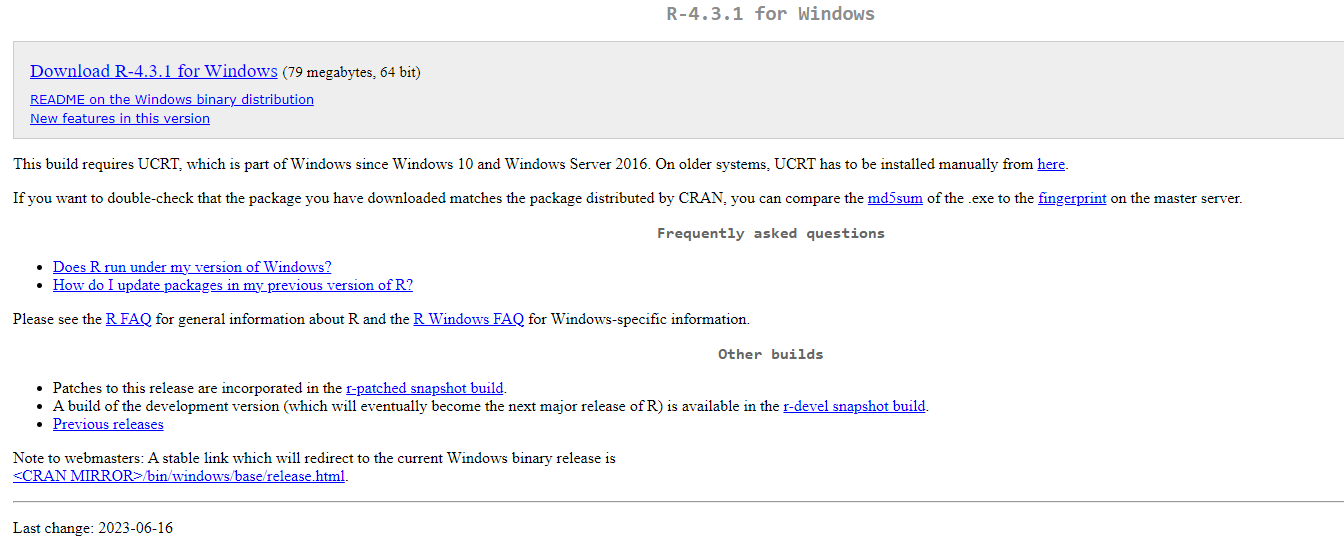
\includegraphics[width=6.8125in,height=3.5in]{images/R download win.PNG}

  \begin{tcolorbox}[enhanced jigsaw, colbacktitle=quarto-callout-warning-color!10!white, toprule=.15mm, breakable, titlerule=0mm, arc=.35mm, coltitle=black, colframe=quarto-callout-warning-color-frame, opacityback=0, bottomtitle=1mm, colback=white, toptitle=1mm, bottomrule=.15mm, rightrule=.15mm, left=2mm, title=\textcolor{quarto-callout-warning-color}{\faExclamationTriangle}\hspace{0.5em}{Dikkat}, leftrule=.75mm, opacitybacktitle=0.6]

  Sayfayı ziyaret ettiğiniz tarihlerde farklı sürümlerin olabileceğine
  dikkat edin. Örneğin ileri bir tarihte bu sayfayı ziyaret ettiğinizde
  R programının yeni sürümü ile karşılabilirsiniz. O yüzden sürüm
  bilgisi değişkenlik gösterebilir.

  \end{tcolorbox}
\item
  İndirilen dosyayı çift tıklayarak çalıştırın ve yükleyiciyi başlatın.
\item
  Yükleyici, R'nin temel sürümünü yüklemek için sizi yönlendirecektir.
  Varsayılan ayarları genellikle kabul edebilirsiniz.
\item
  Kurulum tamamlandığında, R'yi çalıştırmak için masaüstünüzde veya
  Başlat menüsünde \textbf{``R''} simgesini bulabilirsiniz.
\end{enumerate}

\textbf{Windows İşletim Sistemi İçin R Studio Kurulumu}

R editörü grafiksel bir arayüz olmayıp eski tip bir yazılım konsoludur.
\textbf{R Studio,} R programlama dili için geliştirilmiş entegre bir
geliştirme ortamı (IDE) ve arayüzüdür. R Studio, R kodlarını daha
verimli bir şekilde yazmanıza, çalıştırmanıza ve yönetmenize olanak
tanıyan daha modern ve kullanışlı bir arayüz sunmaktadır. Ayrıca veri
analizi, görselleştirme ve raporlama işlemleri için güçlü bir platform
sunar. R Studio, açık kaynak bir projedir ve ücretsiz olarak
kullanılabilir.

R Studio'nun kurulumu aşağıdaki adımlarla gerçekleştirilebilir:

\begin{enumerate}
\def\labelenumi{\arabic{enumi}.}
\item
  R Studio'nun en son sürümünü indirmek için aşağıdaki bağlantıyı
  kullanın:
  \href{https://www.rstudio.com/products/rstudio/download/}{\textbf{https://www.rstudio.com/products/rstudio/download/}}
\item
  Sayfada \textbf{``Download RStudio Desktop for Windows''} kısmına
  tıklayın ve indirmeyi başlatın.

  
\includegraphics[width=6.625in,height=4.02083in]{images/R Studio.PNG}
\item
  İndirilen dosyayı çift tıklayarak çalıştırın ve kurulumu başlatın.
  Kurulum sırasında varsayılan ayarları genellikle kabul edebilirsiniz.
\item
  Kurulum tamamlandığında, R Studio'yu başlatmak için masaüstünüzde veya
  Başlat menüsünde \textbf{``RStudio''} simgesini bulabilirsiniz.
\end{enumerate}

\hypertarget{r-studio-kiux15fiselleux15ftirme}{%
\section*{R Studio
Kişiselleştirme}\label{r-studio-kiux15fiselleux15ftirme}}
\addcontentsline{toc}{section}{R Studio Kişiselleştirme}

\markright{R Studio Kişiselleştirme}

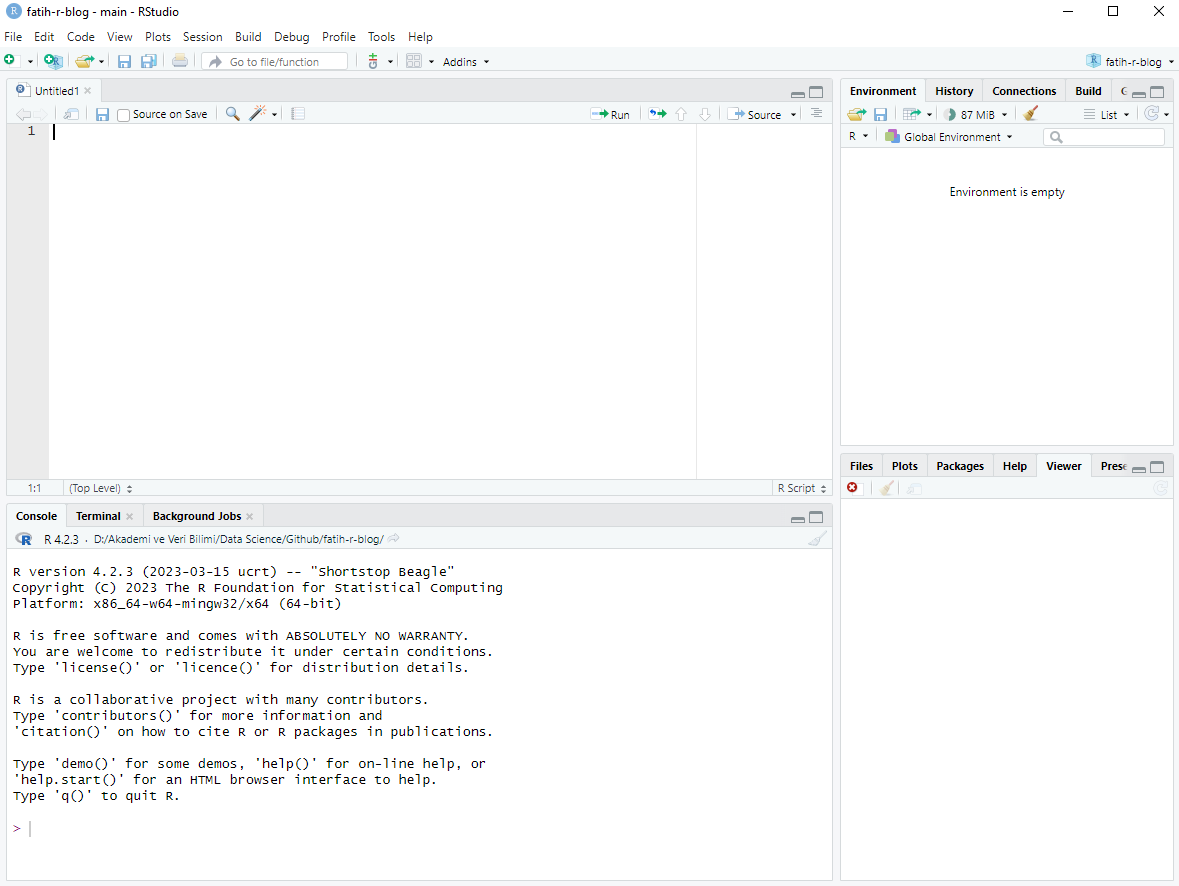
\includegraphics{images/RStudio.PNG}

RStudio, kullanıcıların ihtiyaçlarına göre kişiselleştirilebilen bir
entegre geliştirme ortamı (IDE) sunar. RStudio'yu kişiselleştirmek için
aşağıdaki yolları kullanabilirsiniz:

\begin{enumerate}
\def\labelenumi{\arabic{enumi}.}
\item
  \textbf{R Studio Arayüzündeki Alanları Değiştirme}: Resimde görüldüğü
  gibi yeni bir R Script açıldığı takdirde arayüzde 4 farklı alan
  görülmektedir. Bu alanlar isteğe göre yer değiştirilebilmektedir.
  Bunun için \textbf{``Tools''} (Araçlar) menüsünden \textbf{``Global
  Options''} (Genel Ayarlar) sekmesi açılır. Buradan \textbf{``Pane
  Layout''} kısmından istenilen ayarlar yapılabilir.
\item
  \textbf{Temayı ve Editör Stilini Değiştirme}: RStudio'nun görünümünü
  değiştirmek için birçok tema ve editör stilini seçebilirsiniz. Bu,
  yazılım geliştirme ortamınızın daha hoş veya kullanışlı olmasını
  sağlar. \textbf{``Tools''} (Araçlar) menüsünden \textbf{``Global
  Options''} (Genel Ayarlar) sekmesini seçerek bu ayarları
  değiştirebilirsiniz.
\item
  \textbf{Klavye Kısayollarını Kişiselleştirme}: RStudio'da kullanılan
  klavye kısayollarını özelleştirebilirsiniz. ``Tools'' (Araçlar)
  menüsünden ``Modify Keyboard Shortcuts'' (Klavye Kısayollarını
  Düzenle) seçeneğini kullanarak klavye kısayollarını tanımlayabilir
  veya değiştirebilirsiniz.
\item
  \textbf{Eklentileri ve Paketleri Kullanma}: RStudio, kullanıcıların
  işlevselliği genişletmek için eklentileri ve R paketlerini
  kullanmalarını sağlar. Bu paketler, kod otomatik tamamlama, kod
  görselleştirme, proje yönetimi gibi birçok işlemi kolaylaştırabilir. R
  Studio'nun sol üst köşesindeki \textbf{``Tools''} (Araçlar) menüsünden
  \textbf{``Install Packages''} (Paketleri Yükle) seçeneği ile yeni
  paketleri yükleyebilirsiniz.
\item
  \textbf{R Markdown Belgelerini Özelleştirme}: R Markdown belgeleri,
  raporlar ve belgeler oluşturmak için kullanılır. Bu belgeleri
  kişiselleştirebilirsiniz. R Markdown belgelerinin başlık, stil, tablo
  düzeni ve grafikler gibi birçok yönünü özelleştirebilirsiniz.
\item
  \textbf{Proje Ayarlarını Yapılandırma}: RStudio'da projeler kullanmak,
  projelerinizi daha düzenli ve etkili bir şekilde yönetmenize yardımcı
  olabilir. ``File'' (Dosya) menüsünden ``New Project'' (Yeni Proje)
  seçeneği ile yeni projeler oluşturabilir ve projelerinizi
  kişiselleştirebilirsiniz.
\item
  \textbf{Kod Tarayıcı ve Çalışma Ortamını Özelleştirme}: RStudio'nun
  sağ tarafında bulunan \textbf{``Environment''} (Çalışma Ortamı) ve
  \textbf{``Files''} (Dosyalar) sekmelerini özelleştirebilirsiniz. Bu
  sekmeleri dilediğiniz gibi düzenleyebilirsiniz.
\item
  \textbf{Addins Kullanma}: RStudio'nun ``Addins'' (Eklentiler) menüsü,
  kullanıcıların özel işlevleri ekleyebileceği bir bölümdür. Bu sayede
  belirli işlemleri hızlıca gerçekleştirebilirsiniz.
\end{enumerate}

RStudio'nun bu kişiselleştirme seçenekleri, kullanıcıların kendi
ihtiyaçlarına ve tercihlerine göre IDE'yi özelleştirmelerine olanak
tanır. Bu şekilde, RStudio'yu daha verimli ve kişiselleştirilmiş bir
şekilde kullanabilirsiniz. RStudio'nun ana bileşenleri ve temel
özellikleri ise şunlardır:

\begin{enumerate}
\def\labelenumi{\arabic{enumi}.}
\item
  \textbf{Script Editörü}: RStudio'nun sol üst kısmında yer alan bu
  bölüm, R kodlarını yazmak, düzenlemek ve çalıştırmak için kullanılır.
  Renk vurguları, otomatik tamamlama ve hata işaretleme gibi birçok
  yazılım geliştirme özelliği içerir.
\item
  \textbf{Environment (Çalışma Ortamı)} : Sağ üst köşede bulunan
  ``Çalışma Ortamı'' sekmesi, çalışan nesneleri ve değişkenleri
  görüntülemenizi sağlar. ``Files'' sekmesi ise projenizdeki dosyaları
  ve klasörleri görüntülemenize yardımcı olur.
\item
  \textbf{Console}: Alt sol köşede bulunan bu bölüm, R kodlarını anlık
  olarak çalıştırmanıza ve sonuçları görmesinize olanak tanır. R
  komutlarını doğrudan konsola yazabilir ve çalıştırabilirsiniz.
\item
  \textbf{Diğer Sekmeler} : RStudio, çeşitli grafikler ve
  görselleştirmeler oluşturmanıza olanak tanır. R koduyla çizilen
  grafikler, ``\textbf{Plots}'' sekmesinde görüntülenir. Bunu yanısıra
  ``\textbf{Help''} kısmında fonksiyonlar ile ilgili bilgi
  alınabilir,''\textbf{Packages''} kısmından ise paket yükleme vb. işler
  yapılabilir.
\end{enumerate}

\part{R Programlamaya Giriş}

R kodunun çalıştırılması oldukça basittir ve R Studio gibi entegre
geliştirme ortamları (IDE'ler) kullanırken daha da kolaylaşır. R kodunu
çalıştırmak için temel adımlar:

\begin{enumerate}
\def\labelenumi{\arabic{enumi}.}
\item
  \textbf{R Studio'yu Açın}: İlk adım, R Studio veya başka bir R
  IDE'sini açmaktır.
\item
  \textbf{Yeni Bir script uluşturun veya mevcut bir script kullanın}:

  \begin{itemize}
  \item
    R Studio'da, sol üst köşede bulunan ``File'' (Dosya) menüsünden
    ``New Script''seçeneği ile yeni bir R scripti oluşturabilirsiniz.
  \item
    Mevcut bir scripte gitmek istiyorsanız, ``File'' menüsünden ``Open
    Script'' seçeneğini kullanabilirsiniz.
  \end{itemize}
\item
  \textbf{R Kodunu Scripte Yazın}: Oluşturduğunuz veya açtığınız R
  skriptinde, R kodlarını yazın veya yapıştırın. Örneğin, basit bir
  hesaplama yapmak için aşağıdaki kodu kullanabilirsiniz:

\begin{Shaded}
\begin{Highlighting}[]
\NormalTok{x }\OtherTok{\textless{}{-}} \DecValTok{5}
\NormalTok{y }\OtherTok{\textless{}{-}} \DecValTok{10}
\NormalTok{z }\OtherTok{\textless{}{-}}\NormalTok{ x }\SpecialCharTok{+}\NormalTok{ y}
\NormalTok{z}
\end{Highlighting}
\end{Shaded}

\begin{verbatim}
[1] 15
\end{verbatim}
\item
  \textbf{Kodu Çalıştırma}:

  \begin{itemize}
  \item
    Çalıştırmak istediğiniz kodu seçin veya imleci çalıştırmak
    istediğiniz satıra getirin.
  \item
    Çalıştırma işlemi için aşağıdaki yöntemlerden birini
    kullanabilirsiniz:

    \begin{itemize}
    \item
      Klavyede varsayılan olarak ``Ctrl+Enter'' (Windows/Linux) veya
      ``Command+Enter'' (Mac) tuş kombinasyonunu kullanabilirsiniz.
    \item
      R Studio'daki ``Run'' (Çalıştır) düğmesini veya ``Run'' (Çalıştır)
      menüsünü kullanabilirsiniz.
    \item
      Çalıştırmak istediğiniz kodu seçtikten sonra sağ tıklarsanız,
      ``Run'' (Çalıştır) seçeneğini göreceksiniz.
    \end{itemize}
  \end{itemize}
\item
  \textbf{Sonuçları İnceleyin}: Çalıştırılan kodun sonuçları konsol
  penceresinde veya çıktı bölümünde görüntülenir. Örneğin, yukarıdaki
  örnekte ``z'' değişkeninin değeri olan ``15'' sonucunu göreceksiniz.
\end{enumerate}

\begin{tcolorbox}[enhanced jigsaw, colbacktitle=quarto-callout-warning-color!10!white, toprule=.15mm, breakable, titlerule=0mm, arc=.35mm, coltitle=black, colframe=quarto-callout-warning-color-frame, opacityback=0, bottomtitle=1mm, colback=white, toptitle=1mm, bottomrule=.15mm, rightrule=.15mm, left=2mm, title=\textcolor{quarto-callout-warning-color}{\faExclamationTriangle}\hspace{0.5em}{Dikkat}, leftrule=.75mm, opacitybacktitle=0.6]

Bir script üzerinden çalıştırılan R kodunun sonuçlarını sol alt kısımda
yer alan Console bölümünde görebilirsiniz. Aynı şekilde kodu Console
bölümüne yazıp Enter tuşuna bastığınızda yine sonuç alabilirsiniz. Ancak
script içerisinde yazılan kodları bir \textbf{\texttt{.R}} uzantılı
dosya olarak saklama ve daha sonradan bu dosyaya ulaşma şansınız varken,
Console ile çalıştırılan kodları bir \textbf{\texttt{.R}} dosyası olarak
saklama şansınız yoktur. Console tarafındaki sonuçlar geçici olarak
ekranda kalır ve R Studio'yu kapatıp açtığınızda tekrar yazdığınız ve
çalıştırdığınız kodlara ulaşamayabilirsiniz.

\end{tcolorbox}

\begin{tcolorbox}[enhanced jigsaw, colbacktitle=quarto-callout-tip-color!10!white, toprule=.15mm, breakable, titlerule=0mm, arc=.35mm, coltitle=black, colframe=quarto-callout-tip-color-frame, opacityback=0, bottomtitle=1mm, colback=white, toptitle=1mm, bottomrule=.15mm, rightrule=.15mm, left=2mm, title=\textcolor{quarto-callout-tip-color}{\faLightbulb}\hspace{0.5em}{İpucu}, leftrule=.75mm, opacitybacktitle=0.6]

Console tarafına yansıyan kodların ve sonuçların farklı formatlarda
saklama şansımız vardır. Bunun için \texttt{sink} fonksiyonunu
araştırmanızı önerebilirim.

\end{tcolorbox}

\hypertarget{temel-fonksiyonlar}{%
\chapter{Temel Fonksiyonlar}\label{temel-fonksiyonlar}}

\hypertarget{uxe7alux131ux15fma-dizini}{%
\section{Çalışma Dizini}\label{uxe7alux131ux15fma-dizini}}

Çalışma Dizini, üzerinde çalıştığınız veri kümeleri vb. gibi tüm gerekli
dosya ve belgelerinizi içeren yerdir. Çalışma dizininizi ayarlamanın iki
yolu vardır. İlk yol \ul{\textbf{getwd ve setwd}} işlevlerini
kullanmaktır. Diğer yol ise RStudio üzerinden
\ul{\textbf{Session\textgreater Set Working Directory}} youluyla
yapılabilir.

\begin{Shaded}
\begin{Highlighting}[]
\FunctionTok{getwd}\NormalTok{()}
\end{Highlighting}
\end{Shaded}

\begin{verbatim}
[1] "D:/Akademi ve Veri Bilimi/Data Science/Github/r-book-tr"
\end{verbatim}

\begin{itemize}
\item
  \ul{\textbf{\texttt{dir}}} veya \ul{\textbf{\texttt{list.files}}}
  komutları ile dizinde yer alan dosyalar öğrenilebilir.
\item
  \ul{\textbf{\texttt{dir.create}}} komutu ile yeni bir klasör
  oluşturmak mümkündür.
\item
  \ul{\textbf{\texttt{file.exists}}} kullanılarak klasörün var olup
  olmadığı sorgulanabilir.
\end{itemize}

\hypertarget{yardux131mcux131-bilgiler}{%
\section{Yardımcı Bilgiler}\label{yardux131mcux131-bilgiler}}

\textbf{R} komutlarında \emph{Büyük-küçük harf duyarlılığı (case
sensitive)} vardır.

\begin{Shaded}
\begin{Highlighting}[]
\NormalTok{a }\OtherTok{\textless{}{-}} \DecValTok{5}  
\FunctionTok{print}\NormalTok{(a)  }
\end{Highlighting}
\end{Shaded}

\begin{verbatim}
[1] 5
\end{verbatim}

\begin{Shaded}
\begin{Highlighting}[]
\NormalTok{A }\OtherTok{\textless{}{-}} \DecValTok{6}  
\FunctionTok{print}\NormalTok{(A) }
\end{Highlighting}
\end{Shaded}

\begin{verbatim}
[1] 6
\end{verbatim}

\textbf{Noktalı virgül (;)} işareti ile aynı satırda birden fazla kod
çalıştırılabilir hale getirilir.

\begin{Shaded}
\begin{Highlighting}[]
\NormalTok{x }\OtherTok{\textless{}{-}} \DecValTok{1}\NormalTok{ ; y }\OtherTok{\textless{}{-}} \DecValTok{2}\NormalTok{ ; z }\OtherTok{\textless{}{-}} \DecValTok{3}  
\NormalTok{x; y; z}
\end{Highlighting}
\end{Shaded}

\begin{verbatim}
[1] 1
\end{verbatim}

\begin{verbatim}
[1] 2
\end{verbatim}

\begin{verbatim}
[1] 3
\end{verbatim}

Komutlar arası açıklamaları ve yorumları \textbf{\#(hashtag)} ile
yazabiliriz. Hastagli satırlar, kod olarak algılanıp çalıştırılmaz. Bu
kısımlara yazılan kodlar ile ilgili hatırlatıcı bilgiler (comment)
yazılabilir.

\begin{Shaded}
\begin{Highlighting}[]
\CommentTok{\#6 ile başyalan ve  10 ile  biten tamsayıları c vektörüne atayalım  }
\NormalTok{c }\OtherTok{\textless{}{-}} \DecValTok{6}\SpecialCharTok{:}\DecValTok{10} 
\NormalTok{c}
\end{Highlighting}
\end{Shaded}

\begin{verbatim}
[1]  6  7  8  9 10
\end{verbatim}

\begin{itemize}
\item
  \textbf{\texttt{ls()}} çalışma alanındaki nesne ve fonksiyonları
  listeler.
\item
  \textbf{\texttt{rm(a)}} çalışma alanından \textbf{a} nesnesini siler.
\item
  \textbf{\texttt{rm(list=ls())}} bütün çalışma alanını temizler.
\item
  \textbf{\texttt{q()}} R'dan çıkış yapmayı sağlar.
\item
  \textbf{\texttt{install.packages("package")}} paket yüklemeyi sağlar.
\item
  \textbf{\texttt{library("package")}} yüklü olan paketi getirir.
\item
  \textbf{\texttt{installed.packages()}} yüklü olan paketleri listeler
\item
  \textbf{\texttt{options(digits=10)}} sayılarda ondalık kısmın basamak
  sayısını ifade eder.
\item
  \textbf{\texttt{help()}} fonksiyonu ya da \textbf{\texttt{?}} ile bir
  fonksiyon hakkında yardım alınabilir. Örneğin mean fonksiyonu ile
  ilgili yardım almak için scripte \texttt{?mean} ya da help(mean)
  yazmanız ve çalıştırmanız yeterlidir. Bunun yanı sıra R Studio
  penceresinin sağ alt kısmındaki help alanını kullanabilirsiniz.
\end{itemize}

\hypertarget{atama-operatuxf6ruxfc}{%
\section{Atama Operatörü}\label{atama-operatuxf6ruxfc}}

Bir değişkene, tabloya veya objeye değer atarken \textbf{`\textless-'}
veya \textbf{`='} operatörü kullanılır. `\textbf{\textless-}' atama
operatöründe ok hangi yöndeyse o tarafa atama yapılır. Genellikle
`\textbf{\textless-}' operatörü kullanılmaktadır. Çünkü `\textbf{=}'
operatörü filtrelemelerde veya işlemlerdeki `\textbf{==}' ile
karıştırılabilmektedir. Ayrıca fonksiyonlar içinde de kullanılabildiği
için kod karmaşasına sebebiyet verebilir. Her iki operatör de aynı
işlevi görmektedir.

\begin{Shaded}
\begin{Highlighting}[]
\CommentTok{\# a\textquotesingle{}ya 20 değerini atayalım  }
\NormalTok{a }\OtherTok{\textless{}{-}} \DecValTok{20}    
\CommentTok{\# tabloyu ya da değeri görüntülemek için nesnenin kendisi de direkt yazılabilir.  }
\CommentTok{\# ya da print fonksiyonu kullanılabilir.   }
\FunctionTok{print}\NormalTok{(a)    }
\end{Highlighting}
\end{Shaded}

\begin{verbatim}
[1] 20
\end{verbatim}

\begin{Shaded}
\begin{Highlighting}[]
\CommentTok{\# b\textquotesingle{}ye 12 değerini atayalım  }
\NormalTok{b }\OtherTok{\textless{}{-}} \DecValTok{12}  
\FunctionTok{print}\NormalTok{(b)   }
\end{Highlighting}
\end{Shaded}

\begin{verbatim}
[1] 12
\end{verbatim}

\begin{Shaded}
\begin{Highlighting}[]
\CommentTok{\# a ve b değerlerinden üretilen bir c değeri üretelim.   }
\NormalTok{c }\OtherTok{\textless{}{-}} \DecValTok{2} \SpecialCharTok{*}\NormalTok{ a }\SpecialCharTok{+} \DecValTok{3} \SpecialCharTok{*}\NormalTok{ b  }
\FunctionTok{print}\NormalTok{(c) }
\end{Highlighting}
\end{Shaded}

\begin{verbatim}
[1] 76
\end{verbatim}

\textbf{c()} ile vektör oluştutulabilir. c ``combine'' (birleştirmek)
kelimesinin ilk harfini ifade eder. Bir değişkene birden fazla değer
atamak istediğimizde kullanılır.

\begin{Shaded}
\begin{Highlighting}[]
\CommentTok{\# d adında bir vektör oluşturalım ve değerler atayalım.   }
\NormalTok{d }\OtherTok{\textless{}{-}} \FunctionTok{c}\NormalTok{(}\DecValTok{4}\NormalTok{,}\DecValTok{7}\NormalTok{,}\DecValTok{13}\NormalTok{)  }
\NormalTok{d }
\end{Highlighting}
\end{Shaded}

\begin{verbatim}
[1]  4  7 13
\end{verbatim}

Bir metini değişkene atamak istersek de aşağıdaki gibi metin ``\,''
işareti içine yazılmalıdır.

\begin{Shaded}
\begin{Highlighting}[]
\NormalTok{metin }\OtherTok{\textless{}{-}} \StringTok{"Merhaba Arkadaşlar"}  
\FunctionTok{print}\NormalTok{(metin)}
\end{Highlighting}
\end{Shaded}

\begin{verbatim}
[1] "Merhaba Arkadaşlar"
\end{verbatim}

\hypertarget{matematiksel-operatuxf6rler}{%
\section{Matematiksel Operatörler}\label{matematiksel-operatuxf6rler}}

R ve R Studio, güçlü bir hesap makinesi olarak kabul edilebilir.

\begin{Shaded}
\begin{Highlighting}[]
\DecValTok{3}\SpecialCharTok{+}\DecValTok{5} 
\end{Highlighting}
\end{Shaded}

\begin{verbatim}
[1] 8
\end{verbatim}

\begin{Shaded}
\begin{Highlighting}[]
\DecValTok{7}\SpecialCharTok{*}\DecValTok{8} 
\end{Highlighting}
\end{Shaded}

\begin{verbatim}
[1] 56
\end{verbatim}

\begin{Shaded}
\begin{Highlighting}[]
\DecValTok{88}\SpecialCharTok{/}\DecValTok{2} 
\end{Highlighting}
\end{Shaded}

\begin{verbatim}
[1] 44
\end{verbatim}

\begin{Shaded}
\begin{Highlighting}[]
\DecValTok{3}\SpecialCharTok{*}\NormalTok{(}\DecValTok{12}\SpecialCharTok{+}\NormalTok{(}\DecValTok{15}\SpecialCharTok{/}\DecValTok{3{-}2}\NormalTok{)) }
\end{Highlighting}
\end{Shaded}

\begin{verbatim}
[1] 45
\end{verbatim}

\begin{Shaded}
\begin{Highlighting}[]
\DecValTok{9}\SpecialCharTok{\^{}}\DecValTok{2} \CommentTok{\# karesini alır }
\end{Highlighting}
\end{Shaded}

\begin{verbatim}
[1] 81
\end{verbatim}

\begin{Shaded}
\begin{Highlighting}[]
\NormalTok{a }\OtherTok{\textless{}{-}}  \DecValTok{3} 
\NormalTok{b }\OtherTok{\textless{}{-}}\NormalTok{  a}\SpecialCharTok{\^{}}\DecValTok{2} 
\FunctionTok{print}\NormalTok{(b) }
\end{Highlighting}
\end{Shaded}

\begin{verbatim}
[1] 9
\end{verbatim}

\begin{Shaded}
\begin{Highlighting}[]
\FunctionTok{log}\NormalTok{(}\DecValTok{15}\NormalTok{) }\CommentTok{\#ln15 yani doğal logaritma }
\end{Highlighting}
\end{Shaded}

\begin{verbatim}
[1] 2.70805
\end{verbatim}

\begin{Shaded}
\begin{Highlighting}[]
\FunctionTok{log10}\NormalTok{(}\DecValTok{1000}\NormalTok{) }\CommentTok{\# 10 tabanına göre hesaplama }
\end{Highlighting}
\end{Shaded}

\begin{verbatim}
[1] 3
\end{verbatim}

\begin{Shaded}
\begin{Highlighting}[]
\FunctionTok{exp}\NormalTok{(}\DecValTok{12}\NormalTok{) }\CommentTok{\#exponential power of the number. e (2.718) üzeri 12 }
\end{Highlighting}
\end{Shaded}

\begin{verbatim}
[1] 162754.8
\end{verbatim}

\begin{Shaded}
\begin{Highlighting}[]
\FunctionTok{factorial}\NormalTok{(}\DecValTok{6}\NormalTok{) }\CommentTok{\# faktöriyel hesaplama yapar }
\end{Highlighting}
\end{Shaded}

\begin{verbatim}
[1] 720
\end{verbatim}

\begin{Shaded}
\begin{Highlighting}[]
\FunctionTok{sqrt}\NormalTok{(}\DecValTok{81}\NormalTok{) }\CommentTok{\# karekök alma }
\end{Highlighting}
\end{Shaded}

\begin{verbatim}
[1] 9
\end{verbatim}

\begin{Shaded}
\begin{Highlighting}[]
\FunctionTok{abs}\NormalTok{(}\SpecialCharTok{{-}}\DecValTok{3}\NormalTok{) }\CommentTok{\# mutlak değer }
\end{Highlighting}
\end{Shaded}

\begin{verbatim}
[1] 3
\end{verbatim}

\begin{Shaded}
\begin{Highlighting}[]
\FunctionTok{sign}\NormalTok{(}\SpecialCharTok{{-}}\DecValTok{5}\NormalTok{) }\CommentTok{\# işaret bulma }
\end{Highlighting}
\end{Shaded}

\begin{verbatim}
[1] -1
\end{verbatim}

\begin{Shaded}
\begin{Highlighting}[]
\FunctionTok{sin}\NormalTok{(}\DecValTok{45}\NormalTok{) }\CommentTok{\# sinüs }
\end{Highlighting}
\end{Shaded}

\begin{verbatim}
[1] 0.8509035
\end{verbatim}

\begin{Shaded}
\begin{Highlighting}[]
\FunctionTok{cos}\NormalTok{(}\DecValTok{90}\NormalTok{) }\CommentTok{\# cosinüs }
\end{Highlighting}
\end{Shaded}

\begin{verbatim}
[1] -0.4480736
\end{verbatim}

\begin{Shaded}
\begin{Highlighting}[]
\NormalTok{pi }\CommentTok{\# pi sayısı }
\end{Highlighting}
\end{Shaded}

\begin{verbatim}
[1] 3.141593
\end{verbatim}

\begin{Shaded}
\begin{Highlighting}[]
\FunctionTok{tan}\NormalTok{(pi) }\CommentTok{\# tanjant}
\end{Highlighting}
\end{Shaded}

\begin{verbatim}
[1] -1.224647e-16
\end{verbatim}

\hypertarget{mantux131ksal-operatuxf6rler}{%
\section{Mantıksal Operatörler}\label{mantux131ksal-operatuxf6rler}}

Mantıksal sorgulamalar, koşullarda ve filtrelerde kullanılmaktadır.
Verilen koşul veya filtre sağlandığında \textbf{TRUE}, sağlanmadığında
ise \textbf{FALSE} değerleri elde edilmektedir. Bu mantıksal operatörler
ayrıca komutlar içindeki özellikleri aktifleştirmek ve pasifleştirmek
için de kullanılmaktadır.

Mantıksal operatörler aşağıdaki şekilde kullanılmaktadır:

\begin{itemize}
\item
  eşittir : \textbf{==}
\item
  eşit değildir : \textbf{!=}
\item
  küçüktür : \textbf{\textless{}}
\item
  küçük eşittir : \textbf{\textless=}
\item
  büyüktür : \textbf{\textgreater{}}
\item
  büyük eşittir : \textbf{\textgreater=}
\item
  x değil : \textbf{!x}
\item
  x ve y : \textbf{x\&y}
\item
  x veya y: \textbf{x\textbar y}
\end{itemize}

\begin{Shaded}
\begin{Highlighting}[]
\DecValTok{3} \SpecialCharTok{\textgreater{}} \DecValTok{5}
\end{Highlighting}
\end{Shaded}

\begin{verbatim}
[1] FALSE
\end{verbatim}

\begin{Shaded}
\begin{Highlighting}[]
\CommentTok{\# \& (ve) operatörü}
\CommentTok{\# iki durumda TRUE ise sonuç TRUE döner.}
\DecValTok{3} \SpecialCharTok{\textless{}} \DecValTok{5} \SpecialCharTok{\&} \DecValTok{8} \SpecialCharTok{\textgreater{}} \DecValTok{7}
\end{Highlighting}
\end{Shaded}

\begin{verbatim}
[1] TRUE
\end{verbatim}

\begin{Shaded}
\begin{Highlighting}[]
\CommentTok{\# bir durum FALSE diğer durum TRUE ise sonuç FALSE döner.}
\DecValTok{3} \SpecialCharTok{\textless{}} \DecValTok{5} \SpecialCharTok{\&} \DecValTok{6} \SpecialCharTok{\textgreater{}} \DecValTok{7}
\end{Highlighting}
\end{Shaded}

\begin{verbatim}
[1] FALSE
\end{verbatim}

\begin{Shaded}
\begin{Highlighting}[]
\CommentTok{\# iki durumda FALSE ise sonuç FALSE döner.}
\DecValTok{6} \SpecialCharTok{\textless{}} \DecValTok{5} \SpecialCharTok{\&} \DecValTok{6} \SpecialCharTok{\textgreater{}} \DecValTok{7}
\end{Highlighting}
\end{Shaded}

\begin{verbatim}
[1] FALSE
\end{verbatim}

\begin{Shaded}
\begin{Highlighting}[]
\CommentTok{\# | (veya) operatörü}
\CommentTok{\# Her iki durumdan birisi TRUE ise TRUE döner}
\NormalTok{(}\DecValTok{5}\SpecialCharTok{==}\DecValTok{4}\NormalTok{) }\SpecialCharTok{|}\NormalTok{ (}\DecValTok{3}\SpecialCharTok{!=}\DecValTok{4}\NormalTok{)}
\end{Highlighting}
\end{Shaded}

\begin{verbatim}
[1] TRUE
\end{verbatim}

\hypertarget{veri-tipleri-ve-yapux131larux131}{%
\chapter{Veri Tipleri ve
Yapıları}\label{veri-tipleri-ve-yapux131larux131}}

\hypertarget{veri-tipleri}{%
\section{Veri Tipleri}\label{veri-tipleri}}

R'da kulllanılan 5 temel veri tipi vardır. Bu veri tipleri atomic
vectörler olarak da bilinir. Atomic olması vektörlerin homojen olması
anlamına gelmektedir. Yani vektör içerisinde aynı veri tipinden değerler
yer alabilir. Veri tipleri;

\begin{itemize}
\item
  numeric veya double (reel sayılar)
\item
  integer (tamsayılar)
\item
  complex (karmaşık sayılar)
\item
  character (metinsel ifadeler)
\item
  logical, TRUE ve FALSE (mantıksal)
\end{itemize}

\texttt{typeof()} veya \texttt{class()} fonksiyonları ile veri tipi
öğrenilebilir.

\begin{tcolorbox}[enhanced jigsaw, colbacktitle=quarto-callout-important-color!10!white, toprule=.15mm, breakable, titlerule=0mm, arc=.35mm, coltitle=black, colframe=quarto-callout-important-color-frame, opacityback=0, bottomtitle=1mm, colback=white, toptitle=1mm, bottomrule=.15mm, rightrule=.15mm, left=2mm, title=\textcolor{quarto-callout-important-color}{\faExclamation}\hspace{0.5em}{Önemli}, leftrule=.75mm, opacitybacktitle=0.6]

\textbf{\texttt{typeof()}} ve \textbf{\texttt{class()}} fonksiyonları, R
programlama dilinde nesnelerin özelliklerini sorgulamak için kullanılır.
Farklı amaçlara hizmet ederler ve bazı durumlarda farklı sonuçlar
üretebilirler.

\begin{itemize}
\item
  \textbf{\texttt{typeof()}} fonksiyonu, bir nesnenin temel veri türünü
  belirler. Örneğin, bir nesnenin karakter dizisi (string), sayı, liste,
  fonksiyon veya vektör gibi temel veri türlerinden hangisine ait
  olduğunu gösterir. Ancak, nesnenin özel sınıfını (class) ifade etmez.
  Örneğin, bir faktörün \textbf{\texttt{typeof()}} değeri ``integer''
  olabilir.
\item
  \textbf{\texttt{class()}} fonksiyonu ise bir nesnenin özel sınıfını
  belirtir. Eğer bir nesne özel bir sınıfa aitse (örneğin, bir veri
  çerçevesi veya faktör), \textbf{\texttt{class()}} fonksiyonu bu özel
  sınıfın adını verir. Eğer nesne birden fazla sınıfa aitse, sınıflar
  bir sıra halinde listelenir.
\end{itemize}

Bu fonksiyonlar genellikle birlikte kullanılır çünkü bir nesnenin veri
tipi ve sınıfı arasında farklılıklar olabilir. Örneğin, bir veri
çerçevesi \textbf{\texttt{typeof()}} ile incelendiğinde
\textbf{\texttt{list}} çıkabilir, çünkü veri çerçeveleri bir liste
türündedir. Ancak, \textbf{\texttt{class()}} fonksiyonu bu nesnenin özel
sınıfını, yani \textbf{\texttt{data.frame}} olarak gösterecektir. Bu
farklılıklar, bir nesnenin hangi özelliklere sahip olduğunu daha iyi
anlamak için kullanılabilir.

\end{tcolorbox}

\textbf{numeric}

\begin{Shaded}
\begin{Highlighting}[]
\NormalTok{a }\OtherTok{\textless{}{-}} \FloatTok{3.5}
\FunctionTok{class}\NormalTok{(a)}
\end{Highlighting}
\end{Shaded}

\begin{verbatim}
[1] "numeric"
\end{verbatim}

\begin{Shaded}
\begin{Highlighting}[]
\FunctionTok{typeof}\NormalTok{(a) }\CommentTok{\# typeof numeriklerin tipini double olarak gösterir.}
\end{Highlighting}
\end{Shaded}

\begin{verbatim}
[1] "double"
\end{verbatim}

\begin{Shaded}
\begin{Highlighting}[]
\FunctionTok{is.numeric}\NormalTok{(a) }\CommentTok{\# verinin tipinin numerik olup olmadığı sorgulanır.}
\end{Highlighting}
\end{Shaded}

\begin{verbatim}
[1] TRUE
\end{verbatim}

\textbf{integer}

\begin{Shaded}
\begin{Highlighting}[]
\NormalTok{b }\OtherTok{\textless{}{-}} \DecValTok{5}
\FunctionTok{class}\NormalTok{(b)}
\end{Highlighting}
\end{Shaded}

\begin{verbatim}
[1] "numeric"
\end{verbatim}

\begin{Shaded}
\begin{Highlighting}[]
\FunctionTok{is.integer}\NormalTok{(b)}
\end{Highlighting}
\end{Shaded}

\begin{verbatim}
[1] FALSE
\end{verbatim}

\begin{Shaded}
\begin{Highlighting}[]
\NormalTok{c }\OtherTok{\textless{}{-}}\NormalTok{ 6L }\CommentTok{\# integer olması için sayının sağına L yazılır.}
\FunctionTok{class}\NormalTok{(c)}
\end{Highlighting}
\end{Shaded}

\begin{verbatim}
[1] "integer"
\end{verbatim}

\begin{Shaded}
\begin{Highlighting}[]
\FunctionTok{is.integer}\NormalTok{(c)}
\end{Highlighting}
\end{Shaded}

\begin{verbatim}
[1] TRUE
\end{verbatim}

\begin{Shaded}
\begin{Highlighting}[]
\FunctionTok{class}\NormalTok{(}\FunctionTok{as.integer}\NormalTok{(b)) }\CommentTok{\# as. ile baslayan fonksiyonlar dönüşüm için kullanılır.}
\end{Highlighting}
\end{Shaded}

\begin{verbatim}
[1] "integer"
\end{verbatim}

\textbf{complex}

\begin{Shaded}
\begin{Highlighting}[]
\NormalTok{z }\OtherTok{\textless{}{-}} \DecValTok{4} \SpecialCharTok{+}\NormalTok{ 2i}
\FunctionTok{class}\NormalTok{(z)}
\end{Highlighting}
\end{Shaded}

\begin{verbatim}
[1] "complex"
\end{verbatim}

\textbf{character}

\begin{Shaded}
\begin{Highlighting}[]
\NormalTok{d }\OtherTok{\textless{}{-}} \StringTok{"R Programlama"}
\FunctionTok{class}\NormalTok{(d)}
\end{Highlighting}
\end{Shaded}

\begin{verbatim}
[1] "character"
\end{verbatim}

\begin{Shaded}
\begin{Highlighting}[]
\NormalTok{e }\OtherTok{\textless{}{-}} \StringTok{"5.5"}
\FunctionTok{class}\NormalTok{(e)}
\end{Highlighting}
\end{Shaded}

\begin{verbatim}
[1] "character"
\end{verbatim}

\begin{Shaded}
\begin{Highlighting}[]
\FunctionTok{class}\NormalTok{(}\FunctionTok{as.numeric}\NormalTok{(e))}
\end{Highlighting}
\end{Shaded}

\begin{verbatim}
[1] "numeric"
\end{verbatim}

\textbf{logical}

\begin{Shaded}
\begin{Highlighting}[]
\NormalTok{x }\OtherTok{\textless{}{-}} \ConstantTok{TRUE}
\NormalTok{y }\OtherTok{\textless{}{-}} \ConstantTok{FALSE}
\FunctionTok{class}\NormalTok{(}\FunctionTok{c}\NormalTok{(x,y))}
\end{Highlighting}
\end{Shaded}

\begin{verbatim}
[1] "logical"
\end{verbatim}

\begin{Shaded}
\begin{Highlighting}[]
\FunctionTok{as.integer}\NormalTok{(}\FunctionTok{c}\NormalTok{(x,y)) }\CommentTok{\# TRUE ve FALSE numeric olarak 1 ve 0 değerine karşılık gelir.}
\end{Highlighting}
\end{Shaded}

\begin{verbatim}
[1] 1 0
\end{verbatim}

\hypertarget{veri-yapux131larux131}{%
\section{Veri Yapıları}\label{veri-yapux131larux131}}

\begin{figure}

{\centering 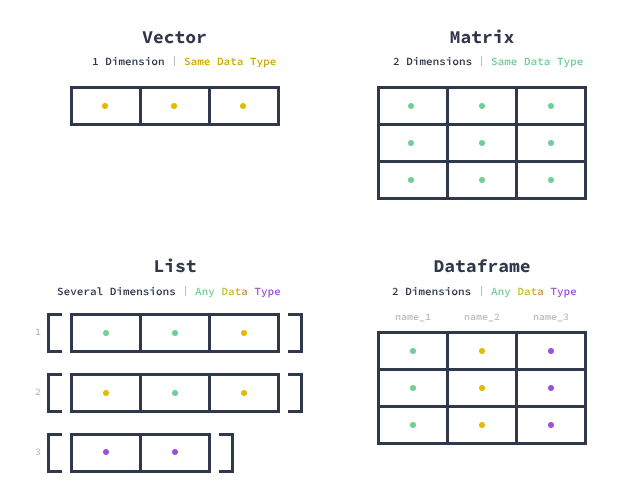
\includegraphics{images/data_structures.png}

}

\caption{https://app.dataquest.io/m/493/dataframes-in-r/1/introduction}

\end{figure}

\hypertarget{vektuxf6rler}{%
\subsection{Vektörler}\label{vektuxf6rler}}

\begin{itemize}
\item
  R'daki en temel nesneler vektörlerdir.
\item
  Vektörler homojen yapıya sahiptir yani bütün elemanları aynı veri
  tipinde olmalıdır.
\item
  Vektörler tek boyutludur.
\item
  Bir vektör oluşturmak için kullanabilecek en temel fonksiyon
  \textbf{\texttt{c()}}'dir.
\end{itemize}

\begin{Shaded}
\begin{Highlighting}[]
\NormalTok{v }\OtherTok{\textless{}{-}} \FunctionTok{c}\NormalTok{(}\DecValTok{1}\NormalTok{,}\DecValTok{4}\NormalTok{,}\DecValTok{7}\NormalTok{,}\DecValTok{2}\NormalTok{,}\DecValTok{5}\NormalTok{,}\DecValTok{8}\NormalTok{,}\DecValTok{3}\NormalTok{,}\DecValTok{6}\NormalTok{,}\DecValTok{9}\NormalTok{)}

\NormalTok{v[}\DecValTok{1}\NormalTok{] }\CommentTok{\# 1. elemanını seçer}
\end{Highlighting}
\end{Shaded}

\begin{verbatim}
[1] 1
\end{verbatim}

\begin{Shaded}
\begin{Highlighting}[]
\NormalTok{v[}\DecValTok{3}\NormalTok{] }\CommentTok{\# 3. elemanını seçer}
\end{Highlighting}
\end{Shaded}

\begin{verbatim}
[1] 7
\end{verbatim}

\begin{Shaded}
\begin{Highlighting}[]
\NormalTok{v[}\FunctionTok{c}\NormalTok{(}\DecValTok{3}\NormalTok{,}\DecValTok{7}\NormalTok{)] }\CommentTok{\# 3. ve 7. elemani secer}
\end{Highlighting}
\end{Shaded}

\begin{verbatim}
[1] 7 3
\end{verbatim}

\begin{Shaded}
\begin{Highlighting}[]
\NormalTok{v[}\DecValTok{1}\SpecialCharTok{:}\DecValTok{6}\NormalTok{] }\CommentTok{\# 1. elemandan 6. elemana kadar secer}
\end{Highlighting}
\end{Shaded}

\begin{verbatim}
[1] 1 4 7 2 5 8
\end{verbatim}

\begin{Shaded}
\begin{Highlighting}[]
\NormalTok{v[}\SpecialCharTok{{-}}\DecValTok{2}\NormalTok{] }\CommentTok{\# 2. elemani haric tutarak secer}
\end{Highlighting}
\end{Shaded}

\begin{verbatim}
[1] 1 7 2 5 8 3 6 9
\end{verbatim}

\begin{Shaded}
\begin{Highlighting}[]
\FunctionTok{length}\NormalTok{(v) }\CommentTok{\# vektörün uzunluğunu gösterir}
\end{Highlighting}
\end{Shaded}

\begin{verbatim}
[1] 9
\end{verbatim}

\begin{Shaded}
\begin{Highlighting}[]
\NormalTok{v2 }\OtherTok{\textless{}{-}} \FunctionTok{c}\NormalTok{(v,}\DecValTok{12}\NormalTok{) }\CommentTok{\# vektöre eleman ekleme}
\NormalTok{v2}
\end{Highlighting}
\end{Shaded}

\begin{verbatim}
 [1]  1  4  7  2  5  8  3  6  9 12
\end{verbatim}

\begin{Shaded}
\begin{Highlighting}[]
\CommentTok{\# : ile başlangıç ve bitiş değerleri belli olan vektörler yaratılabilir.}

\NormalTok{v3 }\OtherTok{\textless{}{-}} \DecValTok{1}\SpecialCharTok{:}\DecValTok{10}
\NormalTok{v3}
\end{Highlighting}
\end{Shaded}

\begin{verbatim}
 [1]  1  2  3  4  5  6  7  8  9 10
\end{verbatim}

\begin{Shaded}
\begin{Highlighting}[]
\NormalTok{v4 }\OtherTok{\textless{}{-}} \DecValTok{11}\SpecialCharTok{:}\DecValTok{20}
\NormalTok{v4}
\end{Highlighting}
\end{Shaded}

\begin{verbatim}
 [1] 11 12 13 14 15 16 17 18 19 20
\end{verbatim}

\begin{Shaded}
\begin{Highlighting}[]
\CommentTok{\# Vektörler ile matematiksel işlemler yapılabilir.}

\NormalTok{v3 }\SpecialCharTok{+}\NormalTok{ v4}
\end{Highlighting}
\end{Shaded}

\begin{verbatim}
 [1] 12 14 16 18 20 22 24 26 28 30
\end{verbatim}

\begin{Shaded}
\begin{Highlighting}[]
\NormalTok{v3 }\SpecialCharTok{/}\NormalTok{ v4}
\end{Highlighting}
\end{Shaded}

\begin{verbatim}
 [1] 0.09090909 0.16666667 0.23076923 0.28571429 0.33333333 0.37500000
 [7] 0.41176471 0.44444444 0.47368421 0.50000000
\end{verbatim}

\begin{Shaded}
\begin{Highlighting}[]
\DecValTok{2} \SpecialCharTok{*}\NormalTok{ v3 }\SpecialCharTok{{-}}\NormalTok{ v4}
\end{Highlighting}
\end{Shaded}

\begin{verbatim}
 [1] -9 -8 -7 -6 -5 -4 -3 -2 -1  0
\end{verbatim}

\hypertarget{vektuxf6rler-ile-kullanux131labilecek-bazux131-temel-fonksiyonlar}{%
\subsubsection{Vektörler İle Kullanılabilecek Bazı Temel
Fonksiyonlar}\label{vektuxf6rler-ile-kullanux131labilecek-bazux131-temel-fonksiyonlar}}

\textbf{seq()}

\textbf{\texttt{seq()}} fonksiyonu, ardışık sayı dizileri oluşturmak
için kullanılır. Bu fonksiyon, başlangıç ve bitiş değerlerinin yanı sıra
belirli bir artış veya azalış miktarını belirterek ardışık bir dizi
oluşturmanızı sağlar.

\textbf{\texttt{seq()}} fonksiyonu genellikle üç temel parametre alır:

\begin{enumerate}
\def\labelenumi{\arabic{enumi}.}
\item
  \textbf{\texttt{from}}: Dizinin başlangıç değeri.
\item
  \textbf{\texttt{to}}: Dizinin bitiş değeri.
\item
  \textbf{\texttt{by}}: Opsiyonel olarak belirlenebilen artış/azalış
  miktarı.
\end{enumerate}

\begin{Shaded}
\begin{Highlighting}[]
\FunctionTok{seq}\NormalTok{(}\AttributeTok{from =} \DecValTok{5}\NormalTok{, }\AttributeTok{to =} \DecValTok{50}\NormalTok{, }\AttributeTok{by =}\DecValTok{5}\NormalTok{) }\CommentTok{\# 5 ile başlayan 50 ile biten 5şer artan vektör}
\end{Highlighting}
\end{Shaded}

\begin{verbatim}
 [1]  5 10 15 20 25 30 35 40 45 50
\end{verbatim}

\begin{Shaded}
\begin{Highlighting}[]
\FunctionTok{seq}\NormalTok{(}\AttributeTok{from =} \DecValTok{5}\NormalTok{, }\AttributeTok{to =} \DecValTok{50}\NormalTok{, }\AttributeTok{length =} \DecValTok{7}\NormalTok{) }\CommentTok{\# 5 ile başlayan 50 ile 7 elemanlı vektör}
\end{Highlighting}
\end{Shaded}

\begin{verbatim}
[1]  5.0 12.5 20.0 27.5 35.0 42.5 50.0
\end{verbatim}

\begin{Shaded}
\begin{Highlighting}[]
\FunctionTok{seq}\NormalTok{(}\DecValTok{5}\NormalTok{,}\DecValTok{1}\NormalTok{,}\SpecialCharTok{{-}}\DecValTok{1}\NormalTok{) }\CommentTok{\# 5 ile baslayıp 1\textquotesingle{}e kadar 1\textquotesingle{}er azaltarak vektor olusturma}
\end{Highlighting}
\end{Shaded}

\begin{verbatim}
[1] 5 4 3 2 1
\end{verbatim}

\textbf{rep()}

\textbf{\texttt{rep()}} fonksiyonu, R programlama dilinde tekrarlanan
öğelerden oluşan vektörler oluşturmak için kullanılır. Bu fonksiyon,
belirli bir öğenin veya öğelerin tekrarlanarak bir vektör
oluşturulmasına izin verir.

\textbf{\texttt{rep()}} fonksiyonunun temel parametreleri şunlardır:

\begin{itemize}
\item
  \textbf{\texttt{x}}: Tekrarlanacak öğelerin kendisi veya vektörü.
\item
  \textbf{\texttt{times}}: Tekrar sayısını belirten bir sayı veya
  vektör.
\item
  \textbf{\texttt{each}}: Her bir öğenin kaç kez tekrarlanacağını
  belirten bir sayı veya vektör.
\item
  \textbf{\texttt{length.out:}} çıktının istenen uzunluğu
\end{itemize}

\begin{Shaded}
\begin{Highlighting}[]
\FunctionTok{rep}\NormalTok{(}\DecValTok{10}\NormalTok{,}\AttributeTok{times =} \DecValTok{8}\NormalTok{) }\CommentTok{\# 8 tane 10 değeri olan vektör}
\end{Highlighting}
\end{Shaded}

\begin{verbatim}
[1] 10 10 10 10 10 10 10 10
\end{verbatim}

\begin{Shaded}
\begin{Highlighting}[]
\FunctionTok{rep}\NormalTok{(}\FunctionTok{c}\NormalTok{(}\DecValTok{1}\NormalTok{,}\DecValTok{2}\NormalTok{,}\DecValTok{3}\NormalTok{), }\AttributeTok{times =} \DecValTok{4}\NormalTok{) }\CommentTok{\# 1,2,3 vektörünün 4 defa tekrarlanması}
\end{Highlighting}
\end{Shaded}

\begin{verbatim}
 [1] 1 2 3 1 2 3 1 2 3 1 2 3
\end{verbatim}

\begin{Shaded}
\begin{Highlighting}[]
\FunctionTok{rep}\NormalTok{(}\FunctionTok{c}\NormalTok{(}\DecValTok{1}\NormalTok{,}\DecValTok{2}\NormalTok{,}\DecValTok{3}\NormalTok{), }\AttributeTok{each =} \DecValTok{4}\NormalTok{) }\CommentTok{\# each argünmanı ile sıralı ve tekrarlı vektör}
\end{Highlighting}
\end{Shaded}

\begin{verbatim}
 [1] 1 1 1 1 2 2 2 2 3 3 3 3
\end{verbatim}

\begin{Shaded}
\begin{Highlighting}[]
\FunctionTok{rep}\NormalTok{(}\DecValTok{1}\SpecialCharTok{:}\DecValTok{4}\NormalTok{, }\AttributeTok{each =} \DecValTok{2}\NormalTok{, }\AttributeTok{length.out =} \DecValTok{4}\NormalTok{) }\CommentTok{\# sadece ilk 4 elemanı verir}
\end{Highlighting}
\end{Shaded}

\begin{verbatim}
[1] 1 1 2 2
\end{verbatim}

\textbf{rev()}

\textbf{\texttt{rev()}} fonksiyonu, bir vektörün elemanlarını tersine
çevirerek yeni bir vektör oluşturur. Bu fonksiyon, vektörün sıralamasını
tam tersine çevirir ve baştan sona sıralanan elemanları sondan başa
doğru sıralar.

\begin{Shaded}
\begin{Highlighting}[]
\NormalTok{v5 }\OtherTok{\textless{}{-}} \FunctionTok{c}\NormalTok{(}\DecValTok{3}\NormalTok{,}\DecValTok{5}\NormalTok{,}\DecValTok{6}\NormalTok{,}\DecValTok{1}\NormalTok{,}\ConstantTok{NA}\NormalTok{,}\DecValTok{12}\NormalTok{,}\ConstantTok{NA}\NormalTok{,}\DecValTok{8}\NormalTok{,}\DecValTok{9}\NormalTok{) }\CommentTok{\# R\textquotesingle{}da NA boş gözlemi ifade eder.}
\FunctionTok{rev}\NormalTok{(v5) }\CommentTok{\# vektörü tersine çevirir}
\end{Highlighting}
\end{Shaded}

\begin{verbatim}
[1]  9  8 NA 12 NA  1  6  5  3
\end{verbatim}

\textbf{rank()}

\textbf{\texttt{rank()}} fonksiyonu, bir vektörün değerlerini sıralamak
için kullanılır ve her bir elemanın sıralamadaki yerini belirler. Bu
fonksiyon, vektördeki her bir elemanın sıralamadaki konumunu döndürür.

\begin{Shaded}
\begin{Highlighting}[]
\FunctionTok{rank}\NormalTok{(v5) }\CommentTok{\# elemanların sıra numarasını verir}
\end{Highlighting}
\end{Shaded}

\begin{verbatim}
[1] 2 3 4 1 8 7 9 5 6
\end{verbatim}

\begin{Shaded}
\begin{Highlighting}[]
\FunctionTok{rank}\NormalTok{(v5, }\AttributeTok{na.last =} \ConstantTok{TRUE}\NormalTok{) }\CommentTok{\# NA leri son sıraya atar.}
\end{Highlighting}
\end{Shaded}

\begin{verbatim}
[1] 2 3 4 1 8 7 9 5 6
\end{verbatim}

\begin{Shaded}
\begin{Highlighting}[]
\FunctionTok{rank}\NormalTok{(v5, }\AttributeTok{na.last =} \ConstantTok{FALSE}\NormalTok{) }\CommentTok{\# NA leri en başa koyar.}
\end{Highlighting}
\end{Shaded}

\begin{verbatim}
[1] 4 5 6 3 1 9 2 7 8
\end{verbatim}

\begin{Shaded}
\begin{Highlighting}[]
\FunctionTok{rank}\NormalTok{(v5, }\AttributeTok{na.last =} \ConstantTok{NA}\NormalTok{) }\CommentTok{\# NA değerlere yer verilmez}
\end{Highlighting}
\end{Shaded}

\begin{verbatim}
[1] 2 3 4 1 7 5 6
\end{verbatim}

\begin{Shaded}
\begin{Highlighting}[]
\FunctionTok{rank}\NormalTok{(v5, }\AttributeTok{na.last =} \StringTok{"keep"}\NormalTok{) }\CommentTok{\# NA değerler oldukları gibi görünürler.}
\end{Highlighting}
\end{Shaded}

\begin{verbatim}
[1]  2  3  4  1 NA  7 NA  5  6
\end{verbatim}

\textbf{all()}

\textbf{\texttt{all()}} fonksiyonu, R programlama dilinde bir mantıksal
vektörün tüm elemanlarının \textbf{\texttt{TRUE}} olup olmadığını
kontrol etmek için kullanılır. Eğer vektörde en az bir
\textbf{\texttt{FALSE}} değer varsa, \textbf{\texttt{FALSE}} sonucunu
verir. Eğer vektördeki tüm elemanlar \textbf{\texttt{TRUE}} ise,
\textbf{\texttt{TRUE}} döndürür. Bu fonksiyon genellikle koşullu
ifadelerde ve vektörlerin doğruluğunu kontrol etmek için kullanılır.

\begin{Shaded}
\begin{Highlighting}[]
\FunctionTok{all}\NormalTok{(v5}\SpecialCharTok{\textgreater{}}\DecValTok{5}\NormalTok{) }\CommentTok{\# vektördeki tüm elemanların şartı sağlayıp sağlamadıkları test edilir.}
\end{Highlighting}
\end{Shaded}

\begin{verbatim}
[1] FALSE
\end{verbatim}

\begin{Shaded}
\begin{Highlighting}[]
\FunctionTok{all}\NormalTok{(v5}\SpecialCharTok{\textgreater{}}\DecValTok{0}\NormalTok{) }\CommentTok{\# vektörde NA varsa sonuç NA döner}
\end{Highlighting}
\end{Shaded}

\begin{verbatim}
[1] NA
\end{verbatim}

\begin{Shaded}
\begin{Highlighting}[]
\FunctionTok{all}\NormalTok{(v5}\SpecialCharTok{\textgreater{}}\DecValTok{0}\NormalTok{, }\AttributeTok{na.rm =} \ConstantTok{TRUE}\NormalTok{) }\CommentTok{\# NA gözlemler hariç tutularak sonuç üretir.}
\end{Highlighting}
\end{Shaded}

\begin{verbatim}
[1] TRUE
\end{verbatim}

\textbf{any()}

\textbf{\texttt{any()}} fonksiyonu, R programlama dilinde bir mantıksal
vektörün içinde en az bir tane \textbf{\texttt{TRUE}} değerinin olup
olmadığını kontrol etmek için kullanılır. Eğer vektörde en az bir
\textbf{\texttt{TRUE}} değer varsa, \textbf{\texttt{TRUE}} sonucunu
verir. Eğer vektördeki tüm elemanlar \textbf{\texttt{FALSE}} ise,
\textbf{\texttt{FALSE}} döndürür. Bu fonksiyon genellikle koşullu
ifadelerde ve vektörlerin içeriğini kontrol etmek için kullanılır.

\begin{Shaded}
\begin{Highlighting}[]
\FunctionTok{any}\NormalTok{(v5}\SpecialCharTok{\textgreater{}}\DecValTok{6}\NormalTok{) }\CommentTok{\# vektördeki en az bir elemanın şartı sağlayıp sağlamadığı test edilir.}
\end{Highlighting}
\end{Shaded}

\begin{verbatim}
[1] TRUE
\end{verbatim}

\begin{Shaded}
\begin{Highlighting}[]
\FunctionTok{any}\NormalTok{(v5}\SpecialCharTok{==}\DecValTok{9}\NormalTok{) }
\end{Highlighting}
\end{Shaded}

\begin{verbatim}
[1] TRUE
\end{verbatim}

\textbf{unique()}

\textbf{\texttt{unique()}} fonksiyonu, R programlama dilinde bir
vektördeki benzersiz (tekrar etmeyen) elemanları bulmak için kullanılır.
Bu fonksiyon, vektördeki tekrarlanan elemanları kaldırarak yalnızca
benzersiz elemanları içeren yeni bir vektör oluşturur. Bu fonksiyon,
veri temizleme veya benzersiz değerlerin bulunması gibi durumlarda
sıklıkla kullanılır.

\begin{Shaded}
\begin{Highlighting}[]
\NormalTok{v6 }\OtherTok{\textless{}{-}} \FunctionTok{rep}\NormalTok{(}\DecValTok{1}\SpecialCharTok{:}\DecValTok{5}\NormalTok{,}\DecValTok{3}\NormalTok{)}
\NormalTok{v6}
\end{Highlighting}
\end{Shaded}

\begin{verbatim}
 [1] 1 2 3 4 5 1 2 3 4 5 1 2 3 4 5
\end{verbatim}

\begin{Shaded}
\begin{Highlighting}[]
\FunctionTok{unique}\NormalTok{(v6) }\CommentTok{\# tekrarlı gözlemler temizlenir}
\end{Highlighting}
\end{Shaded}

\begin{verbatim}
[1] 1 2 3 4 5
\end{verbatim}

\textbf{duplicated()}

\textbf{\texttt{duplicated()}} fonksiyonu, bir vektördeki tekrarlanan
değerleri tespit etmek için kullanılır. Bu fonksiyon, bir vektördeki her
bir elemanın önceki elemanlar arasında daha önce görülüp görülmediğini
kontrol eder ve tekrar eden değerleri belirler. Bu fonksiyon, veri
temizleme veya tekrarlanan değerlerin tespit edilmesi gereken durumlarda
kullanışlıdır.

\begin{Shaded}
\begin{Highlighting}[]
\FunctionTok{duplicated}\NormalTok{(v6) }\CommentTok{\# tekrarlı gözlemlerin varlığını kontrol eder}
\end{Highlighting}
\end{Shaded}

\begin{verbatim}
 [1] FALSE FALSE FALSE FALSE FALSE  TRUE  TRUE  TRUE  TRUE  TRUE  TRUE  TRUE
[13]  TRUE  TRUE  TRUE
\end{verbatim}

\begin{Shaded}
\begin{Highlighting}[]
\NormalTok{v6[}\FunctionTok{duplicated}\NormalTok{(v6)] }\CommentTok{\# tekrarlı gözlemleri listeler}
\end{Highlighting}
\end{Shaded}

\begin{verbatim}
 [1] 1 2 3 4 5 1 2 3 4 5
\end{verbatim}

\textbf{sort()}

\textbf{\texttt{sort()}} fonksiyonu, vektörleri sıralamak için
kullanılır. Bu fonksiyon, sayısal veya karakter vektörlerin elemanlarını
artan veya azalan sıraya göre sıralar.

\begin{Shaded}
\begin{Highlighting}[]
\FunctionTok{sort}\NormalTok{(x, }\AttributeTok{decreasing =} \ConstantTok{FALSE}\NormalTok{)}
\end{Highlighting}
\end{Shaded}

Burada:

\begin{itemize}
\item
  \textbf{\texttt{x}}, sıralanacak olan vektördür.
\item
  \textbf{\texttt{decreasing}}, sıralamanın azalan sırada olup
  olmayacağını belirleyen bir mantıksal değerdir (varsayılan olarak
  \textbf{\texttt{FALSE}}).
\end{itemize}

\begin{Shaded}
\begin{Highlighting}[]
\FunctionTok{sort}\NormalTok{(v5) }\CommentTok{\# küçükten büyüğe sıralama yapar.}
\end{Highlighting}
\end{Shaded}

\begin{verbatim}
[1]  1  3  5  6  8  9 12
\end{verbatim}

\begin{Shaded}
\begin{Highlighting}[]
\FunctionTok{sort}\NormalTok{(v5,}\AttributeTok{decreasing =} \ConstantTok{TRUE}\NormalTok{) }\CommentTok{\# azalan sırada sıralama yapar.}
\end{Highlighting}
\end{Shaded}

\begin{verbatim}
[1] 12  9  8  6  5  3  1
\end{verbatim}

\textbf{diff()}

\textbf{\texttt{diff()}} fonksiyonu, R programlama dilinde bir
vektördeki ardışık elemanlar arasındaki farkları hesaplamak için
kullanılır. Bu fonksiyon, ardışık elemanların birbirleri arasındaki
farkları içeren yeni bir vektör döndürür.

\textbf{\texttt{diff()}} fonksiyonunun genel kullanımı şu şekildedir:

\begin{Shaded}
\begin{Highlighting}[]
\FunctionTok{diff}\NormalTok{(x, }\AttributeTok{lag =} \DecValTok{1}\NormalTok{)}
\end{Highlighting}
\end{Shaded}

Burada:

\begin{itemize}
\item
  \textbf{\texttt{x}}, farklarının hesaplanacağı vektördür.
\item
  \textbf{\texttt{lag}}, elemanlar arasındaki farkın kaçıncı dereceden
  olacağını belirten bir sayıdır (varsayılan olarak
  \textbf{\texttt{1}}).
\end{itemize}

\begin{Shaded}
\begin{Highlighting}[]
\NormalTok{v5}
\end{Highlighting}
\end{Shaded}

\begin{verbatim}
[1]  3  5  6  1 NA 12 NA  8  9
\end{verbatim}

\begin{Shaded}
\begin{Highlighting}[]
\FunctionTok{diff}\NormalTok{(v5,  }\AttributeTok{lag =} \DecValTok{1}\NormalTok{) }\CommentTok{\# vektörde ardışık elemanlar arasındaki farkı bulur.}
\end{Highlighting}
\end{Shaded}

\begin{verbatim}
[1]  2  1 -5 NA NA NA NA  1
\end{verbatim}

\begin{Shaded}
\begin{Highlighting}[]
\FunctionTok{diff}\NormalTok{(}\FunctionTok{na.omit}\NormalTok{(v5)) }\CommentTok{\# na.omit vektördeki NA gözlemleri temizler}
\end{Highlighting}
\end{Shaded}

\begin{verbatim}
[1]  2  1 -5 11 -4  1
\end{verbatim}

\begin{Shaded}
\begin{Highlighting}[]
\FunctionTok{diff}\NormalTok{(}\FunctionTok{na.omit}\NormalTok{(v5), }\AttributeTok{lag =} \DecValTok{2}\NormalTok{ ) }\CommentTok{\# ikinci dereceden fark alma}
\end{Highlighting}
\end{Shaded}

\begin{verbatim}
[1]  3 -4  6  7 -3
\end{verbatim}

\textbf{is.na()}

\textbf{\texttt{is.na()}} fonksiyonu, R programlama dilinde bir
vektördeki veya veri çerçevesindeki değerlerin \textbf{\texttt{NA}} (Not
Available - Mevcut Değil) olup olmadığını kontrol etmek ve verilerin
içinde eksik veya mevcut olmayan değerleri tespit etmek için
kullanılır.için kullanılır. Her \textbf{\texttt{NA}} değeri için ilgili
konumda \textbf{\texttt{TRUE}}, değilse \textbf{\texttt{FALSE}}
döndürür. Veri temizleme ve analiz aşamalarında oldukça faydalıdır.

\begin{Shaded}
\begin{Highlighting}[]
\FunctionTok{is.na}\NormalTok{(v5) }\CommentTok{\# vektördeki elamanların NA olup olmadığını test eder.}
\end{Highlighting}
\end{Shaded}

\begin{verbatim}
[1] FALSE FALSE FALSE FALSE  TRUE FALSE  TRUE FALSE FALSE
\end{verbatim}

\begin{Shaded}
\begin{Highlighting}[]
\FunctionTok{is.nan}\NormalTok{(v5) }\CommentTok{\# NaN aynı zamanda bir NA\textquotesingle{}dir.}
\end{Highlighting}
\end{Shaded}

\begin{verbatim}
[1] FALSE FALSE FALSE FALSE FALSE FALSE FALSE FALSE FALSE
\end{verbatim}

\textbf{which()}

\textbf{\texttt{which()}} fonksiyonu, belirli bir koşulu sağlayan veya
belirli bir değere sahip olan elemanların konumlarını bulmak için
kullanılır. Bu fonksiyon, bir vektörde veya bir koşulu karşılayan
elemanların indislerini döndürür. Filtreleme veya koşullu indeksleme
gibi durumlarda oldukça faydalıdır.

\begin{Shaded}
\begin{Highlighting}[]
\FunctionTok{which}\NormalTok{(v5}\SpecialCharTok{==}\DecValTok{12}\NormalTok{) }\CommentTok{\# 6 sayısının posizyonunu gösterir}
\end{Highlighting}
\end{Shaded}

\begin{verbatim}
[1] 6
\end{verbatim}

\begin{Shaded}
\begin{Highlighting}[]
\FunctionTok{which.max}\NormalTok{(v5) }\CommentTok{\# vektördeki maximum elemanın posizyonunu gösterir}
\end{Highlighting}
\end{Shaded}

\begin{verbatim}
[1] 6
\end{verbatim}

\begin{Shaded}
\begin{Highlighting}[]
\FunctionTok{which.min}\NormalTok{(v5) }\CommentTok{\# vektördeki minimum elemanın posizyonunu gösterir}
\end{Highlighting}
\end{Shaded}

\begin{verbatim}
[1] 4
\end{verbatim}

\begin{Shaded}
\begin{Highlighting}[]
\NormalTok{v5[}\FunctionTok{which.min}\NormalTok{(v5)] }\CommentTok{\# vektördeki minimum elemanı gösterir}
\end{Highlighting}
\end{Shaded}

\begin{verbatim}
[1] 1
\end{verbatim}

\textbf{Temel İstatistiksel Bazı Fonksiyonlar}

\begin{Shaded}
\begin{Highlighting}[]
\FunctionTok{mean}\NormalTok{(v5) }\CommentTok{\# NA varsa sonuç NA döner}
\end{Highlighting}
\end{Shaded}

\begin{verbatim}
[1] NA
\end{verbatim}

\begin{Shaded}
\begin{Highlighting}[]
\FunctionTok{mean}\NormalTok{(v5, }\AttributeTok{na.rm =} \ConstantTok{TRUE}\NormalTok{) }\CommentTok{\# aritmetik ortalama}
\end{Highlighting}
\end{Shaded}

\begin{verbatim}
[1] 6.285714
\end{verbatim}

\begin{Shaded}
\begin{Highlighting}[]
\FunctionTok{median}\NormalTok{(v5,}\AttributeTok{na.rm =} \ConstantTok{TRUE}\NormalTok{) }\CommentTok{\# medyan (ortanca)}
\end{Highlighting}
\end{Shaded}

\begin{verbatim}
[1] 6
\end{verbatim}

\begin{Shaded}
\begin{Highlighting}[]
\FunctionTok{sum}\NormalTok{(v5,}\AttributeTok{na.rm =} \ConstantTok{TRUE}\NormalTok{) }\CommentTok{\# vektör toplamını verir}
\end{Highlighting}
\end{Shaded}

\begin{verbatim}
[1] 44
\end{verbatim}

\begin{Shaded}
\begin{Highlighting}[]
\FunctionTok{min}\NormalTok{(v5,}\AttributeTok{na.rm =} \ConstantTok{TRUE}\NormalTok{) }\CommentTok{\# vektörün minimum değeri}
\end{Highlighting}
\end{Shaded}

\begin{verbatim}
[1] 1
\end{verbatim}

\begin{Shaded}
\begin{Highlighting}[]
\FunctionTok{max}\NormalTok{(v5,}\AttributeTok{na.rm =} \ConstantTok{TRUE}\NormalTok{) }\CommentTok{\# vektörün maximum değeri}
\end{Highlighting}
\end{Shaded}

\begin{verbatim}
[1] 12
\end{verbatim}

\begin{Shaded}
\begin{Highlighting}[]
\FunctionTok{sd}\NormalTok{(v5,}\AttributeTok{na.rm =} \ConstantTok{TRUE}\NormalTok{) }\CommentTok{\# standart sapma}
\end{Highlighting}
\end{Shaded}

\begin{verbatim}
[1] 3.728909
\end{verbatim}

\begin{Shaded}
\begin{Highlighting}[]
\FunctionTok{var}\NormalTok{(v5,}\AttributeTok{na.rm =} \ConstantTok{TRUE}\NormalTok{) }\CommentTok{\# varyans}
\end{Highlighting}
\end{Shaded}

\begin{verbatim}
[1] 13.90476
\end{verbatim}

\hypertarget{matrisler}{%
\subsection{Matrisler}\label{matrisler}}

\begin{itemize}
\item
  Matrisler, iki boyutlu yani satır ve sütunları olan atomik
  vektörlerdir.
\item
  \textbf{\texttt{matrix()}} fonksiyonu ile tanımlanmaktadır.
\item
  Vektörlerin birleştirilmesi ile de matrisler oluşturulabilir.
  \ul{\textbf{rbind}} satır bazlı alt alta birleştirme,
  \ul{\textbf{cbind}} ise sütun bazlı yanyana birleştirme yapar. Burada
  vektörlerin aynı boyutlarda olmasına dikkat edilmesi gerekir.
\end{itemize}

\begin{Shaded}
\begin{Highlighting}[]
\NormalTok{v1 }\OtherTok{\textless{}{-}} \FunctionTok{c}\NormalTok{(}\DecValTok{3}\NormalTok{,}\DecValTok{4}\NormalTok{,}\DecValTok{6}\NormalTok{,}\DecValTok{8}\NormalTok{,}\DecValTok{5}\NormalTok{)}
\NormalTok{v2 }\OtherTok{\textless{}{-}} \FunctionTok{c}\NormalTok{(}\DecValTok{4}\NormalTok{,}\DecValTok{8}\NormalTok{,}\DecValTok{4}\NormalTok{,}\DecValTok{7}\NormalTok{,}\DecValTok{1}\NormalTok{)}
\NormalTok{v3 }\OtherTok{\textless{}{-}} \FunctionTok{c}\NormalTok{(}\DecValTok{2}\NormalTok{,}\DecValTok{2}\NormalTok{,}\DecValTok{5}\NormalTok{,}\DecValTok{4}\NormalTok{,}\DecValTok{6}\NormalTok{)}
\NormalTok{v4 }\OtherTok{\textless{}{-}} \FunctionTok{c}\NormalTok{(}\DecValTok{4}\NormalTok{,}\DecValTok{7}\NormalTok{,}\DecValTok{5}\NormalTok{,}\DecValTok{2}\NormalTok{,}\DecValTok{5}\NormalTok{)}

\NormalTok{matris }\OtherTok{\textless{}{-}} \FunctionTok{cbind}\NormalTok{(v1, v2, v3, v4)}
\NormalTok{matris}
\end{Highlighting}
\end{Shaded}

\begin{verbatim}
     v1 v2 v3 v4
[1,]  3  4  2  4
[2,]  4  8  2  7
[3,]  6  4  5  5
[4,]  8  7  4  2
[5,]  5  1  6  5
\end{verbatim}

\begin{Shaded}
\begin{Highlighting}[]
\FunctionTok{is.matrix}\NormalTok{(matris)}
\end{Highlighting}
\end{Shaded}

\begin{verbatim}
[1] TRUE
\end{verbatim}

\begin{Shaded}
\begin{Highlighting}[]
\FunctionTok{dim}\NormalTok{(matris) }\CommentTok{\# matrisin boyutları}
\end{Highlighting}
\end{Shaded}

\begin{verbatim}
[1] 5 4
\end{verbatim}

\begin{Shaded}
\begin{Highlighting}[]
\FunctionTok{matrix}\NormalTok{(}\AttributeTok{nrow =} \DecValTok{3}\NormalTok{, }\AttributeTok{ncol =} \DecValTok{3}\NormalTok{, }\DecValTok{1}\SpecialCharTok{:}\DecValTok{9}\NormalTok{)}
\end{Highlighting}
\end{Shaded}

\begin{verbatim}
     [,1] [,2] [,3]
[1,]    1    4    7
[2,]    2    5    8
[3,]    3    6    9
\end{verbatim}

\begin{Shaded}
\begin{Highlighting}[]
\FunctionTok{matrix}\NormalTok{(}\DecValTok{1}\SpecialCharTok{:}\DecValTok{9}\NormalTok{, }\AttributeTok{nrow =} \DecValTok{3}\NormalTok{, }\AttributeTok{ncol =} \DecValTok{3}\NormalTok{, }\AttributeTok{byrow =} \ConstantTok{TRUE}\NormalTok{) }\CommentTok{\# byrow satırlara göre oluşturur.}
\end{Highlighting}
\end{Shaded}

\begin{verbatim}
     [,1] [,2] [,3]
[1,]    1    2    3
[2,]    4    5    6
[3,]    7    8    9
\end{verbatim}

\begin{Shaded}
\begin{Highlighting}[]
\NormalTok{mat }\OtherTok{\textless{}{-}} \FunctionTok{seq}\NormalTok{(}\DecValTok{3}\NormalTok{, }\DecValTok{21}\NormalTok{, }\AttributeTok{by =} \DecValTok{2}\NormalTok{)}
\NormalTok{mat}
\end{Highlighting}
\end{Shaded}

\begin{verbatim}
 [1]  3  5  7  9 11 13 15 17 19 21
\end{verbatim}

\begin{Shaded}
\begin{Highlighting}[]
\FunctionTok{dim}\NormalTok{(mat) }\OtherTok{\textless{}{-}} \FunctionTok{c}\NormalTok{(}\DecValTok{5}\NormalTok{,}\DecValTok{2}\NormalTok{)}
\NormalTok{mat}
\end{Highlighting}
\end{Shaded}

\begin{verbatim}
     [,1] [,2]
[1,]    3   13
[2,]    5   15
[3,]    7   17
[4,]    9   19
[5,]   11   21
\end{verbatim}

\begin{Shaded}
\begin{Highlighting}[]
\FunctionTok{matrix}\NormalTok{(}\FunctionTok{c}\NormalTok{(}\DecValTok{1}\NormalTok{,}\DecValTok{2}\NormalTok{,}\DecValTok{3}\NormalTok{,}\DecValTok{11}\NormalTok{,}\DecValTok{22}\NormalTok{,}\DecValTok{33}\NormalTok{), }\AttributeTok{nrow =} \DecValTok{2}\NormalTok{, }\AttributeTok{ncol =} \DecValTok{3}\NormalTok{, }\AttributeTok{byrow =} \ConstantTok{TRUE}\NormalTok{)}
\end{Highlighting}
\end{Shaded}

\begin{verbatim}
     [,1] [,2] [,3]
[1,]    1    2    3
[2,]   11   22   33
\end{verbatim}

\begin{Shaded}
\begin{Highlighting}[]
\CommentTok{\# normal dağılımdan 0 ortalamalı, 1 standart sapmalı 16 sayı üret}
\NormalTok{MA }\OtherTok{\textless{}{-}} \FunctionTok{rnorm}\NormalTok{(}\DecValTok{16}\NormalTok{, }\DecValTok{0}\NormalTok{, }\DecValTok{1}\NormalTok{)}
\NormalTok{MA }\OtherTok{\textless{}{-}} \FunctionTok{matrix}\NormalTok{(MA, }\AttributeTok{nrow =} \DecValTok{4}\NormalTok{, }\AttributeTok{ncol =} \DecValTok{4}\NormalTok{)}

\CommentTok{\# normal dağılımdan 90 ortalamalı, 10 standart sapmalı 16 sayı üret}
\NormalTok{MB }\OtherTok{\textless{}{-}} \FunctionTok{rnorm}\NormalTok{(}\DecValTok{16}\NormalTok{, }\DecValTok{90}\NormalTok{, }\DecValTok{10}\NormalTok{)}
\NormalTok{MB }\OtherTok{\textless{}{-}} \FunctionTok{matrix}\NormalTok{(MB, }\AttributeTok{nrow =} \DecValTok{4}\NormalTok{, }\AttributeTok{ncol =} \DecValTok{4}\NormalTok{)}

\NormalTok{m }\OtherTok{\textless{}{-}} \FunctionTok{rbind}\NormalTok{(MA, MB)}
\NormalTok{m}
\end{Highlighting}
\end{Shaded}

\begin{verbatim}
           [,1]        [,2]       [,3]       [,4]
[1,] -0.7088610  -1.2913141 -0.9650641  0.8596087
[2,] -1.1918425  -0.8361531 -0.4459274  0.8211428
[3,] -0.1360158  -0.9680406 -0.9493008 -0.2898242
[4,]  0.5807136  -0.1434035  0.3710987  0.3870755
[5,] 76.9790139  81.7988738 81.3038749 93.6094094
[6,] 81.7207711 112.3612907 78.7529684 92.2544691
[7,] 74.3273857  94.6230879 97.0278792 97.3062898
[8,] 75.1317069  91.6860411 94.0486131 78.3626120
\end{verbatim}

\begin{Shaded}
\begin{Highlighting}[]
\CommentTok{\# satır ve sütun isimlendirme}
\FunctionTok{colnames}\NormalTok{(m) }\OtherTok{\textless{}{-}}\NormalTok{ LETTERS[}\DecValTok{1}\SpecialCharTok{:}\DecValTok{4}\NormalTok{]}
\FunctionTok{rownames}\NormalTok{(m) }\OtherTok{\textless{}{-}} \FunctionTok{tail}\NormalTok{(LETTERS,}\DecValTok{8}\NormalTok{)}
\NormalTok{m}
\end{Highlighting}
\end{Shaded}

\begin{verbatim}
           A           B          C          D
S -0.7088610  -1.2913141 -0.9650641  0.8596087
T -1.1918425  -0.8361531 -0.4459274  0.8211428
U -0.1360158  -0.9680406 -0.9493008 -0.2898242
V  0.5807136  -0.1434035  0.3710987  0.3870755
W 76.9790139  81.7988738 81.3038749 93.6094094
X 81.7207711 112.3612907 78.7529684 92.2544691
Y 74.3273857  94.6230879 97.0278792 97.3062898
Z 75.1317069  91.6860411 94.0486131 78.3626120
\end{verbatim}

\begin{Shaded}
\begin{Highlighting}[]
\CommentTok{\# Matris Elemanlarina Erismek}
\NormalTok{m[}\DecValTok{1}\NormalTok{,}\DecValTok{1}\NormalTok{] }\CommentTok{\# 1. satır, 1.sütundak, eleman}
\end{Highlighting}
\end{Shaded}

\begin{verbatim}
[1] -0.708861
\end{verbatim}

\begin{Shaded}
\begin{Highlighting}[]
\NormalTok{m[}\DecValTok{4}\NormalTok{,}\DecValTok{2}\NormalTok{] }\CommentTok{\# 4. satır, 2.sütundak, eleman}
\end{Highlighting}
\end{Shaded}

\begin{verbatim}
[1] -0.1434035
\end{verbatim}

\begin{Shaded}
\begin{Highlighting}[]
\NormalTok{m[,}\DecValTok{2}\NormalTok{] }\CommentTok{\# 2. sütun elemanları}
\end{Highlighting}
\end{Shaded}

\begin{verbatim}
          S           T           U           V           W           X 
 -1.2913141  -0.8361531  -0.9680406  -0.1434035  81.7988738 112.3612907 
          Y           Z 
 94.6230879  91.6860411 
\end{verbatim}

\begin{Shaded}
\begin{Highlighting}[]
\NormalTok{m[}\SpecialCharTok{{-}}\DecValTok{3}\NormalTok{,] }\CommentTok{\# 3. satır hariç tüm elemanlar}
\end{Highlighting}
\end{Shaded}

\begin{verbatim}
           A           B          C          D
S -0.7088610  -1.2913141 -0.9650641  0.8596087
T -1.1918425  -0.8361531 -0.4459274  0.8211428
V  0.5807136  -0.1434035  0.3710987  0.3870755
W 76.9790139  81.7988738 81.3038749 93.6094094
X 81.7207711 112.3612907 78.7529684 92.2544691
Y 74.3273857  94.6230879 97.0278792 97.3062898
Z 75.1317069  91.6860411 94.0486131 78.3626120
\end{verbatim}

\begin{Shaded}
\begin{Highlighting}[]
\CommentTok{\# köşegen matris oluşturma}
\FunctionTok{diag}\NormalTok{(}\DecValTok{2}\NormalTok{,}\AttributeTok{nrow=}\DecValTok{3}\NormalTok{)}
\end{Highlighting}
\end{Shaded}

\begin{verbatim}
     [,1] [,2] [,3]
[1,]    2    0    0
[2,]    0    2    0
[3,]    0    0    2
\end{verbatim}

\begin{Shaded}
\begin{Highlighting}[]
\FunctionTok{diag}\NormalTok{(}\DecValTok{1}\NormalTok{,}\DecValTok{5}\NormalTok{) }\CommentTok{\# 5*5 birim matris}
\end{Highlighting}
\end{Shaded}

\begin{verbatim}
     [,1] [,2] [,3] [,4] [,5]
[1,]    1    0    0    0    0
[2,]    0    1    0    0    0
[3,]    0    0    1    0    0
[4,]    0    0    0    1    0
[5,]    0    0    0    0    1
\end{verbatim}

\begin{Shaded}
\begin{Highlighting}[]
\CommentTok{\# transpose}
\FunctionTok{t}\NormalTok{(m)}
\end{Highlighting}
\end{Shaded}

\begin{verbatim}
           S          T          U          V        W         X        Y
A -0.7088610 -1.1918425 -0.1360158  0.5807136 76.97901  81.72077 74.32739
B -1.2913141 -0.8361531 -0.9680406 -0.1434035 81.79887 112.36129 94.62309
C -0.9650641 -0.4459274 -0.9493008  0.3710987 81.30387  78.75297 97.02788
D  0.8596087  0.8211428 -0.2898242  0.3870755 93.60941  92.25447 97.30629
         Z
A 75.13171
B 91.68604
C 94.04861
D 78.36261
\end{verbatim}

\begin{Shaded}
\begin{Highlighting}[]
\CommentTok{\# matris ile işlemler}

\NormalTok{m1 }\OtherTok{\textless{}{-}} \FunctionTok{matrix}\NormalTok{(}\DecValTok{1}\SpecialCharTok{:}\DecValTok{4}\NormalTok{,}\AttributeTok{nrow=}\DecValTok{2}\NormalTok{)}
\NormalTok{m2 }\OtherTok{\textless{}{-}} \FunctionTok{matrix}\NormalTok{(}\DecValTok{5}\SpecialCharTok{:}\DecValTok{8}\NormalTok{,}\AttributeTok{nrow=}\DecValTok{2}\NormalTok{)}

\NormalTok{m1;m2}
\end{Highlighting}
\end{Shaded}

\begin{verbatim}
     [,1] [,2]
[1,]    1    3
[2,]    2    4
\end{verbatim}

\begin{verbatim}
     [,1] [,2]
[1,]    5    7
[2,]    6    8
\end{verbatim}

\begin{Shaded}
\begin{Highlighting}[]
\NormalTok{m1 }\SpecialCharTok{+}\NormalTok{ m2 }\CommentTok{\# matris elemanları birebir toplanır}
\end{Highlighting}
\end{Shaded}

\begin{verbatim}
     [,1] [,2]
[1,]    6   10
[2,]    8   12
\end{verbatim}

\begin{Shaded}
\begin{Highlighting}[]
\NormalTok{m1 }\SpecialCharTok{/}\NormalTok{ m2 }\CommentTok{\# matris elemanları birebir toplanır}
\end{Highlighting}
\end{Shaded}

\begin{verbatim}
          [,1]      [,2]
[1,] 0.2000000 0.4285714
[2,] 0.3333333 0.5000000
\end{verbatim}

\begin{Shaded}
\begin{Highlighting}[]
\NormalTok{m1 }\SpecialCharTok{*}\NormalTok{ m2 }\CommentTok{\# matris elemanları birebir çarpılır}
\end{Highlighting}
\end{Shaded}

\begin{verbatim}
     [,1] [,2]
[1,]    5   21
[2,]   12   32
\end{verbatim}

\begin{Shaded}
\begin{Highlighting}[]
\NormalTok{m1 }\SpecialCharTok{\%*\%}\NormalTok{ m2 }\CommentTok{\# matris çarpımı}
\end{Highlighting}
\end{Shaded}

\begin{verbatim}
     [,1] [,2]
[1,]   23   31
[2,]   34   46
\end{verbatim}

\begin{Shaded}
\begin{Highlighting}[]
\FunctionTok{solve}\NormalTok{(m2) }\CommentTok{\# matrisin tersi}
\end{Highlighting}
\end{Shaded}

\begin{verbatim}
     [,1] [,2]
[1,]   -4  3.5
[2,]    3 -2.5
\end{verbatim}

\begin{Shaded}
\begin{Highlighting}[]
\FunctionTok{rowSums}\NormalTok{(m1) }\CommentTok{\# satır toplamları}
\end{Highlighting}
\end{Shaded}

\begin{verbatim}
[1] 4 6
\end{verbatim}

\begin{Shaded}
\begin{Highlighting}[]
\FunctionTok{rowMeans}\NormalTok{(m1) }\CommentTok{\# satır ortalaması}
\end{Highlighting}
\end{Shaded}

\begin{verbatim}
[1] 2 3
\end{verbatim}

\begin{Shaded}
\begin{Highlighting}[]
\FunctionTok{colSums}\NormalTok{(m1) }\CommentTok{\# sütun toplamları}
\end{Highlighting}
\end{Shaded}

\begin{verbatim}
[1] 3 7
\end{verbatim}

\begin{Shaded}
\begin{Highlighting}[]
\FunctionTok{colMeans}\NormalTok{(m1) }\CommentTok{\# sütun ortalaması}
\end{Highlighting}
\end{Shaded}

\begin{verbatim}
[1] 1.5 3.5
\end{verbatim}

\hypertarget{listeler}{%
\subsection{Listeler}\label{listeler}}

\begin{itemize}
\item
  Listeler, birbirinden farklı veri tiplerine sahip vektörler, matrisler
  vb farklı objeleri birarada tutabilen yapılardır.
\item
  \textbf{\texttt{list()}} ile liste oluşturulur.
\end{itemize}

\begin{Shaded}
\begin{Highlighting}[]
\NormalTok{x }\OtherTok{\textless{}{-}} \FunctionTok{c}\NormalTok{(}\DecValTok{3}\NormalTok{,}\DecValTok{5}\NormalTok{,}\DecValTok{7}\NormalTok{)}
\NormalTok{y }\OtherTok{\textless{}{-}}\NormalTok{ letters[}\DecValTok{1}\SpecialCharTok{:}\DecValTok{10}\NormalTok{]}
\NormalTok{z }\OtherTok{\textless{}{-}} \FunctionTok{c}\NormalTok{(}\FunctionTok{rep}\NormalTok{(}\ConstantTok{TRUE}\NormalTok{,}\DecValTok{3}\NormalTok{),}\FunctionTok{rep}\NormalTok{(}\ConstantTok{FALSE}\NormalTok{,}\DecValTok{4}\NormalTok{))}

\NormalTok{list }\OtherTok{\textless{}{-}} \FunctionTok{list}\NormalTok{(x,y,z)}
\NormalTok{list}
\end{Highlighting}
\end{Shaded}

\begin{verbatim}
[[1]]
[1] 3 5 7

[[2]]
 [1] "a" "b" "c" "d" "e" "f" "g" "h" "i" "j"

[[3]]
[1]  TRUE  TRUE  TRUE FALSE FALSE FALSE FALSE
\end{verbatim}

\begin{Shaded}
\begin{Highlighting}[]
\FunctionTok{class}\NormalTok{(list) }\CommentTok{\# listenin sınıfını verir}
\end{Highlighting}
\end{Shaded}

\begin{verbatim}
[1] "list"
\end{verbatim}

\begin{Shaded}
\begin{Highlighting}[]
\FunctionTok{str}\NormalTok{(list) }\CommentTok{\# listenin yapısını verir}
\end{Highlighting}
\end{Shaded}

\begin{verbatim}
List of 3
 $ : num [1:3] 3 5 7
 $ : chr [1:10] "a" "b" "c" "d" ...
 $ : logi [1:7] TRUE TRUE TRUE FALSE FALSE FALSE ...
\end{verbatim}

\begin{Shaded}
\begin{Highlighting}[]
\FunctionTok{names}\NormalTok{(list) }\OtherTok{\textless{}{-}} \FunctionTok{c}\NormalTok{(}\StringTok{"numeric"}\NormalTok{,}\StringTok{"karakter"}\NormalTok{,}\StringTok{"mantıksal"}\NormalTok{) }\CommentTok{\# liste isimlendirme}
\NormalTok{list}
\end{Highlighting}
\end{Shaded}

\begin{verbatim}
$numeric
[1] 3 5 7

$karakter
 [1] "a" "b" "c" "d" "e" "f" "g" "h" "i" "j"

$mantıksal
[1]  TRUE  TRUE  TRUE FALSE FALSE FALSE FALSE
\end{verbatim}

\begin{Shaded}
\begin{Highlighting}[]
\NormalTok{list}\SpecialCharTok{$}\NormalTok{numeric}
\end{Highlighting}
\end{Shaded}

\begin{verbatim}
[1] 3 5 7
\end{verbatim}

\begin{Shaded}
\begin{Highlighting}[]
\NormalTok{list}\SpecialCharTok{$}\NormalTok{karakter}
\end{Highlighting}
\end{Shaded}

\begin{verbatim}
 [1] "a" "b" "c" "d" "e" "f" "g" "h" "i" "j"
\end{verbatim}

\begin{Shaded}
\begin{Highlighting}[]
\NormalTok{list}\SpecialCharTok{$}\NormalTok{mantıksal}
\end{Highlighting}
\end{Shaded}

\begin{verbatim}
[1]  TRUE  TRUE  TRUE FALSE FALSE FALSE FALSE
\end{verbatim}

\begin{Shaded}
\begin{Highlighting}[]
\NormalTok{list[[}\DecValTok{2}\NormalTok{]]}
\end{Highlighting}
\end{Shaded}

\begin{verbatim}
 [1] "a" "b" "c" "d" "e" "f" "g" "h" "i" "j"
\end{verbatim}

\begin{Shaded}
\begin{Highlighting}[]
\NormalTok{list}\SpecialCharTok{$}\NormalTok{numeric2 }\OtherTok{\textless{}{-}} \FunctionTok{c}\NormalTok{(}\DecValTok{4}\SpecialCharTok{:}\DecValTok{10}\NormalTok{) }\CommentTok{\# listeye eleman ekleme}
\NormalTok{list}
\end{Highlighting}
\end{Shaded}

\begin{verbatim}
$numeric
[1] 3 5 7

$karakter
 [1] "a" "b" "c" "d" "e" "f" "g" "h" "i" "j"

$mantıksal
[1]  TRUE  TRUE  TRUE FALSE FALSE FALSE FALSE

$numeric2
[1]  4  5  6  7  8  9 10
\end{verbatim}

\begin{Shaded}
\begin{Highlighting}[]
\NormalTok{list}\SpecialCharTok{$}\NormalTok{numeric }\OtherTok{\textless{}{-}} \ConstantTok{NULL} \CommentTok{\# listeden eleman silme}
\NormalTok{list}
\end{Highlighting}
\end{Shaded}

\begin{verbatim}
$karakter
 [1] "a" "b" "c" "d" "e" "f" "g" "h" "i" "j"

$mantıksal
[1]  TRUE  TRUE  TRUE FALSE FALSE FALSE FALSE

$numeric2
[1]  4  5  6  7  8  9 10
\end{verbatim}

\begin{Shaded}
\begin{Highlighting}[]
\FunctionTok{unlist}\NormalTok{(list) }\CommentTok{\# listeyi vektöre çevirir.}
\end{Highlighting}
\end{Shaded}

\begin{verbatim}
 karakter1  karakter2  karakter3  karakter4  karakter5  karakter6  karakter7 
       "a"        "b"        "c"        "d"        "e"        "f"        "g" 
 karakter8  karakter9 karakter10 mantıksal1 mantıksal2 mantıksal3 mantıksal4 
       "h"        "i"        "j"     "TRUE"     "TRUE"     "TRUE"    "FALSE" 
mantıksal5 mantıksal6 mantıksal7  numeric21  numeric22  numeric23  numeric24 
   "FALSE"    "FALSE"    "FALSE"        "4"        "5"        "6"        "7" 
 numeric25  numeric26  numeric27 
       "8"        "9"       "10" 
\end{verbatim}

\hypertarget{dataframe}{%
\subsection{dataframe}\label{dataframe}}

Veri çerçevesi (dataframe), her sütunun bir değişkenin değerlerini ve
her satırın her sütundan bir değer kümesini içerdiği bir tablo veya iki
boyutlu dizi benzeri bir yapıdır. Bir veri çerçevesinin özellikleri
şunlardır:

\begin{itemize}
\item
  Sütun adları boş olmamalıdır.
\item
  Satır adları benzersiz olmalıdır.
\item
  Bir veri çerçevesinde saklanan veriler sayısal, faktör veya karakter
  tipinde olabilir.
\item
  Her sütun aynı sayıda veri öğesi içermelidir.
\end{itemize}

\textbf{\texttt{data.frame()}} fonksiyonunu uygulayarak bir veri
çerçevesi oluşturabiliriz.

\begin{Shaded}
\begin{Highlighting}[]
\CommentTok{\# data.frame oluşturma}
\FunctionTok{set.seed}\NormalTok{(}\DecValTok{12345}\NormalTok{)}

\NormalTok{data }\OtherTok{\textless{}{-}} \FunctionTok{data.frame}\NormalTok{(}
  \AttributeTok{row\_num =} \DecValTok{1}\SpecialCharTok{:}\DecValTok{20}\NormalTok{,}
  \AttributeTok{col1 =} \FunctionTok{rnorm}\NormalTok{(}\DecValTok{20}\NormalTok{),}
  \AttributeTok{col2 =} \FunctionTok{runif}\NormalTok{(}\DecValTok{20}\NormalTok{), }\CommentTok{\# uniform dağılımdam 20 gözlem üret}
  \AttributeTok{col3 =} \FunctionTok{rbinom}\NormalTok{(}\DecValTok{20}\NormalTok{,}\AttributeTok{size=}\DecValTok{5}\NormalTok{,}\AttributeTok{prob =} \FloatTok{0.5}\NormalTok{), }\CommentTok{\# binom dağılımdam 20 gözlem üret}
  \AttributeTok{col4 =} \FunctionTok{sample}\NormalTok{(}\FunctionTok{c}\NormalTok{(}\StringTok{"TRUE"}\NormalTok{,}\StringTok{"FALSE"}\NormalTok{),}\DecValTok{20}\NormalTok{,}\AttributeTok{replace =} \ConstantTok{TRUE}\NormalTok{),}
  \AttributeTok{col5 =} \FunctionTok{sample}\NormalTok{(}\FunctionTok{c}\NormalTok{(}\FunctionTok{rep}\NormalTok{(}\FunctionTok{c}\NormalTok{(}\StringTok{"E"}\NormalTok{,}\StringTok{"K"}\NormalTok{),}\DecValTok{8}\NormalTok{),}\FunctionTok{rep}\NormalTok{(}\ConstantTok{NA}\NormalTok{,}\DecValTok{4}\NormalTok{))),}
  \AttributeTok{stringsAsFactors =} \ConstantTok{TRUE} \CommentTok{\# karakter olanlar faktör olarak değerlendirilsin}
\NormalTok{)}

\FunctionTok{class}\NormalTok{(data)}
\end{Highlighting}
\end{Shaded}

\begin{verbatim}
[1] "data.frame"
\end{verbatim}

\begin{Shaded}
\begin{Highlighting}[]
\FunctionTok{head}\NormalTok{(data) }\CommentTok{\# ilk 6 gözlemi gösterir}
\end{Highlighting}
\end{Shaded}

\begin{verbatim}
  row_num       col1      col2 col3  col4 col5
1       1  0.5855288 0.7821933    3 FALSE    E
2       2  0.7094660 0.4291988    2  TRUE    E
3       3 -0.1093033 0.9272740    5  TRUE    E
4       4 -0.4534972 0.7732432    3 FALSE    K
5       5  0.6058875 0.2596812    5  TRUE    E
6       6 -1.8179560 0.3212247    2  TRUE <NA>
\end{verbatim}

\begin{Shaded}
\begin{Highlighting}[]
\FunctionTok{tail}\NormalTok{(data) }\CommentTok{\# son 6 gözlemi gösterir}
\end{Highlighting}
\end{Shaded}

\begin{verbatim}
   row_num       col1       col2 col3  col4 col5
15      15 -0.7505320 0.73249612    1 FALSE    K
16      16  0.8168998 0.49924102    3 FALSE    K
17      17 -0.8863575 0.72977197    4 FALSE    K
18      18 -0.3315776 0.08033604    3  TRUE <NA>
19      19  1.1207127 0.43553048    3 FALSE    K
20      20  0.2987237 0.23658045    1 FALSE    E
\end{verbatim}

\begin{Shaded}
\begin{Highlighting}[]
\FunctionTok{tail}\NormalTok{(data,}\DecValTok{10}\NormalTok{) }\CommentTok{\# son 10 gözlemi gösterir}
\end{Highlighting}
\end{Shaded}

\begin{verbatim}
   row_num       col1       col2 col3  col4 col5
11      11 -0.1162478 0.96447029    3  TRUE    K
12      12  1.8173120 0.82730287    3  TRUE    E
13      13  0.3706279 0.31502824    2 FALSE <NA>
14      14  0.5202165 0.21302545    2  TRUE    K
15      15 -0.7505320 0.73249612    1 FALSE    K
16      16  0.8168998 0.49924102    3 FALSE    K
17      17 -0.8863575 0.72977197    4 FALSE    K
18      18 -0.3315776 0.08033604    3  TRUE <NA>
19      19  1.1207127 0.43553048    3 FALSE    K
20      20  0.2987237 0.23658045    1 FALSE    E
\end{verbatim}

\begin{Shaded}
\begin{Highlighting}[]
\FunctionTok{str}\NormalTok{(data) }\CommentTok{\# tablonun yapısını gösterir}
\end{Highlighting}
\end{Shaded}

\begin{verbatim}
'data.frame':   20 obs. of  6 variables:
 $ row_num: int  1 2 3 4 5 6 7 8 9 10 ...
 $ col1   : num  0.586 0.709 -0.109 -0.453 0.606 ...
 $ col2   : num  0.782 0.429 0.927 0.773 0.26 ...
 $ col3   : int  3 2 5 3 5 2 4 1 3 4 ...
 $ col4   : Factor w/ 2 levels "FALSE","TRUE": 1 2 2 1 2 2 2 1 2 2 ...
 $ col5   : Factor w/ 2 levels "E","K": 1 1 1 2 1 NA 1 NA 2 1 ...
\end{verbatim}

\begin{Shaded}
\begin{Highlighting}[]
\FunctionTok{summary}\NormalTok{(data) }\CommentTok{\# tablonun özet istatistiklerini gösterir}
\end{Highlighting}
\end{Shaded}

\begin{verbatim}
    row_num           col1               col2              col3         col4   
 Min.   : 1.00   Min.   :-1.81796   Min.   :0.04346   Min.   :1.00   FALSE: 9  
 1st Qu.: 5.75   1st Qu.:-0.36206   1st Qu.:0.23069   1st Qu.:2.00   TRUE :11  
 Median :10.50   Median : 0.09471   Median :0.43236   Median :3.00             
 Mean   :10.50   Mean   : 0.07652   Mean   :0.46554   Mean   :2.85             
 3rd Qu.:15.25   3rd Qu.: 0.61194   3rd Qu.:0.74268   3rd Qu.:3.25             
 Max.   :20.00   Max.   : 1.81731   Max.   :0.96447   Max.   :5.00             
   col5  
 E   :8  
 K   :8  
 NA's:4  
         
         
         
\end{verbatim}

\begin{Shaded}
\begin{Highlighting}[]
\CommentTok{\# veri çerçevesinden belirli sütun/ları seçmek için $ veya [] kullanılır.}
\FunctionTok{head}\NormalTok{(data}\SpecialCharTok{$}\NormalTok{col1)}
\end{Highlighting}
\end{Shaded}

\begin{verbatim}
[1]  0.5855288  0.7094660 -0.1093033 -0.4534972  0.6058875 -1.8179560
\end{verbatim}

\begin{Shaded}
\begin{Highlighting}[]
\FunctionTok{head}\NormalTok{(data[,}\StringTok{"col1"}\NormalTok{])}
\end{Highlighting}
\end{Shaded}

\begin{verbatim}
[1]  0.5855288  0.7094660 -0.1093033 -0.4534972  0.6058875 -1.8179560
\end{verbatim}

\begin{Shaded}
\begin{Highlighting}[]
\CommentTok{\# veri çerçevesinden belirli satır/ları seçmek için [] kullanılır.}
\NormalTok{data[}\DecValTok{1}\SpecialCharTok{:}\DecValTok{2}\NormalTok{,] }
\end{Highlighting}
\end{Shaded}

\begin{verbatim}
  row_num      col1      col2 col3  col4 col5
1       1 0.5855288 0.7821933    3 FALSE    E
2       2 0.7094660 0.4291988    2  TRUE    E
\end{verbatim}

\begin{Shaded}
\begin{Highlighting}[]
\CommentTok{\# 3. and 5. satır ile 2. ve 4. kolon}
\NormalTok{data[}\FunctionTok{c}\NormalTok{(}\DecValTok{3}\NormalTok{,}\DecValTok{5}\NormalTok{),}\FunctionTok{c}\NormalTok{(}\DecValTok{2}\NormalTok{,}\DecValTok{4}\NormalTok{)]}
\end{Highlighting}
\end{Shaded}

\begin{verbatim}
        col1 col3
3 -0.1093033    5
5  0.6058875    5
\end{verbatim}

\begin{Shaded}
\begin{Highlighting}[]
\CommentTok{\# koşula göre veriler seçilebilir}
\NormalTok{data}\SpecialCharTok{$}\NormalTok{row\_num }\SpecialCharTok{\textgreater{}} \DecValTok{12} \CommentTok{\# TRUE veya FALSE döner}
\end{Highlighting}
\end{Shaded}

\begin{verbatim}
 [1] FALSE FALSE FALSE FALSE FALSE FALSE FALSE FALSE FALSE FALSE FALSE FALSE
[13]  TRUE  TRUE  TRUE  TRUE  TRUE  TRUE  TRUE  TRUE
\end{verbatim}

\begin{Shaded}
\begin{Highlighting}[]
\NormalTok{data[data}\SpecialCharTok{$}\NormalTok{row\_num }\SpecialCharTok{\textgreater{}} \DecValTok{12}\NormalTok{,] }\CommentTok{\# koşula göre satırlar döner}
\end{Highlighting}
\end{Shaded}

\begin{verbatim}
   row_num       col1       col2 col3  col4 col5
13      13  0.3706279 0.31502824    2 FALSE <NA>
14      14  0.5202165 0.21302545    2  TRUE    K
15      15 -0.7505320 0.73249612    1 FALSE    K
16      16  0.8168998 0.49924102    3 FALSE    K
17      17 -0.8863575 0.72977197    4 FALSE    K
18      18 -0.3315776 0.08033604    3  TRUE <NA>
19      19  1.1207127 0.43553048    3 FALSE    K
20      20  0.2987237 0.23658045    1 FALSE    E
\end{verbatim}

\begin{Shaded}
\begin{Highlighting}[]
\CommentTok{\# subset ile tablo filtrelenebilir.}
\FunctionTok{subset}\NormalTok{(data, }
\NormalTok{       row\_num }\SpecialCharTok{\textgreater{}=} \DecValTok{10} \SpecialCharTok{\&}\NormalTok{ col4 }\SpecialCharTok{==} \StringTok{\textquotesingle{}TRUE\textquotesingle{}}\NormalTok{,}
       \AttributeTok{select =} \FunctionTok{c}\NormalTok{(row\_num, col1, col2,col4))}
\end{Highlighting}
\end{Shaded}

\begin{verbatim}
   row_num       col1       col2 col4
10      10 -0.9193220 0.62554280 TRUE
11      11 -0.1162478 0.96447029 TRUE
12      12  1.8173120 0.82730287 TRUE
14      14  0.5202165 0.21302545 TRUE
18      18 -0.3315776 0.08033604 TRUE
\end{verbatim}

\begin{Shaded}
\begin{Highlighting}[]
\CommentTok{\# names veya colnames ile sütun isimleri elde edilir.}
\FunctionTok{names}\NormalTok{(data)}
\end{Highlighting}
\end{Shaded}

\begin{verbatim}
[1] "row_num" "col1"    "col2"    "col3"    "col4"    "col5"   
\end{verbatim}

\begin{Shaded}
\begin{Highlighting}[]
\FunctionTok{colnames}\NormalTok{(data)}
\end{Highlighting}
\end{Shaded}

\begin{verbatim}
[1] "row_num" "col1"    "col2"    "col3"    "col4"    "col5"   
\end{verbatim}

\begin{Shaded}
\begin{Highlighting}[]
\CommentTok{\# vektör ile sütun seçimi}
\NormalTok{cols }\OtherTok{\textless{}{-}} \FunctionTok{c}\NormalTok{(}\StringTok{"col1"}\NormalTok{,}\StringTok{"col2"}\NormalTok{,}\StringTok{"col5"}\NormalTok{)}
\FunctionTok{head}\NormalTok{(data[cols])}
\end{Highlighting}
\end{Shaded}

\begin{verbatim}
        col1      col2 col5
1  0.5855288 0.7821933    E
2  0.7094660 0.4291988    E
3 -0.1093033 0.9272740    E
4 -0.4534972 0.7732432    K
5  0.6058875 0.2596812    E
6 -1.8179560 0.3212247 <NA>
\end{verbatim}

\begin{Shaded}
\begin{Highlighting}[]
\CommentTok{\# sütun silme}
\NormalTok{data}\SpecialCharTok{$}\NormalTok{col1 }\OtherTok{\textless{}{-}} \ConstantTok{NULL}
\FunctionTok{head}\NormalTok{(data)}
\end{Highlighting}
\end{Shaded}

\begin{verbatim}
  row_num      col2 col3  col4 col5
1       1 0.7821933    3 FALSE    E
2       2 0.4291988    2  TRUE    E
3       3 0.9272740    5  TRUE    E
4       4 0.7732432    3 FALSE    K
5       5 0.2596812    5  TRUE    E
6       6 0.3212247    2  TRUE <NA>
\end{verbatim}

\begin{Shaded}
\begin{Highlighting}[]
\CommentTok{\# sütun ekleme}
\NormalTok{data}\SpecialCharTok{$}\NormalTok{col1 }\OtherTok{\textless{}{-}} \FunctionTok{rnorm}\NormalTok{(}\DecValTok{20}\NormalTok{)}
\FunctionTok{head}\NormalTok{(data)}
\end{Highlighting}
\end{Shaded}

\begin{verbatim}
  row_num      col2 col3  col4 col5       col1
1       1 0.7821933    3 FALSE    E  0.4768080
2       2 0.4291988    2  TRUE    E  0.8424486
3       3 0.9272740    5  TRUE    E -0.8903234
4       4 0.7732432    3 FALSE    K  0.7529609
5       5 0.2596812    5  TRUE    E  0.4452159
6       6 0.3212247    2  TRUE <NA>  0.4211062
\end{verbatim}

\begin{Shaded}
\begin{Highlighting}[]
\CommentTok{\# sütunları sıralama}
\FunctionTok{head}\NormalTok{(data[}\FunctionTok{c}\NormalTok{(}\StringTok{"row\_num"}\NormalTok{,}\StringTok{"col1"}\NormalTok{,}\StringTok{"col2"}\NormalTok{,}\StringTok{"col3"}\NormalTok{,}\StringTok{"col4"}\NormalTok{,}\StringTok{"col5"}\NormalTok{)])}
\end{Highlighting}
\end{Shaded}

\begin{verbatim}
  row_num       col1      col2 col3  col4 col5
1       1  0.4768080 0.7821933    3 FALSE    E
2       2  0.8424486 0.4291988    2  TRUE    E
3       3 -0.8903234 0.9272740    5  TRUE    E
4       4  0.7529609 0.7732432    3 FALSE    K
5       5  0.4452159 0.2596812    5  TRUE    E
6       6  0.4211062 0.3212247    2  TRUE <NA>
\end{verbatim}

\begin{Shaded}
\begin{Highlighting}[]
\CommentTok{\# sıralama}
\FunctionTok{head}\NormalTok{(data[}\FunctionTok{order}\NormalTok{(data}\SpecialCharTok{$}\NormalTok{col3),]) }\CommentTok{\# artan}
\end{Highlighting}
\end{Shaded}

\begin{verbatim}
   row_num       col2 col3  col4 col5         col1
8        8 0.04345645    1 FALSE <NA> -0.896320181
15      15 0.73249612    1 FALSE    K  0.148543198
20      20 0.23658045    1 FALSE    E  0.240173186
2        2 0.42919882    2  TRUE    E  0.842448636
6        6 0.32122467    2  TRUE <NA>  0.421106220
13      13 0.31502824    2 FALSE <NA> -0.008925433
\end{verbatim}

\begin{Shaded}
\begin{Highlighting}[]
\FunctionTok{head}\NormalTok{(data[}\FunctionTok{order}\NormalTok{(}\SpecialCharTok{{-}}\NormalTok{data}\SpecialCharTok{$}\NormalTok{row\_num),]) }\CommentTok{\# azalan}
\end{Highlighting}
\end{Shaded}

\begin{verbatim}
   row_num       col2 col3  col4 col5       col1
20      20 0.23658045    1 FALSE    E  0.2401732
19      19 0.43553048    3 FALSE    K  0.2583817
18      18 0.08033604    3  TRUE <NA> -0.1712566
17      17 0.72977197    4 FALSE    K  0.7884411
16      16 0.49924102    3 FALSE    K -0.3798679
15      15 0.73249612    1 FALSE    K  0.1485432
\end{verbatim}

\begin{Shaded}
\begin{Highlighting}[]
\FunctionTok{head}\NormalTok{(data[}\FunctionTok{order}\NormalTok{(data}\SpecialCharTok{$}\NormalTok{col3,}\SpecialCharTok{{-}}\NormalTok{data}\SpecialCharTok{$}\NormalTok{row\_num),])}
\end{Highlighting}
\end{Shaded}

\begin{verbatim}
   row_num       col2 col3  col4 col5         col1
20      20 0.23658045    1 FALSE    E  0.240173186
15      15 0.73249612    1 FALSE    K  0.148543198
8        8 0.04345645    1 FALSE <NA> -0.896320181
14      14 0.21302545    2  TRUE    K -0.326216850
13      13 0.31502824    2 FALSE <NA> -0.008925433
6        6 0.32122467    2  TRUE <NA>  0.421106220
\end{verbatim}

\begin{Shaded}
\begin{Highlighting}[]
\CommentTok{\# kayıp gözlemler (missing values)}
\FunctionTok{tail}\NormalTok{(}\FunctionTok{is.na}\NormalTok{(data))}
\end{Highlighting}
\end{Shaded}

\begin{verbatim}
      row_num  col2  col3  col4  col5  col1
[15,]   FALSE FALSE FALSE FALSE FALSE FALSE
[16,]   FALSE FALSE FALSE FALSE FALSE FALSE
[17,]   FALSE FALSE FALSE FALSE FALSE FALSE
[18,]   FALSE FALSE FALSE FALSE  TRUE FALSE
[19,]   FALSE FALSE FALSE FALSE FALSE FALSE
[20,]   FALSE FALSE FALSE FALSE FALSE FALSE
\end{verbatim}

\begin{Shaded}
\begin{Highlighting}[]
\FunctionTok{tail}\NormalTok{(}\FunctionTok{is.na}\NormalTok{(data}\SpecialCharTok{$}\NormalTok{col5))}
\end{Highlighting}
\end{Shaded}

\begin{verbatim}
[1] FALSE FALSE FALSE  TRUE FALSE FALSE
\end{verbatim}

\begin{Shaded}
\begin{Highlighting}[]
\NormalTok{data[}\FunctionTok{is.na}\NormalTok{(data}\SpecialCharTok{$}\NormalTok{col5),] }\CommentTok{\# col5 NA olan satılar}
\end{Highlighting}
\end{Shaded}

\begin{verbatim}
   row_num       col2 col3  col4 col5         col1
6        6 0.32122467    2  TRUE <NA>  0.421106220
8        8 0.04345645    1 FALSE <NA> -0.896320181
13      13 0.31502824    2 FALSE <NA> -0.008925433
18      18 0.08033604    3  TRUE <NA> -0.171256569
\end{verbatim}

\begin{Shaded}
\begin{Highlighting}[]
\NormalTok{data[}\SpecialCharTok{!}\FunctionTok{is.na}\NormalTok{(data}\SpecialCharTok{$}\NormalTok{col5),] }\CommentTok{\# col5 NA olmayan satılar}
\end{Highlighting}
\end{Shaded}

\begin{verbatim}
   row_num       col2 col3  col4 col5       col1
1        1 0.78219328    3 FALSE    E  0.4768080
2        2 0.42919882    2  TRUE    E  0.8424486
3        3 0.92727397    5  TRUE    E -0.8903234
4        4 0.77324322    3 FALSE    K  0.7529609
5        5 0.25968125    5  TRUE    E  0.4452159
7        7 0.06019516    4  TRUE    E  1.1495922
9        9 0.05505382    3  TRUE    K  0.8696714
10      10 0.62554280    4  TRUE    E  0.5059117
11      11 0.96447029    3  TRUE    K  0.3317020
12      12 0.82730287    3  TRUE    E  1.7399997
14      14 0.21302545    2  TRUE    K -0.3262169
15      15 0.73249612    1 FALSE    K  0.1485432
16      16 0.49924102    3 FALSE    K -0.3798679
17      17 0.72977197    4 FALSE    K  0.7884411
19      19 0.43553048    3 FALSE    K  0.2583817
20      20 0.23658045    1 FALSE    E  0.2401732
\end{verbatim}

\begin{Shaded}
\begin{Highlighting}[]
\FunctionTok{rowSums}\NormalTok{(}\FunctionTok{is.na}\NormalTok{(data)) }\CommentTok{\# satılardaki toplam kayıp gözlem sayısı}
\end{Highlighting}
\end{Shaded}

\begin{verbatim}
 [1] 0 0 0 0 0 1 0 1 0 0 0 0 1 0 0 0 0 1 0 0
\end{verbatim}

\begin{Shaded}
\begin{Highlighting}[]
\FunctionTok{colSums}\NormalTok{(}\FunctionTok{is.na}\NormalTok{(data)) }\CommentTok{\# sütunlardaki toplam kayıp gözlem sayısı}
\end{Highlighting}
\end{Shaded}

\begin{verbatim}
row_num    col2    col3    col4    col5    col1 
      0       0       0       0       4       0 
\end{verbatim}

\begin{Shaded}
\begin{Highlighting}[]
\FunctionTok{sum}\NormalTok{(}\FunctionTok{is.na}\NormalTok{(data)) }\CommentTok{\# tablodaki toplam kayıp gözlem sayısı}
\end{Highlighting}
\end{Shaded}

\begin{verbatim}
[1] 4
\end{verbatim}

\begin{Shaded}
\begin{Highlighting}[]
\FunctionTok{complete.cases}\NormalTok{(data) }\CommentTok{\# satırlarda eksik gözlemlerin durumu}
\end{Highlighting}
\end{Shaded}

\begin{verbatim}
 [1]  TRUE  TRUE  TRUE  TRUE  TRUE FALSE  TRUE FALSE  TRUE  TRUE  TRUE  TRUE
[13] FALSE  TRUE  TRUE  TRUE  TRUE FALSE  TRUE  TRUE
\end{verbatim}

\begin{Shaded}
\begin{Highlighting}[]
\NormalTok{data[}\FunctionTok{complete.cases}\NormalTok{(data),]}
\end{Highlighting}
\end{Shaded}

\begin{verbatim}
   row_num       col2 col3  col4 col5       col1
1        1 0.78219328    3 FALSE    E  0.4768080
2        2 0.42919882    2  TRUE    E  0.8424486
3        3 0.92727397    5  TRUE    E -0.8903234
4        4 0.77324322    3 FALSE    K  0.7529609
5        5 0.25968125    5  TRUE    E  0.4452159
7        7 0.06019516    4  TRUE    E  1.1495922
9        9 0.05505382    3  TRUE    K  0.8696714
10      10 0.62554280    4  TRUE    E  0.5059117
11      11 0.96447029    3  TRUE    K  0.3317020
12      12 0.82730287    3  TRUE    E  1.7399997
14      14 0.21302545    2  TRUE    K -0.3262169
15      15 0.73249612    1 FALSE    K  0.1485432
16      16 0.49924102    3 FALSE    K -0.3798679
17      17 0.72977197    4 FALSE    K  0.7884411
19      19 0.43553048    3 FALSE    K  0.2583817
20      20 0.23658045    1 FALSE    E  0.2401732
\end{verbatim}

\begin{Shaded}
\begin{Highlighting}[]
\NormalTok{data[}\SpecialCharTok{!}\FunctionTok{complete.cases}\NormalTok{(data),]}
\end{Highlighting}
\end{Shaded}

\begin{verbatim}
   row_num       col2 col3  col4 col5         col1
6        6 0.32122467    2  TRUE <NA>  0.421106220
8        8 0.04345645    1 FALSE <NA> -0.896320181
13      13 0.31502824    2 FALSE <NA> -0.008925433
18      18 0.08033604    3  TRUE <NA> -0.171256569
\end{verbatim}

\begin{Shaded}
\begin{Highlighting}[]
\FunctionTok{na.omit}\NormalTok{(data) }\CommentTok{\# NA olan satırları siler.}
\end{Highlighting}
\end{Shaded}

\begin{verbatim}
   row_num       col2 col3  col4 col5       col1
1        1 0.78219328    3 FALSE    E  0.4768080
2        2 0.42919882    2  TRUE    E  0.8424486
3        3 0.92727397    5  TRUE    E -0.8903234
4        4 0.77324322    3 FALSE    K  0.7529609
5        5 0.25968125    5  TRUE    E  0.4452159
7        7 0.06019516    4  TRUE    E  1.1495922
9        9 0.05505382    3  TRUE    K  0.8696714
10      10 0.62554280    4  TRUE    E  0.5059117
11      11 0.96447029    3  TRUE    K  0.3317020
12      12 0.82730287    3  TRUE    E  1.7399997
14      14 0.21302545    2  TRUE    K -0.3262169
15      15 0.73249612    1 FALSE    K  0.1485432
16      16 0.49924102    3 FALSE    K -0.3798679
17      17 0.72977197    4 FALSE    K  0.7884411
19      19 0.43553048    3 FALSE    K  0.2583817
20      20 0.23658045    1 FALSE    E  0.2401732
\end{verbatim}

\hypertarget{tibble}{%
\subsection{tibble}\label{tibble}}

\textbf{\texttt{tibble}}, Hadley Wickham tarafından geliştirilen ve
\textbf{\texttt{dplyr}} paketi ile sıkça kullanılan bir veri yapısıdır.
\textbf{\texttt{tibble}}, \textbf{\texttt{data.frame}}'e benzerdir,
ancak bazı önemli farklar vardır. \textbf{\texttt{tibble}}, daha düzenli
ve okunabilir bir çıktı üretir ve bazı varsayılan davranışları
\textbf{\texttt{data.frame}}'den farklıdır. Modern data.frame olarak
tanımlanmaktadır.

\begin{Shaded}
\begin{Highlighting}[]
\CommentTok{\# tibble örneği}
\FunctionTok{library}\NormalTok{(tibble)}

\NormalTok{ogrenciler\_tibble }\OtherTok{\textless{}{-}} \FunctionTok{tribble}\NormalTok{(}
  \SpecialCharTok{\textasciitilde{}}\NormalTok{Ad,     }\SpecialCharTok{\textasciitilde{}}\NormalTok{Yas, }\SpecialCharTok{\textasciitilde{}}\NormalTok{Cinsiyet,}
  \StringTok{"Ali"}\NormalTok{,   }\DecValTok{20}\NormalTok{,   }\StringTok{"Erkek"}\NormalTok{,}
  \StringTok{"Ayşe"}\NormalTok{,  }\DecValTok{22}\NormalTok{,   }\StringTok{"Kadın"}\NormalTok{,}
  \StringTok{"Mehmet"}\NormalTok{, }\DecValTok{21}\NormalTok{,  }\StringTok{"Erkek"}\NormalTok{,}
  \StringTok{"Zeynep"}\NormalTok{, }\DecValTok{23}\NormalTok{,  }\StringTok{"Kadın"}
\NormalTok{)}

\CommentTok{\# tibble\textquotesingle{}ı görüntüleme}
\FunctionTok{print}\NormalTok{(ogrenciler\_tibble)}
\end{Highlighting}
\end{Shaded}

\begin{verbatim}
# A tibble: 4 x 3
  Ad       Yas Cinsiyet
  <chr>  <dbl> <chr>   
1 Ali       20 Erkek   
2 Ayşe      22 Kadın   
3 Mehmet    21 Erkek   
4 Zeynep    23 Kadın   
\end{verbatim}

Yukarıdaki örnekte, ``ogrenciler\_tibble'' adında bir
\textbf{\texttt{tibble}} oluşturuldu. \textbf{\texttt{tibble}}, sütun
adlarını ve içeriği daha okunabilir bir şekilde görüntüler ve sütunların
başlık ve veri tipi (\textbf{\texttt{\textasciitilde{}Ad}},
\textbf{\texttt{\textasciitilde{}Yas}},
\textbf{\texttt{\textasciitilde{}Cinsiyet}}) gibi özelliklerini korur.

\begin{tcolorbox}[enhanced jigsaw, colbacktitle=quarto-callout-note-color!10!white, toprule=.15mm, breakable, titlerule=0mm, arc=.35mm, coltitle=black, colframe=quarto-callout-note-color-frame, opacityback=0, bottomtitle=1mm, colback=white, toptitle=1mm, bottomrule=.15mm, rightrule=.15mm, left=2mm, title=\textcolor{quarto-callout-note-color}{\faInfo}\hspace{0.5em}{Not}, leftrule=.75mm, opacitybacktitle=0.6]

Hem \textbf{\texttt{dataframe}} hem de \textbf{\texttt{tibble}} veri
analizi ve işleme işlemlerinde kullanışlıdır. Hangi veri yapısını
kullanacağınız, projenizin gereksinimlerine ve kişisel tercihinize
bağlıdır. Özellikle veri analizi için \textbf{\texttt{dplyr}} gibi
paketlerle çalışırken \textbf{\texttt{tibble}} tercih edilir.

\end{tcolorbox}

\hypertarget{faktuxf6rler}{%
\subsection{Faktörler}\label{faktuxf6rler}}

\begin{itemize}
\item
  Faktörler, verileri kategorilere ayırmak ve düzeyler halinde depolamak
  için kullanılan veri nesneleridir. Hem karakter hem de tam sayıları
  depolayabilirler.
\item
  ``Erkek,''Kadın'' ve Doğru, Yanlış vb. gibi istatistiksel modelleme
  için veri analizinde faydalıdırlar.
\item
  Faktörler, girdi olarak bir vektör alınarak \textbf{\texttt{factor()}}
  işlevi kullanılarak oluşturulur.
\end{itemize}

\begin{Shaded}
\begin{Highlighting}[]
\NormalTok{data }\OtherTok{\textless{}{-}} \FunctionTok{c}\NormalTok{(}\FunctionTok{rep}\NormalTok{(}\StringTok{"erkek"}\NormalTok{,}\DecValTok{5}\NormalTok{),}\FunctionTok{rep}\NormalTok{(}\StringTok{"kadın"}\NormalTok{,}\DecValTok{7}\NormalTok{))}
\FunctionTok{print}\NormalTok{(data)}
\end{Highlighting}
\end{Shaded}

\begin{verbatim}
 [1] "erkek" "erkek" "erkek" "erkek" "erkek" "kadın" "kadın" "kadın" "kadın"
[10] "kadın" "kadın" "kadın"
\end{verbatim}

\begin{Shaded}
\begin{Highlighting}[]
\FunctionTok{is.factor}\NormalTok{(data)}
\end{Highlighting}
\end{Shaded}

\begin{verbatim}
[1] FALSE
\end{verbatim}

\begin{Shaded}
\begin{Highlighting}[]
\CommentTok{\# veriyi faktöre çevirme}
\NormalTok{factor\_data }\OtherTok{\textless{}{-}} \FunctionTok{factor}\NormalTok{(data)}

\FunctionTok{print}\NormalTok{(factor\_data)}
\end{Highlighting}
\end{Shaded}

\begin{verbatim}
 [1] erkek erkek erkek erkek erkek kadın kadın kadın kadın kadın kadın kadın
Levels: erkek kadın
\end{verbatim}

\begin{Shaded}
\begin{Highlighting}[]
\FunctionTok{print}\NormalTok{(}\FunctionTok{is.factor}\NormalTok{(factor\_data))}
\end{Highlighting}
\end{Shaded}

\begin{verbatim}
[1] TRUE
\end{verbatim}

\begin{Shaded}
\begin{Highlighting}[]
\FunctionTok{as.numeric}\NormalTok{(factor\_data)}
\end{Highlighting}
\end{Shaded}

\begin{verbatim}
 [1] 1 1 1 1 1 2 2 2 2 2 2 2
\end{verbatim}

\begin{Shaded}
\begin{Highlighting}[]
\CommentTok{\# data frame için vektörler oluşturalım}
\NormalTok{boy }\OtherTok{\textless{}{-}} \FunctionTok{c}\NormalTok{(}\DecValTok{132}\NormalTok{,}\DecValTok{151}\NormalTok{,}\DecValTok{162}\NormalTok{,}\DecValTok{139}\NormalTok{,}\DecValTok{166}\NormalTok{,}\DecValTok{147}\NormalTok{,}\DecValTok{122}\NormalTok{)}
\NormalTok{kilo }\OtherTok{\textless{}{-}} \FunctionTok{c}\NormalTok{(}\DecValTok{48}\NormalTok{,}\DecValTok{49}\NormalTok{,}\DecValTok{66}\NormalTok{,}\DecValTok{53}\NormalTok{,}\DecValTok{67}\NormalTok{,}\DecValTok{52}\NormalTok{,}\DecValTok{40}\NormalTok{)}
\NormalTok{cinsiyet }\OtherTok{\textless{}{-}} \FunctionTok{c}\NormalTok{(}\StringTok{"erkek"}\NormalTok{,}\StringTok{"erkek"}\NormalTok{,}\StringTok{"kadın"}\NormalTok{,}\StringTok{"kadın"}\NormalTok{,}\StringTok{"erkek"}\NormalTok{,}\StringTok{"kadın"}\NormalTok{,}\StringTok{"erkek"}\NormalTok{)}

\CommentTok{\# data frame}
\NormalTok{df }\OtherTok{\textless{}{-}} \FunctionTok{data.frame}\NormalTok{(boy,kilo,cinsiyet)}
\FunctionTok{str}\NormalTok{(df)}
\end{Highlighting}
\end{Shaded}

\begin{verbatim}
'data.frame':   7 obs. of  3 variables:
 $ boy     : num  132 151 162 139 166 147 122
 $ kilo    : num  48 49 66 53 67 52 40
 $ cinsiyet: chr  "erkek" "erkek" "kadın" "kadın" ...
\end{verbatim}

\begin{Shaded}
\begin{Highlighting}[]
\NormalTok{df}\SpecialCharTok{$}\NormalTok{cinsiyet }\OtherTok{\textless{}{-}} \FunctionTok{factor}\NormalTok{(cinsiyet)}
\FunctionTok{str}\NormalTok{(df)}
\end{Highlighting}
\end{Shaded}

\begin{verbatim}
'data.frame':   7 obs. of  3 variables:
 $ boy     : num  132 151 162 139 166 147 122
 $ kilo    : num  48 49 66 53 67 52 40
 $ cinsiyet: Factor w/ 2 levels "erkek","kadın": 1 1 2 2 1 2 1
\end{verbatim}

\begin{Shaded}
\begin{Highlighting}[]
\FunctionTok{print}\NormalTok{(}\FunctionTok{is.factor}\NormalTok{(df}\SpecialCharTok{$}\NormalTok{cinsiyet))}
\end{Highlighting}
\end{Shaded}

\begin{verbatim}
[1] TRUE
\end{verbatim}

\begin{Shaded}
\begin{Highlighting}[]
\CommentTok{\# cinsiyet kolononun seviyeleri}
\FunctionTok{print}\NormalTok{(df}\SpecialCharTok{$}\NormalTok{cinsiyet)}
\end{Highlighting}
\end{Shaded}

\begin{verbatim}
[1] erkek erkek kadın kadın erkek kadın erkek
Levels: erkek kadın
\end{verbatim}

\begin{Shaded}
\begin{Highlighting}[]
\CommentTok{\# seviyelerin sırası değiştirilebilir.}

\NormalTok{df2 }\OtherTok{\textless{}{-}} \FunctionTok{c}\NormalTok{(}\FunctionTok{rep}\NormalTok{(}\StringTok{"düşük"}\NormalTok{,}\DecValTok{4}\NormalTok{),}\FunctionTok{rep}\NormalTok{(}\StringTok{"orta"}\NormalTok{,}\DecValTok{5}\NormalTok{),}\FunctionTok{rep}\NormalTok{(}\StringTok{"yüksek"}\NormalTok{,}\DecValTok{2}\NormalTok{))}

\NormalTok{factor\_df2 }\OtherTok{\textless{}{-}} \FunctionTok{factor}\NormalTok{(df2)}
\FunctionTok{print}\NormalTok{(factor\_df2)}
\end{Highlighting}
\end{Shaded}

\begin{verbatim}
 [1] düşük  düşük  düşük  düşük  orta   orta   orta   orta   orta   yüksek
[11] yüksek
Levels: düşük orta yüksek
\end{verbatim}

\begin{Shaded}
\begin{Highlighting}[]
\NormalTok{order\_df2 }\OtherTok{\textless{}{-}} \FunctionTok{factor}\NormalTok{(factor\_df2,}\AttributeTok{levels =} \FunctionTok{c}\NormalTok{(}\StringTok{"yüksek"}\NormalTok{,}\StringTok{"orta"}\NormalTok{,}\StringTok{"düşük"}\NormalTok{))}
\FunctionTok{print}\NormalTok{(order\_df2)}
\end{Highlighting}
\end{Shaded}

\begin{verbatim}
 [1] düşük  düşük  düşük  düşük  orta   orta   orta   orta   orta   yüksek
[11] yüksek
Levels: yüksek orta düşük
\end{verbatim}

\begin{Shaded}
\begin{Highlighting}[]
\CommentTok{\# ordered=TRUE ile seviyelerin sıralı olduğu ifade edilir}
\NormalTok{order\_df2 }\OtherTok{\textless{}{-}} \FunctionTok{factor}\NormalTok{(factor\_df2,}\AttributeTok{levels =} \FunctionTok{c}\NormalTok{(}\StringTok{"yüksek"}\NormalTok{,}\StringTok{"orta"}\NormalTok{,}\StringTok{"düşük"}\NormalTok{),}\AttributeTok{ordered =} \ConstantTok{TRUE}\NormalTok{)}
\FunctionTok{print}\NormalTok{(order\_df2)}
\end{Highlighting}
\end{Shaded}

\begin{verbatim}
 [1] düşük  düşük  düşük  düşük  orta   orta   orta   orta   orta   yüksek
[11] yüksek
Levels: yüksek < orta < düşük
\end{verbatim}

\begin{Shaded}
\begin{Highlighting}[]
\CommentTok{\# Faktör seviyesi üretme}

\CommentTok{\# gl() fonksiyonunu kullanarak faktör seviyeleri üretebiliriz. }
\CommentTok{\# Girdi olarak kaç seviye ve her seviyeden kaç tane sayı oalcağı belirtilir.}

\NormalTok{faktor }\OtherTok{\textless{}{-}} \FunctionTok{gl}\NormalTok{(}\AttributeTok{n=}\DecValTok{3}\NormalTok{, }\AttributeTok{k=}\DecValTok{4}\NormalTok{, }\AttributeTok{labels =} \FunctionTok{c}\NormalTok{(}\StringTok{"level1"}\NormalTok{, }\StringTok{"level2"}\NormalTok{,}\StringTok{"level3"}\NormalTok{),}\AttributeTok{ordered =} \ConstantTok{TRUE}\NormalTok{)}
\FunctionTok{print}\NormalTok{(faktor)}
\end{Highlighting}
\end{Shaded}

\begin{verbatim}
 [1] level1 level1 level1 level1 level2 level2 level2 level2 level3 level3
[11] level3 level3
Levels: level1 < level2 < level3
\end{verbatim}

\hypertarget{fonksiyonlar}{%
\chapter{Fonksiyonlar}\label{fonksiyonlar}}

Fonksiyonlar çoğu programlama dillerinin çok önemli bir özelliğidir.
Yalnızca mevcut fonksiyonları kullanmak yerine, belirli işleri yapmak
için kendimize ait fonksiyonlar yazabiliriz. Ama neden fonksiyon
yazmalıyız?

\begin{itemize}
\item
  Tekrarlardan kaçınmanızı sağlar.
\item
  Yeniden kullanımı kolaylaştırır.
\item
  Karmaşık komut dosyalarından kaçınmanıza yardımcı olur.
\item
  Hata ayıklamayı kolaylaştırır.
\end{itemize}

Bir fonksiyonun temel kod yapısı aşağıdak gibidir:

\begin{verbatim}
function_name <- function(arg_1, arg_2, ...) {    Function body }
\end{verbatim}

\begin{Shaded}
\begin{Highlighting}[]
\CommentTok{\# kare alma fonksiyonu}
\NormalTok{f\_kare }\OtherTok{\textless{}{-}} \ControlFlowTok{function}\NormalTok{(x) \{}
\NormalTok{   x}\SpecialCharTok{\^{}}\DecValTok{2}
\NormalTok{ \}}

\FunctionTok{f\_kare}\NormalTok{(}\DecValTok{15}\NormalTok{)}
\end{Highlighting}
\end{Shaded}

\begin{verbatim}
[1] 225
\end{verbatim}

\begin{Shaded}
\begin{Highlighting}[]
\FunctionTok{f\_kare}\NormalTok{(}\AttributeTok{x=}\DecValTok{20}\NormalTok{)}
\end{Highlighting}
\end{Shaded}

\begin{verbatim}
[1] 400
\end{verbatim}

\begin{Shaded}
\begin{Highlighting}[]
\CommentTok{\# standart sapma fonksiyonu}

\CommentTok{\# Standart sapmanın hesaplanması}
\CommentTok{\# sqrt(sum((x {-} mean(x))\^{}2) / (length(x) {-} 1))}

\FunctionTok{set.seed}\NormalTok{(}\DecValTok{123}\NormalTok{) }\CommentTok{\# Pseudo{-}randomization}
\NormalTok{x1 }\OtherTok{\textless{}{-}} \FunctionTok{rnorm}\NormalTok{(}\DecValTok{1000}\NormalTok{, }\DecValTok{0}\NormalTok{, }\FloatTok{1.0}\NormalTok{)}
\NormalTok{x2 }\OtherTok{\textless{}{-}} \FunctionTok{rnorm}\NormalTok{(}\DecValTok{1000}\NormalTok{, }\DecValTok{0}\NormalTok{, }\FloatTok{1.5}\NormalTok{)}
\NormalTok{x3 }\OtherTok{\textless{}{-}} \FunctionTok{rnorm}\NormalTok{(}\DecValTok{1000}\NormalTok{, }\DecValTok{0}\NormalTok{, }\FloatTok{5.0}\NormalTok{)}

\CommentTok{\# her serinin ayrı ayrı standart sapmasının hesaplanması}
\NormalTok{sd1 }\OtherTok{\textless{}{-}} \FunctionTok{sqrt}\NormalTok{(}\FunctionTok{sum}\NormalTok{((x1 }\SpecialCharTok{{-}} \FunctionTok{mean}\NormalTok{(x1))}\SpecialCharTok{\^{}}\DecValTok{2}\NormalTok{) }\SpecialCharTok{/}\NormalTok{ (}\FunctionTok{length}\NormalTok{(x1) }\SpecialCharTok{{-}} \DecValTok{1}\NormalTok{))}
\NormalTok{sd2 }\OtherTok{\textless{}{-}} \FunctionTok{sqrt}\NormalTok{(}\FunctionTok{sum}\NormalTok{((x2 }\SpecialCharTok{{-}} \FunctionTok{mean}\NormalTok{(x2))}\SpecialCharTok{\^{}}\DecValTok{2}\NormalTok{) }\SpecialCharTok{/}\NormalTok{ (}\FunctionTok{length}\NormalTok{(x2) }\SpecialCharTok{{-}} \DecValTok{1}\NormalTok{))}
\NormalTok{sd3 }\OtherTok{\textless{}{-}} \FunctionTok{sqrt}\NormalTok{(}\FunctionTok{sum}\NormalTok{((x3 }\SpecialCharTok{{-}} \FunctionTok{mean}\NormalTok{(x1))}\SpecialCharTok{\^{}}\DecValTok{2}\NormalTok{) }\SpecialCharTok{/}\NormalTok{ (}\FunctionTok{length}\NormalTok{(x3) }\SpecialCharTok{{-}} \DecValTok{1}\NormalTok{))}
\FunctionTok{c}\NormalTok{(}\AttributeTok{sd1 =}\NormalTok{ sd1, }\AttributeTok{sd2 =}\NormalTok{ sd2, }\AttributeTok{sd3 =}\NormalTok{ sd3)}
\end{Highlighting}
\end{Shaded}

\begin{verbatim}
     sd1      sd2      sd3 
0.991695 1.514511 4.893180 
\end{verbatim}

\begin{Shaded}
\begin{Highlighting}[]
\CommentTok{\# fonksiyonu oluşturalım}
\NormalTok{f\_sd }\OtherTok{\textless{}{-}} \ControlFlowTok{function}\NormalTok{(x) \{}
\NormalTok{  result }\OtherTok{\textless{}{-}} \FunctionTok{sqrt}\NormalTok{(}\FunctionTok{sum}\NormalTok{((x }\SpecialCharTok{{-}} \FunctionTok{mean}\NormalTok{(x))}\SpecialCharTok{\^{}}\DecValTok{2}\NormalTok{) }\SpecialCharTok{/}\NormalTok{ (}\FunctionTok{length}\NormalTok{(x) }\SpecialCharTok{{-}} \DecValTok{1}\NormalTok{))}
  \FunctionTok{return}\NormalTok{(result)}
\NormalTok{\}}

\NormalTok{sd1 }\OtherTok{\textless{}{-}} \FunctionTok{f\_sd}\NormalTok{(x1)}
\NormalTok{sd2 }\OtherTok{\textless{}{-}} \FunctionTok{f\_sd}\NormalTok{(x2)}
\NormalTok{sd3 }\OtherTok{\textless{}{-}} \FunctionTok{f\_sd}\NormalTok{(x3)}
\FunctionTok{c}\NormalTok{(}\AttributeTok{sd1 =}\NormalTok{ sd1, }\AttributeTok{sd2 =}\NormalTok{ sd2, }\AttributeTok{sd3 =}\NormalTok{ sd3)}
\end{Highlighting}
\end{Shaded}

\begin{verbatim}
     sd1      sd2      sd3 
0.991695 1.514511 4.891787 
\end{verbatim}

\begin{Shaded}
\begin{Highlighting}[]
\CommentTok{\# standartlaştırma fonksiyonu}
\NormalTok{f\_std }\OtherTok{\textless{}{-}} \ControlFlowTok{function}\NormalTok{(x) \{}
\NormalTok{m }\OtherTok{\textless{}{-}} \FunctionTok{mean}\NormalTok{(x)}
\NormalTok{s }\OtherTok{\textless{}{-}} \FunctionTok{sd}\NormalTok{(x)}
\NormalTok{(x }\SpecialCharTok{{-}}\NormalTok{ m) }\SpecialCharTok{/}\NormalTok{ s}
\NormalTok{\}}

\NormalTok{x4 }\OtherTok{\textless{}{-}} \FunctionTok{rnorm}\NormalTok{(}\DecValTok{10}\NormalTok{,}\DecValTok{5}\NormalTok{,}\DecValTok{10}\NormalTok{)}
\NormalTok{x4}
\end{Highlighting}
\end{Shaded}

\begin{verbatim}
 [1]  3.496925  1.722429 -9.481653 -1.972846 30.984902  4.625850 14.134919
 [8]  3.154735 11.098243  4.472732
\end{verbatim}

\begin{Shaded}
\begin{Highlighting}[]
\FunctionTok{f\_std}\NormalTok{(x4)}
\end{Highlighting}
\end{Shaded}

\begin{verbatim}
 [1] -0.2517201 -0.4155359 -1.4498610 -0.7566719  2.2858821 -0.1475014
 [7]  0.7303455 -0.2833100  0.4500093 -0.1616367
\end{verbatim}

\hypertarget{kontrol-ifadeleri}{%
\chapter{Kontrol İfadeleri}\label{kontrol-ifadeleri}}

Kontrol ifadeleri ve döngüler R içerisinde sıklıkla kullanılan
yapılardır. Belirli şartlara bağlı olan ya da tekrarlı işlemler için
oldukça faydalıdırlar. R programlama dilinde en çok kullanılan
\textbf{if-else, for, while, next, break} gibi kontrol döngüleridir.

\hypertarget{if-else}{%
\section{if-else}\label{if-else}}

\textbf{\texttt{if-else}} ifadesi, programların belirli koşullar altında
farklı işlemler yapmasını sağlar. Eğer bir koşul doğruysa belirli bir
blok çalıştırılır, aksi takdirde başka bir blok çalıştırılır. Bu
kombinasyon R'de en sık kullanılan kontrol yapılarındandır. Bu yapıda,
bir koşulu test edebilir ve doğru veya yanlış olmasına bağlı olarak ona
göre hareket edebilirsiniz. if-else kombinasyonlarında aşağıdaki yapılar
kullanılmaktadır:

\begin{Shaded}
\begin{Highlighting}[]
\ControlFlowTok{if}\NormalTok{ (koşul) \{}
  \CommentTok{\# Koşul doğruysa yapılacak işlemler}
\NormalTok{\} }\ControlFlowTok{else}\NormalTok{ \{}
  \CommentTok{\# Koşul yanlışsa yapılacak işlemler}
\NormalTok{\}}
\end{Highlighting}
\end{Shaded}

\begin{Shaded}
\begin{Highlighting}[]
\ControlFlowTok{if}\NormalTok{ (koşul1) \{}
  \CommentTok{\# Koşul 1 doğruysa yapılacak işlemler}
\NormalTok{\} }\ControlFlowTok{else} \ControlFlowTok{if}\NormalTok{ (koşul2) \{}
  \CommentTok{\# Koşul 2 doğruysa yapılacak işlemler}
\NormalTok{\} }\ControlFlowTok{else}\NormalTok{ \{}
  \CommentTok{\# Hiçbir koşul doğru değilse yapılacak işlemler}
\NormalTok{\}}
\end{Highlighting}
\end{Shaded}

Örnek olarak, bir kullanıcının yaşına bağlı olarak belli bir mesaj
gösterelim.

\begin{Shaded}
\begin{Highlighting}[]
\NormalTok{yas }\OtherTok{\textless{}{-}} \DecValTok{18}

\ControlFlowTok{if}\NormalTok{ (yas }\SpecialCharTok{\textgreater{}=} \DecValTok{18}\NormalTok{) \{}
  \FunctionTok{print}\NormalTok{(}\StringTok{"Oy kullanabilirsiniz!"}\NormalTok{)}
\NormalTok{\} }\ControlFlowTok{else}\NormalTok{ \{}
  \FunctionTok{print}\NormalTok{(}\StringTok{"Üzgünüz, oy kullanmak için henüz yaşınız tutmuyor."}\NormalTok{)}
\NormalTok{\}}
\end{Highlighting}
\end{Shaded}

\begin{verbatim}
[1] "Oy kullanabilirsiniz!"
\end{verbatim}

Burada, \textbf{\texttt{if}} ifadesi
\textbf{\texttt{yas\ \textgreater{}=\ 18}} koşulunu kontrol eder. Eğer
bu koşul doğruysa, ``Oy kullanabilirsiniz!'' mesajı ekrana yazdırılır;
aksi halde, ``Üzgünüz, oy kullanmak için henüz yaşınız tutmuyor.''
mesajı yazdırılır.

Birden fazla koşulu kontrol etmek için \textbf{\texttt{else\ if}}
ifadesini kullanabiliriz. Örneğin, bir öğrencinin not durumunu kontrol
edelim.

\begin{Shaded}
\begin{Highlighting}[]
\NormalTok{not }\OtherTok{\textless{}{-}} \DecValTok{75}

\ControlFlowTok{if}\NormalTok{ (not }\SpecialCharTok{\textgreater{}=} \DecValTok{90}\NormalTok{) \{}
  \FunctionTok{print}\NormalTok{(}\StringTok{"Notunuz AA"}\NormalTok{)}
\NormalTok{\} }\ControlFlowTok{else} \ControlFlowTok{if}\NormalTok{ (not }\SpecialCharTok{\textgreater{}=} \DecValTok{80}\NormalTok{) \{}
  \FunctionTok{print}\NormalTok{(}\StringTok{"Notunuz BA"}\NormalTok{)}
\NormalTok{\} }\ControlFlowTok{else} \ControlFlowTok{if}\NormalTok{ (not }\SpecialCharTok{\textgreater{}=} \DecValTok{70}\NormalTok{) \{}
  \FunctionTok{print}\NormalTok{(}\StringTok{"Notunuz BB"}\NormalTok{)}
\NormalTok{\} }\ControlFlowTok{else} \ControlFlowTok{if}\NormalTok{ (not }\SpecialCharTok{\textgreater{}=} \DecValTok{60}\NormalTok{) \{}
  \FunctionTok{print}\NormalTok{(}\StringTok{"Notunuz CB"}\NormalTok{)}
\NormalTok{\} }\ControlFlowTok{else}\NormalTok{ \{}
  \FunctionTok{print}\NormalTok{(}\StringTok{"Dersten başarısız oldunuz."}\NormalTok{)}
\NormalTok{\}}
\end{Highlighting}
\end{Shaded}

\begin{verbatim}
[1] "Notunuz BB"
\end{verbatim}

Bu örnekte, \textbf{\texttt{else\ if}} ifadeleri sırayla öğrencinin
notunu kontrol eder ve koşullara uygun olarak farklı mesajları yazdırır.
Eğer hiçbir koşul sağlanmazsa, ``Dersten başarısız oldunuz.'' mesajı
yazdırılır.

Ayrıca \textbf{\texttt{ifelse()}} fonksiyonu R programlama dilinde
bulunan başka bir fonksiyondur ve \textbf{\texttt{if-else}} ifadesine
benzer bir işlevi vardır. Bu fonksiyon, vektörler üzerinde koşullu
işlemler yapmak için kullanılır.

\textbf{\texttt{ifelse()}} fonksiyonu şu şekilde kullanılır.

\begin{Shaded}
\begin{Highlighting}[]
\FunctionTok{ifelse}\NormalTok{(test, yes, no)}
\end{Highlighting}
\end{Shaded}

\begin{itemize}
\item
  \textbf{\texttt{test}}: Koşul veya koşulları içeren ifade veya vektör.
\item
  \textbf{\texttt{yes}}: Koşul doğruysa uygulanacak değer veya işlem.
\item
  \textbf{\texttt{no}}: Koşul yanlışsa uygulanacak değer veya işlem.
\end{itemize}

Örnek olarak, bir vektördeki değerlerin pozitif veya negatif olmasını
kontrol edelim:

\begin{Shaded}
\begin{Highlighting}[]
\NormalTok{vec }\OtherTok{\textless{}{-}} \FunctionTok{c}\NormalTok{(}\SpecialCharTok{{-}}\DecValTok{2}\NormalTok{, }\DecValTok{3}\NormalTok{, }\SpecialCharTok{{-}}\DecValTok{5}\NormalTok{, }\DecValTok{8}\NormalTok{, }\SpecialCharTok{{-}}\DecValTok{1}\NormalTok{)}
\NormalTok{sonuc }\OtherTok{\textless{}{-}} \FunctionTok{ifelse}\NormalTok{(vec }\SpecialCharTok{\textgreater{}=} \DecValTok{0}\NormalTok{, }\StringTok{"Pozitif"}\NormalTok{, }\StringTok{"Negatif"}\NormalTok{)}
\FunctionTok{print}\NormalTok{(sonuc)}
\end{Highlighting}
\end{Shaded}

\begin{verbatim}
[1] "Negatif" "Pozitif" "Negatif" "Pozitif" "Negatif"
\end{verbatim}

Bu örnekte, \textbf{\texttt{ifelse()}} fonksiyonu \textbf{\texttt{vec}}
vektöründeki her bir değeri kontrol eder. Eğer değer 0'dan büyük veya
eşitse, o değerin karşılığı ``Pozitif'' olur; aksi takdirde ``Negatif''
olur.

Aşağıdaki örnekte ise \textbf{\texttt{ifelse()}} fonksiyonun birden
fazla şekilde bir dataframe içerisinde nasıl kullanıldığını gösterelim.

\begin{Shaded}
\begin{Highlighting}[]
\NormalTok{df }\OtherTok{\textless{}{-}} \FunctionTok{data.frame}\NormalTok{(}\AttributeTok{value =} \DecValTok{1}\SpecialCharTok{:}\DecValTok{9}\NormalTok{)}
\NormalTok{df}\SpecialCharTok{$}\NormalTok{group }\OtherTok{\textless{}{-}} \FunctionTok{ifelse}\NormalTok{(df}\SpecialCharTok{$}\NormalTok{value }\SpecialCharTok{\textless{}=} \DecValTok{3}\NormalTok{,}\DecValTok{1}\NormalTok{,}\FunctionTok{ifelse}\NormalTok{(df}\SpecialCharTok{$}\NormalTok{value }\SpecialCharTok{\textgreater{}} \DecValTok{3} \SpecialCharTok{\&}\NormalTok{ df}\SpecialCharTok{$}\NormalTok{value }\SpecialCharTok{\textless{}} \DecValTok{6}\NormalTok{,}\DecValTok{2}\NormalTok{,}\DecValTok{3}\NormalTok{))}
\NormalTok{df}
\end{Highlighting}
\end{Shaded}

\begin{verbatim}
  value group
1     1     1
2     2     1
3     3     1
4     4     2
5     5     2
6     6     3
7     7     3
8     8     3
9     9     3
\end{verbatim}

Bu örnekte, yeni oluşturulacak \texttt{group} değişkeni için değerler
atanacaktır. Buna göre,

\begin{itemize}
\item
  Eğer \texttt{value} kolonu 3 ve altında değere sahipse \texttt{group}
  değişkenine 1,
\item
  \texttt{value} kolonu 3'den büyük ve 6'dan küçük ise \texttt{group}
  değişkenine 2,
\item
  Diğer durumlarda ise \texttt{group} değişkenine 3 değeri atanacaktır.
\end{itemize}

\hypertarget{duxf6nguxfcler}{%
\section{Döngüler}\label{duxf6nguxfcler}}

\hypertarget{for}{%
\subsection{for}\label{for}}

\textbf{\texttt{for}} döngüsü R programlama dilinde tekrarlı işlemler
yapmak için kullanılır. Bu döngü, bir dizi veya vektör üzerinde
iterasyon yaparak her bir elemana erişmenizi sağlar. Genellikle
listedeki her elemanı veya belirli bir aralıktaki sayıları işlemek için
kullanılır. \textbf{\texttt{for}} döngüsü şu yapıya sahiptir:

\begin{Shaded}
\begin{Highlighting}[]
\ControlFlowTok{for}\NormalTok{ (degisken }\ControlFlowTok{in}\NormalTok{ dizi veya dizin) \{}
  \CommentTok{\# Her iterasyonda yapılacak işlemler}
\NormalTok{\}}
\end{Highlighting}
\end{Shaded}

\begin{itemize}
\item
  \textbf{\texttt{degisken}}: Her iterasyonda dizin veya dizi
  elemanlarını temsil eden değişken.
\item
  \textbf{\texttt{dizi\ veya\ dizin}}: Döngünün üzerinde dolaşacağı
  vektör, liste veya sayı dizisi.
\end{itemize}

Örnek olarak, 1'den 5'e kadar olan sayıları ekrana yazdıran bir
\textbf{\texttt{for}} döngüsü kullanalım:

\begin{Shaded}
\begin{Highlighting}[]
\NormalTok{sehirler }\OtherTok{\textless{}{-}} \FunctionTok{c}\NormalTok{(}\StringTok{"İstanbul"}\NormalTok{, }\StringTok{"Ankara"}\NormalTok{, }\StringTok{"İzmir"}\NormalTok{, }\StringTok{"Bursa"}\NormalTok{)}

\ControlFlowTok{for}\NormalTok{ (sehir }\ControlFlowTok{in}\NormalTok{ sehirler) \{}
  \FunctionTok{print}\NormalTok{(}\FunctionTok{paste}\NormalTok{(}\StringTok{"Şehir:"}\NormalTok{, sehir))}
\NormalTok{\}}
\end{Highlighting}
\end{Shaded}

\begin{verbatim}
[1] "Şehir: İstanbul"
[1] "Şehir: Ankara"
[1] "Şehir: İzmir"
[1] "Şehir: Bursa"
\end{verbatim}

Bu örnekte, \textbf{\texttt{sehirler}} listesindeki her bir elemanı
\textbf{\texttt{sehir}} değişkenine atar ve bu elemanları döngü içinde
kullanarak her bir şehri ekrana yazdırır.

\begin{Shaded}
\begin{Highlighting}[]
\ControlFlowTok{for}\NormalTok{ (i }\ControlFlowTok{in} \DecValTok{1}\SpecialCharTok{:}\DecValTok{5}\NormalTok{) \{}
  \FunctionTok{print}\NormalTok{(}\FunctionTok{paste}\NormalTok{(}\StringTok{"Karesi:"}\NormalTok{, i}\SpecialCharTok{\^{}}\DecValTok{2}\NormalTok{))}
\NormalTok{\}}
\end{Highlighting}
\end{Shaded}

\begin{verbatim}
[1] "Karesi: 1"
[1] "Karesi: 4"
[1] "Karesi: 9"
[1] "Karesi: 16"
[1] "Karesi: 25"
\end{verbatim}

Bu örnek, 1'den 5'e kadar olan sayıları \textbf{\texttt{i}} değişkenine
atar ve her bir sayının karesini ekrana yazdırır.

\begin{Shaded}
\begin{Highlighting}[]
\ControlFlowTok{for}\NormalTok{ (i }\ControlFlowTok{in} \DecValTok{1}\SpecialCharTok{:}\DecValTok{5}\NormalTok{) \{}
  \ControlFlowTok{for}\NormalTok{ (j }\ControlFlowTok{in} \DecValTok{1}\SpecialCharTok{:}\DecValTok{5}\NormalTok{) \{}
    \FunctionTok{cat}\NormalTok{(i, }\StringTok{"*"}\NormalTok{, j, }\StringTok{"="}\NormalTok{, i}\SpecialCharTok{*}\NormalTok{j, }\StringTok{"}\SpecialCharTok{\textbackslash{}t}\StringTok{"}\NormalTok{)}
\NormalTok{  \}}
  \FunctionTok{cat}\NormalTok{(}\StringTok{"}\SpecialCharTok{\textbackslash{}n}\StringTok{"}\NormalTok{)}
\NormalTok{\}}
\end{Highlighting}
\end{Shaded}

\begin{verbatim}
1 * 1 = 1   1 * 2 = 2   1 * 3 = 3   1 * 4 = 4   1 * 5 = 5   
2 * 1 = 2   2 * 2 = 4   2 * 3 = 6   2 * 4 = 8   2 * 5 = 10  
3 * 1 = 3   3 * 2 = 6   3 * 3 = 9   3 * 4 = 12  3 * 5 = 15  
4 * 1 = 4   4 * 2 = 8   4 * 3 = 12  4 * 4 = 16  4 * 5 = 20  
5 * 1 = 5   5 * 2 = 10  5 * 3 = 15  5 * 4 = 20  5 * 5 = 25  
\end{verbatim}

Bu örnekte, iç içe \textbf{\texttt{for}} döngüleri kullanılarak 1'den
5'e kadar olan sayıların çarpım tablosu oluşturuluyor.
\textbf{\texttt{cat}} fonksiyonu kullanılarak değerler ekrana
yazdırılıyor ve \textbf{\texttt{\textbackslash{}t}} ifadesi her bir
değer arasında bir sekme boşluğu eklenmesini sağlıyor. Bu sayede çarpım
tablosu satır içinde düzenli bir şekilde görüntülenmiş oluyor.
\textbf{\texttt{\textbackslash{}t}} kullanımı, metin tabanlı çıktıları
düzenlemek ve okunabilirliği artırmak için yaygın olarak kullanılan bir
yöntemdir.

\begin{Shaded}
\begin{Highlighting}[]
\NormalTok{n }\OtherTok{\textless{}{-}} \DecValTok{10}
\NormalTok{fib }\OtherTok{\textless{}{-}} \FunctionTok{numeric}\NormalTok{(n)}
\NormalTok{fib[}\DecValTok{1}\NormalTok{] }\OtherTok{\textless{}{-}} \DecValTok{0}
\NormalTok{fib[}\DecValTok{2}\NormalTok{] }\OtherTok{\textless{}{-}} \DecValTok{1}

\ControlFlowTok{for}\NormalTok{ (i }\ControlFlowTok{in} \DecValTok{3}\SpecialCharTok{:}\NormalTok{n) \{}
\NormalTok{  fib[i] }\OtherTok{\textless{}{-}}\NormalTok{ fib[i}\DecValTok{{-}1}\NormalTok{] }\SpecialCharTok{+}\NormalTok{ fib[i}\DecValTok{{-}2}\NormalTok{]}
\NormalTok{\}}
\FunctionTok{print}\NormalTok{(fib)}
\end{Highlighting}
\end{Shaded}

\begin{verbatim}
 [1]  0  1  1  2  3  5  8 13 21 34
\end{verbatim}

Bu örnekte, \textbf{\texttt{for}} döngüsü kullanılarak Fibonacci serisi
hesaplanıyor ve \textbf{\texttt{n}} değerine göre seriyi ekrana
yazdırıyor. Fibonacci serisi, her sayının kendisinden önceki iki sayının
toplamıyla elde edildiği bir sayı dizisidir. Seri, herhangi bir rakam
ile başlayabilir. Genellikle 0 ile başlar ve ilk iki terim 0 ve 1'dir.

Seri şu şekilde ilerler:

0, 1, 1, 2, 3, 5, 8, 13, 21, ...

Her sayı, kendisinden önce gelen iki sayının toplamıdır. Örneğin, 2
sayısı 1 ve 1'in toplamıdır, 3 sayısı ise 1 ve 2'nin toplamıdır ve bu
şekilde devam eder.

Fibonacci Dizisinde yer alan sayıların diğer bir özelliği kendilerinden
bir öncekiyle oranlandığında oluşan serinin altın orana yaklaşarak
ilerlemesidir. Fibonacci serisi, doğada birçok yerde gözlemlenen
yapılarla ilişkilendirilir. Bitki yapısı, deniz kabukları, sanat
eserleri ve matematiksel modellemelerde sıkça karşımıza çıkar. Ayrıca,
algoritmaların ve programların verimliliğini test etmek için
kullanılabilir.

for döngüsünde i, j gibi harfler yerine başka ifadeler de
kullanılabilir. Aşağıdaki örnekte oluşturulan 3 değişkenli bir veri
setindeki ortalama değerler \textbf{\texttt{var}} değişkeni kulanılarak
döngü yardımıyla ekrana yazdırılmıştır.

\begin{Shaded}
\begin{Highlighting}[]
\NormalTok{(x }\OtherTok{\textless{}{-}} \FunctionTok{data.frame}\NormalTok{(}\AttributeTok{yas =} \FunctionTok{c}\NormalTok{(}\DecValTok{28}\NormalTok{, }\DecValTok{35}\NormalTok{, }\DecValTok{13}\NormalTok{, }\DecValTok{13}\NormalTok{),}
                \AttributeTok{boy =} \FunctionTok{c}\NormalTok{(}\FloatTok{1.62}\NormalTok{, }\FloatTok{1.53}\NormalTok{, }\FloatTok{1.83}\NormalTok{, }\FloatTok{1.71}\NormalTok{),}
                \AttributeTok{kilo =} \FunctionTok{c}\NormalTok{(}\DecValTok{65}\NormalTok{, }\DecValTok{59}\NormalTok{, }\DecValTok{72}\NormalTok{, }\DecValTok{83}\NormalTok{)))}
\end{Highlighting}
\end{Shaded}

\begin{verbatim}
  yas  boy kilo
1  28 1.62   65
2  35 1.53   59
3  13 1.83   72
4  13 1.71   83
\end{verbatim}

\begin{Shaded}
\begin{Highlighting}[]
\ControlFlowTok{for}\NormalTok{ (var }\ControlFlowTok{in} \FunctionTok{colnames}\NormalTok{(x)) \{}
\NormalTok{    m }\OtherTok{\textless{}{-}} \FunctionTok{mean}\NormalTok{(x[, var])}
    \FunctionTok{print}\NormalTok{(}\FunctionTok{paste0}\NormalTok{(}\StringTok{"Ortalama "}\NormalTok{, var,}\StringTok{" "}\NormalTok{, m, }\StringTok{"\textquotesingle{}tir"}\NormalTok{))}
\NormalTok{\}}
\end{Highlighting}
\end{Shaded}

\begin{verbatim}
[1] "Ortalama yas 22.25'tir"
[1] "Ortalama boy 1.6725'tir"
[1] "Ortalama kilo 69.75'tir"
\end{verbatim}

\textbf{Kullanım Alanları}

\begin{itemize}
\item
  \textbf{Veri İşleme}: Veri setlerindeki her bir öğeyi işlemek için
  \textbf{\texttt{for}} döngüsü kullanılabilir. Örneğin, liste, vektör
  veya matrislerdeki her bir öğeyi ele almak için kullanılabilir.
\item
  \textbf{Tekrarlı İşlemler}: Belirli bir işlemi veya kod bloğunu
  belirli bir sayıda veya belirli bir koşula kadar tekrar etmek için
  \textbf{\texttt{for}} döngüsü kullanılabilir.
\item
  \textbf{İterasyonlar ve Simülasyonlar}: İterasyonlar, özellikle
  simülasyonlarda, çeşitli durumları veya senaryoları değerlendirmek
  için sıklıkla kullanılır. Her bir iterasyon, farklı bir durumu temsil
  edebilir.
\end{itemize}

\begin{tcolorbox}[enhanced jigsaw, colbacktitle=quarto-callout-warning-color!10!white, toprule=.15mm, breakable, titlerule=0mm, arc=.35mm, coltitle=black, colframe=quarto-callout-warning-color-frame, opacityback=0, bottomtitle=1mm, colback=white, toptitle=1mm, bottomrule=.15mm, rightrule=.15mm, left=2mm, title=\textcolor{quarto-callout-warning-color}{\faExclamationTriangle}\hspace{0.5em}{Uyarı}, leftrule=.75mm, opacitybacktitle=0.6]

\textbf{\texttt{for}} döngüsü, belirli bir veri yapısındaki elemanları
işlemek veya belirli bir işlemi tekrarlamak için oldukça kullanışlıdır.
Ancak büyük veri setleri veya karmaşık işlemler için vektör işlemleri
veya fonksiyonel programlama teknikleri genellikle tercih edilir, çünkü
bu teknikler genellikle daha hızlı çalışabilir.

\end{tcolorbox}

\hypertarget{while}{%
\subsection{while}\label{while}}

\textbf{\texttt{while}} döngüsü, belirli bir koşul doğru olduğu sürece
belirli bir işlemi tekrar etmek için kullanılır. Genellikle döngünün kaç
kere çalışacağı önceden belirlenmiş değilse veya bir koşul karşılanana
kadar çalışmaya devam etmesi gerektiğinde tercih edilir.
\textbf{\texttt{while}} döngüsü şu şekilde çalışır:

\begin{Shaded}
\begin{Highlighting}[]
\ControlFlowTok{while}\NormalTok{ (koşul) \{}
  \CommentTok{\# Koşul doğru olduğu sürece yapılacak işlemler}
\NormalTok{\}}
\end{Highlighting}
\end{Shaded}

\textbf{\texttt{koşul}}: Bir mantıksal ifade veya değer. Bu koşul doğru
olduğu sürece döngü çalışmaya devam eder.

\begin{Shaded}
\begin{Highlighting}[]
\NormalTok{toplam }\OtherTok{\textless{}{-}} \DecValTok{0}
\NormalTok{i }\OtherTok{\textless{}{-}} \DecValTok{1}

\ControlFlowTok{while}\NormalTok{ (i }\SpecialCharTok{\textless{}=} \DecValTok{10}\NormalTok{) \{}
\NormalTok{  toplam }\OtherTok{\textless{}{-}}\NormalTok{ toplam }\SpecialCharTok{+}\NormalTok{ i}
\NormalTok{  i }\OtherTok{\textless{}{-}}\NormalTok{ i }\SpecialCharTok{+} \DecValTok{1}
\NormalTok{\}}

\FunctionTok{print}\NormalTok{(toplam)}
\end{Highlighting}
\end{Shaded}

\begin{verbatim}
[1] 55
\end{verbatim}

Bu örnekte, \textbf{\texttt{while}} döngüsü kullanılarak 1'den 10'a
kadar olan sayıların toplamı hesaplanıyor.

\textbf{Kullanım Alanları}

\begin{itemize}
\item
  \textbf{Kullanıcı Girişi}: Kullanıcıdan bir değer alınana veya belirli
  bir koşul karşılanana kadar kullanıcıdan giriş almak için
  kullanılabilir.
\item
  \textbf{Dosya Okuma ve Yazma İşlemleri}: Dosya içeriği işlenirken
  belirli bir koşula kadar dosya okuma veya yazma işlemleri için
  kullanılabilir.
\item
  \textbf{Doğrusal Arama}: Bir koşul karşılanana kadar bir listede veya
  veri yapısında doğrusal arama yapmak için kullanılabilir.
\end{itemize}

\begin{tcolorbox}[enhanced jigsaw, colbacktitle=quarto-callout-warning-color!10!white, toprule=.15mm, breakable, titlerule=0mm, arc=.35mm, coltitle=black, colframe=quarto-callout-warning-color-frame, opacityback=0, bottomtitle=1mm, colback=white, toptitle=1mm, bottomrule=.15mm, rightrule=.15mm, left=2mm, title=\textcolor{quarto-callout-warning-color}{\faExclamationTriangle}\hspace{0.5em}{Uyarı}, leftrule=.75mm, opacitybacktitle=0.6]

\textbf{\texttt{while}} döngüsü, belirli bir koşul doğru olduğu sürece
çalışır ve bu koşulun sonlanması veya değişmesiyle birlikte döngü sona
erer. Ancak dikkatli kullanılmadığında sonsuz döngülere neden olabilir,
bu yüzden döngüdeki koşulun belirli bir zamanda sonlanmasını sağlamak
önemlidir.

\end{tcolorbox}

\hypertarget{repeat}{%
\subsection{repeat}\label{repeat}}

\textbf{\texttt{repeat}} döngüsü, belirli bir koşul sağlanana kadar
tekrarlı işlemler yapmak için kullanılır. \textbf{\texttt{while}}
döngüsünden farklı olarak, \textbf{\texttt{repeat}} döngüsü bir koşulun
doğru veya yanlış olmasına bakmadan işlem yapmaya devam eder. Döngü,
içerideki kod çalıştırıldıktan sonra, elle kesilmediği sürece sonsuza
kadar devam eder.

\textbf{\texttt{repeat}} döngüsünün yapısı şu şekildedir:

\begin{Shaded}
\begin{Highlighting}[]
\ControlFlowTok{repeat}\NormalTok{ \{}
  \CommentTok{\# Koşul kontrolü yapılmaksızın sürekli çalışacak işlemler}
  \CommentTok{\# Eğer bir şart sağlanırsa döngüyü kırarak çıkılır (break)}
\NormalTok{\}}
\end{Highlighting}
\end{Shaded}

Genellikle \textbf{\texttt{repeat}} döngüsü, koşulun döngü içinde daha
sonra kontrol edilmesi gereken durumlarda veya kullanıcıdan belirli bir
işaret alınana kadar çalışması gereken durumlarda kullanılır.

\begin{Shaded}
\begin{Highlighting}[]
\ControlFlowTok{repeat}\NormalTok{ \{}
\NormalTok{  rastgele\_sayi }\OtherTok{\textless{}{-}} \FunctionTok{runif}\NormalTok{(}\DecValTok{1}\NormalTok{)  }\CommentTok{\# 0 ile 1 arasında rastgele bir sayı üretir}
  \FunctionTok{print}\NormalTok{(rastgele\_sayi)}
  \ControlFlowTok{if}\NormalTok{ (rastgele\_sayi }\SpecialCharTok{\textgreater{}} \FloatTok{0.9}\NormalTok{) \{}
    \ControlFlowTok{break}
\NormalTok{  \}}
\NormalTok{\}}
\end{Highlighting}
\end{Shaded}

\begin{verbatim}
[1] 0.5167138
[1] 0.08340354
[1] 0.7331827
[1] 0.8708489
[1] 0.09304616
[1] 0.7365972
[1] 0.8563707
[1] 0.703898
[1] 0.07965396
[1] 0.9410366
\end{verbatim}

Bu örnekte, \textbf{\texttt{repeat}} döngüsü 0 ile 1 arasında rastgele
sayılar üretir ve bu sayılar 0.9'dan büyük olduğunda döngüyü
sonlandırır.

\begin{Shaded}
\begin{Highlighting}[]
\NormalTok{x }\OtherTok{\textless{}{-}} \DecValTok{0}

\ControlFlowTok{repeat}\NormalTok{ \{}
    \ControlFlowTok{if}\NormalTok{ (x}\SpecialCharTok{\^{}}\DecValTok{2} \SpecialCharTok{\textgreater{}} \DecValTok{20}\NormalTok{) }\ControlFlowTok{break}     \CommentTok{\# bu koşul sağlandığında döngüyü bitir}
    \FunctionTok{print}\NormalTok{(x)               }
\NormalTok{    x }\OtherTok{\textless{}{-}}\NormalTok{ x }\SpecialCharTok{+} \DecValTok{1}              \CommentTok{\# x\textquotesingle{}i bir artır}
\NormalTok{\}}
\end{Highlighting}
\end{Shaded}

\begin{verbatim}
[1] 0
[1] 1
[1] 2
[1] 3
[1] 4
\end{verbatim}

Bu örnekte ise, \textbf{\texttt{repeat}} döngüsü 0 ile başlayan bir x
sayısının karesinin 20'den büyük olması durumuna kadar x sayısını print
eder. Eğer x'in karesi 20'den büyük ise döngüyü sonlandırır.

\textbf{Kullanım Alanları}

\begin{itemize}
\item
  \textbf{Belirli Bir Durum Gerçekleşene Kadar İşlem Yapma}:
  Kullanıcıdan belirli bir girdi alınana veya belirli bir durum
  gerçekleşene kadar işlem yapmak için kullanılabilir.
\item
  \textbf{Kontrolsüz İşlemler}: Belirli bir durum gerçekleşene kadar
  döngünün devam etmesi gerektiği durumlarda kullanılabilir. Örneğin,
  rastgele sayılar üretilmesi gibi.
\end{itemize}

\begin{tcolorbox}[enhanced jigsaw, colbacktitle=quarto-callout-warning-color!10!white, toprule=.15mm, breakable, titlerule=0mm, arc=.35mm, coltitle=black, colframe=quarto-callout-warning-color-frame, opacityback=0, bottomtitle=1mm, colback=white, toptitle=1mm, bottomrule=.15mm, rightrule=.15mm, left=2mm, title=\textcolor{quarto-callout-warning-color}{\faExclamationTriangle}\hspace{0.5em}{Uyarı}, leftrule=.75mm, opacitybacktitle=0.6]

\textbf{\texttt{repeat}} döngüsü, belirli bir koşul doğru veya yanlış
olmasına bakmadan işlem yapmaya devam eder. Ancak, döngü sonsuz
olabilir, bu nedenle döngüyü belirli bir şart sağlandığında kırmak
(\textbf{\texttt{break}} ifadesiyle) önemlidir.

\end{tcolorbox}

\hypertarget{next}{%
\subsection{next}\label{next}}

\textbf{\texttt{next}} ifadesi, döngülerde bir iterasyonu atlamak ve
döngüyü devam ettirmek için kullanılır. Genellikle belirli bir koşul
karşılandığında o iterasyonun işlenmesini atlamak için kullanılır.

\textbf{\texttt{next}} ifadesinin kullanımı döngü içinde şu şekildedir:

\begin{Shaded}
\begin{Highlighting}[]
\ControlFlowTok{for}\NormalTok{ (i }\ControlFlowTok{in} \DecValTok{1}\SpecialCharTok{:}\DecValTok{10}\NormalTok{) \{}
  \ControlFlowTok{if}\NormalTok{ (i }\SpecialCharTok{\%\%} \DecValTok{2} \SpecialCharTok{==} \DecValTok{0}\NormalTok{) \{}
    \ControlFlowTok{next}  \CommentTok{\# Çift sayıları atla}
\NormalTok{  \}}
  \FunctionTok{print}\NormalTok{(i)}
\NormalTok{\}}
\end{Highlighting}
\end{Shaded}

\begin{verbatim}
[1] 1
[1] 3
[1] 5
[1] 7
[1] 9
\end{verbatim}

Bu örnekte, \textbf{\texttt{\%\%}} operatörü bir sayının diğerine
bölümünden kalanı verir. Eğer bir sayı 2'ye bölündüğünde kalan 0 ise, o
sayı çifttir. Yukarıdaki döngü, \textbf{\texttt{i}} çift sayı olduğunda
\textbf{\texttt{next}} ifadesiyle o iterasyonu atlar ve döngüyü devam
ettirir.

\textbf{Kullanım Alanları}

\begin{itemize}
\item
  \textbf{Belirli Koşullarda İşlemleri Atlamak}: Döngü içinde belirli
  bir koşul sağlandığında o iterasyonu atlamak için kullanılabilir.
\item
  \textbf{Veri Filtreleme}: Veri içinde belirli koşullara uymayan
  öğeleri atlamak için kullanılabilir. Örneğin, bir liste içinde belirli
  tipte öğeleri filtrelemek için.
\item
  \textbf{Döngü Performansını İyileştirme}: Bazı durumlarda belirli
  koşulların sağlanması durumunda işlemleri atlayarak döngü
  performansını artırabilir.
\end{itemize}

\begin{tcolorbox}[enhanced jigsaw, colbacktitle=quarto-callout-note-color!10!white, toprule=.15mm, breakable, titlerule=0mm, arc=.35mm, coltitle=black, colframe=quarto-callout-note-color-frame, opacityback=0, bottomtitle=1mm, colback=white, toptitle=1mm, bottomrule=.15mm, rightrule=.15mm, left=2mm, title=\textcolor{quarto-callout-note-color}{\faInfo}\hspace{0.5em}{Not}, leftrule=.75mm, opacitybacktitle=0.6]

\textbf{\texttt{next}} ifadesi, döngüler içinde belirli koşullarda
iterasyonları atlamak ve döngüyü devam ettirmek için kullanılır. Bu
sayede istenmeyen durumları veya öğeleri döngü içinde işlem yapmadan
geçebilirsiniz.

\end{tcolorbox}

\hypertarget{tarih-ve-zaman-iux15flemleri}{%
\chapter{Tarih ve Zaman İşlemleri}\label{tarih-ve-zaman-iux15flemleri}}

Tarihler, Date sınıfı tarafından temsil edilir ve
\textbf{\texttt{as.Date()}} işlevi kullanılarak bir karakter dizesinden
oluşturulabilir. Bu, R'de bir Date nesnesi elde etmenin yaygın bir
yoludur. Date sınıfı varsayılan olarak tarihleri 1 Ocak 1970'den bu yana
geçen günlerin sayısı olarak temsil eder. \textbf{\texttt{as.Date()}}
işlevinin kullanılması bir karakter dizesinden Date nesneleri
oluşturmamıza olanak tanır. Varsayılan biçim ``YYYY/m/d'' veya
``YYYY-m-d'' şeklindedir.

\begin{Shaded}
\begin{Highlighting}[]
\FunctionTok{Sys.Date}\NormalTok{()}
\end{Highlighting}
\end{Shaded}

\begin{verbatim}
[1] "2024-01-04"
\end{verbatim}

\begin{Shaded}
\begin{Highlighting}[]
\FunctionTok{class}\NormalTok{(}\FunctionTok{Sys.Date}\NormalTok{())}
\end{Highlighting}
\end{Shaded}

\begin{verbatim}
[1] "Date"
\end{verbatim}

\begin{Shaded}
\begin{Highlighting}[]
\NormalTok{myDate }\OtherTok{\textless{}{-}} \FunctionTok{as.Date}\NormalTok{(}\StringTok{"2022{-}01{-}04"}\NormalTok{)}

\FunctionTok{class}\NormalTok{(myDate)}
\end{Highlighting}
\end{Shaded}

\begin{verbatim}
[1] "Date"
\end{verbatim}

\begin{Shaded}
\begin{Highlighting}[]
\CommentTok{\# format argümanı ile tarih formatı tanımlanabilir}
\FunctionTok{as.Date}\NormalTok{(}\StringTok{"12/31/2021"}\NormalTok{, }\AttributeTok{format =} \StringTok{"\%m/\%d/\%Y"}\NormalTok{)}
\end{Highlighting}
\end{Shaded}

\begin{verbatim}
[1] "2021-12-31"
\end{verbatim}

\begin{Shaded}
\begin{Highlighting}[]
\CommentTok{\# year}
\FunctionTok{format}\NormalTok{(myDate, }\StringTok{"\%Y"}\NormalTok{)}
\end{Highlighting}
\end{Shaded}

\begin{verbatim}
[1] "2022"
\end{verbatim}

\begin{Shaded}
\begin{Highlighting}[]
\FunctionTok{as.numeric}\NormalTok{(}\FunctionTok{format}\NormalTok{(myDate, }\StringTok{"\%Y"}\NormalTok{))}
\end{Highlighting}
\end{Shaded}

\begin{verbatim}
[1] 2022
\end{verbatim}

\begin{Shaded}
\begin{Highlighting}[]
\CommentTok{\# weekday}
\FunctionTok{weekdays}\NormalTok{(myDate)}
\end{Highlighting}
\end{Shaded}

\begin{verbatim}
[1] "Salı"
\end{verbatim}

\begin{Shaded}
\begin{Highlighting}[]
\CommentTok{\# month}
\FunctionTok{months}\NormalTok{(myDate)}
\end{Highlighting}
\end{Shaded}

\begin{verbatim}
[1] "Ocak"
\end{verbatim}

\begin{Shaded}
\begin{Highlighting}[]
\CommentTok{\# quarters}
\FunctionTok{quarters}\NormalTok{(myDate)}
\end{Highlighting}
\end{Shaded}

\begin{verbatim}
[1] "Q1"
\end{verbatim}

\begin{Shaded}
\begin{Highlighting}[]
\CommentTok{\# create date sequence }
\NormalTok{date\_week }\OtherTok{\textless{}{-}} \FunctionTok{seq}\NormalTok{(}\AttributeTok{from =} \FunctionTok{as.Date}\NormalTok{(}\StringTok{"2021{-}10{-}1"}\NormalTok{), }
    \AttributeTok{to =} \FunctionTok{as.Date}\NormalTok{(}\StringTok{"2021/12/31"}\NormalTok{), }
    \AttributeTok{by =} \StringTok{"1 week"}\NormalTok{)}

\NormalTok{date\_week}
\end{Highlighting}
\end{Shaded}

\begin{verbatim}
 [1] "2021-10-01" "2021-10-08" "2021-10-15" "2021-10-22" "2021-10-29"
 [6] "2021-11-05" "2021-11-12" "2021-11-19" "2021-11-26" "2021-12-03"
[11] "2021-12-10" "2021-12-17" "2021-12-24" "2021-12-31"
\end{verbatim}

\begin{Shaded}
\begin{Highlighting}[]
\NormalTok{date\_day }\OtherTok{\textless{}{-}} \FunctionTok{seq}\NormalTok{(}\AttributeTok{from =} \FunctionTok{as.Date}\NormalTok{(}\StringTok{"2021{-}12{-}15"}\NormalTok{), }
    \AttributeTok{to =} \FunctionTok{as.Date}\NormalTok{(}\StringTok{"2021/12/31"}\NormalTok{), }
    \AttributeTok{by =} \StringTok{"day"}\NormalTok{)}

\NormalTok{date\_day}
\end{Highlighting}
\end{Shaded}

\begin{verbatim}
 [1] "2021-12-15" "2021-12-16" "2021-12-17" "2021-12-18" "2021-12-19"
 [6] "2021-12-20" "2021-12-21" "2021-12-22" "2021-12-23" "2021-12-24"
[11] "2021-12-25" "2021-12-26" "2021-12-27" "2021-12-28" "2021-12-29"
[16] "2021-12-30" "2021-12-31"
\end{verbatim}

\begin{Shaded}
\begin{Highlighting}[]
\NormalTok{date\_month }\OtherTok{\textless{}{-}} \FunctionTok{seq}\NormalTok{(}\AttributeTok{from =} \FunctionTok{as.Date}\NormalTok{(}\StringTok{"2021{-}1{-}15"}\NormalTok{), }
    \AttributeTok{to =} \FunctionTok{as.Date}\NormalTok{(}\StringTok{"2021/12/31"}\NormalTok{), }
    \AttributeTok{by =} \StringTok{"month"}\NormalTok{)}

\NormalTok{date\_month}
\end{Highlighting}
\end{Shaded}

\begin{verbatim}
 [1] "2021-01-15" "2021-02-15" "2021-03-15" "2021-04-15" "2021-05-15"
 [6] "2021-06-15" "2021-07-15" "2021-08-15" "2021-09-15" "2021-10-15"
[11] "2021-11-15" "2021-12-15"
\end{verbatim}

Temel R \textbf{POSIXt} sınıfları, saat dilimlerini kontrol ederek tarih
ve saatlere izin verir. R'de kullanılabilen iki POSIXt alt sınıfı
vardır: \textbf{POSIXct ve POSIXlt.} POSIXct sınıfı, GMT (UTC --
evrensel saat, koordineli) 1970-01-01 gece yarısından bu yana işaretli
saniye sayısı olarak tarih-saat değerlerini temsil eder. POSIXlt sınıfı,
tarih-saat değerlerini, saniye (sn), dakika (dk), saat (saat), ayın günü
(mday), ay (mon), yıl (yıl), gün için öğeleri içeren adlandırılmış bir
liste olarak temsil eder.

Tarih-saatleri temsil eden en yaygın format kodları seti,
\texttt{strptime()} işlevinin yardım dosyasında listelenmiştir
(konsolunuza \texttt{help(strptime)} yazın).

\begin{Shaded}
\begin{Highlighting}[]
\FunctionTok{Sys.time}\NormalTok{()}
\end{Highlighting}
\end{Shaded}

\begin{verbatim}
[1] "2024-01-04 14:45:13 +03"
\end{verbatim}

\begin{Shaded}
\begin{Highlighting}[]
\FunctionTok{class}\NormalTok{(}\FunctionTok{Sys.time}\NormalTok{())}
\end{Highlighting}
\end{Shaded}

\begin{verbatim}
[1] "POSIXct" "POSIXt" 
\end{verbatim}

\begin{Shaded}
\begin{Highlighting}[]
\NormalTok{myDateTime }\OtherTok{\textless{}{-}} \StringTok{"2021{-}12{-}11 22:10:35"}
\NormalTok{myDateTime}
\end{Highlighting}
\end{Shaded}

\begin{verbatim}
[1] "2021-12-11 22:10:35"
\end{verbatim}

\begin{Shaded}
\begin{Highlighting}[]
\FunctionTok{class}\NormalTok{(myDateTime)}
\end{Highlighting}
\end{Shaded}

\begin{verbatim}
[1] "character"
\end{verbatim}

\begin{Shaded}
\begin{Highlighting}[]
\FunctionTok{as.POSIXct}\NormalTok{(myDateTime)}
\end{Highlighting}
\end{Shaded}

\begin{verbatim}
[1] "2021-12-11 22:10:35 +03"
\end{verbatim}

\begin{Shaded}
\begin{Highlighting}[]
\FunctionTok{class}\NormalTok{(}\FunctionTok{as.POSIXct}\NormalTok{(myDateTime))}
\end{Highlighting}
\end{Shaded}

\begin{verbatim}
[1] "POSIXct" "POSIXt" 
\end{verbatim}

\begin{Shaded}
\begin{Highlighting}[]
\FunctionTok{Sys.timezone}\NormalTok{()}
\end{Highlighting}
\end{Shaded}

\begin{verbatim}
[1] "Europe/Istanbul"
\end{verbatim}

\begin{Shaded}
\begin{Highlighting}[]
\FunctionTok{as.POSIXct}\NormalTok{(}\StringTok{"30{-}12{-}2021 23:25"}\NormalTok{, }\AttributeTok{format =} \StringTok{"\%d{-}\%m{-}\%Y \%H:\%M"}\NormalTok{)}
\end{Highlighting}
\end{Shaded}

\begin{verbatim}
[1] "2021-12-30 23:25:00 +03"
\end{verbatim}

\begin{Shaded}
\begin{Highlighting}[]
\NormalTok{myDateTime.POSIXlt }\OtherTok{\textless{}{-}} \FunctionTok{as.POSIXlt}\NormalTok{(myDateTime)}

\CommentTok{\# seconds}
\NormalTok{myDateTime.POSIXlt}\SpecialCharTok{$}\NormalTok{sec}
\end{Highlighting}
\end{Shaded}

\begin{verbatim}
[1] 35
\end{verbatim}

\begin{Shaded}
\begin{Highlighting}[]
\CommentTok{\# minutes}
\NormalTok{myDateTime.POSIXlt}\SpecialCharTok{$}\NormalTok{min}
\end{Highlighting}
\end{Shaded}

\begin{verbatim}
[1] 10
\end{verbatim}

\begin{Shaded}
\begin{Highlighting}[]
\CommentTok{\# hours}
\NormalTok{myDateTime.POSIXlt}\SpecialCharTok{$}\NormalTok{hour}
\end{Highlighting}
\end{Shaded}

\begin{verbatim}
[1] 22
\end{verbatim}

\begin{Shaded}
\begin{Highlighting}[]
\CommentTok{\# POSIXt nesneleri tarih formatına dönüştürülebilir.}
\FunctionTok{as.Date}\NormalTok{(myDateTime.POSIXlt)}
\end{Highlighting}
\end{Shaded}

\begin{verbatim}
[1] "2021-12-11"
\end{verbatim}

\textbf{lubridate} paketi, R'de tarih ve saatlerle çalışmayı
kolaylaştıran çeşitli işlevler sağlar. Lubridate paketi, \texttt{ymd()},
\texttt{ymd\_hms()},\texttt{dmy()},
\texttt{dmy\_hms()},\texttt{mdy()}gibi işlevler sağlayarak
tarih-zamanların ayrıştırılmasını kolay ve hızlı hale getirir.

\begin{Shaded}
\begin{Highlighting}[]
\FunctionTok{library}\NormalTok{(lubridate)}
\end{Highlighting}
\end{Shaded}

\begin{verbatim}

Attaching package: 'lubridate'
\end{verbatim}

\begin{verbatim}
The following objects are masked from 'package:base':

    date, intersect, setdiff, union
\end{verbatim}

\begin{Shaded}
\begin{Highlighting}[]
\CommentTok{\# convert a number into a data object}
\FunctionTok{ymd}\NormalTok{(}\DecValTok{20211215}\NormalTok{) }\CommentTok{\# year{-}month{-}date}
\end{Highlighting}
\end{Shaded}

\begin{verbatim}
[1] "2021-12-15"
\end{verbatim}

\begin{Shaded}
\begin{Highlighting}[]
\FunctionTok{ymd\_hm}\NormalTok{(}\DecValTok{202112121533}\NormalTok{) }\CommentTok{\# year{-}month{-}date{-}hour{-}minute}
\end{Highlighting}
\end{Shaded}

\begin{verbatim}
[1] "2021-12-12 15:33:00 UTC"
\end{verbatim}

\begin{Shaded}
\begin{Highlighting}[]
\FunctionTok{mdy}\NormalTok{(}\StringTok{"Aralık 13, 2021"}\NormalTok{) }\CommentTok{\# month date year}
\end{Highlighting}
\end{Shaded}

\begin{verbatim}
[1] "2021-12-13"
\end{verbatim}

\begin{Shaded}
\begin{Highlighting}[]
\FunctionTok{mdy}\NormalTok{(}\StringTok{"12 18, 2021"}\NormalTok{) }\CommentTok{\# month date year}
\end{Highlighting}
\end{Shaded}

\begin{verbatim}
[1] "2021-12-18"
\end{verbatim}

\begin{Shaded}
\begin{Highlighting}[]
\FunctionTok{dmy}\NormalTok{(}\DecValTok{241221}\NormalTok{) }\CommentTok{\# day{-}month{-}year}
\end{Highlighting}
\end{Shaded}

\begin{verbatim}
[1] "2021-12-24"
\end{verbatim}

\begin{Shaded}
\begin{Highlighting}[]
\FunctionTok{dmy}\NormalTok{(}\DecValTok{24122021}\NormalTok{) }\CommentTok{\# day{-}month{-}year}
\end{Highlighting}
\end{Shaded}

\begin{verbatim}
[1] "2021-12-24"
\end{verbatim}

\begin{Shaded}
\begin{Highlighting}[]
\NormalTok{today }\OtherTok{\textless{}{-}} \FunctionTok{Sys.time}\NormalTok{()}
\NormalTok{today}
\end{Highlighting}
\end{Shaded}

\begin{verbatim}
[1] "2024-01-04 14:45:13 +03"
\end{verbatim}

\begin{Shaded}
\begin{Highlighting}[]
\FunctionTok{year}\NormalTok{(today) }\CommentTok{\# year}
\end{Highlighting}
\end{Shaded}

\begin{verbatim}
[1] 2024
\end{verbatim}

\begin{Shaded}
\begin{Highlighting}[]
\FunctionTok{month}\NormalTok{(today) }\CommentTok{\# month}
\end{Highlighting}
\end{Shaded}

\begin{verbatim}
[1] 1
\end{verbatim}

\begin{Shaded}
\begin{Highlighting}[]
\FunctionTok{month}\NormalTok{(today, }\AttributeTok{label =} \ConstantTok{TRUE}\NormalTok{) }\CommentTok{\# labeled month}
\end{Highlighting}
\end{Shaded}

\begin{verbatim}
[1] Oca
12 Levels: Oca < Şub < Mar < Nis < May < Haz < Tem < Ağu < Eyl < ... < Ara
\end{verbatim}

\begin{Shaded}
\begin{Highlighting}[]
\FunctionTok{month}\NormalTok{(today,}\AttributeTok{label =} \ConstantTok{TRUE}\NormalTok{, }\AttributeTok{abbr =} \ConstantTok{FALSE}\NormalTok{) }\CommentTok{\# labeled month}
\end{Highlighting}
\end{Shaded}

\begin{verbatim}
[1] Ocak
12 Levels: Ocak < Şubat < Mart < Nisan < Mayıs < Haziran < ... < Aralık
\end{verbatim}

\begin{Shaded}
\begin{Highlighting}[]
\FunctionTok{week}\NormalTok{(today) }\CommentTok{\# week}
\end{Highlighting}
\end{Shaded}

\begin{verbatim}
[1] 1
\end{verbatim}

\begin{Shaded}
\begin{Highlighting}[]
\FunctionTok{mday}\NormalTok{(today) }\CommentTok{\# day}
\end{Highlighting}
\end{Shaded}

\begin{verbatim}
[1] 4
\end{verbatim}

\begin{Shaded}
\begin{Highlighting}[]
\FunctionTok{wday}\NormalTok{(today) }\CommentTok{\# weekday}
\end{Highlighting}
\end{Shaded}

\begin{verbatim}
[1] 5
\end{verbatim}

\begin{Shaded}
\begin{Highlighting}[]
\FunctionTok{wday}\NormalTok{(today, }\AttributeTok{label =} \ConstantTok{TRUE}\NormalTok{) }\CommentTok{\# labeled weekday}
\end{Highlighting}
\end{Shaded}

\begin{verbatim}
[1] Per
Levels: Paz < Pzt < Sal < Çar < Per < Cum < Cmt
\end{verbatim}

\begin{Shaded}
\begin{Highlighting}[]
\FunctionTok{wday}\NormalTok{(today, }\AttributeTok{label =} \ConstantTok{TRUE}\NormalTok{, }\AttributeTok{abbr =} \ConstantTok{FALSE}\NormalTok{) }\CommentTok{\# labeled weekday}
\end{Highlighting}
\end{Shaded}

\begin{verbatim}
[1] Perşembe
7 Levels: Pazar < Pazartesi < Salı < Çarşamba < Perşembe < ... < Cumartesi
\end{verbatim}

\begin{Shaded}
\begin{Highlighting}[]
\FunctionTok{yday}\NormalTok{(today) }\CommentTok{\# day of the year}
\end{Highlighting}
\end{Shaded}

\begin{verbatim}
[1] 4
\end{verbatim}

\begin{Shaded}
\begin{Highlighting}[]
\FunctionTok{hour}\NormalTok{(today) }\CommentTok{\# hour}
\end{Highlighting}
\end{Shaded}

\begin{verbatim}
[1] 14
\end{verbatim}

\begin{Shaded}
\begin{Highlighting}[]
\FunctionTok{minute}\NormalTok{(today) }\CommentTok{\# minute}
\end{Highlighting}
\end{Shaded}

\begin{verbatim}
[1] 45
\end{verbatim}

\begin{Shaded}
\begin{Highlighting}[]
\FunctionTok{second}\NormalTok{(today) }\CommentTok{\# second}
\end{Highlighting}
\end{Shaded}

\begin{verbatim}
[1] 13.18497
\end{verbatim}

Yukarıda listelenen çeşitli işlevlere ek olarak, \textbf{\texttt{zoo}}
paketindeki \textbf{\texttt{as.yearmon()}} ve
\textbf{\texttt{as.yearqtr()}} işlevleri, düzenli aralıklarla aylık ve
üç aylık verilerle çalışırken uygundur.

\begin{Shaded}
\begin{Highlighting}[]
\FunctionTok{library}\NormalTok{(zoo)}
\end{Highlighting}
\end{Shaded}

\begin{verbatim}

Attaching package: 'zoo'
\end{verbatim}

\begin{verbatim}
The following objects are masked from 'package:base':

    as.Date, as.Date.numeric
\end{verbatim}

\begin{Shaded}
\begin{Highlighting}[]
\FunctionTok{as.yearmon}\NormalTok{(today)}
\end{Highlighting}
\end{Shaded}

\begin{verbatim}
[1] "Oca 2024"
\end{verbatim}

\begin{Shaded}
\begin{Highlighting}[]
\FunctionTok{format}\NormalTok{(}\FunctionTok{as.yearmon}\NormalTok{(today), }\StringTok{"\%B \%Y"}\NormalTok{)}
\end{Highlighting}
\end{Shaded}

\begin{verbatim}
[1] "Ocak 2024"
\end{verbatim}

\begin{Shaded}
\begin{Highlighting}[]
\FunctionTok{format}\NormalTok{(}\FunctionTok{as.yearmon}\NormalTok{(today), }\StringTok{"\%Y{-}\%m"}\NormalTok{)}
\end{Highlighting}
\end{Shaded}

\begin{verbatim}
[1] "2024-01"
\end{verbatim}

\begin{Shaded}
\begin{Highlighting}[]
\FunctionTok{as.yearqtr}\NormalTok{(today)}
\end{Highlighting}
\end{Shaded}

\begin{verbatim}
[1] "2024 Q1"
\end{verbatim}

\begin{Shaded}
\begin{Highlighting}[]
\CommentTok{\# dataframe içerisinde tarih kullanmak}
\NormalTok{df }\OtherTok{\textless{}{-}}
  \FunctionTok{data.frame}\NormalTok{(}\AttributeTok{date =} \FunctionTok{c}\NormalTok{(}
    \StringTok{"2010{-}02{-}01"}\NormalTok{,}
    \StringTok{"20110522"}\NormalTok{,}
    \StringTok{"2009/04/30"}\NormalTok{,}
    \StringTok{"2012 11 05"}\NormalTok{,}
    \StringTok{"11{-}9{-}2015"}
\NormalTok{  ))}

\NormalTok{df}\SpecialCharTok{$}\NormalTok{date2 }\OtherTok{\textless{}{-}} \FunctionTok{as.Date}\NormalTok{(}\FunctionTok{parse\_date\_time}\NormalTok{(df}\SpecialCharTok{$}\NormalTok{date, }\FunctionTok{c}\NormalTok{(}\StringTok{"ymd"}\NormalTok{, }\StringTok{"mdy"}\NormalTok{)))            }
\NormalTok{df}
\end{Highlighting}
\end{Shaded}

\begin{verbatim}
        date      date2
1 2010-02-01 2010-02-01
2   20110522 2011-05-22
3 2009/04/30 2009-04-30
4 2012 11 05 2012-11-05
5  11-9-2015 2015-11-09
\end{verbatim}

\hypertarget{metin-iux15flemleri}{%
\chapter{Metin İşlemleri}\label{metin-iux15flemleri}}

R'de bir çift tek tırnak veya çift tırnak içine yazılan herhangi bir
değer, bir karakter olarak kabul edilir. Karakter yapısına sahip olan
verilerin analizi özellikle metin madenciliği konusunda kullanışlıdır.
Karakter nesneleri üzerinde çalışmak için kullanılabilecek birçok
fonksiyon vardır.

\begin{Shaded}
\begin{Highlighting}[]
\CommentTok{\# as.character}
\FunctionTok{as.character}\NormalTok{(}\FloatTok{3.14}\NormalTok{)}
\end{Highlighting}
\end{Shaded}

\begin{verbatim}
[1] "3.14"
\end{verbatim}

\begin{Shaded}
\begin{Highlighting}[]
\FunctionTok{class}\NormalTok{(}\FunctionTok{as.character}\NormalTok{(}\FloatTok{3.14}\NormalTok{))}
\end{Highlighting}
\end{Shaded}

\begin{verbatim}
[1] "character"
\end{verbatim}

\begin{Shaded}
\begin{Highlighting}[]
\CommentTok{\# paste and paste0 karakter verilerini birleştirir}

\NormalTok{first }\OtherTok{\textless{}{-}} \StringTok{"Fatih"}
\NormalTok{last }\OtherTok{\textless{}{-}} \StringTok{"Tüzen"}
\FunctionTok{paste}\NormalTok{(first,last) }\CommentTok{\# default olarak arada boşluk bırakır}
\end{Highlighting}
\end{Shaded}

\begin{verbatim}
[1] "Fatih Tüzen"
\end{verbatim}

\begin{Shaded}
\begin{Highlighting}[]
\FunctionTok{paste0}\NormalTok{(first,last) }\CommentTok{\# default olarak arada boşluk yoktur}
\end{Highlighting}
\end{Shaded}

\begin{verbatim}
[1] "FatihTüzen"
\end{verbatim}

\begin{Shaded}
\begin{Highlighting}[]
\FunctionTok{paste}\NormalTok{(}\StringTok{"R"}\NormalTok{,}\StringTok{"Python"}\NormalTok{,}\StringTok{"SPSS"}\NormalTok{,}\AttributeTok{sep =} \StringTok{"{-}"}\NormalTok{)}
\end{Highlighting}
\end{Shaded}

\begin{verbatim}
[1] "R-Python-SPSS"
\end{verbatim}

\begin{Shaded}
\begin{Highlighting}[]
\CommentTok{\# grep fonksiyonu metin vektörünün içinde belirli bir deseni arar}

\NormalTok{x }\OtherTok{\textless{}{-}} \FunctionTok{c}\NormalTok{(}\StringTok{"R programı"}\NormalTok{,}\StringTok{"program"}\NormalTok{,}\StringTok{"istatistik"}\NormalTok{,}\StringTok{"programlama dili"}\NormalTok{,}\StringTok{"bilgisayar"}\NormalTok{,}\StringTok{"matematik"}\NormalTok{)}
\FunctionTok{grep}\NormalTok{(}\StringTok{"program"}\NormalTok{,x)}
\end{Highlighting}
\end{Shaded}

\begin{verbatim}
[1] 1 2 4
\end{verbatim}

\begin{Shaded}
\begin{Highlighting}[]
\FunctionTok{grep}\NormalTok{(}\StringTok{"\^{}ist"}\NormalTok{,x) }\CommentTok{\# ist ile başlayan ifdelerin olduğu yerler}
\end{Highlighting}
\end{Shaded}

\begin{verbatim}
[1] 3
\end{verbatim}

\begin{Shaded}
\begin{Highlighting}[]
\FunctionTok{grep}\NormalTok{(}\StringTok{"tik$"}\NormalTok{,x) }\CommentTok{\# tik ile biten ifdelerin olduğu yerler}
\end{Highlighting}
\end{Shaded}

\begin{verbatim}
[1] 3 6
\end{verbatim}

\begin{Shaded}
\begin{Highlighting}[]
\CommentTok{\# grepl TRUE{-}FALSE olarak sonuç döndürür}
\FunctionTok{grepl}\NormalTok{(}\StringTok{"tik$"}\NormalTok{,x) }\CommentTok{\# tik ile biten ifdelerin olduğu yerler}
\end{Highlighting}
\end{Shaded}

\begin{verbatim}
[1] FALSE FALSE  TRUE FALSE FALSE  TRUE
\end{verbatim}

\begin{Shaded}
\begin{Highlighting}[]
\NormalTok{x[}\FunctionTok{grep}\NormalTok{(}\StringTok{"tik$"}\NormalTok{,x)] }\CommentTok{\# tik ile biten ifdelerin olduğu yerler}
\end{Highlighting}
\end{Shaded}

\begin{verbatim}
[1] "istatistik" "matematik" 
\end{verbatim}

\begin{Shaded}
\begin{Highlighting}[]
\NormalTok{x[}\FunctionTok{grepl}\NormalTok{(}\StringTok{"tik$"}\NormalTok{,x)] }\CommentTok{\# tik ile biten ifdelerin olduğu yerler}
\end{Highlighting}
\end{Shaded}

\begin{verbatim}
[1] "istatistik" "matematik" 
\end{verbatim}

\begin{Shaded}
\begin{Highlighting}[]
\CommentTok{\# nchar karakter uzunluğunu verir}
\FunctionTok{nchar}\NormalTok{(x)}
\end{Highlighting}
\end{Shaded}

\begin{verbatim}
[1] 10  7 10 16 10  9
\end{verbatim}

\begin{Shaded}
\begin{Highlighting}[]
\FunctionTok{nchar}\NormalTok{(}\StringTok{"R Programlama"}\NormalTok{) }\CommentTok{\# boşluklar da sayılır!}
\end{Highlighting}
\end{Shaded}

\begin{verbatim}
[1] 13
\end{verbatim}

\begin{Shaded}
\begin{Highlighting}[]
\CommentTok{\# tolower ve toupper }
\FunctionTok{toupper}\NormalTok{(}\StringTok{"program"}\NormalTok{) }\CommentTok{\# karakteri büyük harf yapar}
\end{Highlighting}
\end{Shaded}

\begin{verbatim}
[1] "PROGRAM"
\end{verbatim}

\begin{Shaded}
\begin{Highlighting}[]
\FunctionTok{tolower}\NormalTok{(}\FunctionTok{c}\NormalTok{(}\StringTok{"SPSS"}\NormalTok{,}\StringTok{"R"}\NormalTok{,}\StringTok{"PYTHON"}\NormalTok{)) }\CommentTok{\# karakteri küçük harf yapar}
\end{Highlighting}
\end{Shaded}

\begin{verbatim}
[1] "spss"   "r"      "python"
\end{verbatim}

\begin{Shaded}
\begin{Highlighting}[]
\CommentTok{\# substr ve substring ile karakter parçalama yapılır}
\FunctionTok{substr}\NormalTok{(}\StringTok{"123456789"}\NormalTok{,}\AttributeTok{start =} \DecValTok{3}\NormalTok{, }\AttributeTok{stop =} \DecValTok{6}\NormalTok{)}
\end{Highlighting}
\end{Shaded}

\begin{verbatim}
[1] "3456"
\end{verbatim}

\begin{Shaded}
\begin{Highlighting}[]
\FunctionTok{substring}\NormalTok{(}\StringTok{"123456789"}\NormalTok{, }\AttributeTok{first =}\DecValTok{3}\NormalTok{, }\AttributeTok{last =} \DecValTok{6}\NormalTok{)}
\end{Highlighting}
\end{Shaded}

\begin{verbatim}
[1] "3456"
\end{verbatim}

\begin{Shaded}
\begin{Highlighting}[]
\NormalTok{x }\OtherTok{\textless{}{-}} \StringTok{"R Programlama"}
\FunctionTok{substr}\NormalTok{(x,}\FunctionTok{nchar}\NormalTok{(x)}\SpecialCharTok{{-}}\DecValTok{3}\NormalTok{,}\FunctionTok{nchar}\NormalTok{(x)) }\CommentTok{\# son 4 karakteri getir}
\end{Highlighting}
\end{Shaded}

\begin{verbatim}
[1] "lama"
\end{verbatim}

\begin{Shaded}
\begin{Highlighting}[]
\CommentTok{\# strsplit karakteri bölme işini yapar}
\FunctionTok{strsplit}\NormalTok{(}\StringTok{"Ankara;İstanbul;İzmir"}\NormalTok{,}\AttributeTok{split =} \StringTok{";"}\NormalTok{)}
\end{Highlighting}
\end{Shaded}

\begin{verbatim}
[[1]]
[1] "Ankara"   "İstanbul" "İzmir"   
\end{verbatim}

\hypertarget{apply-ailesi}{%
\chapter{Apply Ailesi}\label{apply-ailesi}}

\textbf{\texttt{Apply()}} ailesi, matrislerden, dizilerden, listelerden
ve veri çerçevelerinden tekrarlayan bir şekilde veri dilimlerini işlemek
için fonksiyonlarla doldurulur. Bu fonksiyonlar sayesinde döngü
yapılarının kullanılmasından kaçınır. Bir girdi listesi, matris veya
dizi üzerinde hareket ederler ve bir veya birkaç isteğe bağlı argümanla
adlandırılmış bir fonksiyon uygularlar.

\begin{itemize}
\item
  \texttt{apply()}: bir dizinin ya da matrisin satır ya da sütunlarına
  fonksiyon uygular.
\item
  \texttt{lapply()}: liste üzerindeki her elemana fonksiyon uygular.
\item
  \texttt{sapply()}: lapply fonksiyonu ile aynıdır ancak çıktısı matris
  ya da veri çerçevesidir.
\item
  \texttt{mapply()}: lapply fonksiyonunun çoklu versiyonudur.
\item
  \texttt{tapply()}: faktör ya da grup düzeyinde fonksiyon uygular.
\end{itemize}

\begin{Shaded}
\begin{Highlighting}[]
\CommentTok{\# apply}
\NormalTok{x }\OtherTok{\textless{}{-}}\FunctionTok{matrix}\NormalTok{(}\FunctionTok{rnorm}\NormalTok{(}\DecValTok{30}\NormalTok{), }\AttributeTok{nrow=}\DecValTok{5}\NormalTok{, }\AttributeTok{ncol=}\DecValTok{6}\NormalTok{)}
\NormalTok{x}
\end{Highlighting}
\end{Shaded}

\begin{verbatim}
           [,1]       [,2]      [,3]       [,4]       [,5]       [,6]
[1,] -0.1771258 -0.6050869 0.6539029 -0.7594440  0.2578595  0.9258784
[2,] -0.5222757  0.6880576 0.8730260 -0.9924243 -0.2789006  0.2638226
[3,] -1.1953613  0.3675918 0.5411013 -1.1511205  1.5812457  0.1139919
[4,]  0.1659969 -0.4056896 0.9361731 -0.2163755 -0.2201973  0.3829128
[5,]  0.5044437  0.6353504 0.4719656 -0.2036966  2.3546407 -0.9323641
\end{verbatim}

\begin{Shaded}
\begin{Highlighting}[]
\FunctionTok{apply}\NormalTok{(x, }\DecValTok{2}\NormalTok{ ,sum) }\CommentTok{\# sütunlar üzerinde işlem yapar}
\end{Highlighting}
\end{Shaded}

\begin{verbatim}
[1] -1.2243223  0.6802234  3.4761688 -3.3230608  3.6946479  0.7542416
\end{verbatim}

\begin{Shaded}
\begin{Highlighting}[]
\FunctionTok{apply}\NormalTok{(x, }\DecValTok{1}\NormalTok{ ,sum) }\CommentTok{\# satırlar üzerinde işlem yapar}
\end{Highlighting}
\end{Shaded}

\begin{verbatim}
[1] 0.29598407 0.03130553 0.25744888 0.64282036 2.83033966
\end{verbatim}

\begin{Shaded}
\begin{Highlighting}[]
\FunctionTok{apply}\NormalTok{(x, }\DecValTok{2}\NormalTok{ ,sd)}
\end{Highlighting}
\end{Shaded}

\begin{verbatim}
[1] 0.6548396 0.6021608 0.2030859 0.4377509 1.1733872 0.6786008
\end{verbatim}

\begin{Shaded}
\begin{Highlighting}[]
\FunctionTok{apply}\NormalTok{(x, }\DecValTok{1}\NormalTok{ ,mean)}
\end{Highlighting}
\end{Shaded}

\begin{verbatim}
[1] 0.049330679 0.005217588 0.042908147 0.107136726 0.471723276
\end{verbatim}

\begin{Shaded}
\begin{Highlighting}[]
\NormalTok{mat }\OtherTok{\textless{}{-}} \FunctionTok{matrix}\NormalTok{(}\FunctionTok{c}\NormalTok{(}\DecValTok{1}\SpecialCharTok{:}\DecValTok{12}\NormalTok{),}\AttributeTok{nrow=}\DecValTok{4}\NormalTok{)}
\NormalTok{mat}
\end{Highlighting}
\end{Shaded}

\begin{verbatim}
     [,1] [,2] [,3]
[1,]    1    5    9
[2,]    2    6   10
[3,]    3    7   11
[4,]    4    8   12
\end{verbatim}

\begin{Shaded}
\begin{Highlighting}[]
\FunctionTok{apply}\NormalTok{(mat,}\DecValTok{2}\NormalTok{,}\ControlFlowTok{function}\NormalTok{(x) x}\SpecialCharTok{\^{}}\DecValTok{2}\NormalTok{) }\CommentTok{\# gözlemlerin karesi alınır}
\end{Highlighting}
\end{Shaded}

\begin{verbatim}
     [,1] [,2] [,3]
[1,]    1   25   81
[2,]    4   36  100
[3,]    9   49  121
[4,]   16   64  144
\end{verbatim}

\begin{Shaded}
\begin{Highlighting}[]
\FunctionTok{apply}\NormalTok{(mat,}\DecValTok{2}\NormalTok{, quantile,}\AttributeTok{probs=}\FunctionTok{c}\NormalTok{(}\FloatTok{0.25}\NormalTok{,}\FloatTok{0.5}\NormalTok{,}\FloatTok{0.75}\NormalTok{)) }\CommentTok{\# extra argüman eklenebilir}
\end{Highlighting}
\end{Shaded}

\begin{verbatim}
    [,1] [,2]  [,3]
25% 1.75 5.75  9.75
50% 2.50 6.50 10.50
75% 3.25 7.25 11.25
\end{verbatim}

\begin{Shaded}
\begin{Highlighting}[]
\CommentTok{\# lapply}

\NormalTok{a }\OtherTok{\textless{}{-}}\FunctionTok{matrix}\NormalTok{(}\DecValTok{1}\SpecialCharTok{:}\DecValTok{9}\NormalTok{, }\DecValTok{3}\NormalTok{,}\DecValTok{3}\NormalTok{)}
\NormalTok{b }\OtherTok{\textless{}{-}}\FunctionTok{matrix}\NormalTok{(}\DecValTok{4}\SpecialCharTok{:}\DecValTok{15}\NormalTok{, }\DecValTok{4}\NormalTok{,}\DecValTok{3}\NormalTok{)}
\NormalTok{c }\OtherTok{\textless{}{-}}\FunctionTok{matrix}\NormalTok{(}\DecValTok{8}\SpecialCharTok{:}\DecValTok{10}\NormalTok{, }\DecValTok{3}\NormalTok{,}\DecValTok{2}\NormalTok{)}
\NormalTok{mylist}\OtherTok{\textless{}{-}}\FunctionTok{list}\NormalTok{(a,b,c)}
\NormalTok{mylist}
\end{Highlighting}
\end{Shaded}

\begin{verbatim}
[[1]]
     [,1] [,2] [,3]
[1,]    1    4    7
[2,]    2    5    8
[3,]    3    6    9

[[2]]
     [,1] [,2] [,3]
[1,]    4    8   12
[2,]    5    9   13
[3,]    6   10   14
[4,]    7   11   15

[[3]]
     [,1] [,2]
[1,]    8    8
[2,]    9    9
[3,]   10   10
\end{verbatim}

\begin{Shaded}
\begin{Highlighting}[]
\FunctionTok{lapply}\NormalTok{(mylist,mean)}
\end{Highlighting}
\end{Shaded}

\begin{verbatim}
[[1]]
[1] 5

[[2]]
[1] 9.5

[[3]]
[1] 9
\end{verbatim}

\begin{Shaded}
\begin{Highlighting}[]
\FunctionTok{lapply}\NormalTok{(mylist,sum)}
\end{Highlighting}
\end{Shaded}

\begin{verbatim}
[[1]]
[1] 45

[[2]]
[1] 114

[[3]]
[1] 54
\end{verbatim}

\begin{Shaded}
\begin{Highlighting}[]
\FunctionTok{lapply}\NormalTok{(mylist, }\ControlFlowTok{function}\NormalTok{(x) x[,}\DecValTok{1}\NormalTok{]) }\CommentTok{\# listedeki her matrisin ilk kolonunu çıkar}
\end{Highlighting}
\end{Shaded}

\begin{verbatim}
[[1]]
[1] 1 2 3

[[2]]
[1] 4 5 6 7

[[3]]
[1]  8  9 10
\end{verbatim}

\begin{Shaded}
\begin{Highlighting}[]
\NormalTok{mylist2 }\OtherTok{\textless{}{-}} \FunctionTok{list}\NormalTok{(}\AttributeTok{a =} \DecValTok{1}\SpecialCharTok{:}\DecValTok{4}\NormalTok{, }\AttributeTok{b =} \FunctionTok{rnorm}\NormalTok{(}\DecValTok{10}\NormalTok{), }\AttributeTok{c =} \FunctionTok{rnorm}\NormalTok{(}\DecValTok{20}\NormalTok{, }\DecValTok{1}\NormalTok{), }\AttributeTok{d =} \FunctionTok{rnorm}\NormalTok{(}\DecValTok{100}\NormalTok{, }\DecValTok{5}\NormalTok{))}
\NormalTok{mylist2}
\end{Highlighting}
\end{Shaded}

\begin{verbatim}
$a
[1] 1 2 3 4

$b
 [1] -0.2769682  0.9614197 -0.5030831  0.1813218  0.5906338 -0.1534166
 [7] -1.1358952  1.7804626 -0.3942312 -1.0873677

$c
 [1]  2.7516534  1.3816265  1.0532910 -1.5777528  2.1851365  2.4920685
 [7]  0.2598949  1.3242512  0.8136576 -1.1109014  1.7560079  1.7955743
[13]  0.1217719  2.1926717 -0.1762020 -0.1051762  1.3593817  0.9041320
[19] -0.2549658 -0.1833927

$d
  [1] 4.456421 5.217170 6.949732 7.037868 7.209234 3.557030 5.224585 4.855383
  [9] 3.550393 6.024078 6.744052 6.461408 5.449116 3.298609 6.369649 5.056724
 [17] 4.820374 5.448676 5.909190 4.220602 4.756916 3.520677 5.274880 4.879521
 [25] 5.185146 3.567916 4.822555 5.959937 3.606548 4.102511 6.821219 5.303029
 [33] 4.822727 6.200461 4.198583 3.847906 5.243046 6.462548 4.386037 2.841498
 [41] 3.932486 5.697027 5.007711 4.967076 5.164642 5.877234 4.433512 6.851261
 [49] 5.221737 4.118139 5.723549 5.652913 3.878494 3.754871 4.808697 6.399696
 [57] 4.441198 6.045492 5.747124 6.988799 5.355334 6.300205 3.075517 2.696250
 [65] 4.877941 5.254491 5.351941 7.372614 5.661322 7.812171 5.784258 3.788241
 [73] 5.263374 4.519779 3.453845 3.775369 6.139267 6.065432 2.040390 3.078245
 [81] 5.778603 4.446695 4.836876 3.631501 5.012279 3.141340 4.424338 7.048967
 [89] 5.386583 6.943556 4.947535 4.164483 4.292620 6.359898 6.455422 2.828593
 [97] 4.371083 4.531064 7.457396 7.407057
\end{verbatim}

\begin{Shaded}
\begin{Highlighting}[]
\FunctionTok{lapply}\NormalTok{(mylist2, mean)}
\end{Highlighting}
\end{Shaded}

\begin{verbatim}
$a
[1] 2.5

$b
[1] -0.003712413

$c
[1] 0.8491364

$d
[1] 5.095075
\end{verbatim}

\begin{Shaded}
\begin{Highlighting}[]
\CommentTok{\# sapply}

\FunctionTok{head}\NormalTok{(cars)}
\end{Highlighting}
\end{Shaded}

\begin{verbatim}
  speed dist
1     4    2
2     4   10
3     7    4
4     7   22
5     8   16
6     9   10
\end{verbatim}

\begin{Shaded}
\begin{Highlighting}[]
\FunctionTok{lapply}\NormalTok{(cars,sum)}
\end{Highlighting}
\end{Shaded}

\begin{verbatim}
$speed
[1] 770

$dist
[1] 2149
\end{verbatim}

\begin{Shaded}
\begin{Highlighting}[]
\FunctionTok{sapply}\NormalTok{(cars,sum)}
\end{Highlighting}
\end{Shaded}

\begin{verbatim}
speed  dist 
  770  2149 
\end{verbatim}

\begin{Shaded}
\begin{Highlighting}[]
\FunctionTok{sapply}\NormalTok{(cars,median)}
\end{Highlighting}
\end{Shaded}

\begin{verbatim}
speed  dist 
   15    36 
\end{verbatim}

\begin{Shaded}
\begin{Highlighting}[]
\FunctionTok{sapply}\NormalTok{(cars,mean)}
\end{Highlighting}
\end{Shaded}

\begin{verbatim}
speed  dist 
15.40 42.98 
\end{verbatim}

\begin{Shaded}
\begin{Highlighting}[]
\CommentTok{\# mapply}

\NormalTok{l1 }\OtherTok{\textless{}{-}} \FunctionTok{list}\NormalTok{(}\AttributeTok{a=}\FunctionTok{c}\NormalTok{(}\DecValTok{1}\SpecialCharTok{:}\DecValTok{5}\NormalTok{),}\AttributeTok{b=}\FunctionTok{c}\NormalTok{(}\DecValTok{6}\SpecialCharTok{:}\DecValTok{10}\NormalTok{))}
\NormalTok{l2 }\OtherTok{\textless{}{-}} \FunctionTok{list}\NormalTok{(}\AttributeTok{c=}\FunctionTok{c}\NormalTok{(}\DecValTok{11}\SpecialCharTok{:}\DecValTok{15}\NormalTok{),}\AttributeTok{d=}\FunctionTok{c}\NormalTok{(}\DecValTok{16}\SpecialCharTok{:}\DecValTok{20}\NormalTok{))}

\FunctionTok{mapply}\NormalTok{(sum,l1}\SpecialCharTok{$}\NormalTok{a,l1}\SpecialCharTok{$}\NormalTok{b,l2}\SpecialCharTok{$}\NormalTok{c,l2}\SpecialCharTok{$}\NormalTok{d) }\CommentTok{\# gözlemlerin toplamı}
\end{Highlighting}
\end{Shaded}

\begin{verbatim}
[1] 34 38 42 46 50
\end{verbatim}

\begin{Shaded}
\begin{Highlighting}[]
\FunctionTok{mapply}\NormalTok{(prod,l1}\SpecialCharTok{$}\NormalTok{a,l1}\SpecialCharTok{$}\NormalTok{b,l2}\SpecialCharTok{$}\NormalTok{c,l2}\SpecialCharTok{$}\NormalTok{d) }\CommentTok{\# gözlemlerin çarpımı}
\end{Highlighting}
\end{Shaded}

\begin{verbatim}
[1]  1056  2856  5616  9576 15000
\end{verbatim}

\begin{Shaded}
\begin{Highlighting}[]
\CommentTok{\# tapply}

\NormalTok{df }\OtherTok{\textless{}{-}} \FunctionTok{data.frame}\NormalTok{(}\AttributeTok{x =}\FunctionTok{round}\NormalTok{(}\FunctionTok{runif}\NormalTok{(}\DecValTok{15}\NormalTok{,}\AttributeTok{min=}\DecValTok{1}\NormalTok{,}\AttributeTok{max=}\DecValTok{10}\NormalTok{)),}
                 \AttributeTok{group=}\FunctionTok{sample}\NormalTok{(}\FunctionTok{c}\NormalTok{(}\DecValTok{1}\SpecialCharTok{:}\DecValTok{3}\NormalTok{),}\DecValTok{15}\NormalTok{,}\AttributeTok{replace =} \ConstantTok{TRUE}\NormalTok{))}
\NormalTok{df}
\end{Highlighting}
\end{Shaded}

\begin{verbatim}
    x group
1   7     1
2   8     3
3   7     3
4   4     1
5   2     1
6   8     3
7   7     1
8   5     1
9   9     2
10  5     1
11 10     1
12  1     2
13 10     1
14  2     3
15  3     1
\end{verbatim}

\begin{Shaded}
\begin{Highlighting}[]
\FunctionTok{tapply}\NormalTok{(df}\SpecialCharTok{$}\NormalTok{x,df}\SpecialCharTok{$}\NormalTok{group, }\AttributeTok{FUN =}\NormalTok{ mean)}
\end{Highlighting}
\end{Shaded}

\begin{verbatim}
       1        2        3 
5.888889 5.000000 6.250000 
\end{verbatim}

\begin{Shaded}
\begin{Highlighting}[]
\FunctionTok{tapply}\NormalTok{(df}\SpecialCharTok{$}\NormalTok{x,df}\SpecialCharTok{$}\NormalTok{group, }\AttributeTok{FUN =}\NormalTok{ sum)}
\end{Highlighting}
\end{Shaded}

\begin{verbatim}
 1  2  3 
53 10 25 
\end{verbatim}

\begin{Shaded}
\begin{Highlighting}[]
\FunctionTok{tapply}\NormalTok{(df}\SpecialCharTok{$}\NormalTok{x,df}\SpecialCharTok{$}\NormalTok{group, }\AttributeTok{FUN =}\NormalTok{ length)}
\end{Highlighting}
\end{Shaded}

\begin{verbatim}
1 2 3 
9 2 4 
\end{verbatim}

\begin{Shaded}
\begin{Highlighting}[]
\FunctionTok{tapply}\NormalTok{(df}\SpecialCharTok{$}\NormalTok{x,df}\SpecialCharTok{$}\NormalTok{group, }\AttributeTok{FUN =}\NormalTok{ range)}
\end{Highlighting}
\end{Shaded}

\begin{verbatim}
$`1`
[1]  2 10

$`2`
[1] 1 9

$`3`
[1] 2 8
\end{verbatim}

\hypertarget{verilerin-iuxe7e-ve-dux131ux15fa-aktarux131lmasux131}{%
\chapter{Verilerin İçe ve Dışa
Aktarılması}\label{verilerin-iuxe7e-ve-dux131ux15fa-aktarux131lmasux131}}

Temel anlamda R içerisinde excel ortamından (virgül ya da noktalı virgül
ile ayrılmış) veri aktarımı (import) için
\texttt{read.table,\ read.csv,\ read.csv2} fonksiyonları
kullanılmaktadır. Excel'den veri aktarımı için \texttt{readxl} veya
\texttt{openxlsx}paketi kullanılabilir. Verilerin dışa aktarılması için
ise \texttt{write.csv,\ write.table} fonksiyonları kullanılabilir.

\begin{Shaded}
\begin{Highlighting}[]
\CommentTok{\# delimiter/separator , ise}
\NormalTok{mtcars\_csv }\OtherTok{\textless{}{-}} \FunctionTok{read.csv}\NormalTok{(}\StringTok{"datasets/mtcars\_csv.csv"}\NormalTok{)}
\FunctionTok{str}\NormalTok{(mtcars\_csv)}
\end{Highlighting}
\end{Shaded}

\begin{verbatim}
'data.frame':   32 obs. of  12 variables:
 $ car : chr  "Mazda RX4" "Mazda RX4 Wag" "Datsun 710" "Hornet 4 Drive" ...
 $ mpg : num  21 21 22.8 21.4 18.7 18.1 14.3 24.4 22.8 19.2 ...
 $ cyl : int  6 6 4 6 8 6 8 4 4 6 ...
 $ disp: num  160 160 108 258 360 ...
 $ hp  : int  110 110 93 110 175 105 245 62 95 123 ...
 $ drat: num  3.9 3.9 3.85 3.08 3.15 2.76 3.21 3.69 3.92 3.92 ...
 $ wt  : num  2.62 2.88 2.32 3.21 3.44 ...
 $ qsec: num  16.5 17 18.6 19.4 17 ...
 $ vs  : int  0 0 1 1 0 1 0 1 1 1 ...
 $ am  : int  1 1 1 0 0 0 0 0 0 0 ...
 $ gear: int  4 4 4 3 3 3 3 4 4 4 ...
 $ carb: int  4 4 1 1 2 1 4 2 2 4 ...
\end{verbatim}

\begin{Shaded}
\begin{Highlighting}[]
\CommentTok{\# stringsAsFactors karakter kolonları faktöre çevirir}
\NormalTok{mtcars\_csv }\OtherTok{\textless{}{-}} \FunctionTok{read.csv}\NormalTok{(}\StringTok{"datasets/mtcars\_csv.csv"}\NormalTok{,}
                       \AttributeTok{stringsAsFactors =} \ConstantTok{TRUE}\NormalTok{)}
\FunctionTok{str}\NormalTok{(mtcars\_csv)}
\end{Highlighting}
\end{Shaded}

\begin{verbatim}
'data.frame':   32 obs. of  12 variables:
 $ car : Factor w/ 32 levels "AMC Javelin",..: 18 19 5 13 14 31 7 21 20 22 ...
 $ mpg : num  21 21 22.8 21.4 18.7 18.1 14.3 24.4 22.8 19.2 ...
 $ cyl : int  6 6 4 6 8 6 8 4 4 6 ...
 $ disp: num  160 160 108 258 360 ...
 $ hp  : int  110 110 93 110 175 105 245 62 95 123 ...
 $ drat: num  3.9 3.9 3.85 3.08 3.15 2.76 3.21 3.69 3.92 3.92 ...
 $ wt  : num  2.62 2.88 2.32 3.21 3.44 ...
 $ qsec: num  16.5 17 18.6 19.4 17 ...
 $ vs  : int  0 0 1 1 0 1 0 1 1 1 ...
 $ am  : int  1 1 1 0 0 0 0 0 0 0 ...
 $ gear: int  4 4 4 3 3 3 3 4 4 4 ...
 $ carb: int  4 4 1 1 2 1 4 2 2 4 ...
\end{verbatim}

\begin{Shaded}
\begin{Highlighting}[]
\CommentTok{\# delimiter/separator ; ise}

\NormalTok{mtcars\_csv2 }\OtherTok{\textless{}{-}} \FunctionTok{read.csv2}\NormalTok{(}\StringTok{"datasets/mtcars\_csv2.csv"}\NormalTok{)}
\FunctionTok{str}\NormalTok{(mtcars\_csv2)}
\end{Highlighting}
\end{Shaded}

\begin{verbatim}
'data.frame':   32 obs. of  12 variables:
 $ car : chr  "Mazda RX4" "Mazda RX4 Wag" "Datsun 710" "Hornet 4 Drive" ...
 $ mpg : chr  "21" "21" "22.8" "21.4" ...
 $ cyl : int  6 6 4 6 8 6 8 4 4 6 ...
 $ disp: chr  "160" "160" "108" "258" ...
 $ hp  : int  110 110 93 110 175 105 245 62 95 123 ...
 $ drat: chr  "3.9" "3.9" "3.85" "3.08" ...
 $ wt  : chr  "2.62" "2.875" "2.32" "3.215" ...
 $ qsec: chr  "16.46" "17.02" "18.61" "19.44" ...
 $ vs  : int  0 0 1 1 0 1 0 1 1 1 ...
 $ am  : int  1 1 1 0 0 0 0 0 0 0 ...
 $ gear: int  4 4 4 3 3 3 3 4 4 4 ...
 $ carb: int  4 4 1 1 2 1 4 2 2 4 ...
\end{verbatim}

\begin{Shaded}
\begin{Highlighting}[]
\CommentTok{\# read.table}

\NormalTok{mtcars\_csv }\OtherTok{\textless{}{-}} \FunctionTok{read.table}\NormalTok{(}\StringTok{"datasets/mtcars\_csv.csv"}\NormalTok{,}
                         \AttributeTok{sep =} \StringTok{","}\NormalTok{,}
                         \AttributeTok{header =} \ConstantTok{TRUE}\NormalTok{)}

\NormalTok{mtcars\_csv2 }\OtherTok{\textless{}{-}} \FunctionTok{read.table}\NormalTok{(}\StringTok{"datasets/mtcars\_csv2.csv"}\NormalTok{,}
                          \AttributeTok{sep =} \StringTok{";"}\NormalTok{,}
                          \AttributeTok{header =} \ConstantTok{TRUE}\NormalTok{)}

\CommentTok{\# txt uzantılı dosyalar}

\NormalTok{mtcars\_txt }\OtherTok{\textless{}{-}} \FunctionTok{read.table}\NormalTok{(}\StringTok{"datasets/mtcars\_txt.txt"}\NormalTok{,}
                          \AttributeTok{sep =} \StringTok{";"}\NormalTok{,}
                          \AttributeTok{header =} \ConstantTok{TRUE}\NormalTok{)}

\CommentTok{\# excel dosyaları için}
\FunctionTok{library}\NormalTok{(readxl)}
\NormalTok{mtcars\_excel }\OtherTok{\textless{}{-}} \FunctionTok{read\_excel}\NormalTok{(}\StringTok{"datasets/mtcars\_excel.xlsx"}\NormalTok{,}
                           \AttributeTok{sheet =} \StringTok{"mtcars"}\NormalTok{)}
\FunctionTok{str}\NormalTok{(mtcars\_excel)}
\end{Highlighting}
\end{Shaded}

\begin{verbatim}
tibble [32 x 12] (S3: tbl_df/tbl/data.frame)
 $ car : chr [1:32] "Mazda RX4" "Mazda RX4 Wag" "Datsun 710" "Hornet 4 Drive" ...
 $ mpg : num [1:32] 21 21 22.8 21.4 18.7 18.1 14.3 24.4 22.8 19.2 ...
 $ cyl : num [1:32] 6 6 4 6 8 6 8 4 4 6 ...
 $ disp: num [1:32] 160 160 108 258 360 ...
 $ hp  : num [1:32] 110 110 93 110 175 105 245 62 95 123 ...
 $ drat: num [1:32] 3.9 3.9 3.85 3.08 3.15 2.76 3.21 3.69 3.92 3.92 ...
 $ wt  : num [1:32] 2.62 2.88 2.32 3.21 3.44 ...
 $ qsec: num [1:32] 16.5 17 18.6 19.4 17 ...
 $ vs  : num [1:32] 0 0 1 1 0 1 0 1 1 1 ...
 $ am  : num [1:32] 1 1 1 0 0 0 0 0 0 0 ...
 $ gear: num [1:32] 4 4 4 3 3 3 3 4 4 4 ...
 $ carb: num [1:32] 4 4 1 1 2 1 4 2 2 4 ...
\end{verbatim}

\begin{Shaded}
\begin{Highlighting}[]
\NormalTok{mtcars\_excel2 }\OtherTok{\textless{}{-}} \FunctionTok{read\_excel}\NormalTok{(}\StringTok{"datasets/mtcars\_excel.xlsx"}\NormalTok{,}
                            \AttributeTok{sheet =} \StringTok{"mtcars2"}\NormalTok{)}
\end{Highlighting}
\end{Shaded}

\begin{verbatim}
New names:
* `` -> `...2`
* `` -> `...3`
* `` -> `...4`
* `` -> `...5`
\end{verbatim}

\begin{Shaded}
\begin{Highlighting}[]
\FunctionTok{str}\NormalTok{(mtcars\_excel2) }\CommentTok{\# tablo 2. satırdan başlıyor o yüzden tablo başlıkları hatalı}
\end{Highlighting}
\end{Shaded}

\begin{verbatim}
tibble [33 x 5] (S3: tbl_df/tbl/data.frame)
 $ mtcars verisi: chr [1:33] "car" "Mazda RX4" "Mazda RX4 Wag" "Datsun 710" ...
 $ ...2         : chr [1:33] "mpg" "21" "21" "22.8" ...
 $ ...3         : chr [1:33] "cyl" "6" "6" "4" ...
 $ ...4         : chr [1:33] "disp" "160" "160" "108" ...
 $ ...5         : chr [1:33] "hp" "110" "110" "93" ...
\end{verbatim}

\begin{Shaded}
\begin{Highlighting}[]
\CommentTok{\# istenilen satırı atlayarak istenilen sheet adı için,}
\NormalTok{mtcars\_excel2 }\OtherTok{\textless{}{-}} \FunctionTok{read\_excel}\NormalTok{(}\StringTok{"datasets/mtcars\_excel.xlsx"}\NormalTok{,}
                            \AttributeTok{sheet =} \StringTok{"mtcars2"}\NormalTok{,}
                            \AttributeTok{skip =} \DecValTok{1}\NormalTok{)}
\FunctionTok{str}\NormalTok{(mtcars\_excel2)}
\end{Highlighting}
\end{Shaded}

\begin{verbatim}
tibble [32 x 5] (S3: tbl_df/tbl/data.frame)
 $ car : chr [1:32] "Mazda RX4" "Mazda RX4 Wag" "Datsun 710" "Hornet 4 Drive" ...
 $ mpg : num [1:32] 21 21 22.8 21.4 18.7 18.1 14.3 24.4 22.8 19.2 ...
 $ cyl : num [1:32] 6 6 4 6 8 6 8 4 4 6 ...
 $ disp: num [1:32] 160 160 108 258 360 ...
 $ hp  : num [1:32] 110 110 93 110 175 105 245 62 95 123 ...
\end{verbatim}

\begin{Shaded}
\begin{Highlighting}[]
\CommentTok{\# export}

\FunctionTok{write.csv}\NormalTok{(mtcars\_csv,}\StringTok{"write\_mtcars.csv"}\NormalTok{,}
          \AttributeTok{row.names =} \ConstantTok{FALSE}\NormalTok{)}

\FunctionTok{write.table}\NormalTok{(mtcars\_csv,}\StringTok{"write\_mtcars.csv"}\NormalTok{,}
            \AttributeTok{row.names =} \ConstantTok{FALSE}\NormalTok{,}
            \AttributeTok{sep =} \StringTok{";"}\NormalTok{)}

\NormalTok{openxlsx}\SpecialCharTok{::}\FunctionTok{write.xlsx}\NormalTok{(mtcars\_csv,}\StringTok{"write\_mtcars.xlsx"}\NormalTok{)}
\end{Highlighting}
\end{Shaded}

\bookmarksetup{startatroot}

\hypertarget{part-manipulation}{%
\chapter*{Veri Manipulasyonu}\label{part-manipulation}}
\addcontentsline{toc}{chapter}{Veri Manipulasyonu}

\markboth{Veri Manipulasyonu}{Veri Manipulasyonu}

\begin{figure}

{\centering 
\includegraphics[width=5.15625in,height=\textheight]{images/dplyr2.jpg}

}

\end{figure}

Veri manipülasyonu, veri çerçeveleri üzerinde verileri dönüştürmek,
filtrelemek, birleştirmek veya yeniden düzenlemek gibi işlemleri içeren
önemli bir veri bilimi becerisidir. R programlama dili, veri
manipülasyonu için oldukça güçlü ve esnek bir araç sunar. Bu yazıda, R
kullanarak veri manipülasyonunu nasıl yapabileceğinizi öğreneceğiz.

Veri manipülasyonu için R'da yaygın olarak kullanılan iki ana kavram,
``veri çerçeveleri'' ve ``paketler''dir. Veri çerçeveleri, verileri
tablo şeklinde düzenleyen ve işleyen veri yapılarıdır. R'da veri
çerçeveleri, \textbf{\texttt{data.frame}} türünden nesnelerdir. Veri
manipülasyonu için kullanabileceğiniz birçok paket vardır, ancak en
yaygın kullanılanlar arasında \textbf{\texttt{dplyr}} ve
\textbf{\texttt{tidyr}} bulunur. Bu paketler, veri manipülasyonunu
kolaylaştırmak için bir dizi işlev içerir.

\textbf{\texttt{dplyr}}, RStudio'dan Hadley Wickham tarafından
geliştirilmiş ve en yaygın veri işleme zorluklarını çözmenize yardımcı
olan bir veri işleme dilbilgisidir. \textbf{\texttt{dplyr}} paketi,
\textbf{\texttt{devtools}} paketi ve \texttt{install\_github()}
fonksiyonu kullanılarak \textbf{CRAN}'\textbf{dan} veya
\textbf{GitHub'dan} kurulabilir. GitHub deposu genellikle paketteki en
son güncellemeleri ve geliştirme sürümünü içerir.

CRAN sayfasından yüklemek için;

\begin{verbatim}
> install.packages("dplyr")
\end{verbatim}

GitHub sayfasından yüklemek için;

\begin{verbatim}
> install_github("hadley/dplyr")
\end{verbatim}

dplyr paketinde sıklıkla kullanılan fonksiyonlar şunlardır:

\begin{itemize}
\item
  \textbf{\texttt{select}} : veri çerçevesinden istenilen sütunları
  seçer.
\item
  \textbf{\texttt{filter}} : mantıksal koşullara dayalı olarak bir veri
  çerçevesinden satırları filtreler.
\item
  \textbf{\texttt{arrange}} : satıları sıralar.
\item
  \textbf{\texttt{rename}} : sütun isimlerini yeniden isimlendirir.
\item
  \textbf{\texttt{mutate}} : yeni değişkenler/sütunlar ekler veya mevcut
  değişkenleri dönüştürür.
\item
  \textbf{\texttt{summarise/\ summarize}} : veri çerçevesindeki farklı
  değişkenlerin özet istatistiklerini oluşturur
\item
  \textbf{\texttt{\%\textgreater{}\%}} (pipe) operatörü birden çok
  eylemi ardışık düzende zincirleme şekilde birbirine bağlamak için
  kullanılır.
\end{itemize}

Veri manipülasyonu ile örnekler için bazen küçük veri setleri
oluşturulacaktır bazen de 2015 yılı ABD nüfus sayımına ilişkin
\href{https://github.com/MFatihTuzen/r-book-tr/blob/main/datasets/counties.rds}{counties}
veri seti kullanılacaktır. Bu veri setinde eyalet ve şehir detayında
nüfus, gelir, ırk, coğrafi yapı, işgücü gibi değişkenler yer almaktadır.

\begin{Shaded}
\begin{Highlighting}[]
\FunctionTok{library}\NormalTok{(dplyr)}
\NormalTok{counties }\OtherTok{\textless{}{-}} \FunctionTok{readRDS}\NormalTok{(}\StringTok{"datasets/counties.rds"}\NormalTok{)}

\CommentTok{\# veri setinin yapısı hakkında bilgi sağlar}
\FunctionTok{glimpse}\NormalTok{(counties)}
\end{Highlighting}
\end{Shaded}

\begin{verbatim}
Rows: 3,138
Columns: 40
$ census_id          <chr> "1001", "1003", "1005", "1007", "1009", "1011", "10~
$ state              <chr> "Alabama", "Alabama", "Alabama", "Alabama", "Alabam~
$ county             <chr> "Autauga", "Baldwin", "Barbour", "Bibb", "Blount", ~
$ region             <chr> "South", "South", "South", "South", "South", "South~
$ metro              <chr> "Metro", "Metro", "Nonmetro", "Metro", "Metro", "No~
$ population         <dbl> 55221, 195121, 26932, 22604, 57710, 10678, 20354, 1~
$ men                <dbl> 26745, 95314, 14497, 12073, 28512, 5660, 9502, 5627~
$ women              <dbl> 28476, 99807, 12435, 10531, 29198, 5018, 10852, 603~
$ hispanic           <dbl> 2.6, 4.5, 4.6, 2.2, 8.6, 4.4, 1.2, 3.5, 0.4, 1.5, 7~
$ white              <dbl> 75.8, 83.1, 46.2, 74.5, 87.9, 22.2, 53.3, 73.0, 57.~
$ black              <dbl> 18.5, 9.5, 46.7, 21.4, 1.5, 70.7, 43.8, 20.3, 40.3,~
$ native             <dbl> 0.4, 0.6, 0.2, 0.4, 0.3, 1.2, 0.1, 0.2, 0.2, 0.6, 0~
$ asian              <dbl> 1.0, 0.7, 0.4, 0.1, 0.1, 0.2, 0.4, 0.9, 0.8, 0.3, 0~
$ pacific            <dbl> 0.0, 0.0, 0.0, 0.0, 0.0, 0.0, 0.0, 0.0, 0.0, 0.0, 0~
$ citizens           <dbl> 40725, 147695, 20714, 17495, 42345, 8057, 15581, 88~
$ income             <dbl> 51281, 50254, 32964, 38678, 45813, 31938, 32229, 41~
$ income_err         <dbl> 2391, 1263, 2973, 3995, 3141, 5884, 1793, 925, 2949~
$ income_per_cap     <dbl> 24974, 27317, 16824, 18431, 20532, 17580, 18390, 21~
$ income_per_cap_err <dbl> 1080, 711, 798, 1618, 708, 2055, 714, 489, 1366, 15~
$ poverty            <dbl> 12.9, 13.4, 26.7, 16.8, 16.7, 24.6, 25.4, 20.5, 21.~
$ child_poverty      <dbl> 18.6, 19.2, 45.3, 27.9, 27.2, 38.4, 39.2, 31.6, 37.~
$ professional       <dbl> 33.2, 33.1, 26.8, 21.5, 28.5, 18.8, 27.5, 27.3, 23.~
$ service            <dbl> 17.0, 17.7, 16.1, 17.9, 14.1, 15.0, 16.6, 17.7, 14.~
$ office             <dbl> 24.2, 27.1, 23.1, 17.8, 23.9, 19.7, 21.9, 24.2, 26.~
$ construction       <dbl> 8.6, 10.8, 10.8, 19.0, 13.5, 20.1, 10.3, 10.5, 11.5~
$ production         <dbl> 17.1, 11.2, 23.1, 23.7, 19.9, 26.4, 23.7, 20.4, 24.~
$ drive              <dbl> 87.5, 84.7, 83.8, 83.2, 84.9, 74.9, 84.5, 85.3, 85.~
$ carpool            <dbl> 8.8, 8.8, 10.9, 13.5, 11.2, 14.9, 12.4, 9.4, 11.9, ~
$ transit            <dbl> 0.1, 0.1, 0.4, 0.5, 0.4, 0.7, 0.0, 0.2, 0.2, 0.2, 0~
$ walk               <dbl> 0.5, 1.0, 1.8, 0.6, 0.9, 5.0, 0.8, 1.2, 0.3, 0.6, 1~
$ other_transp       <dbl> 1.3, 1.4, 1.5, 1.5, 0.4, 1.7, 0.6, 1.2, 0.4, 0.7, 1~
$ work_at_home       <dbl> 1.8, 3.9, 1.6, 0.7, 2.3, 2.8, 1.7, 2.7, 2.1, 2.5, 1~
$ mean_commute       <dbl> 26.5, 26.4, 24.1, 28.8, 34.9, 27.5, 24.6, 24.1, 25.~
$ employed           <dbl> 23986, 85953, 8597, 8294, 22189, 3865, 7813, 47401,~
$ private_work       <dbl> 73.6, 81.5, 71.8, 76.8, 82.0, 79.5, 77.4, 74.1, 85.~
$ public_work        <dbl> 20.9, 12.3, 20.8, 16.1, 13.5, 15.1, 16.2, 20.8, 12.~
$ self_employed      <dbl> 5.5, 5.8, 7.3, 6.7, 4.2, 5.4, 6.2, 5.0, 2.8, 7.9, 4~
$ family_work        <dbl> 0.0, 0.4, 0.1, 0.4, 0.4, 0.0, 0.2, 0.1, 0.0, 0.5, 0~
$ unemployment       <dbl> 7.6, 7.5, 17.6, 8.3, 7.7, 18.0, 10.9, 12.3, 8.9, 7.~
$ land_area          <dbl> 594.44, 1589.78, 884.88, 622.58, 644.78, 622.81, 77~
\end{verbatim}

\hypertarget{select}{%
\section*{select}\label{select}}
\addcontentsline{toc}{section}{select}

\markright{select}

Tabloyu (veri çerçevesi) seçmek ve dönüştürmek için R'da
\textbf{\texttt{dplyr}} paketinde bulunan \textbf{\texttt{select()}}
fonksiyonu oldukça kullanışlıdır. Bu fonksiyon, belirli sütunları seçmek
veya sütun adlarını değiştirmek için kullanılır.
\textbf{\texttt{select()}} fonksiyonunu kullanarak veri çerçevesinde
sütunları seçme ve dönüştürme işlemlerinin nasıl yapıldığına dair
aşağıda örnekler mevcuttur.

\begin{tcolorbox}[enhanced jigsaw, colbacktitle=quarto-callout-note-color!10!white, toprule=.15mm, breakable, titlerule=0mm, arc=.35mm, coltitle=black, colframe=quarto-callout-note-color-frame, opacityback=0, bottomtitle=1mm, colback=white, toptitle=1mm, bottomrule=.15mm, rightrule=.15mm, left=2mm, title=\textcolor{quarto-callout-note-color}{\faInfo}\hspace{0.5em}{Not}, leftrule=.75mm, opacitybacktitle=0.6]

\textbf{\texttt{select()}} fonksiyonu ayrıca sütunları seçerken veya
döndürürken bazı özel işlevler de kullanmanıza olanak tanır. Örneğin,
\textbf{\texttt{starts\_with()}}, \textbf{\texttt{ends\_with()}},
\textbf{\texttt{contains()}} gibi işlevleri kullanarak sütun adlarının
belirli bir örüntüyü karşılayanları seçebilirsiniz. Bu fonksiyon, veri
manipülasyonu işlemlerinde oldukça kullanışlıdır ve veri çerçevelerini
istediğiniz şekilde özelleştirmenize yardımcı olur.

\end{tcolorbox}

\begin{Shaded}
\begin{Highlighting}[]
\CommentTok{\# belirli sütunları seçmek}
\NormalTok{counties }\SpecialCharTok{\%\textgreater{}\%}
\FunctionTok{select}\NormalTok{(state, county, population, unemployment)}
\end{Highlighting}
\end{Shaded}

\begin{verbatim}
# A tibble: 3,138 x 4
   state   county   population unemployment
   <chr>   <chr>         <dbl>        <dbl>
 1 Alabama Autauga       55221          7.6
 2 Alabama Baldwin      195121          7.5
 3 Alabama Barbour       26932         17.6
 4 Alabama Bibb          22604          8.3
 5 Alabama Blount        57710          7.7
 6 Alabama Bullock       10678         18  
 7 Alabama Butler        20354         10.9
 8 Alabama Calhoun      116648         12.3
 9 Alabama Chambers      34079          8.9
10 Alabama Cherokee      26008          7.9
# i 3,128 more rows
\end{verbatim}

\begin{Shaded}
\begin{Highlighting}[]
\CommentTok{\# belli aralıkta bütün sütunların seçilmesi}
\NormalTok{counties }\SpecialCharTok{\%\textgreater{}\%}
\FunctionTok{select}\NormalTok{(state, county, drive}\SpecialCharTok{:}\NormalTok{work\_at\_home)}
\end{Highlighting}
\end{Shaded}

\begin{verbatim}
# A tibble: 3,138 x 8
   state   county   drive carpool transit  walk other_transp work_at_home
   <chr>   <chr>    <dbl>   <dbl>   <dbl> <dbl>        <dbl>        <dbl>
 1 Alabama Autauga   87.5     8.8     0.1   0.5          1.3          1.8
 2 Alabama Baldwin   84.7     8.8     0.1   1            1.4          3.9
 3 Alabama Barbour   83.8    10.9     0.4   1.8          1.5          1.6
 4 Alabama Bibb      83.2    13.5     0.5   0.6          1.5          0.7
 5 Alabama Blount    84.9    11.2     0.4   0.9          0.4          2.3
 6 Alabama Bullock   74.9    14.9     0.7   5            1.7          2.8
 7 Alabama Butler    84.5    12.4     0     0.8          0.6          1.7
 8 Alabama Calhoun   85.3     9.4     0.2   1.2          1.2          2.7
 9 Alabama Chambers  85.1    11.9     0.2   0.3          0.4          2.1
10 Alabama Cherokee  83.9    12.1     0.2   0.6          0.7          2.5
# i 3,128 more rows
\end{verbatim}

\begin{Shaded}
\begin{Highlighting}[]
\CommentTok{\# belirli bir ifadeyi içeren sütunları seçmek}
\NormalTok{counties }\SpecialCharTok{\%\textgreater{}\%}
\FunctionTok{select}\NormalTok{(state, county, }\FunctionTok{contains}\NormalTok{(}\StringTok{"employed"}\NormalTok{))}
\end{Highlighting}
\end{Shaded}

\begin{verbatim}
# A tibble: 3,138 x 4
   state   county   employed self_employed
   <chr>   <chr>       <dbl>         <dbl>
 1 Alabama Autauga     23986           5.5
 2 Alabama Baldwin     85953           5.8
 3 Alabama Barbour      8597           7.3
 4 Alabama Bibb         8294           6.7
 5 Alabama Blount      22189           4.2
 6 Alabama Bullock      3865           5.4
 7 Alabama Butler       7813           6.2
 8 Alabama Calhoun     47401           5  
 9 Alabama Chambers    13689           2.8
10 Alabama Cherokee    10155           7.9
# i 3,128 more rows
\end{verbatim}

\begin{Shaded}
\begin{Highlighting}[]
\CommentTok{\# belirli bir ifade ile başyalan sütunları seçmek}
\NormalTok{counties }\SpecialCharTok{\%\textgreater{}\%}
\FunctionTok{select}\NormalTok{(state, county, }\FunctionTok{starts\_with}\NormalTok{(}\StringTok{"income"}\NormalTok{))}
\end{Highlighting}
\end{Shaded}

\begin{verbatim}
# A tibble: 3,138 x 6
   state   county   income income_err income_per_cap income_per_cap_err
   <chr>   <chr>     <dbl>      <dbl>          <dbl>              <dbl>
 1 Alabama Autauga   51281       2391          24974               1080
 2 Alabama Baldwin   50254       1263          27317                711
 3 Alabama Barbour   32964       2973          16824                798
 4 Alabama Bibb      38678       3995          18431               1618
 5 Alabama Blount    45813       3141          20532                708
 6 Alabama Bullock   31938       5884          17580               2055
 7 Alabama Butler    32229       1793          18390                714
 8 Alabama Calhoun   41703        925          21374                489
 9 Alabama Chambers  34177       2949          21071               1366
10 Alabama Cherokee  36296       1710          21811               1556
# i 3,128 more rows
\end{verbatim}

\begin{Shaded}
\begin{Highlighting}[]
\CommentTok{\# belirli bir ifade ile biten sütunları seçmek}
\NormalTok{counties }\SpecialCharTok{\%\textgreater{}\%}
\FunctionTok{select}\NormalTok{(state, county, }\FunctionTok{ends\_with}\NormalTok{(}\StringTok{"work"}\NormalTok{))}
\end{Highlighting}
\end{Shaded}

\begin{verbatim}
# A tibble: 3,138 x 5
   state   county   private_work public_work family_work
   <chr>   <chr>           <dbl>       <dbl>       <dbl>
 1 Alabama Autauga          73.6        20.9         0  
 2 Alabama Baldwin          81.5        12.3         0.4
 3 Alabama Barbour          71.8        20.8         0.1
 4 Alabama Bibb             76.8        16.1         0.4
 5 Alabama Blount           82          13.5         0.4
 6 Alabama Bullock          79.5        15.1         0  
 7 Alabama Butler           77.4        16.2         0.2
 8 Alabama Calhoun          74.1        20.8         0.1
 9 Alabama Chambers         85.1        12.1         0  
10 Alabama Cherokee         73.1        18.5         0.5
# i 3,128 more rows
\end{verbatim}

\begin{Shaded}
\begin{Highlighting}[]
\CommentTok{\# belirli sütunları hariç tutarak seçmek}
\NormalTok{counties }\SpecialCharTok{\%\textgreater{}\%}
\FunctionTok{select}\NormalTok{(census\_id}\SpecialCharTok{:}\NormalTok{population,}\SpecialCharTok{{-}}\FunctionTok{c}\NormalTok{(men}\SpecialCharTok{:}\NormalTok{land\_area))}
\end{Highlighting}
\end{Shaded}

\begin{verbatim}
# A tibble: 3,138 x 6
   census_id state   county   region metro    population
   <chr>     <chr>   <chr>    <chr>  <chr>         <dbl>
 1 1001      Alabama Autauga  South  Metro         55221
 2 1003      Alabama Baldwin  South  Metro        195121
 3 1005      Alabama Barbour  South  Nonmetro      26932
 4 1007      Alabama Bibb     South  Metro         22604
 5 1009      Alabama Blount   South  Metro         57710
 6 1011      Alabama Bullock  South  Nonmetro      10678
 7 1013      Alabama Butler   South  Nonmetro      20354
 8 1015      Alabama Calhoun  South  Metro        116648
 9 1017      Alabama Chambers South  Nonmetro      34079
10 1019      Alabama Cherokee South  Nonmetro      26008
# i 3,128 more rows
\end{verbatim}

\begin{Shaded}
\begin{Highlighting}[]
\CommentTok{\# belirli veri tipindeki sütunları seçmek}
\NormalTok{counties }\SpecialCharTok{\%\textgreater{}\%}
\FunctionTok{select}\NormalTok{(}\FunctionTok{where}\NormalTok{(is.character))}
\end{Highlighting}
\end{Shaded}

\begin{verbatim}
# A tibble: 3,138 x 5
   census_id state   county   region metro   
   <chr>     <chr>   <chr>    <chr>  <chr>   
 1 1001      Alabama Autauga  South  Metro   
 2 1003      Alabama Baldwin  South  Metro   
 3 1005      Alabama Barbour  South  Nonmetro
 4 1007      Alabama Bibb     South  Metro   
 5 1009      Alabama Blount   South  Metro   
 6 1011      Alabama Bullock  South  Nonmetro
 7 1013      Alabama Butler   South  Nonmetro
 8 1015      Alabama Calhoun  South  Metro   
 9 1017      Alabama Chambers South  Nonmetro
10 1019      Alabama Cherokee South  Nonmetro
# i 3,128 more rows
\end{verbatim}

\begin{Shaded}
\begin{Highlighting}[]
\CommentTok{\# select ile kolon adı değiştirmek}
\NormalTok{counties }\SpecialCharTok{\%\textgreater{}\%}
\FunctionTok{select}\NormalTok{(census\_id,}\AttributeTok{pop =}\NormalTok{ population)}
\end{Highlighting}
\end{Shaded}

\begin{verbatim}
# A tibble: 3,138 x 2
   census_id    pop
   <chr>      <dbl>
 1 1001       55221
 2 1003      195121
 3 1005       26932
 4 1007       22604
 5 1009       57710
 6 1011       10678
 7 1013       20354
 8 1015      116648
 9 1017       34079
10 1019       26008
# i 3,128 more rows
\end{verbatim}

\hypertarget{arrange}{%
\section*{arrange}\label{arrange}}
\addcontentsline{toc}{section}{arrange}

\markright{arrange}

\textbf{\texttt{dplyr}} paketinde bulunan \textbf{\texttt{arrange()}}
fonksiyonu, veri çerçevesindeki satırları belirli bir sıraya göre
düzenlemek için kullanılır. Bu sıralama işlemi, bir veya daha fazla
sütunun değerlerine göre yapılabilir. \textbf{\texttt{arrange()}}
fonksiyonu, veri analizi ve veri keşfi sırasında verilerinizi anlamak ve
analiz etmek için önemli bir araçtır.

\begin{Shaded}
\begin{Highlighting}[]
\NormalTok{counties\_selected }\OtherTok{\textless{}{-}}\NormalTok{ counties }\SpecialCharTok{\%\textgreater{}\%}
\FunctionTok{select}\NormalTok{(state, county, population, unemployment)}

\CommentTok{\# artan sıralama (ascending)}
\NormalTok{counties\_selected }\SpecialCharTok{\%\textgreater{}\%}
\FunctionTok{arrange}\NormalTok{(population)}
\end{Highlighting}
\end{Shaded}

\begin{verbatim}
# A tibble: 3,138 x 4
   state      county    population unemployment
   <chr>      <chr>          <dbl>        <dbl>
 1 Hawaii     Kalawao           85          0  
 2 Texas      King             267          5.1
 3 Nebraska   McPherson        433          0.9
 4 Montana    Petroleum        443          6.6
 5 Nebraska   Arthur           448          4  
 6 Nebraska   Loup             548          0.7
 7 Nebraska   Blaine           551          0.7
 8 New Mexico Harding          565          6  
 9 Texas      Kenedy           565          0  
10 Colorado   San Juan         606         13.8
# i 3,128 more rows
\end{verbatim}

\begin{Shaded}
\begin{Highlighting}[]
\CommentTok{\# azalan sıralama (descending)}
\NormalTok{counties\_selected }\SpecialCharTok{\%\textgreater{}\%}
\FunctionTok{arrange}\NormalTok{(}\FunctionTok{desc}\NormalTok{(population))}
\end{Highlighting}
\end{Shaded}

\begin{verbatim}
# A tibble: 3,138 x 4
   state      county      population unemployment
   <chr>      <chr>            <dbl>        <dbl>
 1 California Los Angeles   10038388         10  
 2 Illinois   Cook           5236393         10.7
 3 Texas      Harris         4356362          7.5
 4 Arizona    Maricopa       4018143          7.7
 5 California San Diego      3223096          8.7
 6 California Orange         3116069          7.6
 7 Florida    Miami-Dade     2639042         10  
 8 New York   Kings          2595259         10  
 9 Texas      Dallas         2485003          7.6
10 New York   Queens         2301139          8.6
# i 3,128 more rows
\end{verbatim}

\begin{Shaded}
\begin{Highlighting}[]
\CommentTok{\# birden fazla sütun seçerek sıralama}
\NormalTok{counties\_selected }\SpecialCharTok{\%\textgreater{}\%}
\FunctionTok{arrange}\NormalTok{(state,}\FunctionTok{desc}\NormalTok{(population))}
\end{Highlighting}
\end{Shaded}

\begin{verbatim}
# A tibble: 3,138 x 4
   state   county     population unemployment
   <chr>   <chr>           <dbl>        <dbl>
 1 Alabama Jefferson      659026          9.1
 2 Alabama Mobile         414251          9.8
 3 Alabama Madison        346438          8.5
 4 Alabama Montgomery     228138          8.8
 5 Alabama Shelby         203530          5.5
 6 Alabama Tuscaloosa     200458          7.6
 7 Alabama Baldwin        195121          7.5
 8 Alabama Lee            150982          7.3
 9 Alabama Morgan         119786          9.9
10 Alabama Calhoun        116648         12.3
# i 3,128 more rows
\end{verbatim}

\hypertarget{filter}{%
\section*{filter}\label{filter}}
\addcontentsline{toc}{section}{filter}

\markright{filter}

\textbf{\texttt{dplyr}} paketindeki \textbf{\texttt{filter()}}
fonksiyonu, veri çerçevesinde belirli bir koşulu karşılayan satırları
seçmek için kullanılır. Bu fonksiyon, veri analizi sırasında
verilerinizi filtrelemek ve istediğiniz verileri elde etmek için oldukça
kullanışlıdır. \textbf{\texttt{filter()}} fonksiyonu, veri
çerçevesindeki satırları seçerken belirli sütunlardaki değerlere dayalı
koşulları uygulamanıza olanak tanır.

\begin{Shaded}
\begin{Highlighting}[]
\CommentTok{\# sadece New York\textquotesingle{}u filtrele}
\NormalTok{counties\_selected }\SpecialCharTok{\%\textgreater{}\%}
\FunctionTok{arrange}\NormalTok{(}\FunctionTok{desc}\NormalTok{(population)) }\SpecialCharTok{\%\textgreater{}\%}
\FunctionTok{filter}\NormalTok{(state }\SpecialCharTok{==} \StringTok{"New York"}\NormalTok{)}
\end{Highlighting}
\end{Shaded}

\begin{verbatim}
# A tibble: 62 x 4
   state    county      population unemployment
   <chr>    <chr>            <dbl>        <dbl>
 1 New York Kings          2595259         10  
 2 New York Queens         2301139          8.6
 3 New York New York       1629507          7.5
 4 New York Suffolk        1501373          6.4
 5 New York Bronx          1428357         14  
 6 New York Nassau         1354612          6.4
 7 New York Westchester     967315          7.6
 8 New York Erie            921584          7  
 9 New York Monroe          749356          7.7
10 New York Richmond        472481          6.9
# i 52 more rows
\end{verbatim}

\begin{Shaded}
\begin{Highlighting}[]
\CommentTok{\# işsizlik oranı 6\textquotesingle{}dan küçük olanları filtrele}
\NormalTok{counties\_selected }\SpecialCharTok{\%\textgreater{}\%}
\FunctionTok{arrange}\NormalTok{(}\FunctionTok{desc}\NormalTok{(population)) }\SpecialCharTok{\%\textgreater{}\%}
\FunctionTok{filter}\NormalTok{(unemployment }\SpecialCharTok{\textless{}} \DecValTok{6}\NormalTok{)}
\end{Highlighting}
\end{Shaded}

\begin{verbatim}
# A tibble: 949 x 4
   state    county       population unemployment
   <chr>    <chr>             <dbl>        <dbl>
 1 Virginia Fairfax         1128722          4.9
 2 Utah     Salt Lake       1078958          5.8
 3 Hawaii   Honolulu         984178          5.6
 4 Texas    Collin           862215          4.9
 5 Texas    Denton           731851          5.7
 6 Texas    Fort Bend        658331          5.1
 7 Kansas   Johnson          566814          4.5
 8 Maryland Anne Arundel     555280          5.9
 9 Colorado Jefferson        552344          5.9
10 Utah     Utah             551957          5.5
# i 939 more rows
\end{verbatim}

\begin{Shaded}
\begin{Highlighting}[]
\CommentTok{\# birden fazla koşul}
\NormalTok{counties\_selected }\SpecialCharTok{\%\textgreater{}\%}
\FunctionTok{arrange}\NormalTok{(}\FunctionTok{desc}\NormalTok{(population)) }\SpecialCharTok{\%\textgreater{}\%}
\FunctionTok{filter}\NormalTok{(state }\SpecialCharTok{==} \StringTok{"New York"}\NormalTok{,unemployment }\SpecialCharTok{\textless{}} \DecValTok{6}\NormalTok{)}
\end{Highlighting}
\end{Shaded}

\begin{verbatim}
# A tibble: 5 x 4
  state    county     population unemployment
  <chr>    <chr>           <dbl>        <dbl>
1 New York Tompkins       103855          5.9
2 New York Chemung         88267          5.4
3 New York Madison         72427          5.1
4 New York Livingston      64801          5.4
5 New York Seneca          35144          5.5
\end{verbatim}

\begin{Shaded}
\begin{Highlighting}[]
\CommentTok{\# veya kullanımı}
\NormalTok{counties\_selected }\SpecialCharTok{\%\textgreater{}\%}
\FunctionTok{arrange}\NormalTok{(}\FunctionTok{desc}\NormalTok{(population)) }\SpecialCharTok{\%\textgreater{}\%}
\FunctionTok{filter}\NormalTok{(state }\SpecialCharTok{==} \StringTok{"New York"}\SpecialCharTok{|}\NormalTok{ unemployment }\SpecialCharTok{\textless{}} \DecValTok{6}\NormalTok{)}
\end{Highlighting}
\end{Shaded}

\begin{verbatim}
# A tibble: 1,006 x 4
   state    county      population unemployment
   <chr>    <chr>            <dbl>        <dbl>
 1 New York Kings          2595259         10  
 2 New York Queens         2301139          8.6
 3 New York New York       1629507          7.5
 4 New York Suffolk        1501373          6.4
 5 New York Bronx          1428357         14  
 6 New York Nassau         1354612          6.4
 7 Virginia Fairfax        1128722          4.9
 8 Utah     Salt Lake      1078958          5.8
 9 Hawaii   Honolulu        984178          5.6
10 New York Westchester     967315          7.6
# i 996 more rows
\end{verbatim}

\hypertarget{mutate}{%
\section*{mutate}\label{mutate}}
\addcontentsline{toc}{section}{mutate}

\markright{mutate}

\textbf{\texttt{dplyr}} paketindeki \textbf{\texttt{mutate()}}
fonksiyonu, bir veri çerçevesinde yeni sütunlar oluşturmak veya mevcut
sütunları dönüştürmek için kullanılır. Bu fonksiyon, veri çerçevesindeki
herhangi bir sütunu işleyerek yeni bilgiler eklemenize veya mevcut
sütunları değiştirmenize olanak tanır. \textbf{\texttt{mutate()}}
fonksiyonu, veri analizi sırasında verilerinizi özelleştirmek için
oldukça kullanışlıdır.

\begin{Shaded}
\begin{Highlighting}[]
\CommentTok{\# işsiz nüfus sayısına ilişkin değişken üretme}
\NormalTok{counties\_selected }\SpecialCharTok{\%\textgreater{}\%}
\FunctionTok{mutate}\NormalTok{(}\AttributeTok{unemployed\_population =}\NormalTok{ population }\SpecialCharTok{*}\NormalTok{ unemployment }\SpecialCharTok{/} \DecValTok{100}\NormalTok{)}
\end{Highlighting}
\end{Shaded}

\begin{verbatim}
# A tibble: 3,138 x 5
   state   county   population unemployment unemployed_population
   <chr>   <chr>         <dbl>        <dbl>                 <dbl>
 1 Alabama Autauga       55221          7.6                 4197.
 2 Alabama Baldwin      195121          7.5                14634.
 3 Alabama Barbour       26932         17.6                 4740.
 4 Alabama Bibb          22604          8.3                 1876.
 5 Alabama Blount        57710          7.7                 4444.
 6 Alabama Bullock       10678         18                   1922.
 7 Alabama Butler        20354         10.9                 2219.
 8 Alabama Calhoun      116648         12.3                14348.
 9 Alabama Chambers      34079          8.9                 3033.
10 Alabama Cherokee      26008          7.9                 2055.
# i 3,128 more rows
\end{verbatim}

\begin{Shaded}
\begin{Highlighting}[]
\CommentTok{\# yeni sütun ekle}
\NormalTok{counties\_selected }\SpecialCharTok{\%\textgreater{}\%}
\FunctionTok{mutate}\NormalTok{(}\AttributeTok{unemployed\_population =}\NormalTok{ population }\SpecialCharTok{*}\NormalTok{ unemployment }\SpecialCharTok{/} \DecValTok{100}\NormalTok{) }\SpecialCharTok{\%\textgreater{}\%}
\FunctionTok{arrange}\NormalTok{(}\FunctionTok{desc}\NormalTok{(unemployed\_population))}
\end{Highlighting}
\end{Shaded}

\begin{verbatim}
# A tibble: 3,138 x 5
   state      county         population unemployment unemployed_population
   <chr>      <chr>               <dbl>        <dbl>                 <dbl>
 1 California Los Angeles      10038388         10                1003839.
 2 Illinois   Cook              5236393         10.7               560294.
 3 Texas      Harris            4356362          7.5               326727.
 4 Arizona    Maricopa          4018143          7.7               309397.
 5 California Riverside         2298032         12.9               296446.
 6 California San Diego         3223096          8.7               280409.
 7 Michigan   Wayne             1778969         14.9               265066.
 8 California San Bernardino    2094769         12.6               263941.
 9 Florida    Miami-Dade        2639042         10                 263904.
10 New York   Kings             2595259         10                 259526.
# i 3,128 more rows
\end{verbatim}

\begin{Shaded}
\begin{Highlighting}[]
\CommentTok{\# var olan sütunu güncelle}
\NormalTok{counties }\SpecialCharTok{\%\textgreater{}\%}
  \FunctionTok{select}\NormalTok{(state, county, population, men,women) }\SpecialCharTok{\%\textgreater{}\%} 
\FunctionTok{mutate}\NormalTok{(}\AttributeTok{population =}\NormalTok{ men }\SpecialCharTok{+}\NormalTok{ women)}
\end{Highlighting}
\end{Shaded}

\begin{verbatim}
# A tibble: 3,138 x 5
   state   county   population   men women
   <chr>   <chr>         <dbl> <dbl> <dbl>
 1 Alabama Autauga       55221 26745 28476
 2 Alabama Baldwin      195121 95314 99807
 3 Alabama Barbour       26932 14497 12435
 4 Alabama Bibb          22604 12073 10531
 5 Alabama Blount        57710 28512 29198
 6 Alabama Bullock       10678  5660  5018
 7 Alabama Butler        20354  9502 10852
 8 Alabama Calhoun      116648 56274 60374
 9 Alabama Chambers      34079 16258 17821
10 Alabama Cherokee      26008 12975 13033
# i 3,128 more rows
\end{verbatim}

\begin{Shaded}
\begin{Highlighting}[]
\CommentTok{\# birden fazla yeni değişken üretme}
\NormalTok{counties }\SpecialCharTok{\%\textgreater{}\%}
  \FunctionTok{select}\NormalTok{(state, county, population, men,women) }\SpecialCharTok{\%\textgreater{}\%} 
\FunctionTok{mutate}\NormalTok{(}\AttributeTok{men\_ratio =}\NormalTok{ men}\SpecialCharTok{/}\NormalTok{population}\SpecialCharTok{*}\DecValTok{100}\NormalTok{,}
       \AttributeTok{women\_ratio =}\NormalTok{ women}\SpecialCharTok{/}\NormalTok{population}\SpecialCharTok{*}\DecValTok{100}\NormalTok{)}
\end{Highlighting}
\end{Shaded}

\begin{verbatim}
# A tibble: 3,138 x 7
   state   county   population   men women men_ratio women_ratio
   <chr>   <chr>         <dbl> <dbl> <dbl>     <dbl>       <dbl>
 1 Alabama Autauga       55221 26745 28476      48.4        51.6
 2 Alabama Baldwin      195121 95314 99807      48.8        51.2
 3 Alabama Barbour       26932 14497 12435      53.8        46.2
 4 Alabama Bibb          22604 12073 10531      53.4        46.6
 5 Alabama Blount        57710 28512 29198      49.4        50.6
 6 Alabama Bullock       10678  5660  5018      53.0        47.0
 7 Alabama Butler        20354  9502 10852      46.7        53.3
 8 Alabama Calhoun      116648 56274 60374      48.2        51.8
 9 Alabama Chambers      34079 16258 17821      47.7        52.3
10 Alabama Cherokee      26008 12975 13033      49.9        50.1
# i 3,128 more rows
\end{verbatim}

\begin{Shaded}
\begin{Highlighting}[]
\CommentTok{\# transmute sadece yeni eklenen değişkenleri gösterir}

\NormalTok{counties }\SpecialCharTok{\%\textgreater{}\%}
  \FunctionTok{select}\NormalTok{(state, county, population, men,women) }\SpecialCharTok{\%\textgreater{}\%} 
\FunctionTok{transmute}\NormalTok{(}\AttributeTok{men\_ratio =}\NormalTok{ men}\SpecialCharTok{/}\NormalTok{population}\SpecialCharTok{*}\DecValTok{100}\NormalTok{,}
       \AttributeTok{women\_ratio =}\NormalTok{ women}\SpecialCharTok{/}\NormalTok{population}\SpecialCharTok{*}\DecValTok{100}\NormalTok{)}
\end{Highlighting}
\end{Shaded}

\begin{verbatim}
# A tibble: 3,138 x 2
   men_ratio women_ratio
       <dbl>       <dbl>
 1      48.4        51.6
 2      48.8        51.2
 3      53.8        46.2
 4      53.4        46.6
 5      49.4        50.6
 6      53.0        47.0
 7      46.7        53.3
 8      48.2        51.8
 9      47.7        52.3
10      49.9        50.1
# i 3,128 more rows
\end{verbatim}

\begin{Shaded}
\begin{Highlighting}[]
\CommentTok{\# mutate\_at ile koşula göre birden fazla değişkene aynı fonksiyon uygulanabilir.}
\NormalTok{scale2 }\OtherTok{\textless{}{-}} \ControlFlowTok{function}\NormalTok{(x, }\AttributeTok{na.rm =} \ConstantTok{FALSE}\NormalTok{) (x }\SpecialCharTok{{-}} \FunctionTok{mean}\NormalTok{(x, }\AttributeTok{na.rm =}\NormalTok{ na.rm)) }\SpecialCharTok{/} \FunctionTok{sd}\NormalTok{(x, na.rm)}

\NormalTok{counties\_selected }\SpecialCharTok{\%\textgreater{}\%} 
  \FunctionTok{mutate\_at}\NormalTok{(}\FunctionTok{c}\NormalTok{(}\StringTok{"population"}\NormalTok{,}\StringTok{"unemployment"}\NormalTok{),scale2)}
\end{Highlighting}
\end{Shaded}

\begin{verbatim}
# A tibble: 3,138 x 4
   state   county   population unemployment
   <chr>   <chr>         <dbl>        <dbl>
 1 Alabama Autauga     -0.141       -0.0563
 2 Alabama Baldwin      0.292       -0.0846
 3 Alabama Barbour     -0.228        2.78  
 4 Alabama Bibb        -0.242        0.142 
 5 Alabama Blount      -0.133       -0.0279
 6 Alabama Bullock     -0.278        2.89  
 7 Alabama Butler      -0.249        0.880 
 8 Alabama Calhoun      0.0495       1.28  
 9 Alabama Chambers    -0.206        0.313 
10 Alabama Cherokee    -0.231        0.0288
# i 3,128 more rows
\end{verbatim}

\begin{Shaded}
\begin{Highlighting}[]
\NormalTok{counties\_selected }\SpecialCharTok{\%\textgreater{}\%} \CommentTok{\# birden fazla argüman kullanımı}
  \FunctionTok{mutate\_at}\NormalTok{(}\FunctionTok{c}\NormalTok{(}\StringTok{"population"}\NormalTok{,}\StringTok{"unemployment"}\NormalTok{),scale2,}\AttributeTok{na.rm =} \ConstantTok{TRUE}\NormalTok{)}
\end{Highlighting}
\end{Shaded}

\begin{verbatim}
# A tibble: 3,138 x 4
   state   county   population unemployment
   <chr>   <chr>         <dbl>        <dbl>
 1 Alabama Autauga     -0.141       -0.0563
 2 Alabama Baldwin      0.292       -0.0846
 3 Alabama Barbour     -0.228        2.78  
 4 Alabama Bibb        -0.242        0.142 
 5 Alabama Blount      -0.133       -0.0279
 6 Alabama Bullock     -0.278        2.89  
 7 Alabama Butler      -0.249        0.880 
 8 Alabama Calhoun      0.0495       1.28  
 9 Alabama Chambers    -0.206        0.313 
10 Alabama Cherokee    -0.231        0.0288
# i 3,128 more rows
\end{verbatim}

\begin{Shaded}
\begin{Highlighting}[]
\CommentTok{\# mutate\_if ile koşula göre birden fazla değişkende değişiklik yapılabilir.}
\FunctionTok{str}\NormalTok{(counties\_selected)}
\end{Highlighting}
\end{Shaded}

\begin{verbatim}
spc_tbl_ [3,138 x 4] (S3: spec_tbl_df/tbl_df/tbl/data.frame)
 $ state       : chr [1:3138] "Alabama" "Alabama" "Alabama" "Alabama" ...
 $ county      : chr [1:3138] "Autauga" "Baldwin" "Barbour" "Bibb" ...
 $ population  : num [1:3138] 55221 195121 26932 22604 57710 ...
 $ unemployment: num [1:3138] 7.6 7.5 17.6 8.3 7.7 18 10.9 12.3 8.9 7.9 ...
\end{verbatim}

\begin{Shaded}
\begin{Highlighting}[]
\NormalTok{counties\_selected }\OtherTok{\textless{}{-}}\NormalTok{ counties\_selected }\SpecialCharTok{\%\textgreater{}\%} 
  \FunctionTok{mutate\_if}\NormalTok{(is.character,as.factor)}

\FunctionTok{str}\NormalTok{(counties\_selected)}
\end{Highlighting}
\end{Shaded}

\begin{verbatim}
spc_tbl_ [3,138 x 4] (S3: spec_tbl_df/tbl_df/tbl/data.frame)
 $ state       : Factor w/ 50 levels "Alabama","Alaska",..: 1 1 1 1 1 1 1 1 1 1 ...
 $ county      : Factor w/ 1847 levels "Abbeville","Acadia",..: 82 89 100 149 164 225 235 246 293 315 ...
 $ population  : num [1:3138] 55221 195121 26932 22604 57710 ...
 $ unemployment: num [1:3138] 7.6 7.5 17.6 8.3 7.7 18 10.9 12.3 8.9 7.9 ...
\end{verbatim}

\begin{Shaded}
\begin{Highlighting}[]
\NormalTok{counties\_selected }\SpecialCharTok{\%\textgreater{}\%} 
  \FunctionTok{mutate\_if}\NormalTok{(is.numeric, scale2, }\AttributeTok{na.rm =} \ConstantTok{TRUE}\NormalTok{)}
\end{Highlighting}
\end{Shaded}

\begin{verbatim}
# A tibble: 3,138 x 4
   state   county   population unemployment
   <fct>   <fct>         <dbl>        <dbl>
 1 Alabama Autauga     -0.141       -0.0563
 2 Alabama Baldwin      0.292       -0.0846
 3 Alabama Barbour     -0.228        2.78  
 4 Alabama Bibb        -0.242        0.142 
 5 Alabama Blount      -0.133       -0.0279
 6 Alabama Bullock     -0.278        2.89  
 7 Alabama Butler      -0.249        0.880 
 8 Alabama Calhoun      0.0495       1.28  
 9 Alabama Chambers    -0.206        0.313 
10 Alabama Cherokee    -0.231        0.0288
# i 3,128 more rows
\end{verbatim}

\begin{tcolorbox}[enhanced jigsaw, colbacktitle=quarto-callout-warning-color!10!white, toprule=.15mm, breakable, titlerule=0mm, arc=.35mm, coltitle=black, colframe=quarto-callout-warning-color-frame, opacityback=0, bottomtitle=1mm, colback=white, toptitle=1mm, bottomrule=.15mm, rightrule=.15mm, left=2mm, title=\textcolor{quarto-callout-warning-color}{\faExclamationTriangle}\hspace{0.5em}{Dikkat}, leftrule=.75mm, opacitybacktitle=0.6]

\textbf{\texttt{mutate()}} ve \textbf{\texttt{transmute()}}
fonksiyonları, \textbf{\texttt{dplyr}} paketinde veri çerçevelerini
işlerken kullanılan iki farklı fonksiyondur. Her ikisi de yeni sütunlar
oluşturmanıza veya mevcut sütunları dönüştürmenize olanak tanır, ancak
aralarındaki temel fark işlevlerinin dönüş değerleridir. Ancak
kullanırken aşağıda belirtilen hususlara dikkat etmek gerekir:

\begin{itemize}
\item
  \textbf{\texttt{mutate()}}, veri çerçevesine yeni sütunlar eklerken,
  orijinal veri çerçevesini değiştirmez. Yani, yeni sütunlar eklerken
  orijinal veri çerçevesinin boyutu artar. \textbf{\texttt{mutate()}}
  fonksiyonu, orijinal veri çerçevesini döndürürken eklenen sütunlarla
  birlikte veriyi içeren yeni bir veri çerçevesi döndürür.
\item
  \textbf{\texttt{transmute()}}, yeni sütunlar oluştururken orijinal
  veri çerçevesini değiştirmez. Ancak, \textbf{\texttt{transmute()}}
  fonksiyonu yalnızca belirtilen sütunları ve yeni sütunları içeren bir
  veri çerçevesi döndürür. Diğer orijinal sütunlar bu yeni veri
  çerçevesinde yer almaz. Bu, veri çerçevesini daha küçük ve
  özgünleştirilmiş bir hale getirir.
\end{itemize}

\end{tcolorbox}

\hypertarget{rename}{%
\section*{rename}\label{rename}}
\addcontentsline{toc}{section}{rename}

\markright{rename}

\textbf{\texttt{rename()}} fonksiyonu, R programlama dilinde veri
çerçevesi içindeki sütunların adlarını değiştirmek için kullanılır. Veri
çerçevesi sütunlarının daha açıklayıcı veya kullanıcı dostu adlara sahip
olmasını sağlar. Bu, veri analizi ve raporlama süreçlerini daha
anlaşılır ve düzenli hale getirmenize yardımcı olabilir.

\begin{Shaded}
\begin{Highlighting}[]
\CommentTok{\# yeniden isimlendirmede eşitliği sol tarafı yeni isim olmalı}
\NormalTok{counties\_selected }\SpecialCharTok{\%\textgreater{}\%}
\FunctionTok{rename}\NormalTok{(}\AttributeTok{unemployment\_rate =}\NormalTok{ unemployment)}
\end{Highlighting}
\end{Shaded}

\begin{verbatim}
# A tibble: 3,138 x 4
   state   county   population unemployment_rate
   <fct>   <fct>         <dbl>             <dbl>
 1 Alabama Autauga       55221               7.6
 2 Alabama Baldwin      195121               7.5
 3 Alabama Barbour       26932              17.6
 4 Alabama Bibb          22604               8.3
 5 Alabama Blount        57710               7.7
 6 Alabama Bullock       10678              18  
 7 Alabama Butler        20354              10.9
 8 Alabama Calhoun      116648              12.3
 9 Alabama Chambers      34079               8.9
10 Alabama Cherokee      26008               7.9
# i 3,128 more rows
\end{verbatim}

\begin{Shaded}
\begin{Highlighting}[]
\CommentTok{\# select ile beraber de yeniden isimlendirme yapılabilir}
\NormalTok{counties\_selected }\SpecialCharTok{\%\textgreater{}\%}
\FunctionTok{select}\NormalTok{(state, county, population, }\AttributeTok{unemployment\_rate =}\NormalTok{ unemployment)}
\end{Highlighting}
\end{Shaded}

\begin{verbatim}
# A tibble: 3,138 x 4
   state   county   population unemployment_rate
   <fct>   <fct>         <dbl>             <dbl>
 1 Alabama Autauga       55221               7.6
 2 Alabama Baldwin      195121               7.5
 3 Alabama Barbour       26932              17.6
 4 Alabama Bibb          22604               8.3
 5 Alabama Blount        57710               7.7
 6 Alabama Bullock       10678              18  
 7 Alabama Butler        20354              10.9
 8 Alabama Calhoun      116648              12.3
 9 Alabama Chambers      34079               8.9
10 Alabama Cherokee      26008               7.9
# i 3,128 more rows
\end{verbatim}

\begin{tcolorbox}[enhanced jigsaw, colbacktitle=quarto-callout-caution-color!10!white, toprule=.15mm, breakable, titlerule=0mm, arc=.35mm, coltitle=black, colframe=quarto-callout-caution-color-frame, opacityback=0, bottomtitle=1mm, colback=white, toptitle=1mm, bottomrule=.15mm, rightrule=.15mm, left=2mm, title=\textcolor{quarto-callout-caution-color}{\faFire}\hspace{0.5em}{Dikkat}, leftrule=.75mm, opacitybacktitle=0.6]

\textbf{\texttt{rename}} fonksiyonunda eşitliğin sol tarafına yeni isim,
sağ tarafına ise önceki isim yazılır.

\end{tcolorbox}

\hypertarget{count}{%
\section*{count}\label{count}}
\addcontentsline{toc}{section}{count}

\markright{count}

\textbf{\texttt{count()}} fonksiyonu, R programlama dilindeki
\textbf{\texttt{dplyr}} paketinde bulunan ve belirli bir sütuna göre
veri çerçevesindeki gözlemlerin sayısını hesaplamak için kullanılan bir
fonksiyondur. Bu fonksiyon, veri çerçevesindeki belirli bir kategorik
değişkenin benzersiz değerlerini ve her bir değer için kaç gözlemin
olduğunu hesaplamak için oldukça kullanışlıdır.

\textbf{\texttt{count()}} fonksiyonu, veri analizi sürecinde veri özeti
oluşturmak ve belirli bir değişkenin frekansını görmek için sıkça
kullanılır. Ayrıca, veri çerçevesindeki her bir kategorik değeri ve bu
değerlere ait gözlem sayılarını içeren yeni bir veri çerçevesi döndürür.

\begin{Shaded}
\begin{Highlighting}[]
\CommentTok{\# count ile veri setinde sayma işlemleri yapılır}
\NormalTok{counties }\SpecialCharTok{\%\textgreater{}\%}
\FunctionTok{count}\NormalTok{()}
\end{Highlighting}
\end{Shaded}

\begin{verbatim}
# A tibble: 1 x 1
      n
  <int>
1  3138
\end{verbatim}

\begin{Shaded}
\begin{Highlighting}[]
\CommentTok{\# state dağılımını elde etmek}
\NormalTok{counties }\SpecialCharTok{\%\textgreater{}\%}
\FunctionTok{count}\NormalTok{(state)}
\end{Highlighting}
\end{Shaded}

\begin{verbatim}
# A tibble: 50 x 2
   state           n
   <chr>       <int>
 1 Alabama        67
 2 Alaska         28
 3 Arizona        15
 4 Arkansas       75
 5 California     58
 6 Colorado       64
 7 Connecticut     8
 8 Delaware        3
 9 Florida        67
10 Georgia       159
# i 40 more rows
\end{verbatim}

\begin{Shaded}
\begin{Highlighting}[]
\CommentTok{\# sort = TRUE ile büyükten küçüge sıralama yapılabilir}
\NormalTok{counties }\SpecialCharTok{\%\textgreater{}\%}
\FunctionTok{count}\NormalTok{(state, }\AttributeTok{sort =} \ConstantTok{TRUE}\NormalTok{)}
\end{Highlighting}
\end{Shaded}

\begin{verbatim}
# A tibble: 50 x 2
   state              n
   <chr>          <int>
 1 Texas            253
 2 Georgia          159
 3 Virginia         133
 4 Kentucky         120
 5 Missouri         115
 6 Kansas           105
 7 Illinois         102
 8 North Carolina   100
 9 Iowa              99
10 Tennessee         95
# i 40 more rows
\end{verbatim}

\begin{Shaded}
\begin{Highlighting}[]
\CommentTok{\# wt argümanı ile değişken toplamları hesaplanabilir}
\NormalTok{counties }\SpecialCharTok{\%\textgreater{}\%}
\FunctionTok{count}\NormalTok{(state, }\AttributeTok{wt =}\NormalTok{ population, }\AttributeTok{sort =} \ConstantTok{TRUE}\NormalTok{)}
\end{Highlighting}
\end{Shaded}

\begin{verbatim}
# A tibble: 50 x 2
   state                 n
   <chr>             <dbl>
 1 California     38421464
 2 Texas          26538497
 3 New York       19673174
 4 Florida        19645772
 5 Illinois       12873761
 6 Pennsylvania   12779559
 7 Ohio           11575977
 8 Georgia        10006693
 9 Michigan        9900571
10 North Carolina  9845333
# i 40 more rows
\end{verbatim}

\hypertarget{group_by-ve-summarize}{%
\section*{group\_by ve summarize}\label{group_by-ve-summarize}}
\addcontentsline{toc}{section}{group\_by ve summarize}

\markright{group\_by ve summarize}

\textbf{\texttt{group\_by()}} ve \textbf{\texttt{summarize()}}
fonksiyonları, R programlama dilinde veri çerçevesi üzerinde gruplama ve
özetleme işlemleri yapmak için kullanılan önemli \textbf{\texttt{dplyr}}
fonksiyonlarıdır. Bu fonksiyonlar, veri analizi sürecinde verilerinizi
daha iyi anlamak ve özetlemek için oldukça güçlü araçlardır.

\textbf{\texttt{group\_by()}} fonksiyonu, veri çerçevesindeki verileri
belirli bir sütuna veya birden fazla sütuna göre gruplamak için
kullanılır. Bu gruplandırma işlemi, veriyi belirli bir kategoriye veya
sınıfa göre ayırmak için kullanılır.

\textbf{\texttt{summarize()}} fonksiyonu, gruplanmış veri üzerinde
istatistiksel veya özetleyici işlemler yapmak için kullanılır. Bu
fonksiyon, belirli bir grup için özet bilgileri hesaplamak için
kullanılır.

\begin{Shaded}
\begin{Highlighting}[]
\NormalTok{counties }\SpecialCharTok{\%\textgreater{}\%}
\FunctionTok{summarize}\NormalTok{(}\AttributeTok{total\_population =} \FunctionTok{sum}\NormalTok{(population))}
\end{Highlighting}
\end{Shaded}

\begin{verbatim}
# A tibble: 1 x 1
  total_population
             <dbl>
1        315845353
\end{verbatim}

\begin{Shaded}
\begin{Highlighting}[]
\NormalTok{counties }\SpecialCharTok{\%\textgreater{}\%}
\FunctionTok{summarize}\NormalTok{(}\AttributeTok{total\_population =} \FunctionTok{sum}\NormalTok{(population),}
\AttributeTok{average\_unemployment =} \FunctionTok{mean}\NormalTok{(unemployment))}
\end{Highlighting}
\end{Shaded}

\begin{verbatim}
# A tibble: 1 x 2
  total_population average_unemployment
             <dbl>                <dbl>
1        315845353                 7.80
\end{verbatim}

\begin{Shaded}
\begin{Highlighting}[]
\CommentTok{\# istenilen düzeye göre hesaplamalar group\_by ile yapılır}
\NormalTok{counties }\SpecialCharTok{\%\textgreater{}\%}
\FunctionTok{group\_by}\NormalTok{(state) }\SpecialCharTok{\%\textgreater{}\%}
\FunctionTok{summarize}\NormalTok{(}\AttributeTok{total\_pop =} \FunctionTok{sum}\NormalTok{(population),}
\AttributeTok{average\_unemployment =} \FunctionTok{sum}\NormalTok{(unemployment))}
\end{Highlighting}
\end{Shaded}

\begin{verbatim}
# A tibble: 50 x 3
   state       total_pop average_unemployment
   <chr>           <dbl>                <dbl>
 1 Alabama       4830620                758. 
 2 Alaska         725461                257. 
 3 Arizona       6641928                180. 
 4 Arkansas      2958208                674. 
 5 California   38421464                626. 
 6 Colorado      5278906                477. 
 7 Connecticut   3593222                 65.3
 8 Delaware       926454                 23.8
 9 Florida      19645772                696. 
10 Georgia      10006693               1586. 
# i 40 more rows
\end{verbatim}

\begin{Shaded}
\begin{Highlighting}[]
\NormalTok{counties }\SpecialCharTok{\%\textgreater{}\%}
\FunctionTok{group\_by}\NormalTok{(state) }\SpecialCharTok{\%\textgreater{}\%}
\FunctionTok{summarize}\NormalTok{(}\AttributeTok{total\_pop =} \FunctionTok{sum}\NormalTok{(population),}
\AttributeTok{average\_unemployment =} \FunctionTok{mean}\NormalTok{(unemployment)) }\SpecialCharTok{\%\textgreater{}\%}
\FunctionTok{arrange}\NormalTok{(}\FunctionTok{desc}\NormalTok{(average\_unemployment))}
\end{Highlighting}
\end{Shaded}

\begin{verbatim}
# A tibble: 50 x 3
   state          total_pop average_unemployment
   <chr>              <dbl>                <dbl>
 1 Mississippi      2988081                12.0 
 2 Arizona          6641928                12.0 
 3 South Carolina   4777576                11.3 
 4 Alabama          4830620                11.3 
 5 California      38421464                10.8 
 6 Nevada           2798636                10.5 
 7 North Carolina   9845333                10.5 
 8 Florida         19645772                10.4 
 9 Georgia         10006693                 9.97
10 Michigan         9900571                 9.96
# i 40 more rows
\end{verbatim}

\begin{Shaded}
\begin{Highlighting}[]
\CommentTok{\# birden fazla değişken düzeyinde gruplama}
\NormalTok{counties }\SpecialCharTok{\%\textgreater{}\%}
\FunctionTok{group\_by}\NormalTok{(state, metro) }\SpecialCharTok{\%\textgreater{}\%}
\FunctionTok{summarize}\NormalTok{(}\AttributeTok{total\_pop =} \FunctionTok{sum}\NormalTok{(population))}
\end{Highlighting}
\end{Shaded}

\begin{verbatim}
`summarise()` has grouped output by 'state'. You can override using the
`.groups` argument.
\end{verbatim}

\begin{verbatim}
# A tibble: 97 x 3
# Groups:   state [50]
   state      metro    total_pop
   <chr>      <chr>        <dbl>
 1 Alabama    Metro      3671377
 2 Alabama    Nonmetro   1159243
 3 Alaska     Metro       494990
 4 Alaska     Nonmetro    230471
 5 Arizona    Metro      6295145
 6 Arizona    Nonmetro    346783
 7 Arkansas   Metro      1806867
 8 Arkansas   Nonmetro   1151341
 9 California Metro     37587429
10 California Nonmetro    834035
# i 87 more rows
\end{verbatim}

\begin{Shaded}
\begin{Highlighting}[]
\CommentTok{\# elde edilen veri üzerinden devam edilecekse ungroup kullanılmalı.}
\CommentTok{\# ungroup kullanılmazsa sonradan yapılan işlemler group\_by değişkenleri düzeyinde}
\CommentTok{\# devam eder}

\NormalTok{counties }\SpecialCharTok{\%\textgreater{}\%}
\FunctionTok{group\_by}\NormalTok{(state, metro) }\SpecialCharTok{\%\textgreater{}\%}
\FunctionTok{summarize}\NormalTok{(}\AttributeTok{total\_pop =} \FunctionTok{sum}\NormalTok{(population)) }\SpecialCharTok{\%\textgreater{}\%}
\FunctionTok{ungroup}\NormalTok{()}
\end{Highlighting}
\end{Shaded}

\begin{verbatim}
`summarise()` has grouped output by 'state'. You can override using the
`.groups` argument.
\end{verbatim}

\begin{verbatim}
# A tibble: 97 x 3
   state      metro    total_pop
   <chr>      <chr>        <dbl>
 1 Alabama    Metro      3671377
 2 Alabama    Nonmetro   1159243
 3 Alaska     Metro       494990
 4 Alaska     Nonmetro    230471
 5 Arizona    Metro      6295145
 6 Arizona    Nonmetro    346783
 7 Arkansas   Metro      1806867
 8 Arkansas   Nonmetro   1151341
 9 California Metro     37587429
10 California Nonmetro    834035
# i 87 more rows
\end{verbatim}

\begin{Shaded}
\begin{Highlighting}[]
\CommentTok{\# top\_n en yüksek ya da en düşük sonuçları listeleme}
\NormalTok{counties\_selected }\SpecialCharTok{\%\textgreater{}\%}
\FunctionTok{group\_by}\NormalTok{(state) }\SpecialCharTok{\%\textgreater{}\%}
\FunctionTok{top\_n}\NormalTok{(}\DecValTok{1}\NormalTok{, population) }\CommentTok{\# her eyaletteki en yüksek nüfuslu yer}
\end{Highlighting}
\end{Shaded}

\begin{verbatim}
# A tibble: 50 x 4
# Groups:   state [50]
   state       county                 population unemployment
   <fct>       <fct>                       <dbl>        <dbl>
 1 Alabama     Jefferson                  659026          9.1
 2 Alaska      Anchorage Municipality     299107          6.7
 3 Arizona     Maricopa                  4018143          7.7
 4 Arkansas    Pulaski                    390463          7.5
 5 California  Los Angeles              10038388         10  
 6 Colorado    El Paso                    655024          8.4
 7 Connecticut Fairfield                  939983          9  
 8 Delaware    New Castle                 549643          7.4
 9 Florida     Miami-Dade                2639042         10  
10 Georgia     Fulton                     983903          9.9
# i 40 more rows
\end{verbatim}

\begin{Shaded}
\begin{Highlighting}[]
\NormalTok{counties\_selected }\SpecialCharTok{\%\textgreater{}\%}
\FunctionTok{group\_by}\NormalTok{(state) }\SpecialCharTok{\%\textgreater{}\%}
\FunctionTok{top\_n}\NormalTok{(}\SpecialCharTok{{-}}\DecValTok{1}\NormalTok{, population) }\CommentTok{\# her eyaletteki en düşük nüfuslu yer}
\end{Highlighting}
\end{Shaded}

\begin{verbatim}
# A tibble: 50 x 4
# Groups:   state [50]
   state       county                   population unemployment
   <fct>       <fct>                         <dbl>        <dbl>
 1 Alabama     Greene                         8697         20.4
 2 Alaska      Yakutat City and Borough        643          7.9
 3 Arizona     Greenlee                       9023         10  
 4 Arkansas    Calhoun                        5245          7.2
 5 California  Alpine                         1131         10.7
 6 Colorado    San Juan                        606         13.8
 7 Connecticut Windham                      117470          9.3
 8 Delaware    Kent                         169509          8.4
 9 Florida     Liberty                        8295         10.2
10 Georgia     Taliaferro                     1721         12.1
# i 40 more rows
\end{verbatim}

\begin{Shaded}
\begin{Highlighting}[]
\NormalTok{counties\_selected }\SpecialCharTok{\%\textgreater{}\%}
\FunctionTok{group\_by}\NormalTok{(state) }\SpecialCharTok{\%\textgreater{}\%}
\FunctionTok{top\_n}\NormalTok{(}\DecValTok{2}\NormalTok{, population) }\CommentTok{\# her eyaletteki en yüksek nüfuslu 2 yer}
\end{Highlighting}
\end{Shaded}

\begin{verbatim}
# A tibble: 100 x 4
# Groups:   state [50]
   state      county                       population unemployment
   <fct>      <fct>                             <dbl>        <dbl>
 1 Alabama    Jefferson                        659026          9.1
 2 Alabama    Mobile                           414251          9.8
 3 Alaska     Anchorage Municipality           299107          6.7
 4 Alaska     Fairbanks North Star Borough      99705          7.9
 5 Arizona    Maricopa                        4018143          7.7
 6 Arizona    Pima                             998537         10  
 7 Arkansas   Benton                           238198          4.2
 8 Arkansas   Pulaski                          390463          7.5
 9 California Los Angeles                    10038388         10  
10 California San Diego                       3223096          8.7
# i 90 more rows
\end{verbatim}

\begin{Shaded}
\begin{Highlighting}[]
\CommentTok{\# summarise\_all bütün değişkenler için özetleme yapar}
\NormalTok{counties\_selected }\SpecialCharTok{\%\textgreater{}\%} \FunctionTok{summarise\_all}\NormalTok{(nlevels)}
\end{Highlighting}
\end{Shaded}

\begin{verbatim}
# A tibble: 1 x 4
  state county population unemployment
  <int>  <int>      <int>        <int>
1    50   1847          0            0
\end{verbatim}

\begin{Shaded}
\begin{Highlighting}[]
\NormalTok{counties\_selected }\SpecialCharTok{\%\textgreater{}\%} 
  \FunctionTok{select}\NormalTok{(}\SpecialCharTok{{-}}\NormalTok{county) }\SpecialCharTok{\%\textgreater{}\%} 
  \FunctionTok{group\_by}\NormalTok{(state) }\SpecialCharTok{\%\textgreater{}\%} 
  \FunctionTok{summarise\_all}\NormalTok{(mean)}
\end{Highlighting}
\end{Shaded}

\begin{verbatim}
# A tibble: 50 x 3
   state       population unemployment
   <fct>            <dbl>        <dbl>
 1 Alabama         72099.        11.3 
 2 Alaska          25909.         9.19
 3 Arizona        442795.        12.0 
 4 Arkansas        39443.         8.98
 5 California     662439.        10.8 
 6 Colorado        82483.         7.46
 7 Connecticut    449153.         8.16
 8 Delaware       308818          7.93
 9 Florida        293220.        10.4 
10 Georgia         62935.         9.97
# i 40 more rows
\end{verbatim}

\begin{Shaded}
\begin{Highlighting}[]
\CommentTok{\# summarise\_at belli değişkenler için özetleme yapar}
\NormalTok{counties\_selected }\SpecialCharTok{\%\textgreater{}\%} 
  \FunctionTok{select}\NormalTok{(}\SpecialCharTok{{-}}\NormalTok{county) }\SpecialCharTok{\%\textgreater{}\%} 
  \FunctionTok{group\_by}\NormalTok{(state) }\SpecialCharTok{\%\textgreater{}\%} 
  \FunctionTok{summarise\_at}\NormalTok{(}\StringTok{"population"}\NormalTok{,mean)}
\end{Highlighting}
\end{Shaded}

\begin{verbatim}
# A tibble: 50 x 2
   state       population
   <fct>            <dbl>
 1 Alabama         72099.
 2 Alaska          25909.
 3 Arizona        442795.
 4 Arkansas        39443.
 5 California     662439.
 6 Colorado        82483.
 7 Connecticut    449153.
 8 Delaware       308818 
 9 Florida        293220.
10 Georgia         62935.
# i 40 more rows
\end{verbatim}

\begin{Shaded}
\begin{Highlighting}[]
\CommentTok{\# summarise\_if ile koşula göre özetleme yapar}
\NormalTok{counties\_selected }\SpecialCharTok{\%\textgreater{}\%} 
  \FunctionTok{summarize\_if}\NormalTok{(is.numeric, mean, }\AttributeTok{na.rm =} \ConstantTok{TRUE}\NormalTok{)}
\end{Highlighting}
\end{Shaded}

\begin{verbatim}
# A tibble: 1 x 2
  population unemployment
       <dbl>        <dbl>
1    100652.         7.80
\end{verbatim}

\begin{tcolorbox}[enhanced jigsaw, colbacktitle=quarto-callout-caution-color!10!white, toprule=.15mm, breakable, titlerule=0mm, arc=.35mm, coltitle=black, colframe=quarto-callout-caution-color-frame, opacityback=0, bottomtitle=1mm, colback=white, toptitle=1mm, bottomrule=.15mm, rightrule=.15mm, left=2mm, title=\textcolor{quarto-callout-caution-color}{\faFire}\hspace{0.5em}{Dikkat}, leftrule=.75mm, opacitybacktitle=0.6]

\textbf{\texttt{ungroup()}} fonksiyonu, \textbf{\texttt{dplyr}}
paketinde kullanılan bir işlevdir ve bir veri çerçevesini veya
gruplanmış bir veri çerçevesini gruplardan çıkarmak için kullanılır.
\textbf{\texttt{group\_by()}} fonksiyonu ile gruplanmış bir veri
çerçevesini oluşturduğunuzda, veri çerçevesi belirli sütunlar üzerinde
gruplama yapar ve her grup için ayrı işlemler yapmanıza olanak tanır.
Ancak bazen gruplamadan çıkmak ve orijinal veri çerçevesini elde etmek
isteyebilirsiniz.

\end{tcolorbox}

\begin{Shaded}
\begin{Highlighting}[]
\CommentTok{\# Örnek bir veri çerçevesi oluşturalım}
\NormalTok{veri }\OtherTok{\textless{}{-}} \FunctionTok{data.frame}\NormalTok{(}
  \AttributeTok{Sehir =} \FunctionTok{c}\NormalTok{(}\StringTok{"İstanbul"}\NormalTok{, }\StringTok{"Ankara"}\NormalTok{, }\StringTok{"İstanbul"}\NormalTok{, }\StringTok{"Ankara"}\NormalTok{, }\StringTok{"İzmir"}\NormalTok{),}
  \AttributeTok{Cinsiyet =} \FunctionTok{c}\NormalTok{(}\StringTok{"Erkek"}\NormalTok{, }\StringTok{"Kadın"}\NormalTok{, }\StringTok{"Erkek"}\NormalTok{, }\StringTok{"Kadın"}\NormalTok{, }\StringTok{"Erkek"}\NormalTok{),}
  \AttributeTok{Yas =} \FunctionTok{c}\NormalTok{(}\DecValTok{28}\NormalTok{, }\DecValTok{32}\NormalTok{, }\DecValTok{22}\NormalTok{, }\DecValTok{24}\NormalTok{, }\DecValTok{30}\NormalTok{),}
  \AttributeTok{Puan =} \FunctionTok{c}\NormalTok{(}\DecValTok{90}\NormalTok{, }\DecValTok{85}\NormalTok{, }\DecValTok{78}\NormalTok{, }\DecValTok{92}\NormalTok{, }\DecValTok{88}\NormalTok{)}
\NormalTok{)}

\CommentTok{\# Şehir sütununa göre veriyi grupla}
\NormalTok{gruplu\_veri }\OtherTok{\textless{}{-}} \FunctionTok{group\_by}\NormalTok{(veri, Sehir)}
\NormalTok{gruplu\_veri }\SpecialCharTok{|\textgreater{}} \FunctionTok{summarise}\NormalTok{(}\FunctionTok{mean}\NormalTok{(Puan))}
\end{Highlighting}
\end{Shaded}

\begin{verbatim}
# A tibble: 3 x 2
  Sehir    `mean(Puan)`
  <chr>           <dbl>
1 Ankara           88.5
2 İstanbul         84  
3 İzmir            88  
\end{verbatim}

\begin{Shaded}
\begin{Highlighting}[]
\CommentTok{\# Grubu çıkarma}
\NormalTok{gruplu\_veri }\OtherTok{\textless{}{-}} \FunctionTok{ungroup}\NormalTok{(gruplu\_veri)}
\NormalTok{gruplu\_veri }\SpecialCharTok{|\textgreater{}} \FunctionTok{summarise}\NormalTok{(}\FunctionTok{mean}\NormalTok{(Puan))}
\end{Highlighting}
\end{Shaded}

\begin{verbatim}
# A tibble: 1 x 1
  `mean(Puan)`
         <dbl>
1         86.6
\end{verbatim}

Aynı veri setinde farklı sonuçlar elde edildiğine dikkat edelim. Eğer
\textbf{\texttt{group\_by}} ile oluşturulan veri setinde başka işlemler
yapacaksanız öncesinde \textbf{\texttt{ungroup()}} yapmayı ihmal
etmeyin.

\begin{tcolorbox}[enhanced jigsaw, colbacktitle=quarto-callout-note-color!10!white, toprule=.15mm, breakable, titlerule=0mm, arc=.35mm, coltitle=black, colframe=quarto-callout-note-color-frame, opacityback=0, bottomtitle=1mm, colback=white, toptitle=1mm, bottomrule=.15mm, rightrule=.15mm, left=2mm, title=\textcolor{quarto-callout-note-color}{\faInfo}\hspace{0.5em}{Not}, leftrule=.75mm, opacitybacktitle=0.6]

\textbf{\texttt{group\_by}} sadece \texttt{summarize} fonksiyonu ile
değil \texttt{mutate}, \texttt{transmute} gibi diğer fonksiyonlar ile
birlikte de kullanılabilir.

\end{tcolorbox}

\hypertarget{case-when}{%
\section*{case when}\label{case-when}}
\addcontentsline{toc}{section}{case when}

\markright{case when}

\textbf{\texttt{case\_when()}} fonksiyonu, R programlama dilinde
\textbf{\texttt{dplyr}} paketi içinde bulunan ve çoklu koşullara dayalı
olarak yeni bir sütun oluşturmak veya mevcut bir sütunu dönüştürmek için
kullanılan bir fonksiyondur. Bu fonksiyon, özellikle veri çerçevelerinde
veya veri tablolarında, belirli koşullara dayalı olarak işlem yapmanız
gerektiğinde oldukça kullanışlıdır. \textbf{\texttt{case\_when()}}
fonksiyonu, birden fazla koşulu kontrol ederek her bir koşula uygun bir
değer veya işlem döndürmenizi sağlar. \textbf{\texttt{case\_when()}}
fonksiyonu, bir veya daha fazla koşul ifadesi ve bu koşullara karşılık
gelecek değerler içeren çiftlerin bir listesini alır. Bu çiftler,
\textbf{\texttt{\textasciitilde{}}} operatörü ile ayrılır.

\begin{Shaded}
\begin{Highlighting}[]
\CommentTok{\# Örnek bir veri çerçevesi oluşturalım}
\NormalTok{veri }\OtherTok{\textless{}{-}} \FunctionTok{data.frame}\NormalTok{(}
  \AttributeTok{Ogrenci\_Ad =} \FunctionTok{c}\NormalTok{(}\StringTok{"Ali"}\NormalTok{, }\StringTok{"Esra"}\NormalTok{, }\StringTok{"Erkan"}\NormalTok{, }\StringTok{"Derya"}\NormalTok{),}
  \AttributeTok{Puan =} \FunctionTok{c}\NormalTok{(}\DecValTok{90}\NormalTok{, }\DecValTok{75}\NormalTok{, }\DecValTok{60}\NormalTok{, }\DecValTok{80}\NormalTok{)}
\NormalTok{)}

\CommentTok{\# Yeni bir sütun oluşturma: Puan kategorisi}
\NormalTok{veri }\OtherTok{\textless{}{-}}\NormalTok{ veri }\SpecialCharTok{\%\textgreater{}\%}
  \FunctionTok{mutate}\NormalTok{(}\AttributeTok{Puan\_Kategorisi =} \FunctionTok{case\_when}\NormalTok{(}
\NormalTok{    Puan }\SpecialCharTok{\textgreater{}=} \DecValTok{90} \SpecialCharTok{\textasciitilde{}} \StringTok{"AA"}\NormalTok{,}
\NormalTok{    Puan }\SpecialCharTok{\textgreater{}=} \DecValTok{80} \SpecialCharTok{\textasciitilde{}} \StringTok{"BA"}\NormalTok{,}
\NormalTok{    Puan }\SpecialCharTok{\textgreater{}=} \DecValTok{70} \SpecialCharTok{\textasciitilde{}} \StringTok{"BB"}\NormalTok{,}
\NormalTok{    Puan }\SpecialCharTok{\textgreater{}=} \DecValTok{60} \SpecialCharTok{\textasciitilde{}} \StringTok{"CB"}\NormalTok{,}
    \ConstantTok{TRUE} \SpecialCharTok{\textasciitilde{}} \StringTok{"FF"}  \CommentTok{\# Tüm diğer durumlar için}
\NormalTok{  ))}

\FunctionTok{print}\NormalTok{(veri)}
\end{Highlighting}
\end{Shaded}

\begin{verbatim}
  Ogrenci_Ad Puan Puan_Kategorisi
1        Ali   90              AA
2       Esra   75              BB
3      Erkan   60              CB
4      Derya   80              BA
\end{verbatim}

\textbf{\texttt{case\_when()}} fonksiyonunu birden fazla koşul ile
kullanabilirsiniz. Koşullar yukarıdan aşağıya sırayla kontrol edilir ve
ilk koşulu sağlayan değer kullanılır.

\begin{Shaded}
\begin{Highlighting}[]
\NormalTok{veri }\OtherTok{\textless{}{-}}\NormalTok{ veri }\SpecialCharTok{\%\textgreater{}\%}
  \FunctionTok{mutate}\NormalTok{(}\AttributeTok{Not\_Durumu =} \FunctionTok{case\_when}\NormalTok{(}
\NormalTok{    Puan }\SpecialCharTok{\textgreater{}=} \DecValTok{90} \SpecialCharTok{\textasciitilde{}} \StringTok{"Geçti"}\NormalTok{,}
\NormalTok{    Puan }\SpecialCharTok{\textgreater{}=} \DecValTok{60} \SpecialCharTok{\&}\NormalTok{ Puan }\SpecialCharTok{\textless{}} \DecValTok{70} \SpecialCharTok{\textasciitilde{}} \StringTok{"Şartlı Geçti"}\NormalTok{,}
\NormalTok{    Puan }\SpecialCharTok{\textless{}} \DecValTok{60} \SpecialCharTok{\textasciitilde{}} \StringTok{"Kaldı"}\NormalTok{,}
    \ConstantTok{TRUE} \SpecialCharTok{\textasciitilde{}} \StringTok{"Bilinmiyor"}  \CommentTok{\# Tüm diğer durumlar için}
\NormalTok{  ))}

\NormalTok{veri}
\end{Highlighting}
\end{Shaded}

\begin{verbatim}
  Ogrenci_Ad Puan Puan_Kategorisi   Not_Durumu
1        Ali   90              AA        Geçti
2       Esra   75              BB   Bilinmiyor
3      Erkan   60              CB Şartlı Geçti
4      Derya   80              BA   Bilinmiyor
\end{verbatim}

\hypertarget{reshaping}{%
\section*{reshaping}\label{reshaping}}
\addcontentsline{toc}{section}{reshaping}

\markright{reshaping}

\begin{figure}

{\centering 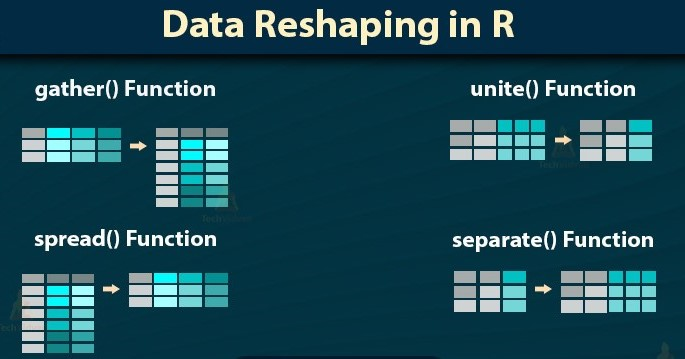
\includegraphics{images/reshape.jpg}

}

\end{figure}

R programlama dilinde \textbf{\texttt{tidyr}} paketinin içinde bulunan
\textbf{\texttt{gather()}}, \textbf{\texttt{spread()}},
\textbf{\texttt{unite()}}, ve \textbf{\texttt{separate()}} gibi
fonksiyonlar, veri manipülasyonu ve veri dönüşümü işlemlerinde
kullanılır. Bu fonksiyonlar, veri çerçevesi içindeki verileri yeniden
düzenlemek, sütunları birleştirmek veya bölmek, veriyi daha uygun bir
yapıya getirmek için kullanılır.

\textbf{\texttt{gather()}} fonksiyonu, geniş formatlı (wide format)
veriyi uzun formatlı (long format) bir yapıya dönüştürmek için
kullanılır. Genellikle sütun adlarını bir ``anahtar'' sütununda toplamak
için kullanılır.

\begin{Shaded}
\begin{Highlighting}[]
\FunctionTok{library}\NormalTok{(tidyr)}

\NormalTok{veri }\OtherTok{\textless{}{-}} \FunctionTok{data.frame}\NormalTok{(}
  \AttributeTok{isim =} \FunctionTok{c}\NormalTok{(}\StringTok{"Ali"}\NormalTok{, }\StringTok{"Esra"}\NormalTok{),}
  \AttributeTok{Matematik =} \FunctionTok{c}\NormalTok{(}\DecValTok{90}\NormalTok{, }\DecValTok{85}\NormalTok{),}
  \AttributeTok{Fizik =} \FunctionTok{c}\NormalTok{(}\DecValTok{88}\NormalTok{, }\DecValTok{76}\NormalTok{)}
\NormalTok{)}

\NormalTok{uzun\_format\_veri }\OtherTok{\textless{}{-}} \FunctionTok{gather}\NormalTok{(veri, Ders, Not, }\SpecialCharTok{{-}}\NormalTok{isim)}

\FunctionTok{print}\NormalTok{(uzun\_format\_veri)}
\end{Highlighting}
\end{Shaded}

\begin{verbatim}
  isim      Ders Not
1  Ali Matematik  90
2 Esra Matematik  85
3  Ali     Fizik  88
4 Esra     Fizik  76
\end{verbatim}

Bu kod, \textbf{\texttt{Matematik}} ve \textbf{\texttt{Fizik}}
sütunlarını toplar ve bir ``Ders'' sütunu oluşturur.

\textbf{\texttt{spread()}} fonksiyonu, uzun formatlı veriyi geniş
formatlı bir yapıya dönüştürmek için kullanılır. Genellikle ``anahtar''
sütunu içindeki değerleri sütun adları olarak kullanmak için kullanılır.

\begin{Shaded}
\begin{Highlighting}[]
\NormalTok{genis\_format\_veri }\OtherTok{\textless{}{-}} \FunctionTok{spread}\NormalTok{(uzun\_format\_veri, Ders, Not)}

\FunctionTok{print}\NormalTok{(genis\_format\_veri)}
\end{Highlighting}
\end{Shaded}

\begin{verbatim}
  isim Fizik Matematik
1  Ali    88        90
2 Esra    76        85
\end{verbatim}

Bu kod, ``Ders'' sütunundaki değerleri sütun adlarına dönüştürür.

\textbf{\texttt{unite()}} fonksiyonu, iki veya daha fazla sütunu
birleştirerek yeni bir sütun oluşturmak için kullanılır.

\begin{Shaded}
\begin{Highlighting}[]
\NormalTok{veri }\OtherTok{\textless{}{-}} \FunctionTok{data.frame}\NormalTok{(}
  \AttributeTok{Ad =} \FunctionTok{c}\NormalTok{(}\StringTok{"Ali"}\NormalTok{, }\StringTok{"Esra"}\NormalTok{),}
  \AttributeTok{Soyad =} \FunctionTok{c}\NormalTok{(}\StringTok{"Yılmaz"}\NormalTok{, }\StringTok{"Mutlu"}\NormalTok{)}
\NormalTok{)}

\NormalTok{veri }\OtherTok{\textless{}{-}} \FunctionTok{unite}\NormalTok{(veri, AdSoyad, Ad, Soyad, }\AttributeTok{sep =} \StringTok{" "}\NormalTok{)}

\FunctionTok{print}\NormalTok{(veri)}
\end{Highlighting}
\end{Shaded}

\begin{verbatim}
     AdSoyad
1 Ali Yılmaz
2 Esra Mutlu
\end{verbatim}

Bu kod, ``Ad'' ve ``Soyad'' sütunlarını birleştirerek ``AdSoyad''
sütununu oluşturur.

\textbf{\texttt{separate()}} fonksiyonu, bir sütunu belirli bir ayırıcı
karakterle bölmek için kullanılır. Bölen değerleri yeni sütunlarda
saklar.

\begin{Shaded}
\begin{Highlighting}[]
\NormalTok{veri }\OtherTok{\textless{}{-}} \FunctionTok{data.frame}\NormalTok{(}
  \AttributeTok{AdSoyad =} \FunctionTok{c}\NormalTok{(}\StringTok{"Ali Yılmaz"}\NormalTok{, }\StringTok{"Esra Mutlu"}\NormalTok{)}
\NormalTok{)}

\NormalTok{veri }\OtherTok{\textless{}{-}} \FunctionTok{separate}\NormalTok{(veri, AdSoyad, }\FunctionTok{c}\NormalTok{(}\StringTok{"Ad"}\NormalTok{, }\StringTok{"Soyad"}\NormalTok{), }\AttributeTok{sep =} \StringTok{" "}\NormalTok{)}

\FunctionTok{print}\NormalTok{(veri)}
\end{Highlighting}
\end{Shaded}

\begin{verbatim}
    Ad  Soyad
1  Ali Yılmaz
2 Esra  Mutlu
\end{verbatim}

Bu kod, ``AdSoyad'' sütununu boşluk karakterine göre böler ve ``Ad'' ve
``Soyad'' sütunlarını oluşturur.

\begin{tcolorbox}[enhanced jigsaw, colbacktitle=quarto-callout-tip-color!10!white, toprule=.15mm, breakable, titlerule=0mm, arc=.35mm, coltitle=black, colframe=quarto-callout-tip-color-frame, opacityback=0, bottomtitle=1mm, colback=white, toptitle=1mm, bottomrule=.15mm, rightrule=.15mm, left=2mm, title=\textcolor{quarto-callout-tip-color}{\faLightbulb}\hspace{0.5em}{Tavsiye}, leftrule=.75mm, opacitybacktitle=0.6]

Bu fonksiyonlar, veri çerçevesi içindeki verileri dönüştürmek ve
düzenlemek için oldukça kullanışlıdır. Veri analizi sürecinde veri
çerçevesini istediğiniz formata getirmek ve veriyi daha iyi anlamak için
bu fonksiyonları kullanabilirsiniz. Daha ileri seviyede kullanmak için
fonksiyonların argümanlarının nasıl kullanıldığını help kısmından ya da
internetten araştırmanızı tavsiye ederim.

Ayrıca \textbf{\texttt{gather}} ve \textbf{\texttt{spread}}
fonksiyonları yerine bunların daha kullanışlı bir karşılığı olan
\textbf{\texttt{pivot\_longer}} ve \textbf{\texttt{pivot\_wider}}
fonksiyonlarını da tercih edebilirsiniz. Bu konudaki örnekleri
incelemenizi tavisye ederim. Belki bunları daha çok sevebilirsiniz.

\end{tcolorbox}

\hypertarget{join}{%
\section*{join}\label{join}}
\addcontentsline{toc}{section}{join}

\markright{join}

\begin{figure}

{\centering 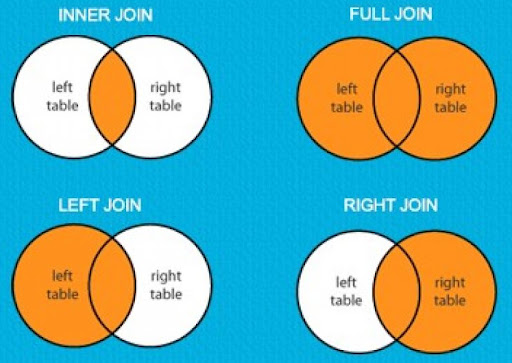
\includegraphics{images/join.jpg}

}

\end{figure}

R programlama dilinde \textbf{\texttt{dplyr}} paketinde bulunan
\textbf{\texttt{left\_join()}}, \textbf{\texttt{right\_join()}},
\textbf{\texttt{inner\_join()}}, ve \textbf{\texttt{full\_join()}} gibi
fonksiyonlar, veri çerçeveleri veya veri tabloları arasında birleştirme
(join) işlemleri yapmak için kullanılır. Bu fonksiyonlar, farklı veri
kaynaklarını birleştirmenizi veya ilişkilendirmenizi sağlar.

\textbf{\texttt{left\_join()}} fonksiyonu, sol veri çerçevesi ile sağ
veri çerçevesi arasında birleştirme işlemi yapar ve sol veri
çerçevesindeki tüm gözlemleri korur. Eğer sağ veri çerçevesinde eşleşen
gözlem yoksa, NA değerleri ile doldurulur.

\begin{Shaded}
\begin{Highlighting}[]
\NormalTok{veri1 }\OtherTok{\textless{}{-}} \FunctionTok{data.frame}\NormalTok{(}
\NormalTok{  Oğrenci }\OtherTok{=} \FunctionTok{c}\NormalTok{(}\StringTok{"Ali"}\NormalTok{, }\StringTok{"Esra"}\NormalTok{, }\StringTok{"Osman"}\NormalTok{),}
  \AttributeTok{Puan1 =} \FunctionTok{c}\NormalTok{(}\DecValTok{90}\NormalTok{, }\DecValTok{85}\NormalTok{, }\DecValTok{78}\NormalTok{)}
\NormalTok{)}

\NormalTok{veri2 }\OtherTok{\textless{}{-}} \FunctionTok{data.frame}\NormalTok{(}
\NormalTok{  Oğrenci }\OtherTok{=} \FunctionTok{c}\NormalTok{(}\StringTok{"Ali"}\NormalTok{, }\StringTok{"Derya"}\NormalTok{, }\StringTok{"Merve"}\NormalTok{),}
  \AttributeTok{Puan2 =} \FunctionTok{c}\NormalTok{(}\DecValTok{88}\NormalTok{, }\DecValTok{92}\NormalTok{, }\DecValTok{85}\NormalTok{)}
\NormalTok{)}

\NormalTok{birlesik\_veri }\OtherTok{\textless{}{-}} \FunctionTok{left\_join}\NormalTok{(veri1, veri2, }\AttributeTok{by =} \StringTok{"Oğrenci"}\NormalTok{)}

\FunctionTok{print}\NormalTok{(birlesik\_veri)}
\end{Highlighting}
\end{Shaded}

\begin{verbatim}
  Oğrenci Puan1 Puan2
1     Ali    90    88
2    Esra    85    NA
3   Osman    78    NA
\end{verbatim}

Bu kod, ``Öğrenci'' sütununa göre iki veri çerçevesini birleştirir. Sol
veri çerçevesi (\textbf{\texttt{veri1}}) tüm gözlemleri içerir ve sağ
veri çerçevesinde (\textbf{\texttt{veri2}}) eşleşen değerler varsa
birleştirir.

\textbf{\texttt{right\_join()}} fonksiyonu,
\textbf{\texttt{left\_join()}} ile benzerdir, ancak sağ veri
çerçevesindeki tüm gözlemleri korur. Eğer sol veri çerçevesinde eşleşen
gözlem yoksa, NA değerleri ile doldurulur.

\begin{Shaded}
\begin{Highlighting}[]
\NormalTok{birlesik\_veri }\OtherTok{\textless{}{-}} \FunctionTok{right\_join}\NormalTok{(veri1, veri2, }\AttributeTok{by =} \StringTok{"Oğrenci"}\NormalTok{)}

\FunctionTok{print}\NormalTok{(birlesik\_veri)}
\end{Highlighting}
\end{Shaded}

\begin{verbatim}
  Oğrenci Puan1 Puan2
1     Ali    90    88
2   Derya    NA    92
3   Merve    NA    85
\end{verbatim}

Bu kod, sağ veri çerçevesi (\textbf{\texttt{veri2}}) tüm gözlemleri
içerir ve sol veri çerçevesinde (\textbf{\texttt{veri1}}) eşleşen
değerler varsa birleştirir.

\textbf{\texttt{inner\_join()}} fonksiyonu, sol ve sağ veri çerçeveleri
arasında iç birleştirme yapar ve yalnızca ortak gözlemleri korur. Ortak
gözlemleri içermeyen diğer gözlemleri atar.

\begin{Shaded}
\begin{Highlighting}[]
\NormalTok{birlesik\_veri }\OtherTok{\textless{}{-}} \FunctionTok{inner\_join}\NormalTok{(veri1, veri2, }\AttributeTok{by =} \StringTok{"Oğrenci"}\NormalTok{)}

\FunctionTok{print}\NormalTok{(birlesik\_veri)}
\end{Highlighting}
\end{Shaded}

\begin{verbatim}
  Oğrenci Puan1 Puan2
1     Ali    90    88
\end{verbatim}

Bu kod, sadece sol ve sağ veri çerçevelerinde (\textbf{\texttt{veri1}}
ve \textbf{\texttt{veri2}}) ortak olan gözlemleri korur.

\textbf{\texttt{full\_join()}} fonksiyonu, sol ve sağ veri çerçeveleri
arasında tam birleştirme yapar ve tüm gözlemleri korur. Ortak olmayan
değerler NA ile doldurulur.

\begin{Shaded}
\begin{Highlighting}[]
\NormalTok{birlesik\_veri }\OtherTok{\textless{}{-}} \FunctionTok{full\_join}\NormalTok{(veri1, veri2, }\AttributeTok{by =} \StringTok{"Oğrenci"}\NormalTok{)}

\FunctionTok{print}\NormalTok{(birlesik\_veri)}
\end{Highlighting}
\end{Shaded}

\begin{verbatim}
  Oğrenci Puan1 Puan2
1     Ali    90    88
2    Esra    85    NA
3   Osman    78    NA
4   Derya    NA    92
5   Merve    NA    85
\end{verbatim}

Bu kod, sol ve sağ veri çerçevelerini (\textbf{\texttt{veri1}} ve
\textbf{\texttt{veri2}}) tamamen birleştirir ve tüm gözlemleri içerir.

\begin{tcolorbox}[enhanced jigsaw, colbacktitle=quarto-callout-note-color!10!white, toprule=.15mm, breakable, titlerule=0mm, arc=.35mm, coltitle=black, colframe=quarto-callout-note-color-frame, opacityback=0, bottomtitle=1mm, colback=white, toptitle=1mm, bottomrule=.15mm, rightrule=.15mm, left=2mm, title=\textcolor{quarto-callout-note-color}{\faInfo}\hspace{0.5em}{Not}, leftrule=.75mm, opacitybacktitle=0.6]

Bu dört join fonksiyonu, farklı veri kaynaklarını birleştirme
işlemlerinde kullanılır ve veri analizi sürecinde verileri daha kapsamlı
bir şekilde incelemek için oldukça kullanışlıdır. Hangi join işleminin
kullanılacağı, veri yapısına ve ihtiyaca bağlı olarak değişebilir.

\end{tcolorbox}

\bookmarksetup{startatroot}

\hypertarget{keux15fifuxe7i-veri-analizi}{%
\chapter*{Keşifçi Veri Analizi}\label{keux15fifuxe7i-veri-analizi}}
\addcontentsline{toc}{chapter}{Keşifçi Veri Analizi}

\markboth{Keşifçi Veri Analizi}{Keşifçi Veri Analizi}

Keşifçi Veri Analizi (Exploratory Data Analysis veya kısaca EDA), veri
setinizi anlamak, içindeki örüntüleri ve ilişkileri belirlemek ve olası
sorunları tanımlamak amacıyla veriye yakından bakmanızı sağlayan bir
veri analizi yaklaşımıdır. EDA, verileri tanımanıza veya verilerdeki
olası özellikler ve ilişkiler hakkında daha derin bir anlayış
kazanmanıza yardımcı olabilir. EDA, yeni bir şey değildir, ancak EDA,
birkaç nedenden dolayı yakın geçmişte önemli ölçüde büyümüştür:

\begin{itemize}
\item
  Veriler her zamankinden daha hızlı ve daha büyük miktarlarda
  üretiliyor, bu yüzden incelememiz gereken çok şey var.
\item
  Bilgisayarlar ve yazılımlar (R gibi) EDA yapma fırsatlarını
  genişletmiştir.
\item
  İstatistiksel model seçeneklerindeki artış, genellikle doğrudan
  geleneksel bir modele gitmek yerine verilerimize daha yakından
  bakmamızı gerektirmektedir.
\end{itemize}

EDA, verilerinizin nihai analizi açısından genellikle istatistiksel
değildir, ancak EDA'nın geçiş süreci olarak düşünülmesi gerekir. EDA'dan
öğrendikleriniz modellemenize rehberlik edecek ve istatistiksel araçlar
hakkında verdiğiniz kararları doğrudan bilgilendirecektir. R gibi
programlama dilleri ve istatistiksel araçlar, EDA sürecini
kolaylaştırmak ve verileri görselleştirmek için kullanışlıdır. EDA, veri
madenciliği ve veri bilimi projelerinin başlangıcında sıklıkla
kullanılır ve aşağıdaki adımları içerir:

\begin{enumerate}
\def\labelenumi{\arabic{enumi}.}
\item
  \textbf{Veri İçe Aktarma:} İlk adım, analiz yapmak için veriyi içe
  aktarmaktır. Veriyi R ortamına çeşitli formatlardan (CSV, Excel, SQL
  veritabanları, vb.) içe aktarabilirsiniz.
\item
  \textbf{Veriye Genel Bakış:} Veri setinize ilk bakışta, kaç gözlem ve
  değişken olduğunu, değişken türlerini (sayısal, kategorik, metinsel
  vb.) ve eksik verilerin varlığını incelemelisiniz. Bu bilgi, veri
  hakkında ilk fikirlerinizi oluşturmanıza yardımcı olur.
\item
  \textbf{Veri Görselleştirme:} Verileri görselleştirmek, EDA'nın önemli
  bir parçasıdır. R'nin ggplot2 gibi kütüphaneleri, verilerinizi
  grafiklerle görselleştirmek için kullanışlı araçlar sunar.
  Histogramlar, kutu grafikleri, çubuk grafikleri ve dağılım grafikleri
  gibi grafikler oluşturarak verilerinizi daha iyi anlayabilirsiniz.
\item
  \textbf{Merkezi Eğilim ve Dağılım Ölçüleri:} Veri setinizin merkezi
  eğilimini (ortalama, medyan, mod) ve dağılımını (standart sapma,
  varyans, çeyrekler arası aralık) hesaplayarak verilerinizin genel
  özelliklerini değerlendirebilirsiniz.
\item
  \textbf{Değişkenler Arası İlişkiler:} Değişkenler arasındaki
  ilişkileri anlamak için korelasyon analizi, scatter plotlar ve faktör
  analizi gibi teknikleri kullanabilirsiniz.
\item
  \textbf{Aykırı Değerler ve Eksik Veriler:} Aykırı değerleri tanımlayın
  ve bunların analiz üzerindeki etkilerini değerlendirin. Ayrıca eksik
  verileri ele alın (örneğin, eksik verileri doldurma veya eksik
  gözlemleri çıkarma).
\item
  \textbf{Veri Gruplama ve Alt Kümelere Bölme:} İhtiyaca göre veriyi
  gruplara ayırabilir veya alt kümeler oluşturabilirsiniz. Bu, farklı
  veri alt kümeleri arasındaki farkları incelemek için kullanışlı
  olabilir.
\item
  \textbf{Hipotez Testleri ve İstatistiksel Analiz:} EDA süreci
  sırasında, veriler üzerinde belirli hipotezleri test etmek için
  istatistiksel testler (t-test, ANOVA, vb.) uygulayabilirsiniz. Bu,
  verilerinizde anlamlı farklılıkları veya özellikleri tespit etmenize
  yardımcı olur.
\item
  \textbf{Sonuçların Yorumlanması:} EDA sürecinin sonunda, elde edilen
  sonuçları yorumlamalı ve bulgularınızı raporlamalısınız. Bulgularınız,
  daha sonraki analiz aşamaları veya veri madenciliği projeleri için
  temel oluşturur.
\end{enumerate}

EDA, veri analizi sürecinin önemli bir parçasıdır çünkü veriyi daha iyi
anlamanızı ve daha ileri analizler için yol haritasını belirlemenizi
sağlar. Aynı zamanda veri setinizdeki hataları veya tutarsızlıkları
tespit etmenize ve düzeltmenize de yardımcı olur.

\hypertarget{veri-ile-tanux131ux15fma}{%
\section*{Veri ile Tanışma}\label{veri-ile-tanux131ux15fma}}
\addcontentsline{toc}{section}{Veri ile Tanışma}

\markright{Veri ile Tanışma}

Veri analizinin başlangıç aşamasında, verinin yapısına, ne tür
değişkenler içerdiğine, çeşitli özet istatistiklerine bakmak ve gerekli
ise ne tür dönüşümler yapmak gerektiğini bilmek önemlidir. Bu süreçler
daha derin analizlere daha kolay devam edebilmek için de önemlidir.
Bunları gerçekleştirmek için hem özet tablolar hem de grafikler
yardımıyla verileri tanımak gerekmektedir.

Tek ve iki değişkenli olarak sayısal ve kategorik veri analizi
\href{https://ggplot2.tidyverse.org/reference/mpg.html}{\ul{\textbf{mpg}}}
verisi kullanılarak yapılacaktır. Bu veri setinde 38 farklı aracın yakıt
verileri bulunmaktadır.

\begin{Shaded}
\begin{Highlighting}[]
\CommentTok{\# mpg verisi ggplot2 paketinde olduğundan paketi çağırıyoruz}
\FunctionTok{library}\NormalTok{(ggplot2)}

\FunctionTok{head}\NormalTok{(mpg)}
\end{Highlighting}
\end{Shaded}

\begin{verbatim}
# A tibble: 6 x 11
  manufacturer model displ  year   cyl trans      drv     cty   hwy fl    class 
  <chr>        <chr> <dbl> <int> <int> <chr>      <chr> <int> <int> <chr> <chr> 
1 audi         a4      1.8  1999     4 auto(l5)   f        18    29 p     compa~
2 audi         a4      1.8  1999     4 manual(m5) f        21    29 p     compa~
3 audi         a4      2    2008     4 manual(m6) f        20    31 p     compa~
4 audi         a4      2    2008     4 auto(av)   f        21    30 p     compa~
5 audi         a4      2.8  1999     6 auto(l5)   f        16    26 p     compa~
6 audi         a4      2.8  1999     6 manual(m5) f        18    26 p     compa~
\end{verbatim}

\begin{Shaded}
\begin{Highlighting}[]
\FunctionTok{nrow}\NormalTok{(mpg)}
\end{Highlighting}
\end{Shaded}

\begin{verbatim}
[1] 234
\end{verbatim}

\begin{Shaded}
\begin{Highlighting}[]
\FunctionTok{ncol}\NormalTok{(mpg)}
\end{Highlighting}
\end{Shaded}

\begin{verbatim}
[1] 11
\end{verbatim}

\begin{Shaded}
\begin{Highlighting}[]
\FunctionTok{str}\NormalTok{(mpg)}
\end{Highlighting}
\end{Shaded}

\begin{verbatim}
tibble [234 x 11] (S3: tbl_df/tbl/data.frame)
 $ manufacturer: chr [1:234] "audi" "audi" "audi" "audi" ...
 $ model       : chr [1:234] "a4" "a4" "a4" "a4" ...
 $ displ       : num [1:234] 1.8 1.8 2 2 2.8 2.8 3.1 1.8 1.8 2 ...
 $ year        : int [1:234] 1999 1999 2008 2008 1999 1999 2008 1999 1999 2008 ...
 $ cyl         : int [1:234] 4 4 4 4 6 6 6 4 4 4 ...
 $ trans       : chr [1:234] "auto(l5)" "manual(m5)" "manual(m6)" "auto(av)" ...
 $ drv         : chr [1:234] "f" "f" "f" "f" ...
 $ cty         : int [1:234] 18 21 20 21 16 18 18 18 16 20 ...
 $ hwy         : int [1:234] 29 29 31 30 26 26 27 26 25 28 ...
 $ fl          : chr [1:234] "p" "p" "p" "p" ...
 $ class       : chr [1:234] "compact" "compact" "compact" "compact" ...
\end{verbatim}

\begin{Shaded}
\begin{Highlighting}[]
\FunctionTok{colnames}\NormalTok{(mpg)}
\end{Highlighting}
\end{Shaded}

\begin{verbatim}
 [1] "manufacturer" "model"        "displ"        "year"         "cyl"         
 [6] "trans"        "drv"          "cty"          "hwy"          "fl"          
[11] "class"       
\end{verbatim}

\begin{Shaded}
\begin{Highlighting}[]
\FunctionTok{summary}\NormalTok{(mpg)}
\end{Highlighting}
\end{Shaded}

\begin{verbatim}
 manufacturer          model               displ            year     
 Length:234         Length:234         Min.   :1.600   Min.   :1999  
 Class :character   Class :character   1st Qu.:2.400   1st Qu.:1999  
 Mode  :character   Mode  :character   Median :3.300   Median :2004  
                                       Mean   :3.472   Mean   :2004  
                                       3rd Qu.:4.600   3rd Qu.:2008  
                                       Max.   :7.000   Max.   :2008  
      cyl           trans               drv                 cty       
 Min.   :4.000   Length:234         Length:234         Min.   : 9.00  
 1st Qu.:4.000   Class :character   Class :character   1st Qu.:14.00  
 Median :6.000   Mode  :character   Mode  :character   Median :17.00  
 Mean   :5.889                                         Mean   :16.86  
 3rd Qu.:8.000                                         3rd Qu.:19.00  
 Max.   :8.000                                         Max.   :35.00  
      hwy             fl               class          
 Min.   :12.00   Length:234         Length:234        
 1st Qu.:18.00   Class :character   Class :character  
 Median :24.00   Mode  :character   Mode  :character  
 Mean   :23.44                                        
 3rd Qu.:27.00                                        
 Max.   :44.00                                        
\end{verbatim}

\begin{Shaded}
\begin{Highlighting}[]
\NormalTok{df }\OtherTok{\textless{}{-}}\NormalTok{ mpg}

\CommentTok{\# class değişkenini faktöre çevirip, kategorilerine bakalım}
\NormalTok{df}\SpecialCharTok{$}\NormalTok{class }\OtherTok{\textless{}{-}} \FunctionTok{factor}\NormalTok{(df}\SpecialCharTok{$}\NormalTok{class)}
\FunctionTok{levels}\NormalTok{(df}\SpecialCharTok{$}\NormalTok{class)}
\end{Highlighting}
\end{Shaded}

\begin{verbatim}
[1] "2seater"    "compact"    "midsize"    "minivan"    "pickup"    
[6] "subcompact" "suv"       
\end{verbatim}

\begin{Shaded}
\begin{Highlighting}[]
\NormalTok{dplyr}\SpecialCharTok{::}\FunctionTok{glimpse}\NormalTok{(df)}
\end{Highlighting}
\end{Shaded}

\begin{verbatim}
Rows: 234
Columns: 11
$ manufacturer <chr> "audi", "audi", "audi", "audi", "audi", "audi", "audi", "~
$ model        <chr> "a4", "a4", "a4", "a4", "a4", "a4", "a4", "a4 quattro", "~
$ displ        <dbl> 1.8, 1.8, 2.0, 2.0, 2.8, 2.8, 3.1, 1.8, 1.8, 2.0, 2.0, 2.~
$ year         <int> 1999, 1999, 2008, 2008, 1999, 1999, 2008, 1999, 1999, 200~
$ cyl          <int> 4, 4, 4, 4, 6, 6, 6, 4, 4, 4, 4, 6, 6, 6, 6, 6, 6, 8, 8, ~
$ trans        <chr> "auto(l5)", "manual(m5)", "manual(m6)", "auto(av)", "auto~
$ drv          <chr> "f", "f", "f", "f", "f", "f", "f", "4", "4", "4", "4", "4~
$ cty          <int> 18, 21, 20, 21, 16, 18, 18, 18, 16, 20, 19, 15, 17, 17, 1~
$ hwy          <int> 29, 29, 31, 30, 26, 26, 27, 26, 25, 28, 27, 25, 25, 25, 2~
$ fl           <chr> "p", "p", "p", "p", "p", "p", "p", "p", "p", "p", "p", "p~
$ class        <fct> compact, compact, compact, compact, compact, compact, com~
\end{verbatim}

\hypertarget{suxfcrekli-deux11fiux15fkenler}{%
\section*{Sürekli Değişkenler}\label{suxfcrekli-deux11fiux15fkenler}}
\addcontentsline{toc}{section}{Sürekli Değişkenler}

\markright{Sürekli Değişkenler}

Veri analizi, birçok farklı değişken türünün incelenmesini gerektirir.
Bu değişkenler arasında sürekli değişkenler özellikle önemlidir. Sürekli
değişkenler, belirli bir aralıktaki değerleri alabilen ve sonsuz sayıda
mümkün değer içeren değişkenlerdir. Örnek olarak, yaş, gelir, sıcaklık
gibi değerler sürekli değişkenlere örnektir. Sürekli değişkenlerin
analizi, verileri anlamak ve içindeki örüntüleri keşfetmek için
kullanılır. Bu analiz, genellikle aşağıdaki adımları içerir:

\begin{enumerate}
\def\labelenumi{\arabic{enumi}.}
\item
  \textbf{Veri Görselleştirme:}Sürekli değişkenlerin analizine başlamak
  için verilerinizi görselleştirmek önemlidir. Histogramlar, kutu
  grafikleri, yoğunluk grafikleri ve saçılım grafikleri gibi grafikler,
  veri dağılımını ve örüntülerini görsel olarak incelemenize yardımcı
  olur. Bu grafikler, veri setinizin merkezi eğilimini (ortalama veya
  medyan), yayılımını ve aykırı değerleri hızla görmeye yardımcı olur.
\item
  \textbf{Merkezi Eğilim ve Dağılım Ölçüleri:} Sürekli değişkenlerin
  merkezi eğilimini ve dağılımını hesaplamak verileri özetlemenin önemli
  bir yoludur. Bu ölçümler, veri setinin merkezi noktasını ve veri
  noktalarının nasıl dağıldığını anlamamıza yardımcı olur. Örnek olarak,
  ortalama (mean), medyan (median), standart sapma (standard deviation)
  ve varyans (variance) gibi ölçümler bu aşamada kullanılır.
\item
  \textbf{Korelasyon Analizi:} Eğer birden fazla sürekli değişken
  arasındaki ilişkiyi anlamak istiyorsanız, korelasyon analizi
  yapabilirsiniz. Korelasyon, iki değişken arasındaki ilişkinin gücünü
  ve yönünü ölçer. Korelasyon katsayısı, bu ilişkiyi değerlendirmek için
  kullanılır. Pozitif bir korelasyon, iki değişkenin aynı yönde
  değiştiğini, negatif bir korelasyon ise iki değişkenin ters yönde
  değiştiğini gösterir.
\item
  \textbf{Hipotez Testleri:} Sürekli değişkenler arasındaki
  farklılıkları değerlendirmek için hipotez testleri kullanılabilir.
  Örneğin, iki grup arasındaki ortalama değerlerin istatistiksel olarak
  anlamlı bir farklılık gösterip göstermediğini belirlemek için
  t-testleri veya ANOVA analizi kullanılabilir.
\item
  \textbf{Güven Aralıkları:} Sürekli değişkenlerin analizi sırasında,
  belirli bir parametre (örneğin, ortalama) hakkında güven aralıkları
  hesaplanabilir. Bu güven aralıkları, parametrenin belirli bir güven
  düzeyinde bulunduğu aralığı gösterir. Bu, parametrenin tahmini
  kesinliğini değerlendirmek için kullanışlıdır.
\end{enumerate}

Sürekli değişkenlerin analizi, verileri anlama ve kararlarınızı
destekleme sürecinin önemli bir parçasıdır. İyi bir analiz, veri
setinizdeki örüntüleri ve ilişkileri açığa çıkarmanıza yardımcı olur ve
bilinçli kararlar almanıza yardımcı olur. Bu nedenle, sürekli
değişkenlerin analizi yaparken yukarıda belirtilen adımları takip etmek
önemlidir.

\begin{Shaded}
\begin{Highlighting}[]
\CommentTok{\# cty ve hwy değişkenlerini inceleyelim. }
\CommentTok{\# cty şehiriçi, hwy şehirarasını ifade ediyor.}

\FunctionTok{summary}\NormalTok{(df}\SpecialCharTok{$}\NormalTok{cty)}
\end{Highlighting}
\end{Shaded}

\begin{verbatim}
   Min. 1st Qu.  Median    Mean 3rd Qu.    Max. 
   9.00   14.00   17.00   16.86   19.00   35.00 
\end{verbatim}

\begin{Shaded}
\begin{Highlighting}[]
\FunctionTok{var}\NormalTok{(df}\SpecialCharTok{$}\NormalTok{cty)}
\end{Highlighting}
\end{Shaded}

\begin{verbatim}
[1] 18.11307
\end{verbatim}

\begin{Shaded}
\begin{Highlighting}[]
\FunctionTok{mean}\NormalTok{(df}\SpecialCharTok{$}\NormalTok{cty)}
\end{Highlighting}
\end{Shaded}

\begin{verbatim}
[1] 16.85897
\end{verbatim}

\begin{Shaded}
\begin{Highlighting}[]
\FunctionTok{summary}\NormalTok{(df}\SpecialCharTok{$}\NormalTok{hwy)}
\end{Highlighting}
\end{Shaded}

\begin{verbatim}
   Min. 1st Qu.  Median    Mean 3rd Qu.    Max. 
  12.00   18.00   24.00   23.44   27.00   44.00 
\end{verbatim}

\begin{Shaded}
\begin{Highlighting}[]
\FunctionTok{var}\NormalTok{(df}\SpecialCharTok{$}\NormalTok{hwy)}
\end{Highlighting}
\end{Shaded}

\begin{verbatim}
[1] 35.45778
\end{verbatim}

\begin{Shaded}
\begin{Highlighting}[]
\FunctionTok{mean}\NormalTok{(df}\SpecialCharTok{$}\NormalTok{hwy)}
\end{Highlighting}
\end{Shaded}

\begin{verbatim}
[1] 23.44017
\end{verbatim}

\begin{Shaded}
\begin{Highlighting}[]
\CommentTok{\# 1 mile= 1.609 km}
\CommentTok{\# 1 galon = 3.79 lt}

\CommentTok{\# litre başına km hesaplama}
\NormalTok{galonmil\_to\_ltkm }\OtherTok{\textless{}{-}} \ControlFlowTok{function}\NormalTok{(x)\{}
  
\NormalTok{  km }\OtherTok{\textless{}{-}}\NormalTok{ x }\SpecialCharTok{*} \FloatTok{1.609}\SpecialCharTok{/}\FloatTok{3.79}
  \FunctionTok{return}\NormalTok{(km)}
\NormalTok{\}}

\NormalTok{df}\SpecialCharTok{$}\NormalTok{cty\_ltkm }\OtherTok{\textless{}{-}} \FunctionTok{galonmil\_to\_ltkm}\NormalTok{(df}\SpecialCharTok{$}\NormalTok{cty)}
\NormalTok{df}\SpecialCharTok{$}\NormalTok{hwy\_ltkm }\OtherTok{\textless{}{-}} \FunctionTok{galonmil\_to\_ltkm}\NormalTok{(df}\SpecialCharTok{$}\NormalTok{hwy)}
\FunctionTok{quantile}\NormalTok{(df}\SpecialCharTok{$}\NormalTok{cty\_ltkm) }
\end{Highlighting}
\end{Shaded}

\begin{verbatim}
       0%       25%       50%       75%      100% 
 3.820844  5.943536  7.217150  8.066227 14.858839 
\end{verbatim}

\begin{Shaded}
\begin{Highlighting}[]
\CommentTok{\# şehiriçi araçların \% 75\textquotesingle{}i 1 lt ile 8.06 km den az yol alıyor.}
\FunctionTok{quantile}\NormalTok{(df}\SpecialCharTok{$}\NormalTok{hwy\_ltkm)}
\end{Highlighting}
\end{Shaded}

\begin{verbatim}
       0%       25%       50%       75%      100% 
 5.094459  7.641689 10.188918 11.462533 18.679683 
\end{verbatim}

\begin{Shaded}
\begin{Highlighting}[]
\CommentTok{\# şehirlerarası araçların \% 75\textquotesingle{}i 1 lt ile 11.46 km den az yol alıyor.}


\CommentTok{\# değişken dağılımı için histogram grafiği kullanılabilir.}
\FunctionTok{hist}\NormalTok{(df}\SpecialCharTok{$}\NormalTok{cty\_ltkm,}\AttributeTok{freq =} \ConstantTok{FALSE}\NormalTok{,}\AttributeTok{col =} \StringTok{"red"}\NormalTok{,}\AttributeTok{border =} \StringTok{"blue"}\NormalTok{)}
\FunctionTok{lines}\NormalTok{(}\FunctionTok{density}\NormalTok{(df}\SpecialCharTok{$}\NormalTok{cty\_ltkm), }\AttributeTok{col =} \StringTok{"black"}\NormalTok{, }\AttributeTok{lwd =} \DecValTok{2}\NormalTok{,)}
\end{Highlighting}
\end{Shaded}

\begin{figure}[H]

{\centering 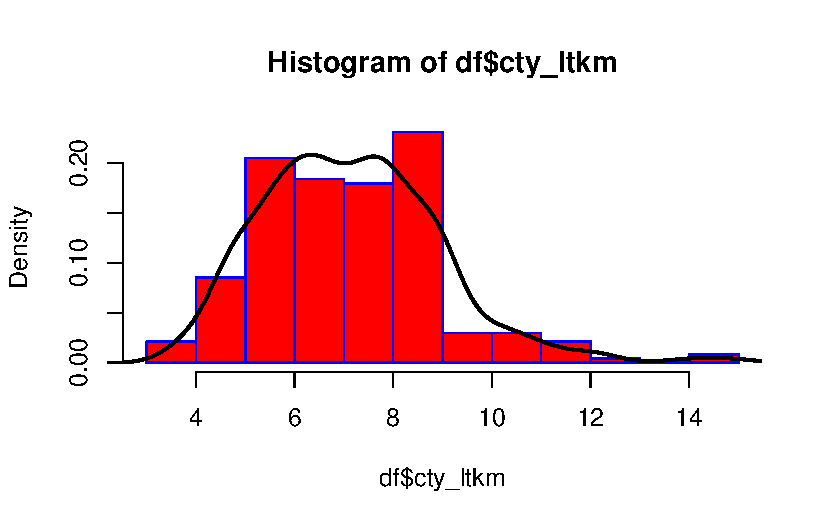
\includegraphics{data_analysis_files/figure-pdf/unnamed-chunk-2-1.pdf}

}

\end{figure}

\begin{Shaded}
\begin{Highlighting}[]
\FunctionTok{hist}\NormalTok{(df}\SpecialCharTok{$}\NormalTok{hwy\_ltkm,}\AttributeTok{xlim =} \FunctionTok{c}\NormalTok{(}\DecValTok{4}\NormalTok{,}\DecValTok{20}\NormalTok{), }\AttributeTok{ylim =} \FunctionTok{c}\NormalTok{(}\DecValTok{0}\NormalTok{,}\DecValTok{60}\NormalTok{), }\AttributeTok{breaks =} \DecValTok{10}\NormalTok{)}
\end{Highlighting}
\end{Shaded}

\begin{figure}[H]

{\centering \includegraphics{data_analysis_files/figure-pdf/unnamed-chunk-2-2.pdf}

}

\end{figure}

\begin{Shaded}
\begin{Highlighting}[]
\CommentTok{\# Boxplot}
\FunctionTok{boxplot}\NormalTok{(df}\SpecialCharTok{$}\NormalTok{cty\_ltkm, }\AttributeTok{main =} \StringTok{"Boxplot cty"}\NormalTok{)}
\end{Highlighting}
\end{Shaded}

\begin{figure}[H]

{\centering \includegraphics{data_analysis_files/figure-pdf/unnamed-chunk-2-3.pdf}

}

\end{figure}

\begin{Shaded}
\begin{Highlighting}[]
\FunctionTok{fivenum}\NormalTok{(df}\SpecialCharTok{$}\NormalTok{cty\_ltkm) }\CommentTok{\# minimum, Q1, median, Q3, maximum}
\end{Highlighting}
\end{Shaded}

\begin{verbatim}
[1]  3.820844  5.943536  7.217150  8.066227 14.858839
\end{verbatim}

\begin{Shaded}
\begin{Highlighting}[]
\CommentTok{\# outliers }
\FunctionTok{boxplot}\NormalTok{(df}\SpecialCharTok{$}\NormalTok{cty\_ltkm)}\SpecialCharTok{$}\NormalTok{out}
\end{Highlighting}
\end{Shaded}

\begin{figure}[H]

{\centering 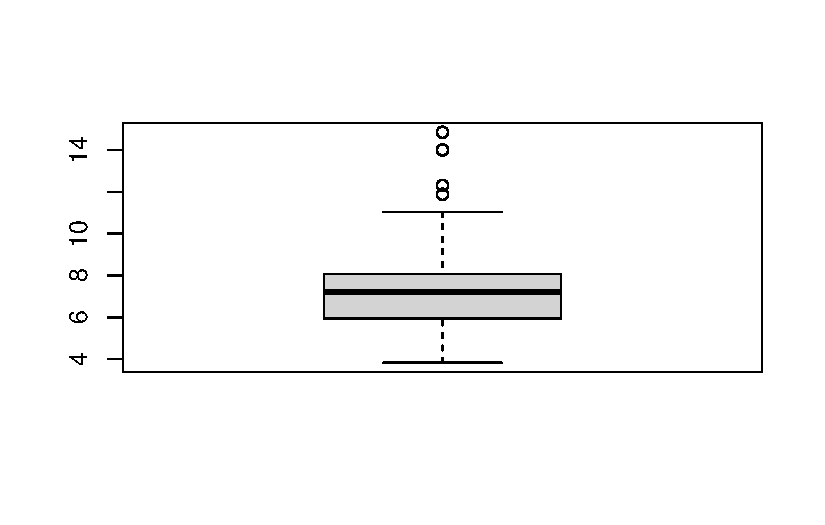
\includegraphics{data_analysis_files/figure-pdf/unnamed-chunk-2-4.pdf}

}

\end{figure}

\begin{verbatim}
[1] 11.88707 11.88707 14.00976 14.85884 12.31161
\end{verbatim}

\begin{Shaded}
\begin{Highlighting}[]
\CommentTok{\# outliers hangi sıralarda}
\FunctionTok{which}\NormalTok{(df}\SpecialCharTok{$}\NormalTok{cty\_ltkm }\SpecialCharTok{\%in\%} \FunctionTok{boxplot}\NormalTok{(df}\SpecialCharTok{$}\NormalTok{cty\_ltkm)}\SpecialCharTok{$}\NormalTok{out)}
\end{Highlighting}
\end{Shaded}

\begin{verbatim}
[1] 100 197 213 222 223
\end{verbatim}

\begin{Shaded}
\begin{Highlighting}[]
\FunctionTok{boxplot}\NormalTok{(df}\SpecialCharTok{$}\NormalTok{hwy\_ltkm, }\AttributeTok{main =} \StringTok{"Boxplot cty"}\NormalTok{)}
\end{Highlighting}
\end{Shaded}

\begin{figure}[H]

{\centering 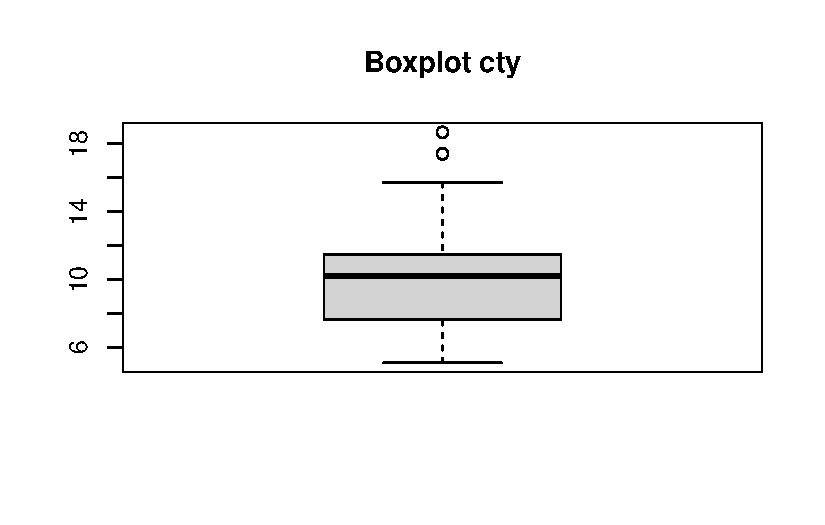
\includegraphics{data_analysis_files/figure-pdf/unnamed-chunk-2-5.pdf}

}

\end{figure}

\begin{Shaded}
\begin{Highlighting}[]
\FunctionTok{fivenum}\NormalTok{(df}\SpecialCharTok{$}\NormalTok{hwy\_ltkm) }\CommentTok{\# minimum, Q1, median, Q3, maximum}
\end{Highlighting}
\end{Shaded}

\begin{verbatim}
[1]  5.094459  7.641689 10.188918 11.462533 18.679683
\end{verbatim}

\begin{Shaded}
\begin{Highlighting}[]
\FunctionTok{boxplot}\NormalTok{(hwy\_ltkm }\SpecialCharTok{\textasciitilde{}}\NormalTok{ cyl, }\AttributeTok{data =}\NormalTok{ df, }\AttributeTok{xlab =} \StringTok{"Silindir Sayısı"}\NormalTok{,}
   \AttributeTok{ylab =} \StringTok{"Litre Başına KM"}\NormalTok{, }\AttributeTok{main =} \StringTok{"Mileage Data"}\NormalTok{)}
\end{Highlighting}
\end{Shaded}

\begin{figure}[H]

{\centering 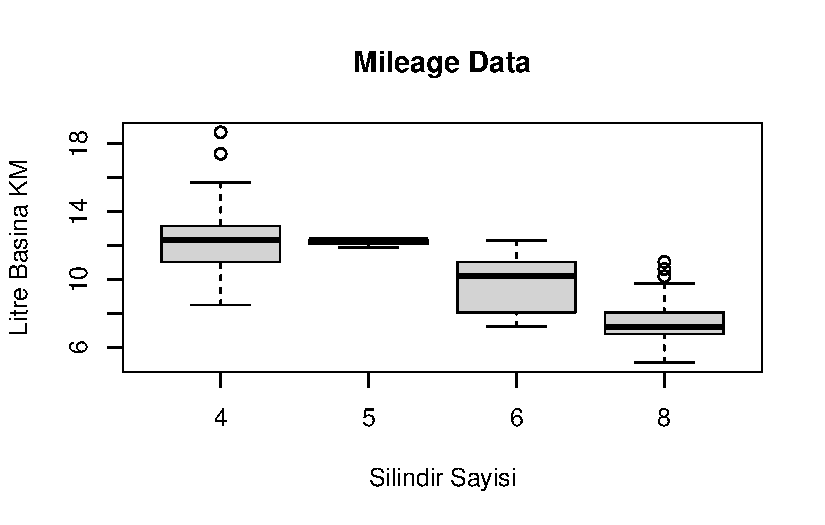
\includegraphics{data_analysis_files/figure-pdf/unnamed-chunk-2-6.pdf}

}

\end{figure}

\begin{Shaded}
\begin{Highlighting}[]
\FunctionTok{boxplot}\NormalTok{(hwy\_ltkm }\SpecialCharTok{\textasciitilde{}}\NormalTok{ cyl, }\AttributeTok{data =}\NormalTok{ df, }
   \AttributeTok{xlab =} \StringTok{"Silindir Sayısı"}\NormalTok{,}
   \AttributeTok{ylab =} \StringTok{"Litre Başına KM"}\NormalTok{, }
   \AttributeTok{main =} \StringTok{"Mileage Data"}\NormalTok{,}
   \AttributeTok{notch =} \ConstantTok{TRUE}\NormalTok{, }
   \AttributeTok{varwidth =} \ConstantTok{TRUE}\NormalTok{, }
   \AttributeTok{col =} \FunctionTok{c}\NormalTok{(}\StringTok{"green"}\NormalTok{,}\StringTok{"yellow"}\NormalTok{,}\StringTok{"purple"}\NormalTok{,}\StringTok{"blue"}\NormalTok{),}
   \AttributeTok{names =} \FunctionTok{c}\NormalTok{(}\StringTok{"2 Silindir"}\NormalTok{,}\StringTok{"4 Silindir"}\NormalTok{,}\StringTok{"6 Silindir"}\NormalTok{,}\StringTok{"8 Silindir"}\NormalTok{)}
\NormalTok{)}
\end{Highlighting}
\end{Shaded}

\begin{verbatim}
Warning in (function (z, notch = FALSE, width = NULL, varwidth = FALSE, : some
notches went outside hinges ('box'): maybe set notch=FALSE
\end{verbatim}

\begin{figure}[H]

{\centering 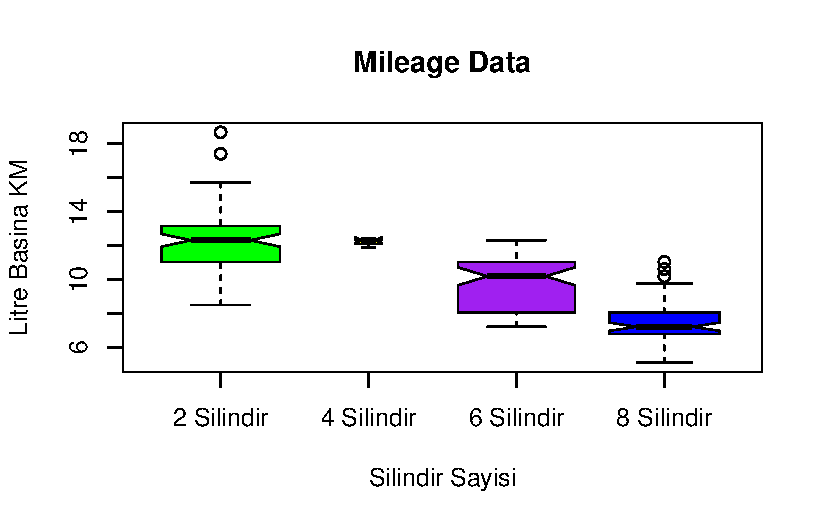
\includegraphics{data_analysis_files/figure-pdf/unnamed-chunk-2-7.pdf}

}

\end{figure}

\begin{Shaded}
\begin{Highlighting}[]
\CommentTok{\# Sürekli iki değişken incelemek istersek;}

\CommentTok{\# displ ve cty\_ltkm değişkenlerini inceleyelim}
\CommentTok{\# displ motor hacmini ifade ediyor}

\FunctionTok{summary}\NormalTok{(df}\SpecialCharTok{$}\NormalTok{displ)}
\end{Highlighting}
\end{Shaded}

\begin{verbatim}
   Min. 1st Qu.  Median    Mean 3rd Qu.    Max. 
  1.600   2.400   3.300   3.472   4.600   7.000 
\end{verbatim}

\begin{Shaded}
\begin{Highlighting}[]
\FunctionTok{with}\NormalTok{(df,}\FunctionTok{cor}\NormalTok{(displ,cty\_ltkm))}
\end{Highlighting}
\end{Shaded}

\begin{verbatim}
[1] -0.798524
\end{verbatim}

\begin{Shaded}
\begin{Highlighting}[]
\CommentTok{\# motor hacmi ile lt başına km ters ilişkili}

\FunctionTok{plot}\NormalTok{(df}\SpecialCharTok{$}\NormalTok{displ,df}\SpecialCharTok{$}\NormalTok{cty\_ltkm, }
     \AttributeTok{main =} \StringTok{"Motor Hacmi{-} Yakıt Tüketimi Saçılım Grafiği"}\NormalTok{,}
     \AttributeTok{col=}\StringTok{"red"}\NormalTok{,}
     \AttributeTok{xlab =} \StringTok{"Motor Hacmi"}\NormalTok{,}
     \AttributeTok{ylab =} \StringTok{"Yakıt Tüketimi"}\NormalTok{)}
\end{Highlighting}
\end{Shaded}

\begin{figure}[H]

{\centering 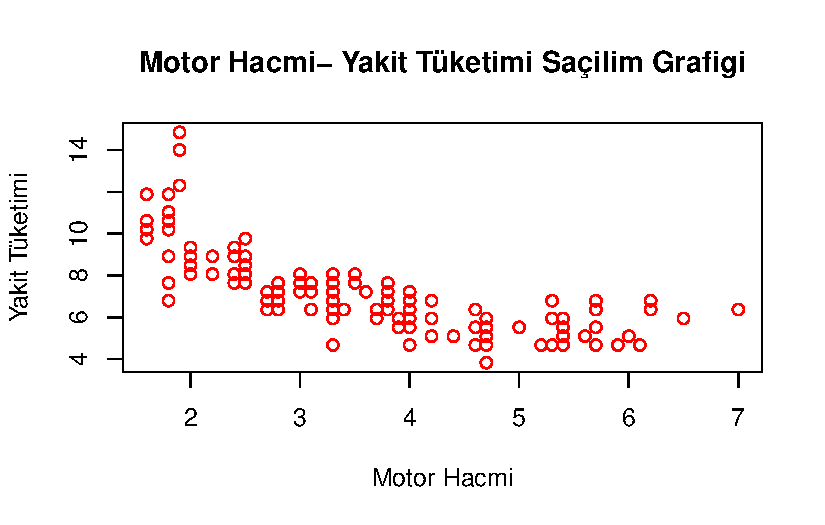
\includegraphics{data_analysis_files/figure-pdf/unnamed-chunk-2-8.pdf}

}

\end{figure}

\begin{Shaded}
\begin{Highlighting}[]
\CommentTok{\# birden fazla değişkenin saçılım grafiği}
\FunctionTok{pairs}\NormalTok{(}\SpecialCharTok{\textasciitilde{}}\NormalTok{hwy\_ltkm}\SpecialCharTok{+}\NormalTok{cty\_ltkm}\SpecialCharTok{+}\NormalTok{displ}\SpecialCharTok{+}\NormalTok{cyl,}\AttributeTok{data =}\NormalTok{ df,}\AttributeTok{main =} \StringTok{"Scatterplot Matrix"}\NormalTok{)}
\end{Highlighting}
\end{Shaded}

\begin{figure}[H]

{\centering 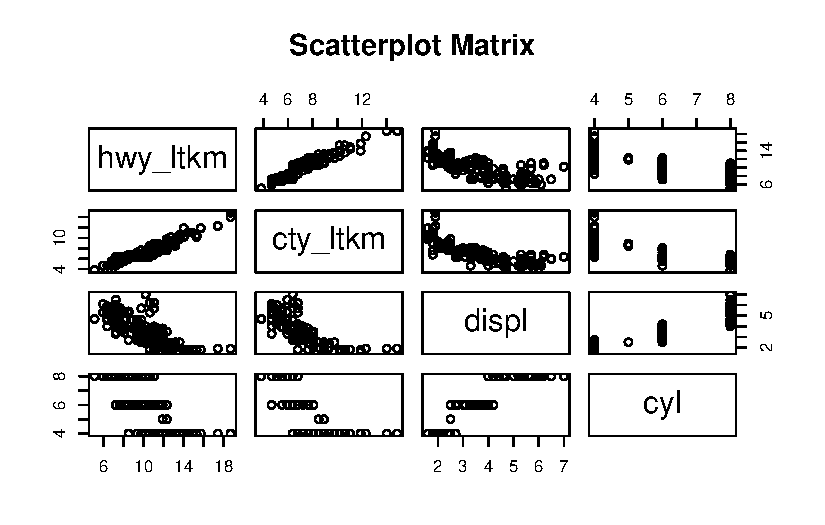
\includegraphics{data_analysis_files/figure-pdf/unnamed-chunk-2-9.pdf}

}

\end{figure}

\hypertarget{kategorik-deux11fiux15fkenler}{%
\section*{Kategorik Değişkenler}\label{kategorik-deux11fiux15fkenler}}
\addcontentsline{toc}{section}{Kategorik Değişkenler}

\markright{Kategorik Değişkenler}

Veri analizi sürecinde, kategorik değişkenler (veya gruplar) genellikle
çok önemli bir rol oynar. Kategorik değişkenler, belirli bir sınıfı veya
kategoriyi temsil eden değişkenlerdir ve tipik olarak metin veya
sembollerle ifade edilirler. Örnek olarak, cinsiyet, eğitim seviyesi,
ürün kategorileri gibi değişkenler kategorik değişkenlere örnektir.
Kategorik değişkenlerin analizi, bu değişkenlerin içindeki örüntüleri,
dağılımları ve ilişkileri anlamamıza yardımcı olur. Aşağıda, kategorik
değişkenlerin analizi için izlenebilecek temel adımları bulabilirsiniz:

\begin{enumerate}
\def\labelenumi{\arabic{enumi}.}
\item
  \textbf{Frekans Tabloları ve Görselleştirme:} Kategorik değişkenlerin
  frekans tablolarını ve grafiklerini oluşturarak, her kategori veya
  sınıfın veri setinde ne kadar sık görüldüğünü anlayabilirsiniz.
  Örneğin, bar grafikleri, pasta grafikleri veya çubuk grafikleri
  kullanarak kategori frekanslarını görselleştirebilirsiniz.
  \textbf{\texttt{summary()}} ve \textbf{\texttt{table()}} gibi R
  fonksiyonları ile bu verileri inceleyebilirsiniz.
\item
  \textbf{İlişkileri İnceleme:} Kategorik değişkenler arasındaki
  ilişkileri anlamak önemlidir. İki kategorik değişken arasındaki
  ilişkiyi değerlendirmek için çapraz tablolar (cross-tabulation) ve
  ki-kare (chi-squared) istatistiksel testleri kullanabilirsiniz. Bu
  testler, iki değişken arasındaki bağımlılığı değerlendirmek için
  kullanılır.
\item
  \textbf{İstatistiksel Testler:} Kategorik değişkenlerin analizi
  sırasında, gruplar arasındaki farkları değerlendirmek için hipotez
  testleri kullanabilirsiniz. İki kategorik değişken arasındaki
  ilişkinin istatistiksel olarak anlamlı olup olmadığını belirlemek için
  ki-kare testi veya Fisher'in kesin testi gibi testler
  kullanabilirsiniz. Ayrıca ANOVA gibi testler, bir kategorik değişkenin
  birden fazla grup üzerindeki etkisini değerlendirmek için
  kullanılabilir.
\item
  \textbf{Veri Görselleştirme:} Kategorik değişkenlerin analizinde,
  gruplar arasındaki farkları daha iyi anlamak için grafikler
  kullanabilirsiniz. Bar grafikleri, grupların frekanslarını
  görselleştirmek için sıklıkla kullanılırken, gruplar arasındaki
  ilişkiyi anlamak için mozaik grafikleri veya heatmap'leri de
  kullanabilirsiniz.
\end{enumerate}

Kategorik değişkenlerin analizi, veri setinizin içindeki desenleri ve
ilişkileri anlamanıza yardımcı olur. Bu analiz, kararlarınızı
desteklemek ve veriyi daha iyi anlamak için önemlidir. R programlama
dili, kategorik değişkenlerin analizi için bir dizi kullanışlı fonksiyon
ve paket sunar. Bu adımları takip ederek, veri analiz projelerinizde
kategorik değişkenleri etkili bir şekilde analiz edebilirsiniz.

\begin{Shaded}
\begin{Highlighting}[]
\CommentTok{\# class ve trans değişkenlerine bakalım}
\CommentTok{\# class araç sınıfı, trans ise vites türünü ifade ediyor.}

\FunctionTok{summary}\NormalTok{(df}\SpecialCharTok{$}\NormalTok{class)}
\end{Highlighting}
\end{Shaded}

\begin{verbatim}
   2seater    compact    midsize    minivan     pickup subcompact        suv 
         5         47         41         11         33         35         62 
\end{verbatim}

\begin{Shaded}
\begin{Highlighting}[]
\FunctionTok{table}\NormalTok{(df}\SpecialCharTok{$}\NormalTok{class)}
\end{Highlighting}
\end{Shaded}

\begin{verbatim}

   2seater    compact    midsize    minivan     pickup subcompact        suv 
         5         47         41         11         33         35         62 
\end{verbatim}

\begin{Shaded}
\begin{Highlighting}[]
\FunctionTok{xtabs}\NormalTok{(}\SpecialCharTok{\textasciitilde{}}\NormalTok{class,}\AttributeTok{data=}\NormalTok{df)}
\end{Highlighting}
\end{Shaded}

\begin{verbatim}
class
   2seater    compact    midsize    minivan     pickup subcompact        suv 
         5         47         41         11         33         35         62 
\end{verbatim}

\begin{Shaded}
\begin{Highlighting}[]
\FunctionTok{table}\NormalTok{(df}\SpecialCharTok{$}\NormalTok{trans)}
\end{Highlighting}
\end{Shaded}

\begin{verbatim}

  auto(av)   auto(l3)   auto(l4)   auto(l5)   auto(l6)   auto(s4)   auto(s5) 
         5          2         83         39          6          3          3 
  auto(s6) manual(m5) manual(m6) 
        16         58         19 
\end{verbatim}

\begin{Shaded}
\begin{Highlighting}[]
\FunctionTok{prop.table}\NormalTok{(}\FunctionTok{table}\NormalTok{(df}\SpecialCharTok{$}\NormalTok{class))}
\end{Highlighting}
\end{Shaded}

\begin{verbatim}

   2seater    compact    midsize    minivan     pickup subcompact        suv 
0.02136752 0.20085470 0.17521368 0.04700855 0.14102564 0.14957265 0.26495726 
\end{verbatim}

\begin{Shaded}
\begin{Highlighting}[]
\NormalTok{tab }\OtherTok{\textless{}{-}} \FunctionTok{table}\NormalTok{(df}\SpecialCharTok{$}\NormalTok{class)}
\FunctionTok{barplot}\NormalTok{(tab,}\AttributeTok{col=}\StringTok{"blue"}\NormalTok{,}\AttributeTok{border=}\StringTok{"red"}\NormalTok{)}
\end{Highlighting}
\end{Shaded}

\begin{figure}[H]

{\centering 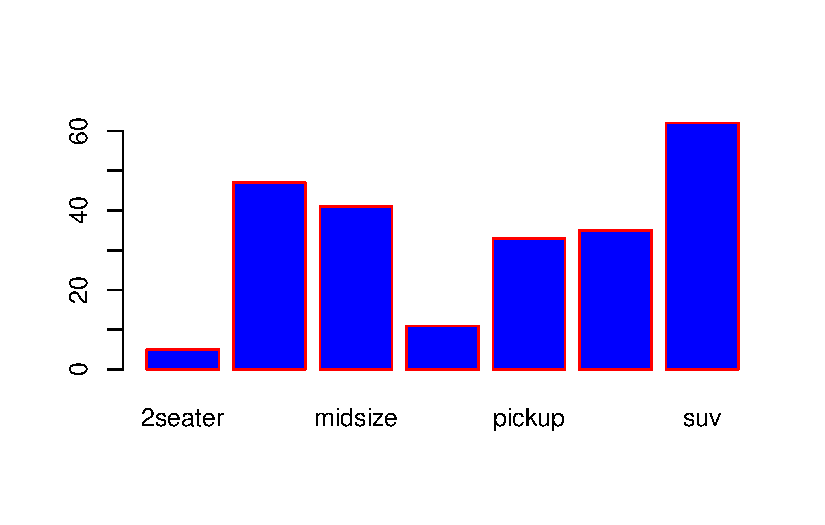
\includegraphics{data_analysis_files/figure-pdf/unnamed-chunk-3-1.pdf}

}

\end{figure}

\begin{Shaded}
\begin{Highlighting}[]
\FunctionTok{pie}\NormalTok{(tab)}
\end{Highlighting}
\end{Shaded}

\begin{figure}[H]

{\centering 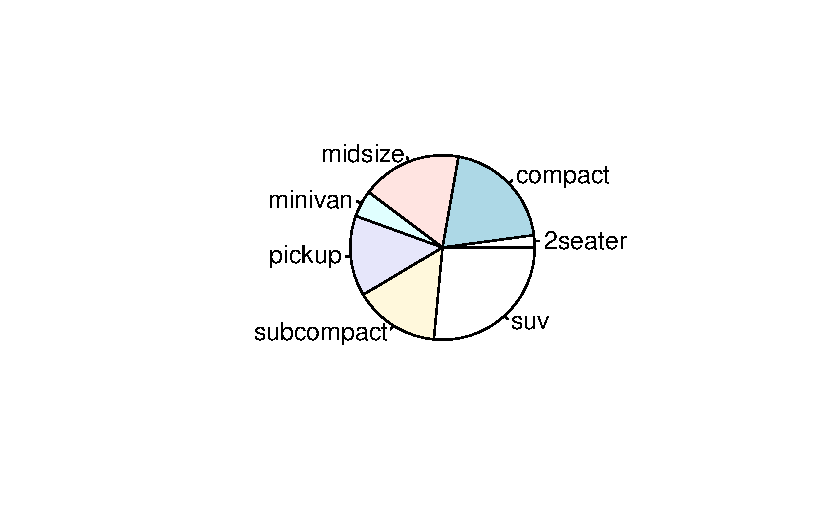
\includegraphics{data_analysis_files/figure-pdf/unnamed-chunk-3-2.pdf}

}

\end{figure}

\begin{Shaded}
\begin{Highlighting}[]
\FunctionTok{par}\NormalTok{(}\AttributeTok{mfrow =} \FunctionTok{c}\NormalTok{(}\DecValTok{1}\NormalTok{, }\DecValTok{2}\NormalTok{))}
\FunctionTok{barplot}\NormalTok{(tab)}
\FunctionTok{pie}\NormalTok{(tab)}
\end{Highlighting}
\end{Shaded}

\begin{figure}[H]

{\centering 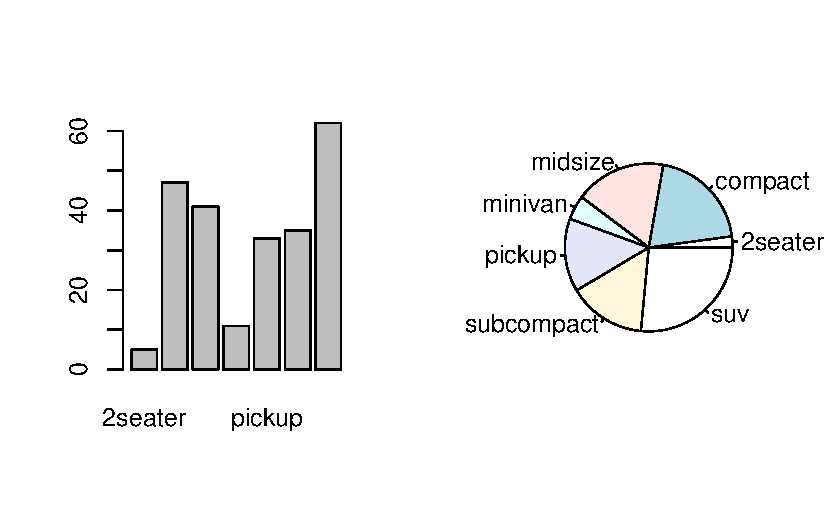
\includegraphics{data_analysis_files/figure-pdf/unnamed-chunk-3-3.pdf}

}

\end{figure}

\begin{Shaded}
\begin{Highlighting}[]
\CommentTok{\# Kategorik iki değişken incelemek istersek;}

\FunctionTok{xtabs}\NormalTok{(}\SpecialCharTok{\textasciitilde{}}\NormalTok{trans}\SpecialCharTok{+}\NormalTok{class,}\AttributeTok{data=}\NormalTok{df)}
\end{Highlighting}
\end{Shaded}

\begin{verbatim}
            class
trans        2seater compact midsize minivan pickup subcompact suv
  auto(av)         0       2       3       0      0          0   0
  auto(l3)         0       1       0       1      0          0   0
  auto(l4)         1       8      14       8     12         11  29
  auto(l5)         0       4       5       0      8          4  18
  auto(l6)         0       0       0       2      0          0   4
  auto(s4)         0       2       1       0      0          0   0
  auto(s5)         0       2       0       0      0          0   1
  auto(s6)         1       5       6       0      0          1   3
  manual(m5)       0      18       9       0      8         16   7
  manual(m6)       3       5       3       0      5          3   0
\end{verbatim}

\begin{Shaded}
\begin{Highlighting}[]
\FunctionTok{prop.table}\NormalTok{(}\FunctionTok{table}\NormalTok{(df}\SpecialCharTok{$}\NormalTok{year,df}\SpecialCharTok{$}\NormalTok{class),}\DecValTok{1}\NormalTok{) }\CommentTok{\# satır toplamları 1\textquotesingle{} eşittir}
\end{Highlighting}
\end{Shaded}

\begin{verbatim}
      
          2seater    compact    midsize    minivan     pickup subcompact
  1999 0.01709402 0.21367521 0.17094017 0.05128205 0.13675214 0.16239316
  2008 0.02564103 0.18803419 0.17948718 0.04273504 0.14529915 0.13675214
      
              suv
  1999 0.24786325
  2008 0.28205128
\end{verbatim}

\begin{Shaded}
\begin{Highlighting}[]
\FunctionTok{prop.table}\NormalTok{(}\FunctionTok{table}\NormalTok{(df}\SpecialCharTok{$}\NormalTok{year,df}\SpecialCharTok{$}\NormalTok{class),}\DecValTok{2}\NormalTok{) }\CommentTok{\# sütun toplamları 1\textquotesingle{} eşittir}
\end{Highlighting}
\end{Shaded}

\begin{verbatim}
      
         2seater   compact   midsize   minivan    pickup subcompact       suv
  1999 0.4000000 0.5319149 0.4878049 0.5454545 0.4848485  0.5428571 0.4677419
  2008 0.6000000 0.4680851 0.5121951 0.4545455 0.5151515  0.4571429 0.5322581
\end{verbatim}

\begin{Shaded}
\begin{Highlighting}[]
\FunctionTok{proportions}\NormalTok{(}\FunctionTok{xtabs}\NormalTok{(}\SpecialCharTok{\textasciitilde{}}\NormalTok{ manufacturer }\SpecialCharTok{+}\NormalTok{ year, }\AttributeTok{data =}\NormalTok{ df), }\DecValTok{1}\NormalTok{)}
\end{Highlighting}
\end{Shaded}

\begin{verbatim}
            year
manufacturer      1999      2008
  audi       0.5000000 0.5000000
  chevrolet  0.3684211 0.6315789
  dodge      0.4324324 0.5675676
  ford       0.6000000 0.4000000
  honda      0.5555556 0.4444444
  hyundai    0.4285714 0.5714286
  jeep       0.2500000 0.7500000
  land rover 0.5000000 0.5000000
  lincoln    0.6666667 0.3333333
  mercury    0.5000000 0.5000000
  nissan     0.4615385 0.5384615
  pontiac    0.6000000 0.4000000
  subaru     0.4285714 0.5714286
  toyota     0.5882353 0.4117647
  volkswagen 0.5925926 0.4074074
\end{verbatim}

\begin{Shaded}
\begin{Highlighting}[]
\CommentTok{\# araç sınıfı ile drv değişkenine birlikte bakalım}
\CommentTok{\# f = front{-}wheel drive (önden çekiş), }
\CommentTok{\# r = rear wheel drive (arkadan çekiş), }
\CommentTok{\# 4 = 4wd (4 çeker)}

\FunctionTok{plot}\NormalTok{(class }\SpecialCharTok{\textasciitilde{}} \FunctionTok{factor}\NormalTok{(drv), }\AttributeTok{data =}\NormalTok{ df)}
\end{Highlighting}
\end{Shaded}

\begin{figure}[H]

{\centering 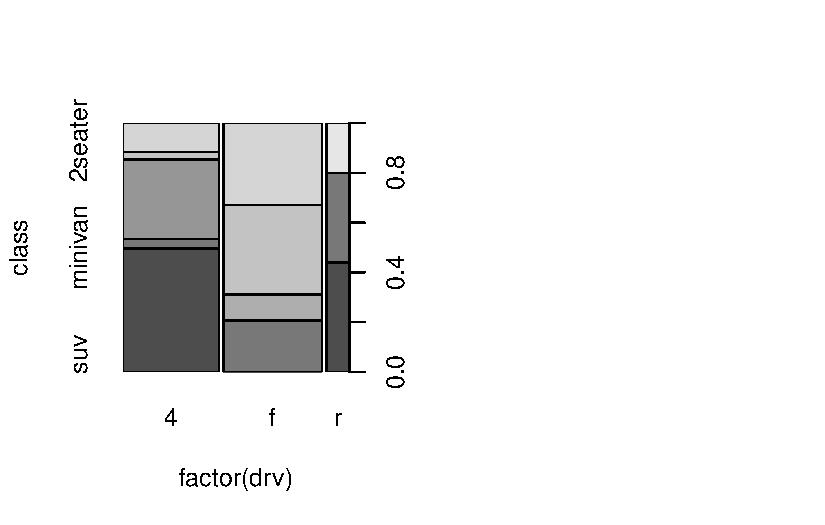
\includegraphics{data_analysis_files/figure-pdf/unnamed-chunk-3-4.pdf}

}

\end{figure}

Eğer hem sürekli hem de kategorik değişkenleri incelemek istersek,
benzer şekilde görselleştirme ve kategoriler arasında merkezi eğilim
ölçüleri hesaplanabilir. Bunlar dışında uygun istatistiksel testler de
gerçekleştirilebilir.

\begin{Shaded}
\begin{Highlighting}[]
\CommentTok{\# Silindir düzeyinde yakıt tüketimi }
\FunctionTok{tapply}\NormalTok{(df}\SpecialCharTok{$}\NormalTok{cty\_ltkm, df}\SpecialCharTok{$}\NormalTok{cyl, mean)}
\end{Highlighting}
\end{Shaded}

\begin{verbatim}
       4        5        6        8 
8.920545 8.703034 6.883968 5.337052 
\end{verbatim}

\begin{Shaded}
\begin{Highlighting}[]
\CommentTok{\# Same using aggregate()}
\FunctionTok{aggregate}\NormalTok{(cty\_ltkm }\SpecialCharTok{\textasciitilde{}}\NormalTok{ cyl, }\AttributeTok{data =}\NormalTok{ df, }\AttributeTok{FUN =}\NormalTok{ mean)}
\end{Highlighting}
\end{Shaded}

\begin{verbatim}
  cyl cty_ltkm
1   4 8.920545
2   5 8.703034
3   6 6.883968
4   8 5.337052
\end{verbatim}

\begin{Shaded}
\begin{Highlighting}[]
\FunctionTok{boxplot}\NormalTok{(cty\_ltkm }\SpecialCharTok{\textasciitilde{}}\NormalTok{ cyl, }\AttributeTok{data =}\NormalTok{ df)}
\end{Highlighting}
\end{Shaded}

\begin{figure}[H]

{\centering 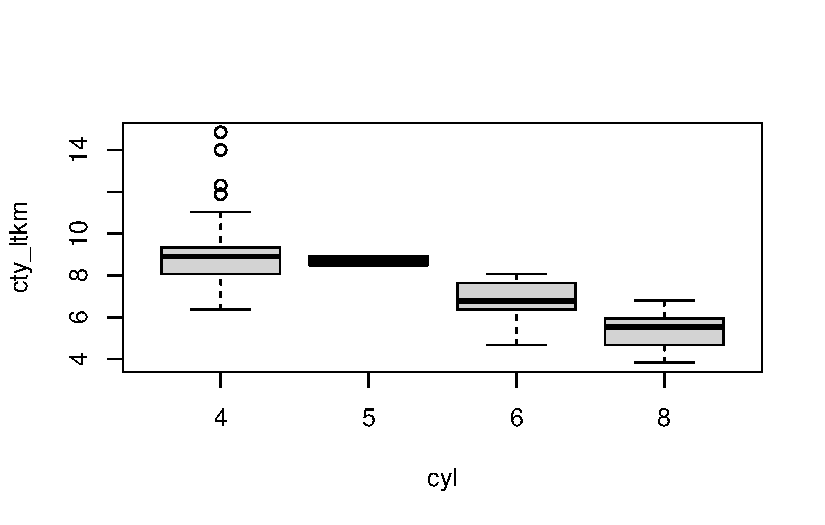
\includegraphics{data_analysis_files/figure-pdf/unnamed-chunk-4-1.pdf}

}

\end{figure}

\hypertarget{zaman-serileri}{%
\section*{Zaman Serileri}\label{zaman-serileri}}
\addcontentsline{toc}{section}{Zaman Serileri}

\markright{Zaman Serileri}

R programlama dili, zaman serileri analizi için kapsamlı bir dizi
fonksiyon ve paket sunar. Zaman serileri analizi, zaman içindeki veri
noktalarının örüntülerini ve trendlerini incelemeyi amaçlar. R'de zaman
serileri ile çalışmak için \textbf{\texttt{ts}} (time series) nesnesi
kullanılır. Bu nesne, zaman serisi verilerini zaman dilimleri (örneğin
aylar, yıllar) veya tarihler ile ilişkilendirerek işlem yapmanıza olanak
tanır.

\begin{Shaded}
\begin{Highlighting}[]
\NormalTok{AirPassengers}
\end{Highlighting}
\end{Shaded}

\begin{verbatim}
     Jan Feb Mar Apr May Jun Jul Aug Sep Oct Nov Dec
1949 112 118 132 129 121 135 148 148 136 119 104 118
1950 115 126 141 135 125 149 170 170 158 133 114 140
1951 145 150 178 163 172 178 199 199 184 162 146 166
1952 171 180 193 181 183 218 230 242 209 191 172 194
1953 196 196 236 235 229 243 264 272 237 211 180 201
1954 204 188 235 227 234 264 302 293 259 229 203 229
1955 242 233 267 269 270 315 364 347 312 274 237 278
1956 284 277 317 313 318 374 413 405 355 306 271 306
1957 315 301 356 348 355 422 465 467 404 347 305 336
1958 340 318 362 348 363 435 491 505 404 359 310 337
1959 360 342 406 396 420 472 548 559 463 407 362 405
1960 417 391 419 461 472 535 622 606 508 461 390 432
\end{verbatim}

\begin{Shaded}
\begin{Highlighting}[]
\FunctionTok{class}\NormalTok{(AirPassengers)}
\end{Highlighting}
\end{Shaded}

\begin{verbatim}
[1] "ts"
\end{verbatim}

\begin{Shaded}
\begin{Highlighting}[]
\FunctionTok{diff}\NormalTok{(AirPassengers) }\CommentTok{\# fark alma}
\end{Highlighting}
\end{Shaded}

\begin{verbatim}
      Jan  Feb  Mar  Apr  May  Jun  Jul  Aug  Sep  Oct  Nov  Dec
1949         6   14   -3   -8   14   13    0  -12  -17  -15   14
1950   -3   11   15   -6  -10   24   21    0  -12  -25  -19   26
1951    5    5   28  -15    9    6   21    0  -15  -22  -16   20
1952    5    9   13  -12    2   35   12   12  -33  -18  -19   22
1953    2    0   40   -1   -6   14   21    8  -35  -26  -31   21
1954    3  -16   47   -8    7   30   38   -9  -34  -30  -26   26
1955   13   -9   34    2    1   45   49  -17  -35  -38  -37   41
1956    6   -7   40   -4    5   56   39   -8  -50  -49  -35   35
1957    9  -14   55   -8    7   67   43    2  -63  -57  -42   31
1958    4  -22   44  -14   15   72   56   14 -101  -45  -49   27
1959   23  -18   64  -10   24   52   76   11  -96  -56  -45   43
1960   12  -26   28   42   11   63   87  -16  -98  -47  -71   42
\end{verbatim}

\begin{Shaded}
\begin{Highlighting}[]
\NormalTok{stats}\SpecialCharTok{::}\FunctionTok{lag}\NormalTok{(AirPassengers,}\SpecialCharTok{{-}}\DecValTok{1}\NormalTok{) }\CommentTok{\# 1. gecikmesini alma}
\end{Highlighting}
\end{Shaded}

\begin{verbatim}
     Jan Feb Mar Apr May Jun Jul Aug Sep Oct Nov Dec
1949     112 118 132 129 121 135 148 148 136 119 104
1950 118 115 126 141 135 125 149 170 170 158 133 114
1951 140 145 150 178 163 172 178 199 199 184 162 146
1952 166 171 180 193 181 183 218 230 242 209 191 172
1953 194 196 196 236 235 229 243 264 272 237 211 180
1954 201 204 188 235 227 234 264 302 293 259 229 203
1955 229 242 233 267 269 270 315 364 347 312 274 237
1956 278 284 277 317 313 318 374 413 405 355 306 271
1957 306 315 301 356 348 355 422 465 467 404 347 305
1958 336 340 318 362 348 363 435 491 505 404 359 310
1959 337 360 342 406 396 420 472 548 559 463 407 362
1960 405 417 391 419 461 472 535 622 606 508 461 390
1961 432                                            
\end{verbatim}

\begin{Shaded}
\begin{Highlighting}[]
\FunctionTok{plot}\NormalTok{(AirPassengers,}\AttributeTok{type =} \StringTok{"p"}\NormalTok{, }\AttributeTok{col =} \StringTok{"red"}\NormalTok{) }\CommentTok{\# points}
\end{Highlighting}
\end{Shaded}

\begin{figure}[H]

{\centering 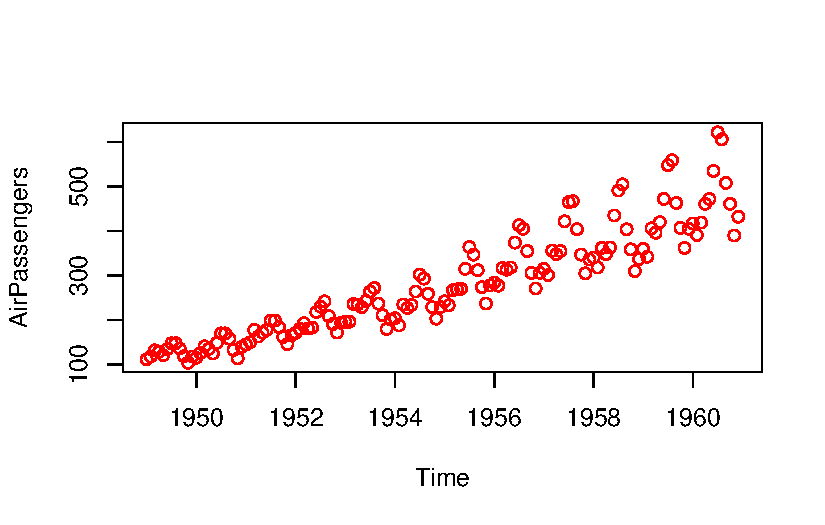
\includegraphics{data_analysis_files/figure-pdf/unnamed-chunk-5-1.pdf}

}

\end{figure}

\begin{Shaded}
\begin{Highlighting}[]
\FunctionTok{plot}\NormalTok{(AirPassengers,}\AttributeTok{type =} \StringTok{"l"}\NormalTok{, }\AttributeTok{col =} \StringTok{"red"}\NormalTok{) }\CommentTok{\# line}
\end{Highlighting}
\end{Shaded}

\begin{figure}[H]

{\centering 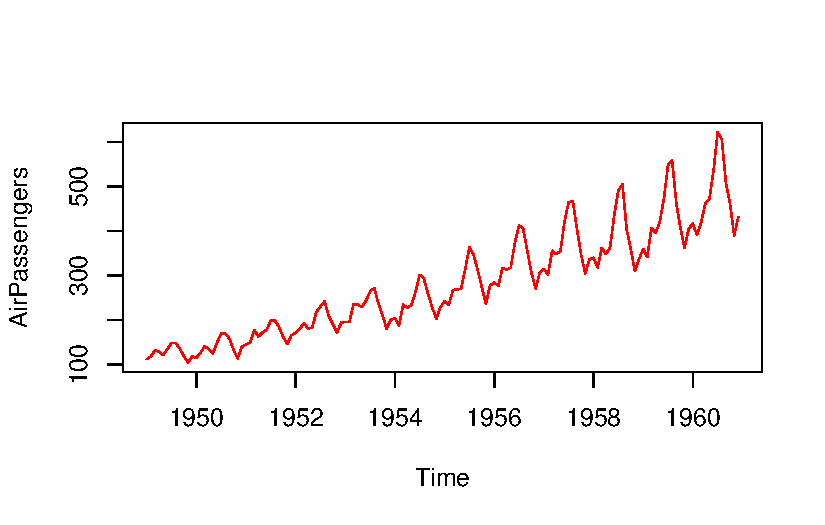
\includegraphics{data_analysis_files/figure-pdf/unnamed-chunk-5-2.pdf}

}

\end{figure}

\begin{Shaded}
\begin{Highlighting}[]
\FunctionTok{plot}\NormalTok{(AirPassengers,}\AttributeTok{type =} \StringTok{"o"}\NormalTok{, }\AttributeTok{col =} \StringTok{"red"}\NormalTok{) }\CommentTok{\# points and line}
\end{Highlighting}
\end{Shaded}

\begin{figure}[H]

{\centering 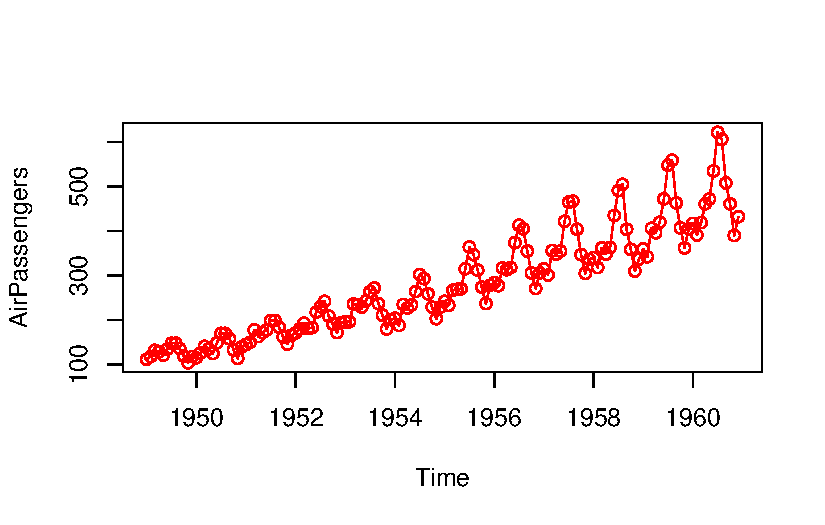
\includegraphics{data_analysis_files/figure-pdf/unnamed-chunk-5-3.pdf}

}

\end{figure}

\begin{Shaded}
\begin{Highlighting}[]
\FunctionTok{plot}\NormalTok{(}\FunctionTok{log}\NormalTok{(AirPassengers),}\AttributeTok{type =} \StringTok{"l"}\NormalTok{, }\AttributeTok{col =} \StringTok{"red"}\NormalTok{) }\CommentTok{\# line}
\end{Highlighting}
\end{Shaded}

\begin{figure}[H]

{\centering 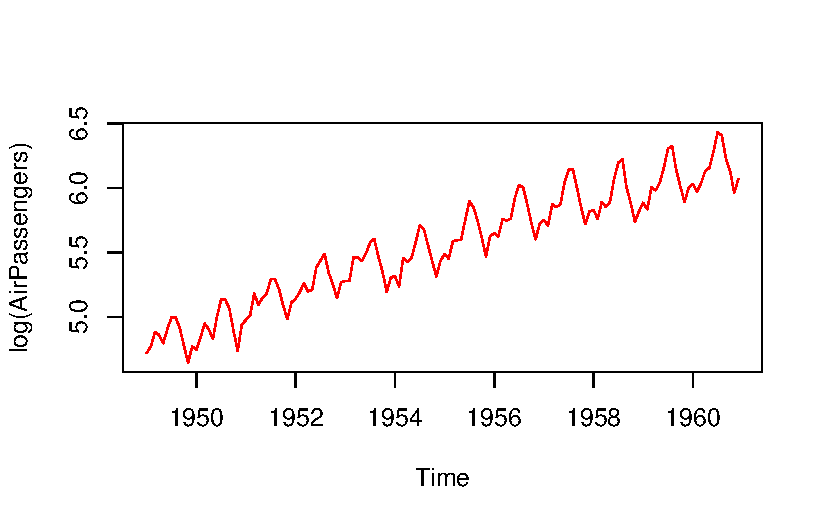
\includegraphics{data_analysis_files/figure-pdf/unnamed-chunk-5-4.pdf}

}

\end{figure}

\begin{Shaded}
\begin{Highlighting}[]
\FunctionTok{plot}\NormalTok{(}\FunctionTok{diff}\NormalTok{(AirPassengers),}\AttributeTok{type =} \StringTok{"l"}\NormalTok{, }\AttributeTok{col =} \StringTok{"red"}\NormalTok{) }\CommentTok{\# line}
\end{Highlighting}
\end{Shaded}

\begin{figure}[H]

{\centering 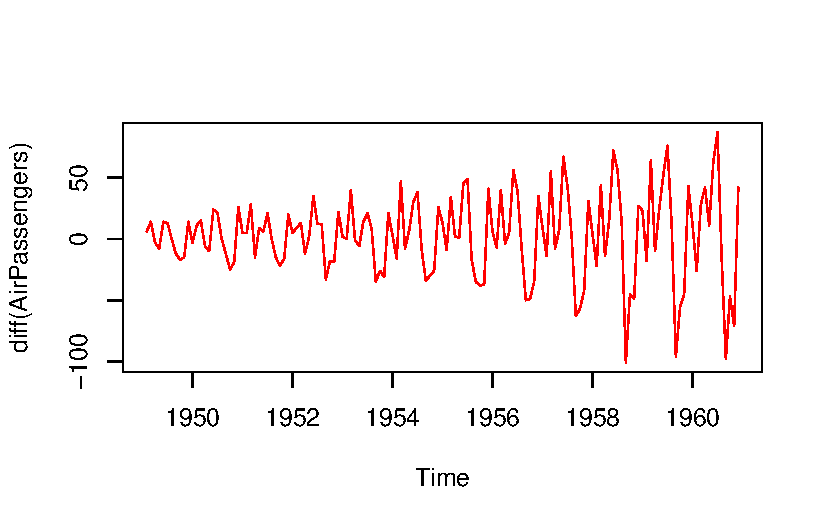
\includegraphics{data_analysis_files/figure-pdf/unnamed-chunk-5-5.pdf}

}

\end{figure}

\begin{Shaded}
\begin{Highlighting}[]
\FunctionTok{plot}\NormalTok{(}\FunctionTok{diff}\NormalTok{(}\FunctionTok{log}\NormalTok{(AirPassengers)),}\AttributeTok{type =} \StringTok{"l"}\NormalTok{, }\AttributeTok{col =} \StringTok{"red"}\NormalTok{) }\CommentTok{\# line}
\end{Highlighting}
\end{Shaded}

\begin{figure}[H]

{\centering 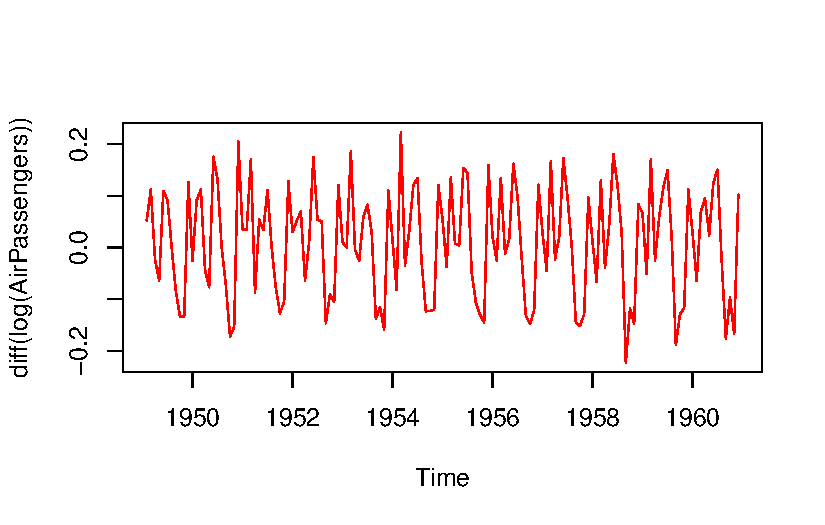
\includegraphics{data_analysis_files/figure-pdf/unnamed-chunk-5-6.pdf}

}

\end{figure}

\begin{Shaded}
\begin{Highlighting}[]
\CommentTok{\# çoklu zaman serisi}
\NormalTok{ts }\OtherTok{\textless{}{-}} \FunctionTok{ts}\NormalTok{(}\FunctionTok{rnorm}\NormalTok{(}\FunctionTok{length}\NormalTok{(AirPassengers),}\DecValTok{250}\NormalTok{,}\DecValTok{100}\NormalTok{),}\AttributeTok{start =} \FunctionTok{c}\NormalTok{(}\DecValTok{1949}\NormalTok{,}\DecValTok{1}\NormalTok{),}\AttributeTok{frequency=}\DecValTok{12}\NormalTok{)}
\NormalTok{ts}
\end{Highlighting}
\end{Shaded}

\begin{verbatim}
             Jan         Feb         Mar         Apr         May         Jun
1949 114.9785126 181.2588533 185.9624739 222.4016412 284.0819392 299.6452379
1950 295.9431328 386.2106622 150.3279123 450.4012491 223.5465728 389.4714735
1951   0.5901196 238.7657506 274.0145918 320.9399230 196.5535479 328.6007260
1952 420.9429550   0.2866262 211.6132475 320.7560123 348.2397101 337.5951564
1953 262.5659930 252.7844027 132.1700414 304.2418397 367.1954606  96.4243469
1954 283.3054914 182.2897083 149.9399407 362.7138318  88.2051765 267.1052695
1955 322.2757233 284.0537642 290.6584213 241.6123682 362.9114049 446.6970445
1956 456.7314627 255.3616024 273.9488173 204.4390879 269.1385540 252.9697011
1957 -97.8114931 205.3477564 130.0610969 342.9982791 140.8509562 318.2385029
1958 370.7304423 240.7963474 115.5474500 348.5575815 179.2996601 118.0043638
1959 335.2937483 270.7994137  76.9429500 267.3631493 318.9326698  70.6506276
1960 323.6158989 306.7548894 233.3712234 292.3662143 362.7983645 183.4513671
             Jul         Aug         Sep         Oct         Nov         Dec
1949 295.3858349 210.5839730 271.6193590 185.4910752 177.0307562 187.7773867
1950 346.4820860 159.8986438 249.6084907 100.2041371 170.7333034 270.1301413
1951  74.5846951 334.2802033 349.6167237 130.2974884 223.0300064 275.9585927
1952 230.1479569 207.0988687 341.0484750 190.2352123 187.1040308 264.8670060
1953 428.6798941 102.3010714 -10.4814508 241.7499327 133.0080524 309.1979283
1954 127.4857803 153.1310611 277.6187629 415.7383637 308.6762438 189.5626531
1955 190.2995666 177.5334586 360.8715000  66.5726655 186.1911220 317.6853889
1956  44.3065889 143.3656204 324.4376477 147.7007719 409.0344432 105.1203362
1957 290.0420300 108.3164761 146.2702750 216.0359133 271.9366677 303.1000348
1958 196.6212858 214.2479858 255.2216316 293.1790676 157.8841464 269.8625656
1959 288.9146152 195.0214290 275.7739556 380.8699593 151.4814280 347.1643688
1960 226.0708048 221.6219232 247.1360022 202.8255117 135.5975188 206.0298643
\end{verbatim}

\begin{Shaded}
\begin{Highlighting}[]
\FunctionTok{plot}\NormalTok{(AirPassengers,}\AttributeTok{type =} \StringTok{"l"}\NormalTok{,}\AttributeTok{col =} \StringTok{"red"}\NormalTok{)}
\FunctionTok{lines}\NormalTok{(ts, }\AttributeTok{type =} \StringTok{"l"}\NormalTok{, }\AttributeTok{col =} \StringTok{"blue"}\NormalTok{)}
\end{Highlighting}
\end{Shaded}

\begin{figure}[H]

{\centering 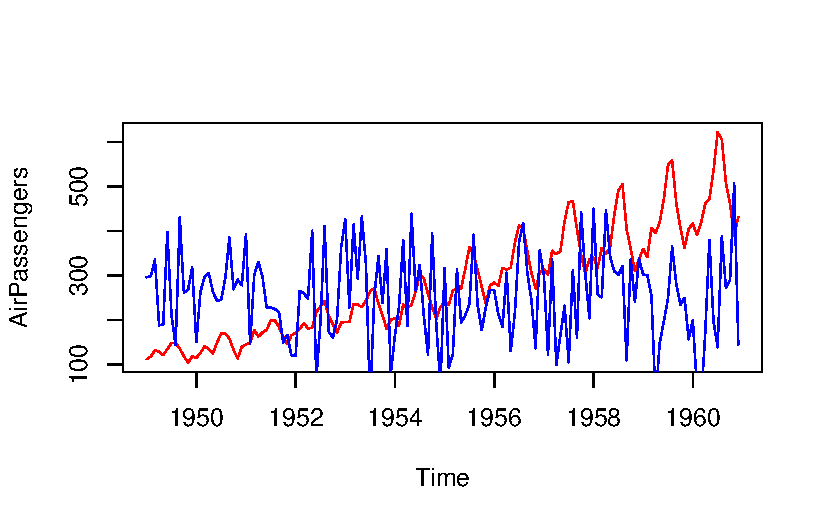
\includegraphics{data_analysis_files/figure-pdf/unnamed-chunk-5-7.pdf}

}

\end{figure}

\begin{Shaded}
\begin{Highlighting}[]
\CommentTok{\# yüzde değişim}
\NormalTok{growth }\OtherTok{\textless{}{-}}\NormalTok{ AirPassengers}\SpecialCharTok{/}\NormalTok{stats}\SpecialCharTok{::}\FunctionTok{lag}\NormalTok{(AirPassengers,}\SpecialCharTok{{-}}\DecValTok{1}\NormalTok{)}\SpecialCharTok{*}\DecValTok{100{-}100}
\NormalTok{growth}
\end{Highlighting}
\end{Shaded}

\begin{verbatim}
             Jan         Feb         Mar         Apr         May         Jun
1949               5.3571429  11.8644068  -2.2727273  -6.2015504  11.5702479
1950  -2.5423729   9.5652174  11.9047619  -4.2553191  -7.4074074  19.2000000
1951   3.5714286   3.4482759  18.6666667  -8.4269663   5.5214724   3.4883721
1952   3.0120482   5.2631579   7.2222222  -6.2176166   1.1049724  19.1256831
1953   1.0309278   0.0000000  20.4081633  -0.4237288  -2.5531915   6.1135371
1954   1.4925373  -7.8431373  25.0000000  -3.4042553   3.0837004  12.8205128
1955   5.6768559  -3.7190083  14.5922747   0.7490637   0.3717472  16.6666667
1956   2.1582734  -2.4647887  14.4404332  -1.2618297   1.5974441  17.6100629
1957   2.9411765  -4.4444444  18.2724252  -2.2471910   2.0114943  18.8732394
1958   1.1904762  -6.4705882  13.8364780  -3.8674033   4.3103448  19.8347107
1959   6.8249258  -5.0000000  18.7134503  -2.4630542   6.0606061  12.3809524
1960   2.9629630  -6.2350120   7.1611253  10.0238663   2.3861171  13.3474576
             Jul         Aug         Sep         Oct         Nov         Dec
1949   9.6296296   0.0000000  -8.1081081 -12.5000000 -12.6050420  13.4615385
1950  14.0939597   0.0000000  -7.0588235 -15.8227848 -14.2857143  22.8070175
1951  11.7977528   0.0000000  -7.5376884 -11.9565217  -9.8765432  13.6986301
1952   5.5045872   5.2173913 -13.6363636  -8.6124402  -9.9476440  12.7906977
1953   8.6419753   3.0303030 -12.8676471 -10.9704641 -14.6919431  11.6666667
1954  14.3939394  -2.9801325 -11.6040956 -11.5830116 -11.3537118  12.8078818
1955  15.5555556  -4.6703297 -10.0864553 -12.1794872 -13.5036496  17.2995781
1956  10.4278075  -1.9370460 -12.3456790 -13.8028169 -11.4379085  12.9151292
1957  10.1895735   0.4301075 -13.4903640 -14.1089109 -12.1037464  10.1639344
1958  12.8735632   2.8513238 -20.0000000 -11.1386139 -13.6490251   8.7096774
1959  16.1016949   2.0072993 -17.1735242 -12.0950324 -11.0565111  11.8784530
1960  16.2616822  -2.5723473 -16.1716172  -9.2519685 -15.4013015  10.7692308
\end{verbatim}

\begin{Shaded}
\begin{Highlighting}[]
\FunctionTok{plot}\NormalTok{(growth,}\AttributeTok{type =} \StringTok{"l"}\NormalTok{, }\AttributeTok{col =} \StringTok{"red"}\NormalTok{)}
\end{Highlighting}
\end{Shaded}

\begin{figure}[H]

{\centering 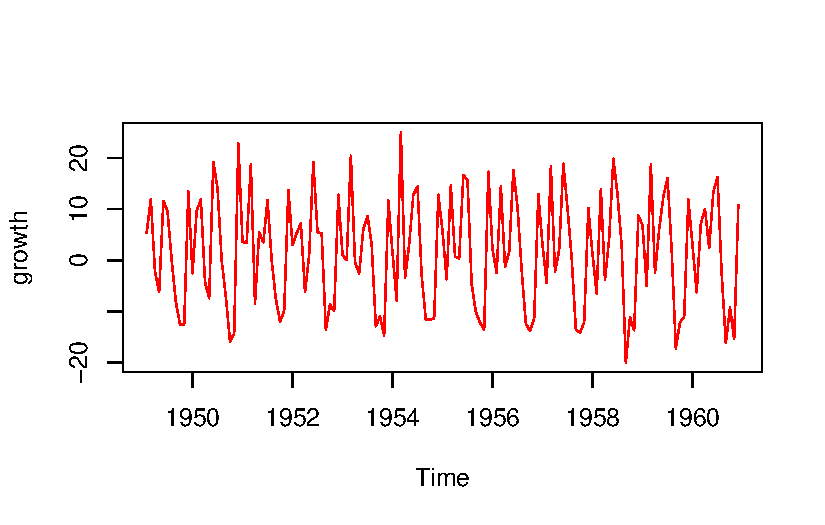
\includegraphics{data_analysis_files/figure-pdf/unnamed-chunk-5-8.pdf}

}

\end{figure}

\hypertarget{veri-analizi-bazux131-paketler}{%
\section*{Veri Analizi Bazı
Paketler}\label{veri-analizi-bazux131-paketler}}
\addcontentsline{toc}{section}{Veri Analizi Bazı Paketler}

\markright{Veri Analizi Bazı Paketler}

Veri analizi için
\href{https://cran.r-project.org/web/packages/skimr/vignettes/skimr.html}{skimr}
paketi de kullanılabilir. \textbf{\texttt{skimr}}, R programlama dilinde
veri setlerinin hızlı bir şekilde özetlenmesini sağlayan bir pakettir.
Veri setlerinin yapısını, özelliklerini ve bazı istatistiksel özetlerini
görsel ve açıklayıcı bir şekilde sunar. Bu paket, veri keşfi aşamasında
veri setinin genel özelliklerini anlamak için kullanılır.

\textbf{\texttt{skimr}} paketi, veri setinizdeki değişkenlerin türlerine
göre istatistiksel özetler sunar. Örneğin, sayısal değişkenler için
merkezi eğilim ölçüleri (ortalama, medyan), dağılım (standart sapma,
min-max değerleri), faktör değişkenleri için sınıf sayısı, en sık
rastlanan sınıf ve eksik veri durumları gibi bilgileri sunar.

Bu paket, veri setinin yapısını hızlıca anlamak ve önemli özelliklerini
keşfetmek için kullanılır. Özellikle veri setlerinin keşfedilmesi,
temizlenmesi ve analiz edilmesi aşamalarında oldukça faydalıdır. Bu,
veri analiz sürecinde veriye daha derinlemesine bakmayı ve hangi analiz
tekniklerinin kullanılacağına dair daha iyi bir anlayış geliştirmeyi
sağlar.

Bunun yanında, \href{https://modelsummary.com/}{modelsummary} paketi de,
R programlama dili için geliştirilmiş olan bir pakettir ve istatistiksel
modellerin özetlenmesi, karşılaştırılması ve görselleştirilmesi için
kullanılır. Bu paket, farklı türdeki modellerin çıktılarını
standartlaştırarak, bunları karşılaştırmak ve analiz etmek için
kullanıcıya kolaylık sağlar.

Bu paket genellikle doğrusal regresyon, lojistik regresyon, karar
ağaçları, destek vektör makineleri gibi çeşitli istatistiksel ve makine
öğrenimi modellerinin özet istatistiklerini, katsayılarını, belirlilik
ölçülerini, hata ölçümlerini ve diğer önemli çıktıları sunar. Bunların
yanı sıra, çıktıları tablolar halinde gösterir ve görselleştirmeler
yaparak model performansını karşılaştırmak için grafikler oluşturabilir.

Bu paket, araştırmacılar, veri bilimcileri veya istatistikçilerin farklı
modelleri anlamak, karşılaştırmak ve raporlamak için verimli bir araç
sunar. Model sonuçlarını görselleştirme ve karşılaştırma açısından
kullanışlıdır. Paket, model özetlerinin ötesinde, veri kümesine genel
bakış, korelasyon matrisleri, (çok seviyeli) çapraz tablolar ve denge
tabloları gibi son derece esnek veri özet tabloları üretmek için bir
dizi araç da içerir.

\begin{Shaded}
\begin{Highlighting}[]
\CommentTok{\# Paketin birkaç özelliğine bakalım}

\FunctionTok{library}\NormalTok{(modelsummary)}

\CommentTok{\# kategorik verilere hızlı bir bakış}
\FunctionTok{datasummary\_skim}\NormalTok{(mpg, }\StringTok{"categorical"}\NormalTok{)}
\end{Highlighting}
\end{Shaded}

\begin{table}
\centering
\begin{tabular}[t]{llrr}
\toprule
  &    & N & \%\\
\midrule
manufacturer & audi & 18 & \num{7.7}\\
 & chevrolet & 19 & \num{8.1}\\
 & dodge & 37 & \num{15.8}\\
 & ford & 25 & \num{10.7}\\
 & honda & 9 & \num{3.8}\\
 & hyundai & 14 & \num{6.0}\\
 & jeep & 8 & \num{3.4}\\
 & land rover & 4 & \num{1.7}\\
 & lincoln & 3 & \num{1.3}\\
 & mercury & 4 & \num{1.7}\\
 & nissan & 13 & \num{5.6}\\
 & pontiac & 5 & \num{2.1}\\
 & subaru & 14 & \num{6.0}\\
 & toyota & 34 & \num{14.5}\\
 & volkswagen & 27 & \num{11.5}\\
model & 4runner 4wd & 6 & \num{2.6}\\
 & a4 & 7 & \num{3.0}\\
 & a4 quattro & 8 & \num{3.4}\\
 & a6 quattro & 3 & \num{1.3}\\
 & altima & 6 & \num{2.6}\\
 & c1500 suburban 2wd & 5 & \num{2.1}\\
 & camry & 7 & \num{3.0}\\
 & camry solara & 7 & \num{3.0}\\
 & caravan 2wd & 11 & \num{4.7}\\
 & civic & 9 & \num{3.8}\\
 & corolla & 5 & \num{2.1}\\
 & corvette & 5 & \num{2.1}\\
 & dakota pickup 4wd & 9 & \num{3.8}\\
 & durango 4wd & 7 & \num{3.0}\\
 & expedition 2wd & 3 & \num{1.3}\\
 & explorer 4wd & 6 & \num{2.6}\\
 & f150 pickup 4wd & 7 & \num{3.0}\\
 & forester awd & 6 & \num{2.6}\\
 & grand cherokee 4wd & 8 & \num{3.4}\\
 & grand prix & 5 & \num{2.1}\\
 & gti & 5 & \num{2.1}\\
 & impreza awd & 8 & \num{3.4}\\
 & jetta & 9 & \num{3.8}\\
 & k1500 tahoe 4wd & 4 & \num{1.7}\\
 & land cruiser wagon 4wd & 2 & \num{0.9}\\
 & malibu & 5 & \num{2.1}\\
 & maxima & 3 & \num{1.3}\\
 & mountaineer 4wd & 4 & \num{1.7}\\
 & mustang & 9 & \num{3.8}\\
 & navigator 2wd & 3 & \num{1.3}\\
 & new beetle & 6 & \num{2.6}\\
 & passat & 7 & \num{3.0}\\
 & pathfinder 4wd & 4 & \num{1.7}\\
 & ram 1500 pickup 4wd & 10 & \num{4.3}\\
 & range rover & 4 & \num{1.7}\\
 & sonata & 7 & \num{3.0}\\
 & tiburon & 7 & \num{3.0}\\
 & toyota tacoma 4wd & 7 & \num{3.0}\\
trans & auto(av) & 5 & \num{2.1}\\
 & auto(l3) & 2 & \num{0.9}\\
 & auto(l4) & 83 & \num{35.5}\\
 & auto(l5) & 39 & \num{16.7}\\
 & auto(l6) & 6 & \num{2.6}\\
 & auto(s4) & 3 & \num{1.3}\\
 & auto(s5) & 3 & \num{1.3}\\
 & auto(s6) & 16 & \num{6.8}\\
 & manual(m5) & 58 & \num{24.8}\\
 & manual(m6) & 19 & \num{8.1}\\
drv & 4 & 103 & \num{44.0}\\
 & f & 106 & \num{45.3}\\
 & r & 25 & \num{10.7}\\
fl & c & 1 & \num{0.4}\\
 & d & 5 & \num{2.1}\\
 & e & 8 & \num{3.4}\\
 & p & 52 & \num{22.2}\\
 & r & 168 & \num{71.8}\\
class & 2seater & 5 & \num{2.1}\\
 & compact & 47 & \num{20.1}\\
 & midsize & 41 & \num{17.5}\\
 & minivan & 11 & \num{4.7}\\
 & pickup & 33 & \num{14.1}\\
 & subcompact & 35 & \num{15.0}\\
 & suv & 62 & \num{26.5}\\
\bottomrule
\end{tabular}
\end{table}

\begin{Shaded}
\begin{Highlighting}[]
\CommentTok{\# nümerik verilere hızlı bir bakış}
\FunctionTok{datasummary\_skim}\NormalTok{(mpg, }\StringTok{"numeric"}\NormalTok{)}
\end{Highlighting}
\end{Shaded}

\begin{table}
\centering
\begin{tabular}[t]{lrrrrrrr>{}r}
\toprule
  & Unique (\#) & Missing (\%) & Mean & SD & Min & Median & Max &   \\
\midrule
displ & 35 & 0 & \num{3.5} & \num{1.3} & \num{1.6} & \num{3.3} & \num{7.0} & 
\includegraphics[width=0.67in, height=0.17in]{D:/Akademi ve Veri Bilimi/Data Science/Github/r-book-tr/data_analysis_files/figure-latex/hist_45389a21f8a.pdf}\\
year & 2 & 0 & \num{2003.5} & \num{4.5} & \num{1999.0} & \num{2003.5} & \num{2008.0} & 
\includegraphics[width=0.67in, height=0.17in]{D:/Akademi ve Veri Bilimi/Data Science/Github/r-book-tr/data_analysis_files/figure-latex/hist_453851d53637.pdf}\\
cyl & 4 & 0 & \num{5.9} & \num{1.6} & \num{4.0} & \num{6.0} & \num{8.0} & 
\includegraphics[width=0.67in, height=0.17in]{D:/Akademi ve Veri Bilimi/Data Science/Github/r-book-tr/data_analysis_files/figure-latex/hist_4538579d168f.pdf}\\
cty & 21 & 0 & \num{16.9} & \num{4.3} & \num{9.0} & \num{17.0} & \num{35.0} & 
\includegraphics[width=0.67in, height=0.17in]{D:/Akademi ve Veri Bilimi/Data Science/Github/r-book-tr/data_analysis_files/figure-latex/hist_4538b5a25b9.pdf}\\
hwy & 27 & 0 & \num{23.4} & \num{6.0} & \num{12.0} & \num{24.0} & \num{44.0} & 
\includegraphics[width=0.67in, height=0.17in]{D:/Akademi ve Veri Bilimi/Data Science/Github/r-book-tr/data_analysis_files/figure-latex/hist_45383e5178e3.pdf}\\
\bottomrule
\end{tabular}
\end{table}

\bookmarksetup{startatroot}

\hypertarget{ggplot2-ile-veri-guxf6rselleux15ftirme}{%
\chapter*{ggplot2 ile Veri
Görselleştirme}\label{ggplot2-ile-veri-guxf6rselleux15ftirme}}
\addcontentsline{toc}{chapter}{ggplot2 ile Veri Görselleştirme}

\markboth{ggplot2 ile Veri Görselleştirme}{ggplot2 ile Veri
Görselleştirme}

\begin{figure}

{\centering 
\includegraphics[width=4.4375in,height=3.20833in]{images/ggplot2.png}

}

\end{figure}

Bu bölümde ggplot2 paketi ile verilerin nasıl görselleştirldiğine
bakacağız. ggplot2 grafiklerin dil bilgisi \textbf{(grammar of
graphics)} prensiplerini temel alarak oluşturulmuştur. Bu prensiplere
göre her grafik aynı parçalardan oluşturulabilir: bir veri seti,
koordinat sistemi, ve ``\textbf{\texttt{geom}}''lar - veri noktalarını
temsil eden görsel işaretler.

ggplot2 ile veri görselleştirebilmemiz için önce grafik yapısını iyi
tanımamız gerekiyor. Yatay eksen x ekseni, dikey eksen ise y ekseni
olarak kabul ediliyor. Veri görselleştirmede
\textbf{\texttt{ggplot}}\texttt{()} fonksiyonunu kullanıyoruz. ggplot()
fonksiyonu içinde veri seti ismi ve \textbf{\texttt{aes}}\texttt{()}
adlı estetik argümanına yatay ve dikey eksende kullanacağımız
değişkenler (sütun isimleri) ile yer veriyoruz. Sonrasında, tercih
edeceğimiz grafik tipine göre, \textbf{\texttt{geom}} fonksiyonlarından
birini kullanacağız. Sıklıkla kullanılan geom fonksiyonları şunlardır:

\begin{itemize}
\item
  Nokta grafiği için \texttt{geom\_point()}
\item
  Çubuk veya sütun grafik için \texttt{geom\_col()} ve
  \texttt{geom\_bar()}
\item
  Çizgi grafiği için \texttt{geom\_line()}
\item
  Histogram grafiği için \texttt{geom\_histogram()}
\item
  Boxplot grafiği için \texttt{geom\_boxplot()}
\end{itemize}

\hypertarget{sauxe7ux131lux131m-grafikleri}{%
\section*{Saçılım Grafikleri}\label{sauxe7ux131lux131m-grafikleri}}
\addcontentsline{toc}{section}{Saçılım Grafikleri}

\markright{Saçılım Grafikleri}

Saçılım grafiği, genellikle fizik ve istatistik gibi bilimlerde
kullanılan bir grafik türüdür. Saçılım grafiği, iki değişken arasındaki
ilişkiyi görsel olarak göstermek için kullanılır. Bir eksende bir
değişkenin değerleri, diğer eksende ise diğer değişkenin değerleri yer
alır, ve her veri noktası bu iki değişkenin birleşimini temsil eder.
Saçılım grafiği, veri noktalarının dağılımını, yoğunluklarını, odaklanma
noktalarını ve olası eğilimleri anlamak için kullanılır. Bu grafik, veri
setindeki aykırı değerleri tespit etmek, iki değişken arasındaki
ilişkiyi değerlendirmek ve korelasyonu görsel olarak incelemek için
oldukça kullanışlıdır.

Saçılım grafiği kullanarak, iki değişken arasındaki ilişkinin doğası
hakkında bilgi edinebilirsiniz. Örneğin, pozitif bir korelasyon varsa,
veri noktaları genellikle yukarı doğru bir eğilim gösterirken, negatif
bir korelasyon varsa, veri noktaları genellikle aşağı doğru bir eğilim
gösterir. Korelasyon olmaması durumunda ise veri noktaları dağınık bir
şekilde yayılmış olur. Saçılım grafiği, istatistiksel analizlerde veri
keşfi yapmak ve ilişkileri anlamak için önemli bir araçtır.

\begin{Shaded}
\begin{Highlighting}[]
\FunctionTok{library}\NormalTok{(ggplot2)}
\FunctionTok{library}\NormalTok{(dplyr)}
\end{Highlighting}
\end{Shaded}

\begin{verbatim}

Attaching package: 'dplyr'
\end{verbatim}

\begin{verbatim}
The following objects are masked from 'package:stats':

    filter, lag
\end{verbatim}

\begin{verbatim}
The following objects are masked from 'package:base':

    intersect, setdiff, setequal, union
\end{verbatim}

\begin{Shaded}
\begin{Highlighting}[]
\CommentTok{\# Bir önceki bölümde üretilen yeni değişkenleri mpg veri setine yine ekleyelim.}

\CommentTok{\# litre başına km hesaplama}
\NormalTok{galonmil\_to\_ltkm }\OtherTok{\textless{}{-}} \ControlFlowTok{function}\NormalTok{(x)\{}
  
\NormalTok{  km }\OtherTok{\textless{}{-}}\NormalTok{ x }\SpecialCharTok{*} \FloatTok{1.609}\SpecialCharTok{/}\FloatTok{3.79}
  \FunctionTok{return}\NormalTok{(km)}
\NormalTok{\}}

\NormalTok{df }\OtherTok{\textless{}{-}}\NormalTok{ mpg}
\NormalTok{df}\SpecialCharTok{$}\NormalTok{cty\_ltkm }\OtherTok{\textless{}{-}} \FunctionTok{galonmil\_to\_ltkm}\NormalTok{(df}\SpecialCharTok{$}\NormalTok{cty)}
\NormalTok{df}\SpecialCharTok{$}\NormalTok{hwy\_ltkm }\OtherTok{\textless{}{-}} \FunctionTok{galonmil\_to\_ltkm}\NormalTok{(df}\SpecialCharTok{$}\NormalTok{hwy)}

\NormalTok{p1 }\OtherTok{\textless{}{-}} \FunctionTok{ggplot}\NormalTok{(df,}\FunctionTok{aes}\NormalTok{(}\AttributeTok{x=}\NormalTok{displ,}\AttributeTok{y=}\NormalTok{cty\_ltkm)) }\SpecialCharTok{+}
  \FunctionTok{geom\_point}\NormalTok{(}\AttributeTok{size=}\DecValTok{2}\NormalTok{,}\AttributeTok{color=}\StringTok{"red"}\NormalTok{)}
\NormalTok{p1}
\end{Highlighting}
\end{Shaded}

\begin{figure}[H]

{\centering 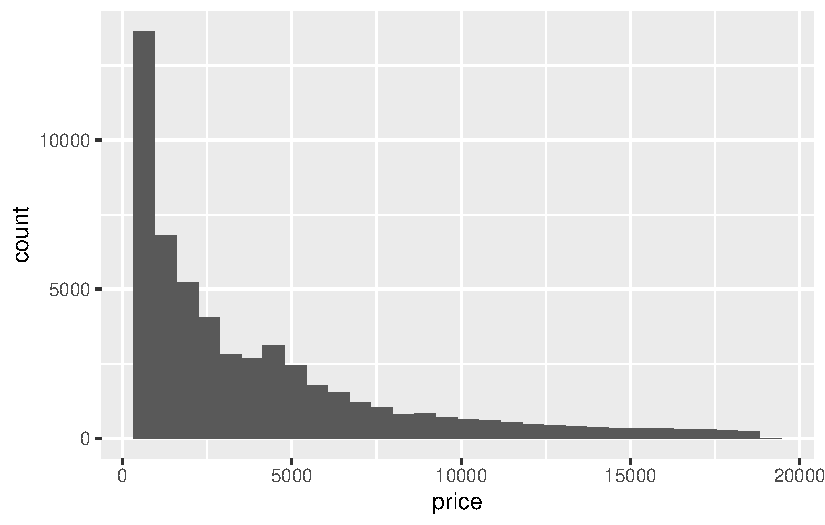
\includegraphics{ggplot2_files/figure-pdf/unnamed-chunk-1-1.pdf}

}

\end{figure}

\begin{Shaded}
\begin{Highlighting}[]
\CommentTok{\# gruplar düzeyinde grafiği çizdirme}
\NormalTok{p2 }\OtherTok{\textless{}{-}} \FunctionTok{ggplot}\NormalTok{(df,}\FunctionTok{aes}\NormalTok{(}\AttributeTok{x=}\NormalTok{displ,}\AttributeTok{y=}\NormalTok{cty\_ltkm,}\AttributeTok{colour=}\FunctionTok{as.factor}\NormalTok{(year))) }\SpecialCharTok{+}
  \FunctionTok{geom\_point}\NormalTok{(}\AttributeTok{size=}\DecValTok{2}\NormalTok{) }\SpecialCharTok{+}
  \CommentTok{\# grafiğe başlık ekleme}
  \FunctionTok{ggtitle}\NormalTok{(}\StringTok{"Motor Hacmi ve Yakıt Tüketimi Saçılım Grafiği"}\NormalTok{) }\SpecialCharTok{+}
  \CommentTok{\#eksenleri isimlendirme}
  \FunctionTok{xlab}\NormalTok{(}\StringTok{"Motor Hacmi"}\NormalTok{) }\SpecialCharTok{+} 
  \FunctionTok{ylab}\NormalTok{(}\StringTok{"Yakıt Tüketimi"}\NormalTok{)}\SpecialCharTok{+}
  \FunctionTok{theme\_bw}\NormalTok{() }\SpecialCharTok{+} \CommentTok{\# tema değiştirme}
  \FunctionTok{theme}\NormalTok{(}\AttributeTok{legend.position =} \StringTok{"bottom"}\NormalTok{,  }\CommentTok{\# gruplama değişkeninin poziyounun değiştirme}
        \AttributeTok{plot.title =} \FunctionTok{element\_text}\NormalTok{(}\AttributeTok{face =} \StringTok{"bold"}\NormalTok{), }\CommentTok{\# kalın başlık}
        \AttributeTok{legend.title =} \FunctionTok{element\_blank}\NormalTok{()) }\CommentTok{\# grup başlığını kaldırma}
\NormalTok{p2  }
\end{Highlighting}
\end{Shaded}

\begin{figure}[H]

{\centering 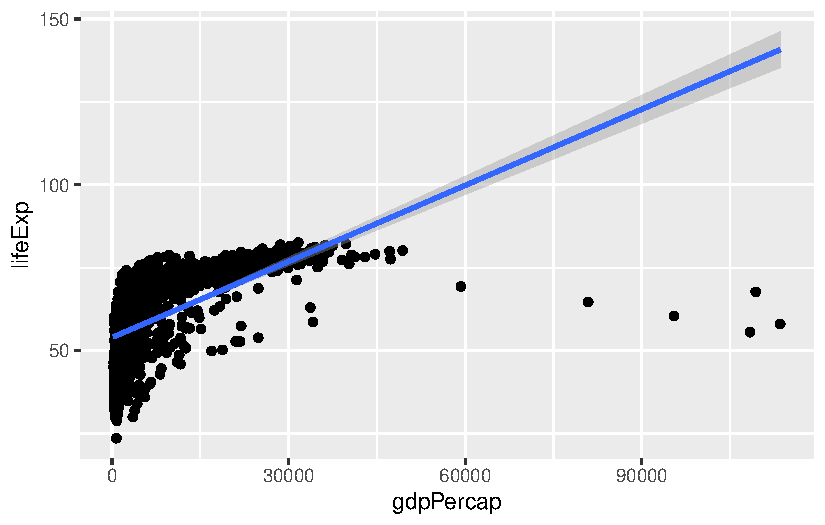
\includegraphics{ggplot2_files/figure-pdf/unnamed-chunk-1-2.pdf}

}

\end{figure}

\begin{Shaded}
\begin{Highlighting}[]
\FunctionTok{ggplot}\NormalTok{(df,}\FunctionTok{aes}\NormalTok{(}\AttributeTok{x=}\NormalTok{displ,}\AttributeTok{y=}\NormalTok{cty\_ltkm)) }\SpecialCharTok{+}
  \FunctionTok{geom\_point}\NormalTok{(}\FunctionTok{aes}\NormalTok{(}\AttributeTok{size=}\FunctionTok{factor}\NormalTok{(cyl)),}\AttributeTok{color=}\StringTok{"red"}\NormalTok{)}
\end{Highlighting}
\end{Shaded}

\begin{figure}[H]

{\centering 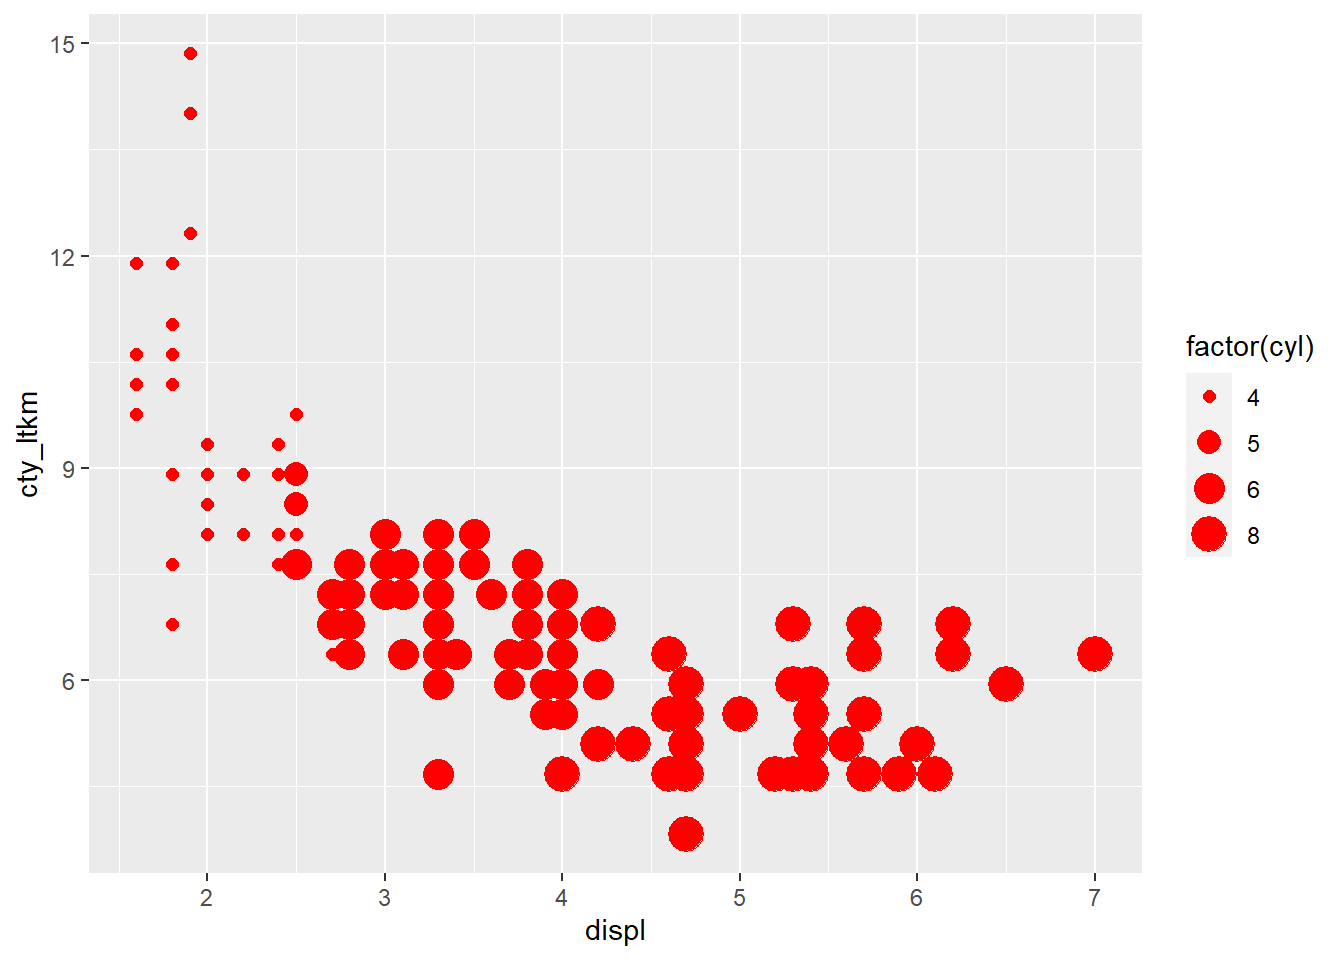
\includegraphics{ggplot2_files/figure-pdf/unnamed-chunk-1-3.pdf}

}

\end{figure}

\begin{Shaded}
\begin{Highlighting}[]
\CommentTok{\# grafiğe model eğrisi ekleme}
\NormalTok{p1 }\SpecialCharTok{+} \FunctionTok{geom\_smooth}\NormalTok{(}\AttributeTok{method =}\NormalTok{ lm, }\AttributeTok{se =} \ConstantTok{TRUE}\NormalTok{)}
\end{Highlighting}
\end{Shaded}

\begin{verbatim}
`geom_smooth()` using formula = 'y ~ x'
\end{verbatim}

\begin{figure}[H]

{\centering 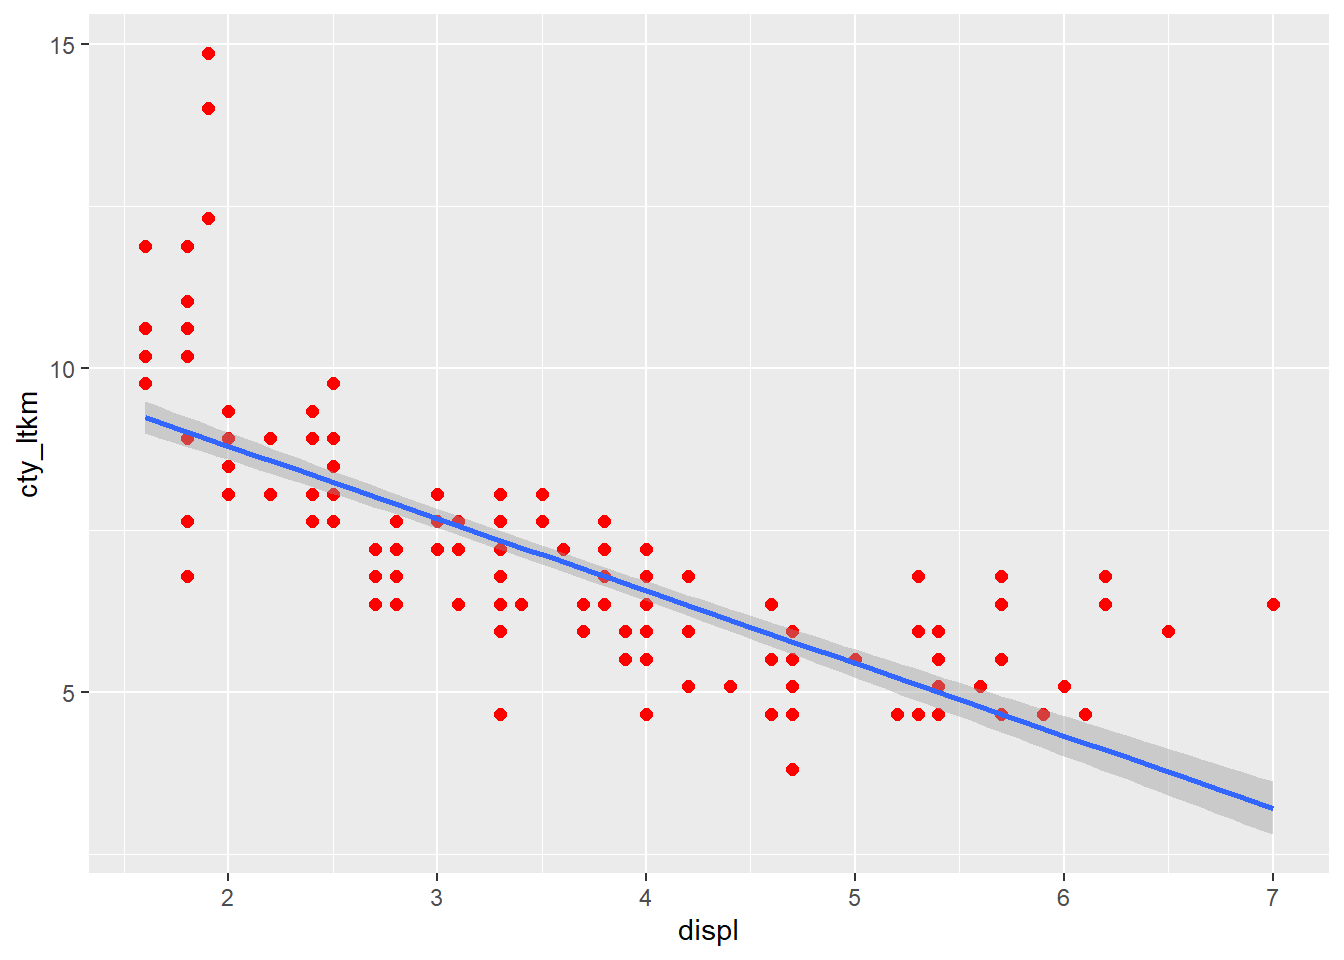
\includegraphics{ggplot2_files/figure-pdf/unnamed-chunk-1-4.pdf}

}

\end{figure}

\begin{Shaded}
\begin{Highlighting}[]
\NormalTok{p1 }\SpecialCharTok{+} \FunctionTok{geom\_smooth}\NormalTok{(}\AttributeTok{method =}\NormalTok{ loess, }\AttributeTok{se =} \ConstantTok{TRUE}\NormalTok{)}
\end{Highlighting}
\end{Shaded}

\begin{verbatim}
`geom_smooth()` using formula = 'y ~ x'
\end{verbatim}

\begin{figure}[H]

{\centering 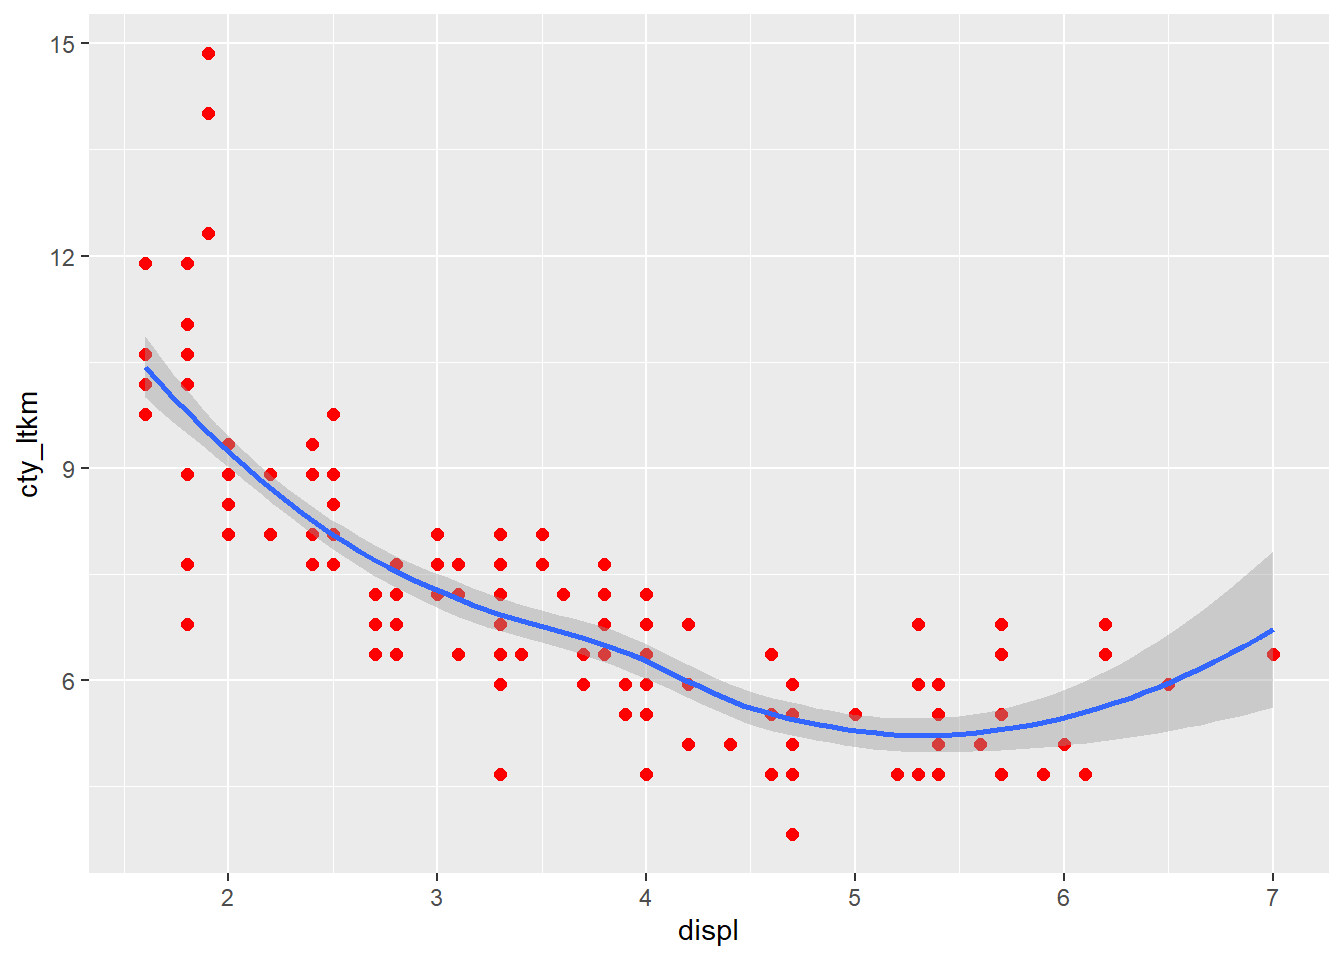
\includegraphics{ggplot2_files/figure-pdf/unnamed-chunk-1-5.pdf}

}

\end{figure}

\begin{Shaded}
\begin{Highlighting}[]
\CommentTok{\# grup düzeyinde model eğrileri ve saçılım grafiği}
\NormalTok{p3 }\OtherTok{\textless{}{-}}\NormalTok{ df }\SpecialCharTok{\%\textgreater{}\%} 
  \FunctionTok{ggplot}\NormalTok{(}\FunctionTok{aes}\NormalTok{(}\AttributeTok{x=}\NormalTok{displ,}\AttributeTok{y=}\NormalTok{cty\_ltkm,}\AttributeTok{color=}\FunctionTok{as.factor}\NormalTok{(cyl))) }\SpecialCharTok{+}
  \FunctionTok{geom\_point}\NormalTok{()  }\SpecialCharTok{+} 
  \FunctionTok{geom\_smooth}\NormalTok{(}\AttributeTok{method =}\NormalTok{ lm, }\AttributeTok{se =} \ConstantTok{TRUE}\NormalTok{)}
\NormalTok{p3}
\end{Highlighting}
\end{Shaded}

\begin{verbatim}
`geom_smooth()` using formula = 'y ~ x'
\end{verbatim}

\begin{figure}[H]

{\centering 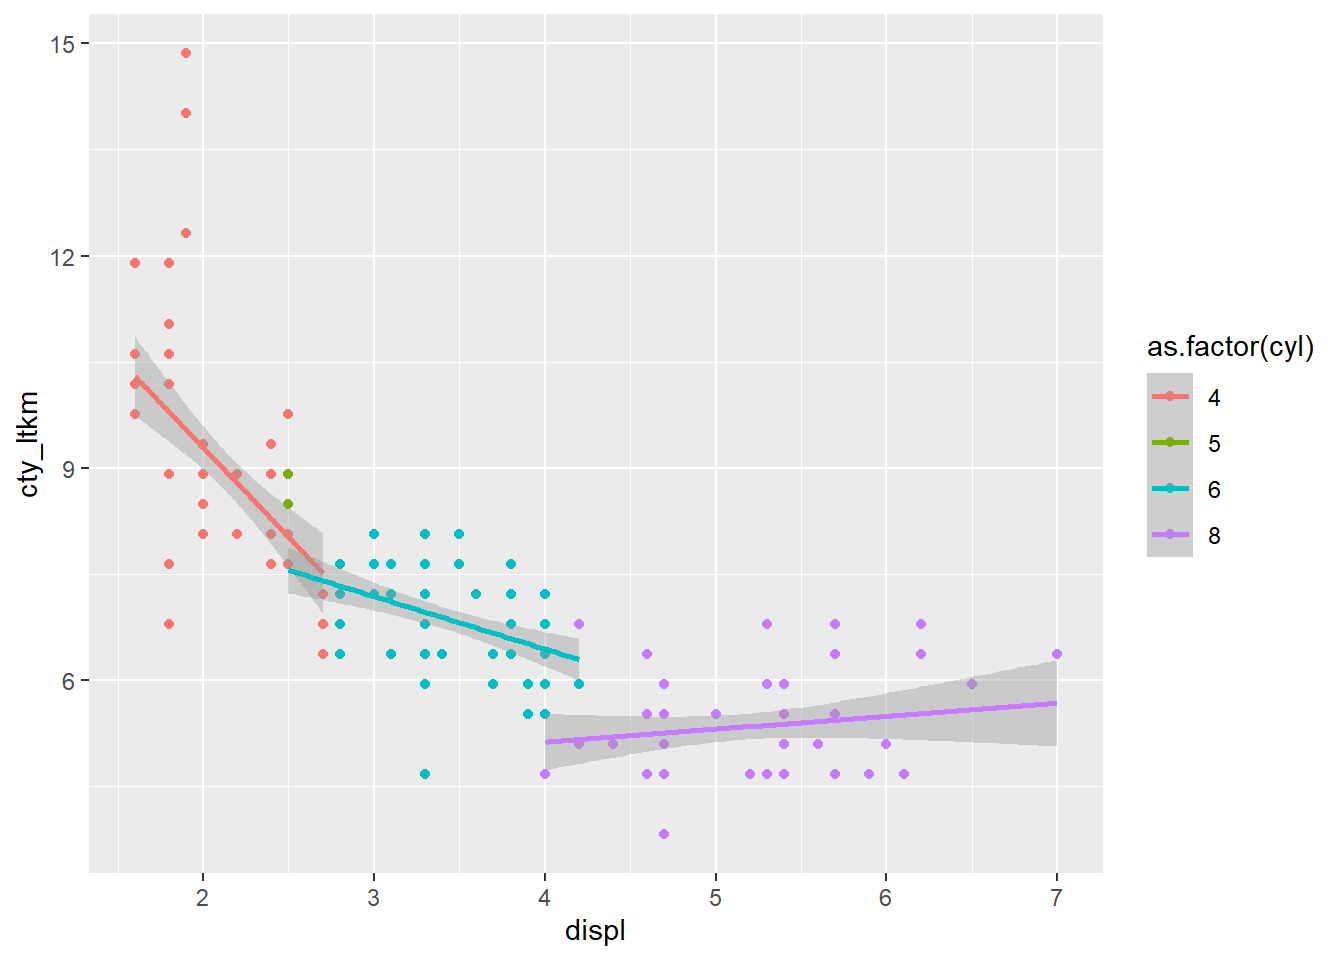
\includegraphics{ggplot2_files/figure-pdf/unnamed-chunk-1-6.pdf}

}

\end{figure}

\begin{Shaded}
\begin{Highlighting}[]
\CommentTok{\# grup ve yıl düzeyinde model eğrileri ve saçılım grafiği}
\NormalTok{p3 }\SpecialCharTok{+} \FunctionTok{facet\_wrap}\NormalTok{(}\SpecialCharTok{\textasciitilde{}}\NormalTok{ year)}
\end{Highlighting}
\end{Shaded}

\begin{verbatim}
`geom_smooth()` using formula = 'y ~ x'
\end{verbatim}

\begin{figure}[H]

{\centering 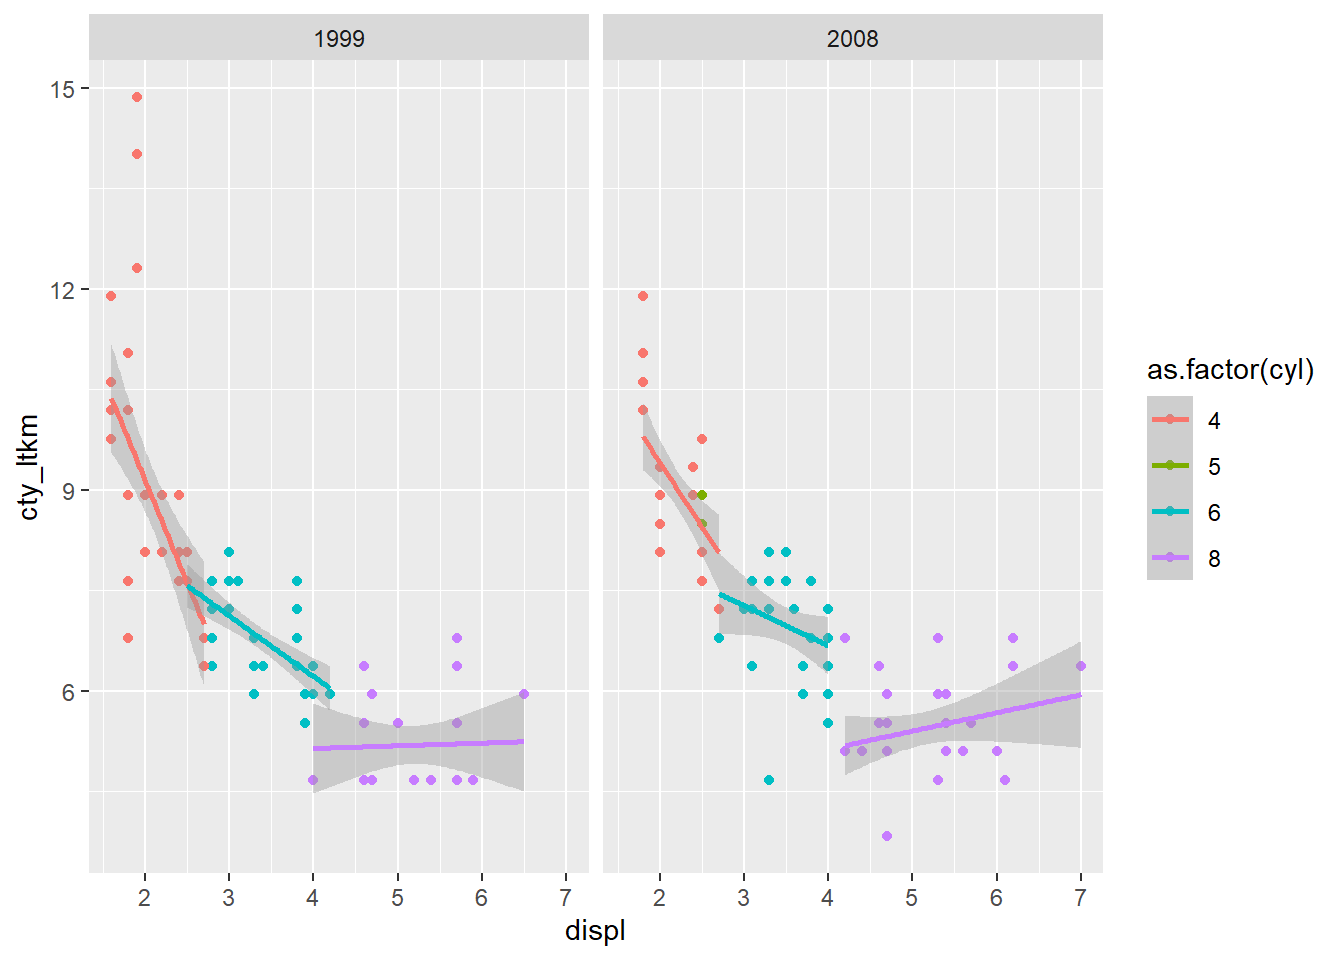
\includegraphics{ggplot2_files/figure-pdf/unnamed-chunk-1-7.pdf}

}

\end{figure}

\begin{Shaded}
\begin{Highlighting}[]
\NormalTok{p3 }\SpecialCharTok{+} \FunctionTok{facet\_wrap}\NormalTok{(}\SpecialCharTok{\textasciitilde{}}\NormalTok{ year}\SpecialCharTok{+}\NormalTok{drv)}
\end{Highlighting}
\end{Shaded}

\begin{verbatim}
`geom_smooth()` using formula = 'y ~ x'
\end{verbatim}

\begin{figure}[H]

{\centering 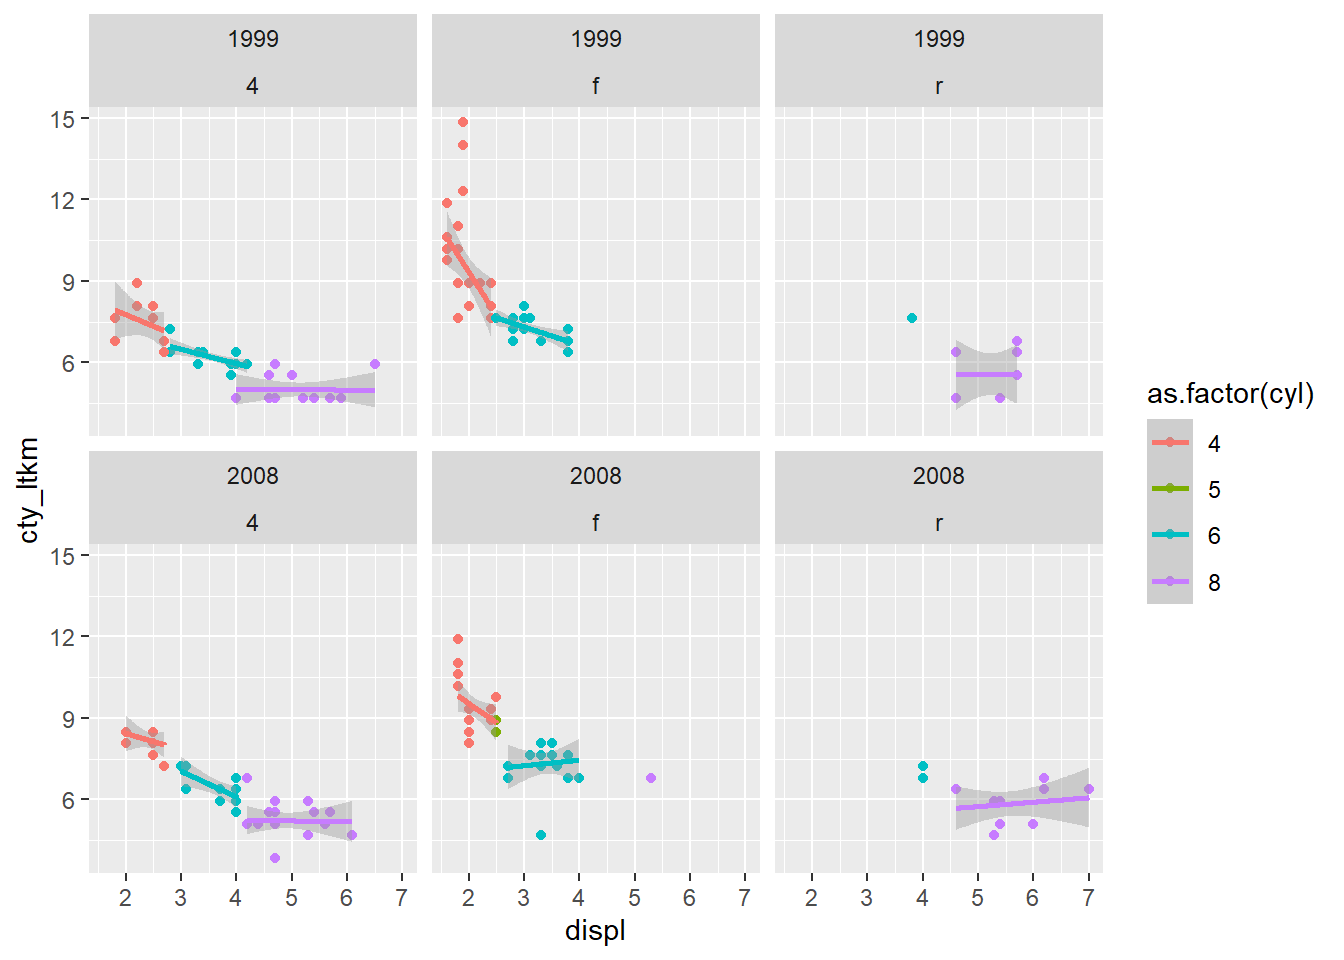
\includegraphics{ggplot2_files/figure-pdf/unnamed-chunk-1-8.pdf}

}

\end{figure}

\begin{Shaded}
\begin{Highlighting}[]
\NormalTok{p3 }\SpecialCharTok{+} \FunctionTok{facet\_grid}\NormalTok{(drv }\SpecialCharTok{\textasciitilde{}}\NormalTok{ year) }\CommentTok{\# eksen aralıkları sabit}
\end{Highlighting}
\end{Shaded}

\begin{verbatim}
`geom_smooth()` using formula = 'y ~ x'
\end{verbatim}

\begin{figure}[H]

{\centering 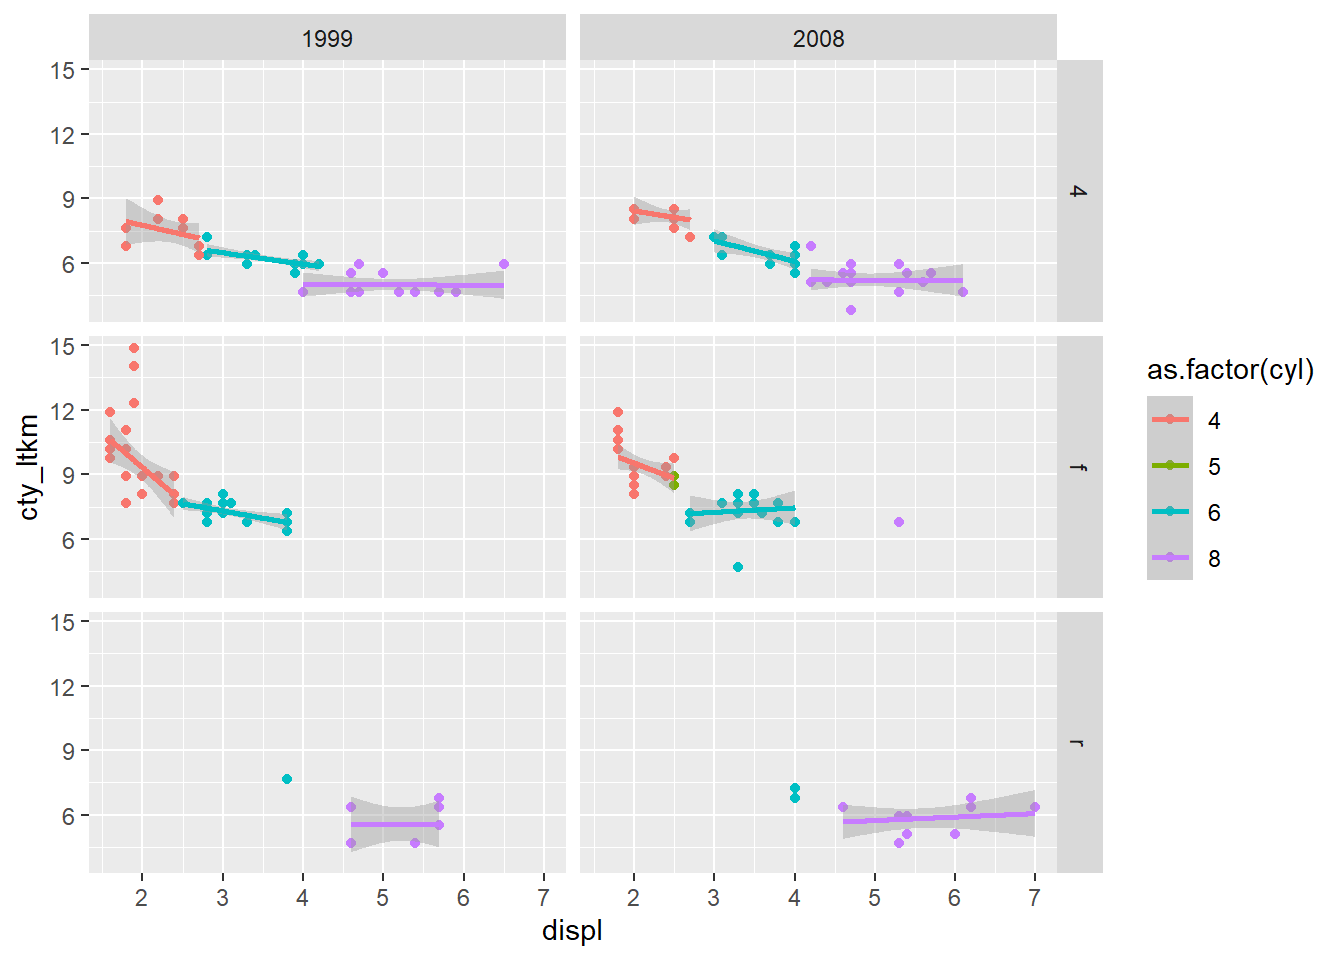
\includegraphics{ggplot2_files/figure-pdf/unnamed-chunk-1-9.pdf}

}

\end{figure}

\begin{Shaded}
\begin{Highlighting}[]
\NormalTok{p3 }\SpecialCharTok{+} \FunctionTok{facet\_grid}\NormalTok{(drv }\SpecialCharTok{\textasciitilde{}}\NormalTok{ year,}\AttributeTok{scales =} \StringTok{"free"}\NormalTok{) }\CommentTok{\# eksen aralıkları değişken}
\end{Highlighting}
\end{Shaded}

\begin{verbatim}
`geom_smooth()` using formula = 'y ~ x'
\end{verbatim}

\begin{figure}[H]

{\centering 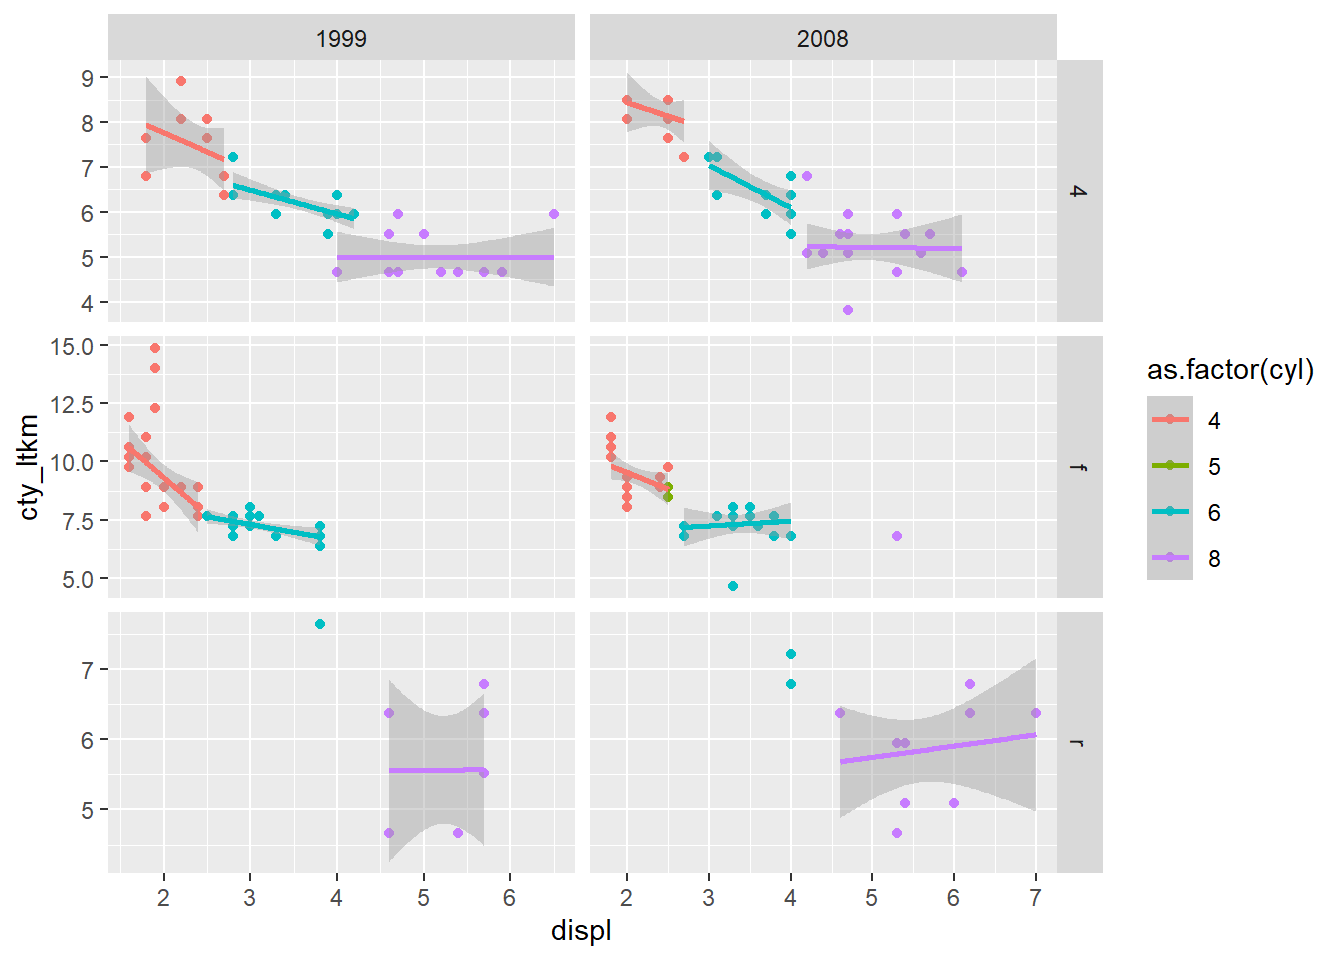
\includegraphics{ggplot2_files/figure-pdf/unnamed-chunk-1-10.pdf}

}

\end{figure}

\hypertarget{zaman-serisi-grafikleri}{%
\section*{Zaman Serisi Grafikleri}\label{zaman-serisi-grafikleri}}
\addcontentsline{toc}{section}{Zaman Serisi Grafikleri}

\markright{Zaman Serisi Grafikleri}

Zaman serisi grafikleri, zamanla değişen verileri görsel olarak temsil
etmek için kullanılan grafiklerdir. Bu tür grafikler, belirli bir süre
boyunca gözlemlenen verileri analiz etmek, eğilimleri belirlemek,
dönemsel desenleri tanımak ve istatistiksel analizler yapmak için yaygın
olarak kullanılır. Zaman serisi verileri genellikle sabit aralıklarla
veya farklı zaman dilimlerinde toplanır. En yaygın olan türü çizgi
grafikleri olmakla birlikte sütun ve alan grafikleri de zaman
serilerinin görselleştirilmesinde kullanılabilmektedir.

Örnekler ggplot2 paketi ile birlikte gelen
\href{https://ggplot2.tidyverse.org/reference/economics.html}{\textbf{\texttt{economics}}}
veri seti ile yapılacaktır.

\begin{Shaded}
\begin{Highlighting}[]
\NormalTok{economics}
\end{Highlighting}
\end{Shaded}

\begin{verbatim}
# A tibble: 574 x 6
   date         pce    pop psavert uempmed unemploy
   <date>     <dbl>  <dbl>   <dbl>   <dbl>    <dbl>
 1 1967-07-01  507. 198712    12.6     4.5     2944
 2 1967-08-01  510. 198911    12.6     4.7     2945
 3 1967-09-01  516. 199113    11.9     4.6     2958
 4 1967-10-01  512. 199311    12.9     4.9     3143
 5 1967-11-01  517. 199498    12.8     4.7     3066
 6 1967-12-01  525. 199657    11.8     4.8     3018
 7 1968-01-01  531. 199808    11.7     5.1     2878
 8 1968-02-01  534. 199920    12.3     4.5     3001
 9 1968-03-01  544. 200056    11.7     4.1     2877
10 1968-04-01  544  200208    12.3     4.6     2709
# i 564 more rows
\end{verbatim}

\begin{Shaded}
\begin{Highlighting}[]
\FunctionTok{summary}\NormalTok{(economics)}
\end{Highlighting}
\end{Shaded}

\begin{verbatim}
      date                 pce               pop            psavert      
 Min.   :1967-07-01   Min.   :  506.7   Min.   :198712   Min.   : 2.200  
 1st Qu.:1979-06-08   1st Qu.: 1578.3   1st Qu.:224896   1st Qu.: 6.400  
 Median :1991-05-16   Median : 3936.8   Median :253060   Median : 8.400  
 Mean   :1991-05-17   Mean   : 4820.1   Mean   :257160   Mean   : 8.567  
 3rd Qu.:2003-04-23   3rd Qu.: 7626.3   3rd Qu.:290291   3rd Qu.:11.100  
 Max.   :2015-04-01   Max.   :12193.8   Max.   :320402   Max.   :17.300  
    uempmed          unemploy    
 Min.   : 4.000   Min.   : 2685  
 1st Qu.: 6.000   1st Qu.: 6284  
 Median : 7.500   Median : 7494  
 Mean   : 8.609   Mean   : 7771  
 3rd Qu.: 9.100   3rd Qu.: 8686  
 Max.   :25.200   Max.   :15352  
\end{verbatim}

\begin{Shaded}
\begin{Highlighting}[]
\NormalTok{p4 }\OtherTok{\textless{}{-}}\NormalTok{ economics }\SpecialCharTok{\%\textgreater{}\%} 
  \FunctionTok{ggplot}\NormalTok{(}\FunctionTok{aes}\NormalTok{(}\AttributeTok{x=}\NormalTok{date,}\AttributeTok{y=}\NormalTok{pce)) }\SpecialCharTok{+}
  \FunctionTok{geom\_line}\NormalTok{(}\AttributeTok{color=}\StringTok{"blue"}\NormalTok{) }\SpecialCharTok{+}
  \FunctionTok{theme\_minimal}\NormalTok{() }\SpecialCharTok{+}
  \FunctionTok{labs}\NormalTok{(}\AttributeTok{x =} \StringTok{""}\NormalTok{,}
       \AttributeTok{y =} \StringTok{"Personal Consumption Expenditures"}\NormalTok{,}
       \AttributeTok{title =} \StringTok{"Personal Consumption Expenditures Time Series"}\NormalTok{,}
       \AttributeTok{caption =} \StringTok{"Economics Data"}\NormalTok{,}
       \AttributeTok{subtitle =} \StringTok{"Economics Data (1967{-}2015)"}\NormalTok{)}
\NormalTok{p4}
\end{Highlighting}
\end{Shaded}

\begin{figure}[H]

{\centering 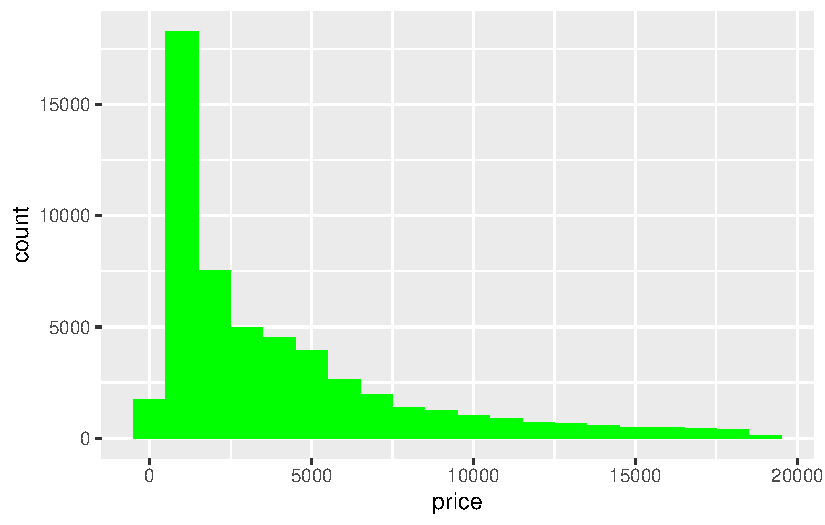
\includegraphics{ggplot2_files/figure-pdf/unnamed-chunk-2-1.pdf}

}

\end{figure}

\begin{Shaded}
\begin{Highlighting}[]
\CommentTok{\# zaman eksenini ayarlama}
\NormalTok{p4 }\SpecialCharTok{+} 
  \FunctionTok{scale\_x\_date}\NormalTok{(}\AttributeTok{date\_breaks =} \StringTok{"1 year"}\NormalTok{, }\AttributeTok{date\_labels =} \StringTok{"\%Y"}\NormalTok{) }\SpecialCharTok{+}
  \FunctionTok{theme}\NormalTok{(}\AttributeTok{axis.text.x =} \FunctionTok{element\_text}\NormalTok{(}\AttributeTok{angle =} \DecValTok{45}\NormalTok{), }\AttributeTok{legend.position =} \StringTok{"top"}\NormalTok{)}
\end{Highlighting}
\end{Shaded}

\begin{figure}[H]

{\centering \includegraphics{ggplot2_files/figure-pdf/unnamed-chunk-2-2.pdf}

}

\end{figure}

\begin{Shaded}
\begin{Highlighting}[]
\NormalTok{p4 }\SpecialCharTok{+} 
  \FunctionTok{scale\_x\_date}\NormalTok{(}\AttributeTok{date\_breaks =} \StringTok{"2 year"}\NormalTok{, }\AttributeTok{date\_labels =} \StringTok{"\%Y"}\NormalTok{,}\AttributeTok{expand =} \FunctionTok{c}\NormalTok{(}\DecValTok{0}\NormalTok{,}\DecValTok{0}\NormalTok{)) }\SpecialCharTok{+}
  \FunctionTok{theme}\NormalTok{(}\AttributeTok{axis.text.x =} \FunctionTok{element\_text}\NormalTok{(}\AttributeTok{angle =} \DecValTok{45}\NormalTok{), }\AttributeTok{legend.position =} \StringTok{"top"}\NormalTok{)}
\end{Highlighting}
\end{Shaded}

\begin{figure}[H]

{\centering \includegraphics{ggplot2_files/figure-pdf/unnamed-chunk-2-3.pdf}

}

\end{figure}

\begin{Shaded}
\begin{Highlighting}[]
\CommentTok{\# çizgi türü değiştirilebilir}
\NormalTok{economics }\SpecialCharTok{\%\textgreater{}\%} 
  \FunctionTok{ggplot}\NormalTok{(}\FunctionTok{aes}\NormalTok{(}\AttributeTok{x=}\NormalTok{date,}\AttributeTok{y=}\NormalTok{pce)) }\SpecialCharTok{+}
  \FunctionTok{geom\_line}\NormalTok{(}\AttributeTok{linetype =} \StringTok{"dashed"}\NormalTok{, }\AttributeTok{size =} \DecValTok{1}\NormalTok{, }\AttributeTok{colour =} \StringTok{"blue"}\NormalTok{)}
\end{Highlighting}
\end{Shaded}

\begin{verbatim}
Warning: Using `size` aesthetic for lines was deprecated in ggplot2 3.4.0.
i Please use `linewidth` instead.
\end{verbatim}

\begin{figure}[H]

{\centering \includegraphics{ggplot2_files/figure-pdf/unnamed-chunk-2-4.pdf}

}

\end{figure}

\begin{Shaded}
\begin{Highlighting}[]
\NormalTok{economics }\SpecialCharTok{\%\textgreater{}\%} 
  \FunctionTok{ggplot}\NormalTok{(}\FunctionTok{aes}\NormalTok{(}\AttributeTok{x=}\NormalTok{date,}\AttributeTok{y=}\NormalTok{pce)) }\SpecialCharTok{+}
  \FunctionTok{geom\_line}\NormalTok{(}\AttributeTok{linetype =} \StringTok{"dotted"}\NormalTok{, }\AttributeTok{size =} \DecValTok{2}\NormalTok{, }\AttributeTok{colour =} \StringTok{"blue"}\NormalTok{)}
\end{Highlighting}
\end{Shaded}

\begin{figure}[H]

{\centering \includegraphics{ggplot2_files/figure-pdf/unnamed-chunk-2-5.pdf}

}

\end{figure}

\begin{Shaded}
\begin{Highlighting}[]
\CommentTok{\# zaman grafiğine noktalar ekleme}
\NormalTok{economics }\SpecialCharTok{\%\textgreater{}\%} 
  \FunctionTok{filter}\NormalTok{(lubridate}\SpecialCharTok{::}\FunctionTok{year}\NormalTok{(date) }\SpecialCharTok{\textgreater{}=} \DecValTok{2010}\NormalTok{) }\SpecialCharTok{\%\textgreater{}\%} 
  \FunctionTok{ggplot}\NormalTok{(}\FunctionTok{aes}\NormalTok{(}\AttributeTok{x=}\NormalTok{date,}\AttributeTok{y=}\NormalTok{pce)) }\SpecialCharTok{+}
  \FunctionTok{geom\_line}\NormalTok{()}\SpecialCharTok{+}
  \FunctionTok{geom\_point}\NormalTok{(}\AttributeTok{size =} \DecValTok{3}\NormalTok{, }\AttributeTok{shape=} \DecValTok{7}\NormalTok{, }\AttributeTok{colour =} \StringTok{"red"}\NormalTok{)}
\end{Highlighting}
\end{Shaded}

\begin{figure}[H]

{\centering \includegraphics{ggplot2_files/figure-pdf/unnamed-chunk-2-6.pdf}

}

\end{figure}

\begin{Shaded}
\begin{Highlighting}[]
\CommentTok{\# gölgeli zaman grafiği}
\NormalTok{economics }\SpecialCharTok{\%\textgreater{}\%} 
  \FunctionTok{ggplot}\NormalTok{(}\FunctionTok{aes}\NormalTok{(}\AttributeTok{x=}\NormalTok{date,}\AttributeTok{y=}\NormalTok{pce)) }\SpecialCharTok{+}
  \FunctionTok{geom\_area}\NormalTok{(}\AttributeTok{color=}\StringTok{"blue"}\NormalTok{,}\AttributeTok{fill=}\StringTok{"red"}\NormalTok{,}\AttributeTok{alpha=}\FloatTok{0.6}\NormalTok{) }\SpecialCharTok{+}
  \CommentTok{\# y ekseni aralıklarını ayarlama}
  \FunctionTok{scale\_y\_continuous}\NormalTok{(}\AttributeTok{breaks =} \FunctionTok{seq}\NormalTok{(}\DecValTok{0}\NormalTok{, }\FunctionTok{max}\NormalTok{(economics}\SpecialCharTok{$}\NormalTok{pce), }\AttributeTok{by =} \DecValTok{1000}\NormalTok{))}
\end{Highlighting}
\end{Shaded}

\begin{figure}[H]

{\centering \includegraphics{ggplot2_files/figure-pdf/unnamed-chunk-2-7.pdf}

}

\end{figure}

\begin{Shaded}
\begin{Highlighting}[]
\NormalTok{economics }\SpecialCharTok{\%\textgreater{}\%} 
  \FunctionTok{ggplot}\NormalTok{(}\FunctionTok{aes}\NormalTok{(}\AttributeTok{x=}\NormalTok{date,}\AttributeTok{y=}\NormalTok{uempmed )) }\SpecialCharTok{+}
  \FunctionTok{geom\_area}\NormalTok{(}\AttributeTok{color=}\StringTok{"blue"}\NormalTok{,}\AttributeTok{fill=}\StringTok{"red"}\NormalTok{,}\AttributeTok{alpha=}\FloatTok{0.5}\NormalTok{) }\SpecialCharTok{+}
  \FunctionTok{theme\_light}\NormalTok{()}
\end{Highlighting}
\end{Shaded}

\begin{figure}[H]

{\centering \includegraphics{ggplot2_files/figure-pdf/unnamed-chunk-2-8.pdf}

}

\end{figure}

\begin{Shaded}
\begin{Highlighting}[]
\CommentTok{\# çoklu zaman serisi grafiği}
\NormalTok{economics\_long}
\end{Highlighting}
\end{Shaded}

\begin{verbatim}
# A tibble: 2,870 x 4
   date       variable value  value01
   <date>     <chr>    <dbl>    <dbl>
 1 1967-07-01 pce       507. 0       
 2 1967-08-01 pce       510. 0.000265
 3 1967-09-01 pce       516. 0.000762
 4 1967-10-01 pce       512. 0.000471
 5 1967-11-01 pce       517. 0.000916
 6 1967-12-01 pce       525. 0.00157 
 7 1968-01-01 pce       531. 0.00207 
 8 1968-02-01 pce       534. 0.00230 
 9 1968-03-01 pce       544. 0.00322 
10 1968-04-01 pce       544  0.00319 
# i 2,860 more rows
\end{verbatim}

\begin{Shaded}
\begin{Highlighting}[]
\CommentTok{\# serilerin ölçekleri farklı }
\NormalTok{economics\_long }\SpecialCharTok{\%\textgreater{}\%} 
  \FunctionTok{ggplot}\NormalTok{(}\FunctionTok{aes}\NormalTok{(}\AttributeTok{x=}\NormalTok{date,}\AttributeTok{y=}\NormalTok{value,}\AttributeTok{color=}\NormalTok{variable))}\SpecialCharTok{+}
  \FunctionTok{geom\_line}\NormalTok{()}
\end{Highlighting}
\end{Shaded}

\begin{figure}[H]

{\centering \includegraphics{ggplot2_files/figure-pdf/unnamed-chunk-2-9.pdf}

}

\end{figure}

\begin{Shaded}
\begin{Highlighting}[]
\NormalTok{economics\_long }\SpecialCharTok{\%\textgreater{}\%} 
  \FunctionTok{ggplot}\NormalTok{(}\FunctionTok{aes}\NormalTok{(}\AttributeTok{x=}\NormalTok{date,}\AttributeTok{y=}\NormalTok{value))}\SpecialCharTok{+}
  \FunctionTok{geom\_line}\NormalTok{() }\SpecialCharTok{+}
  \FunctionTok{facet\_wrap}\NormalTok{(}\SpecialCharTok{\textasciitilde{}}\NormalTok{variable,}\AttributeTok{scales =} \StringTok{"free\_y"}\NormalTok{)}
\end{Highlighting}
\end{Shaded}

\begin{figure}[H]

{\centering \includegraphics{ggplot2_files/figure-pdf/unnamed-chunk-2-10.pdf}

}

\end{figure}

\begin{Shaded}
\begin{Highlighting}[]
\NormalTok{economics\_long }\SpecialCharTok{\%\textgreater{}\%} 
  \FunctionTok{ggplot}\NormalTok{(}\FunctionTok{aes}\NormalTok{(}\AttributeTok{x=}\NormalTok{date,}\AttributeTok{y=}\NormalTok{value))}\SpecialCharTok{+}
  \FunctionTok{geom\_line}\NormalTok{() }\SpecialCharTok{+}
  \FunctionTok{facet\_wrap}\NormalTok{(}\SpecialCharTok{\textasciitilde{}}\NormalTok{variable,}\AttributeTok{scales =} \StringTok{"free\_y"}\NormalTok{)}\SpecialCharTok{+}
  \FunctionTok{scale\_y\_log10}\NormalTok{() }\CommentTok{\# y eksenlerinin logatirması alınır}
\end{Highlighting}
\end{Shaded}

\begin{figure}[H]

{\centering \includegraphics{ggplot2_files/figure-pdf/unnamed-chunk-2-11.pdf}

}

\end{figure}

\hypertarget{suxfctun-grafikleri}{%
\section*{Sütun Grafikleri}\label{suxfctun-grafikleri}}
\addcontentsline{toc}{section}{Sütun Grafikleri}

\markright{Sütun Grafikleri}

Sütun grafikleri, verileri kategorik veya gruplara göre temsil etmek
için kullanılan bir grafik türüdür. Bu grafik türü, farklı kategorilerin
veya grupların sayısal değerlerini karşılaştırmak veya görselleştirmek
için kullanılır. Sütun grafikleri dikey çubuklardan oluşur ve her çubuk,
bir kategori veya grup için bir değeri temsil eder. Sütun grafiklerinin
temel bileşenleri şunlardır:

\begin{enumerate}
\def\labelenumi{\arabic{enumi}.}
\item
  \textbf{Yatay Eksen (X-Eksen):} Bu eksende kategoriler veya gruplar
  yer alır. Örneğin, bir yıl boyunca aylar, ürün kategorileri, bölgeler
  veya şirket departmanları gibi farklı kategoriler olabilir.
\item
  \textbf{Dikey Eksen (Y-Eksen):} Bu eksende sayısal değerler yer alır
  ve sütunların yükseklikleri bu değerleri temsil eder. Değerler
  genellikle sayısal verilerdir ve karşılaştırılabilir bir ölçü birimi
  içinde bulunurlar.
\item
  \textbf{Sütunlar:} Sütunlar, her bir kategori veya grup için bir
  değeri temsil eder. Sütunların yükseklikleri, karşılaştırılan
  değerlerin büyüklüğünü veya ilişkilerini gösterir.
\end{enumerate}

Sütun grafikleri, aşağıdaki amaçlar için kullanılır:

\begin{itemize}
\item
  Karşılaştırmalar: Farklı kategorilerin veya grupların değerlerini
  karşılaştırmak için kullanılır. Örneğin, farklı ülkelerin gayri safi
  yurtiçi hasıla (GSYİH) değerlerini karşılaştırmak için sütun
  grafikleri kullanılabilir.
\item
  Zaman İçi Değişim: Zaman serisi verilerini temsil etmek için
  kullanılabilir. Her sütun, belirli bir zaman dilimindeki değerleri
  gösterebilir.
\item
  Kategorik Verilerin İncelenmesi: Ürün kategorileri, şirket
  departmanları veya müşteri segmentleri gibi kategorik verilerin
  analizi için kullanılabilir.
\end{itemize}

Sütun grafikleri, verileri görsel olarak anlamak ve veriler arasındaki
farkları veya eğilimleri vurgulamak için etkili bir araçtır. Aynı
zamanda verilerin daha kolay anlaşılmasına yardımcı olabilir ve karar
verme süreçlerine katkı sağlayabilir.

Örnekler ggplot2 paketi ile birlikte gelen
\href{https://ggplot2.tidyverse.org/reference/diamonds.html}{\textbf{\texttt{diamonds}}}
veri seti ile yapılacaktır.

\begin{Shaded}
\begin{Highlighting}[]
\NormalTok{diamonds}
\end{Highlighting}
\end{Shaded}

\begin{verbatim}
# A tibble: 53,940 x 10
   carat cut       color clarity depth table price     x     y     z
   <dbl> <ord>     <ord> <ord>   <dbl> <dbl> <int> <dbl> <dbl> <dbl>
 1  0.23 Ideal     E     SI2      61.5    55   326  3.95  3.98  2.43
 2  0.21 Premium   E     SI1      59.8    61   326  3.89  3.84  2.31
 3  0.23 Good      E     VS1      56.9    65   327  4.05  4.07  2.31
 4  0.29 Premium   I     VS2      62.4    58   334  4.2   4.23  2.63
 5  0.31 Good      J     SI2      63.3    58   335  4.34  4.35  2.75
 6  0.24 Very Good J     VVS2     62.8    57   336  3.94  3.96  2.48
 7  0.24 Very Good I     VVS1     62.3    57   336  3.95  3.98  2.47
 8  0.26 Very Good H     SI1      61.9    55   337  4.07  4.11  2.53
 9  0.22 Fair      E     VS2      65.1    61   337  3.87  3.78  2.49
10  0.23 Very Good H     VS1      59.4    61   338  4     4.05  2.39
# i 53,930 more rows
\end{verbatim}

\begin{Shaded}
\begin{Highlighting}[]
\FunctionTok{glimpse}\NormalTok{(diamonds)}
\end{Highlighting}
\end{Shaded}

\begin{verbatim}
Rows: 53,940
Columns: 10
$ carat   <dbl> 0.23, 0.21, 0.23, 0.29, 0.31, 0.24, 0.24, 0.26, 0.22, 0.23, 0.~
$ cut     <ord> Ideal, Premium, Good, Premium, Good, Very Good, Very Good, Ver~
$ color   <ord> E, E, E, I, J, J, I, H, E, H, J, J, F, J, E, E, I, J, J, J, I,~
$ clarity <ord> SI2, SI1, VS1, VS2, SI2, VVS2, VVS1, SI1, VS2, VS1, SI1, VS1, ~
$ depth   <dbl> 61.5, 59.8, 56.9, 62.4, 63.3, 62.8, 62.3, 61.9, 65.1, 59.4, 64~
$ table   <dbl> 55, 61, 65, 58, 58, 57, 57, 55, 61, 61, 55, 56, 61, 54, 62, 58~
$ price   <int> 326, 326, 327, 334, 335, 336, 336, 337, 337, 338, 339, 340, 34~
$ x       <dbl> 3.95, 3.89, 4.05, 4.20, 4.34, 3.94, 3.95, 4.07, 3.87, 4.00, 4.~
$ y       <dbl> 3.98, 3.84, 4.07, 4.23, 4.35, 3.96, 3.98, 4.11, 3.78, 4.05, 4.~
$ z       <dbl> 2.43, 2.31, 2.31, 2.63, 2.75, 2.48, 2.47, 2.53, 2.49, 2.39, 2.~
\end{verbatim}

\begin{Shaded}
\begin{Highlighting}[]
\FunctionTok{summary}\NormalTok{(diamonds)}
\end{Highlighting}
\end{Shaded}

\begin{verbatim}
     carat               cut        color        clarity          depth      
 Min.   :0.2000   Fair     : 1610   D: 6775   SI1    :13065   Min.   :43.00  
 1st Qu.:0.4000   Good     : 4906   E: 9797   VS2    :12258   1st Qu.:61.00  
 Median :0.7000   Very Good:12082   F: 9542   SI2    : 9194   Median :61.80  
 Mean   :0.7979   Premium  :13791   G:11292   VS1    : 8171   Mean   :61.75  
 3rd Qu.:1.0400   Ideal    :21551   H: 8304   VVS2   : 5066   3rd Qu.:62.50  
 Max.   :5.0100                     I: 5422   VVS1   : 3655   Max.   :79.00  
                                    J: 2808   (Other): 2531                  
     table           price             x                y         
 Min.   :43.00   Min.   :  326   Min.   : 0.000   Min.   : 0.000  
 1st Qu.:56.00   1st Qu.:  950   1st Qu.: 4.710   1st Qu.: 4.720  
 Median :57.00   Median : 2401   Median : 5.700   Median : 5.710  
 Mean   :57.46   Mean   : 3933   Mean   : 5.731   Mean   : 5.735  
 3rd Qu.:59.00   3rd Qu.: 5324   3rd Qu.: 6.540   3rd Qu.: 6.540  
 Max.   :95.00   Max.   :18823   Max.   :10.740   Max.   :58.900  
                                                                  
       z         
 Min.   : 0.000  
 1st Qu.: 2.910  
 Median : 3.530  
 Mean   : 3.539  
 3rd Qu.: 4.040  
 Max.   :31.800  
                 
\end{verbatim}

\begin{Shaded}
\begin{Highlighting}[]
\CommentTok{\# sıklık durumunu görselleştirme}
\FunctionTok{ggplot}\NormalTok{(diamonds, }\FunctionTok{aes}\NormalTok{(cut)) }\SpecialCharTok{+}
  \FunctionTok{geom\_bar}\NormalTok{()}
\end{Highlighting}
\end{Shaded}

\begin{figure}[H]

{\centering \includegraphics{ggplot2_files/figure-pdf/unnamed-chunk-3-1.pdf}

}

\end{figure}

\begin{Shaded}
\begin{Highlighting}[]
\FunctionTok{ggplot}\NormalTok{(diamonds, }\FunctionTok{aes}\NormalTok{(cut, }\AttributeTok{fill =}\NormalTok{ color)) }\SpecialCharTok{+}
  \FunctionTok{geom\_bar}\NormalTok{(}\AttributeTok{position =} \FunctionTok{position\_dodge}\NormalTok{()) }\SpecialCharTok{+} 
  \FunctionTok{xlab}\NormalTok{(}\StringTok{"Pirlanta kaliteleri"}\NormalTok{) }\SpecialCharTok{+} 
  \FunctionTok{ylab}\NormalTok{(}\StringTok{"Gozlenme Sikliklari"}\NormalTok{)}
\end{Highlighting}
\end{Shaded}

\begin{figure}[H]

{\centering \includegraphics{ggplot2_files/figure-pdf/unnamed-chunk-3-2.pdf}

}

\end{figure}

\begin{Shaded}
\begin{Highlighting}[]
\FunctionTok{ggplot}\NormalTok{(diamonds, }\FunctionTok{aes}\NormalTok{(}\AttributeTok{x=}\NormalTok{cut, }\AttributeTok{y=}\NormalTok{carat,}\AttributeTok{fill =}\NormalTok{ color)) }\SpecialCharTok{+}
  \FunctionTok{geom\_bar}\NormalTok{(}\AttributeTok{stat =} \StringTok{"identity"}\NormalTok{) }
\end{Highlighting}
\end{Shaded}

\begin{figure}[H]

{\centering \includegraphics{ggplot2_files/figure-pdf/unnamed-chunk-3-3.pdf}

}

\end{figure}

\begin{Shaded}
\begin{Highlighting}[]
\FunctionTok{ggplot}\NormalTok{(diamonds, }\FunctionTok{aes}\NormalTok{(}\AttributeTok{x=}\NormalTok{cut, }\AttributeTok{y=}\NormalTok{carat,}\AttributeTok{fill =}\NormalTok{ color)) }\SpecialCharTok{+}
  \CommentTok{\# fill ile oransal olarak gösterim yapılır}
  \FunctionTok{geom\_bar}\NormalTok{(}\AttributeTok{stat =} \StringTok{"identity"}\NormalTok{,}\AttributeTok{position =} \StringTok{"fill"}\NormalTok{) }
\end{Highlighting}
\end{Shaded}

\begin{figure}[H]

{\centering \includegraphics{ggplot2_files/figure-pdf/unnamed-chunk-3-4.pdf}

}

\end{figure}

\begin{Shaded}
\begin{Highlighting}[]
\FunctionTok{ggplot}\NormalTok{(diamonds, }\FunctionTok{aes}\NormalTok{(}\AttributeTok{x=}\NormalTok{cut,}\AttributeTok{y=}\NormalTok{carat, }\AttributeTok{fill =}\NormalTok{ color)) }\SpecialCharTok{+}
  \FunctionTok{geom\_col}\NormalTok{() }\CommentTok{\# y ekseni toplanarak yığılmış}
\end{Highlighting}
\end{Shaded}

\begin{figure}[H]

{\centering \includegraphics{ggplot2_files/figure-pdf/unnamed-chunk-3-5.pdf}

}

\end{figure}

\begin{Shaded}
\begin{Highlighting}[]
\FunctionTok{ggplot}\NormalTok{(diamonds, }\FunctionTok{aes}\NormalTok{(}\AttributeTok{x=}\NormalTok{cut,}\AttributeTok{y=}\NormalTok{carat,, }\AttributeTok{fill =}\NormalTok{ color)) }\SpecialCharTok{+}
  \FunctionTok{geom\_col}\NormalTok{(}\AttributeTok{position =} \StringTok{"dodge"}\NormalTok{) }\CommentTok{\# y ekseni değerleri}
\end{Highlighting}
\end{Shaded}

\begin{figure}[H]

{\centering \includegraphics{ggplot2_files/figure-pdf/unnamed-chunk-3-6.pdf}

}

\end{figure}

\begin{Shaded}
\begin{Highlighting}[]
\FunctionTok{ggplot}\NormalTok{(diamonds, }\FunctionTok{aes}\NormalTok{(}\AttributeTok{x=}\NormalTok{cut,}\AttributeTok{y=}\NormalTok{carat, }\AttributeTok{fill =}\NormalTok{ color)) }\SpecialCharTok{+}
  \FunctionTok{geom\_col}\NormalTok{(}\AttributeTok{position =} \StringTok{"stack"}\NormalTok{)}
\end{Highlighting}
\end{Shaded}

\begin{figure}[H]

{\centering \includegraphics{ggplot2_files/figure-pdf/unnamed-chunk-3-7.pdf}

}

\end{figure}

\hypertarget{daux11fux131lux131m-grafikleri}{%
\section*{Dağılım Grafikleri}\label{daux11fux131lux131m-grafikleri}}
\addcontentsline{toc}{section}{Dağılım Grafikleri}

\markright{Dağılım Grafikleri}

Dağılım grafikleri, veri setinin dağılımını görsel olarak temsil etmek
için kullanılan grafik türleridir. Bu grafikler, veri noktalarının,
değerlerinin veya gözlemlerinin nasıl dağıldığını incelemek ve veri
setindeki desenleri, eğilimleri ve aykırı değerleri anlamak için
kullanılır. En yaygın olanı histogram grafikleridir.

Histogram, veri setinin sayısal dağılımını gösteren bir grafiktir. Veri
aralığı belli bir aralığa bölen çubuklardan oluşur ve her çubuk, bu
aralıktaki veri noktalarının sayısını temsil eder. Histogramlar
genellikle sürekli verilerin dağılımını göstermek için kullanılır.

Bunun dışında boxplot (kutu) grafikleri de dağılımı görselleştirmek için
kullanılmaktadır. Boxplot, veri setinin beş özet istatistiği (minimum,
ilk çeyrek, medyan, üçüncü çeyrek, maksimum) kullanarak veri dağılımını
temsil eder. Bu grafik, aykırı değerleri tanımlamak ve merkezi eğilim
ile dağılımın yayılmasını görsel olarak incelemek için kullanılır.

\begin{Shaded}
\begin{Highlighting}[]
\FunctionTok{ggplot}\NormalTok{(diamonds, }\FunctionTok{aes}\NormalTok{(price)) }\SpecialCharTok{+}
  \FunctionTok{geom\_histogram}\NormalTok{()}
\end{Highlighting}
\end{Shaded}

\begin{verbatim}
`stat_bin()` using `bins = 30`. Pick better value with `binwidth`.
\end{verbatim}

\begin{figure}[H]

{\centering \includegraphics{ggplot2_files/figure-pdf/unnamed-chunk-4-1.pdf}

}

\end{figure}

\begin{Shaded}
\begin{Highlighting}[]
\FunctionTok{ggplot}\NormalTok{(diamonds, }\FunctionTok{aes}\NormalTok{(price)) }\SpecialCharTok{+}
  \FunctionTok{geom\_histogram}\NormalTok{(}\AttributeTok{binwidth =} \DecValTok{1000}\NormalTok{,}\AttributeTok{fill =} \StringTok{"green"}\NormalTok{)}
\end{Highlighting}
\end{Shaded}

\begin{figure}[H]

{\centering \includegraphics{ggplot2_files/figure-pdf/unnamed-chunk-4-2.pdf}

}

\end{figure}

\begin{Shaded}
\begin{Highlighting}[]
\FunctionTok{ggplot}\NormalTok{(diamonds, }\FunctionTok{aes}\NormalTok{(price)) }\SpecialCharTok{+}
  \FunctionTok{geom\_density}\NormalTok{()}
\end{Highlighting}
\end{Shaded}

\begin{figure}[H]

{\centering \includegraphics{ggplot2_files/figure-pdf/unnamed-chunk-4-3.pdf}

}

\end{figure}

\begin{Shaded}
\begin{Highlighting}[]
\FunctionTok{ggplot}\NormalTok{(diamonds, }\FunctionTok{aes}\NormalTok{(price)) }\SpecialCharTok{+}
  \FunctionTok{geom\_density}\NormalTok{(}\AttributeTok{alpha =}\NormalTok{ .}\DecValTok{3}\NormalTok{, }\AttributeTok{fill =} \StringTok{"blue"}\NormalTok{)}
\end{Highlighting}
\end{Shaded}

\begin{figure}[H]

{\centering \includegraphics{ggplot2_files/figure-pdf/unnamed-chunk-4-4.pdf}

}

\end{figure}

\begin{Shaded}
\begin{Highlighting}[]
\FunctionTok{ggplot}\NormalTok{(diamonds, }\FunctionTok{aes}\NormalTok{(price)) }\SpecialCharTok{+}
  \FunctionTok{geom\_histogram}\NormalTok{(}\FunctionTok{aes}\NormalTok{(}\AttributeTok{y =}\NormalTok{ ..density..),}\AttributeTok{fill =} \StringTok{"red"}\NormalTok{) }\SpecialCharTok{+}
  \FunctionTok{geom\_density}\NormalTok{(}\AttributeTok{size=}\DecValTok{1}\NormalTok{,}\AttributeTok{fill =} \StringTok{"blue"}\NormalTok{)}
\end{Highlighting}
\end{Shaded}

\begin{verbatim}
Warning: The dot-dot notation (`..density..`) was deprecated in ggplot2 3.4.0.
i Please use `after_stat(density)` instead.
\end{verbatim}

\begin{verbatim}
`stat_bin()` using `bins = 30`. Pick better value with `binwidth`.
\end{verbatim}

\begin{figure}[H]

{\centering \includegraphics{ggplot2_files/figure-pdf/unnamed-chunk-4-5.pdf}

}

\end{figure}

\begin{Shaded}
\begin{Highlighting}[]
\FunctionTok{ggplot}\NormalTok{(diamonds, }\FunctionTok{aes}\NormalTok{(price)) }\SpecialCharTok{+}
  \FunctionTok{geom\_histogram}\NormalTok{() }\SpecialCharTok{+} 
  \FunctionTok{facet\_wrap}\NormalTok{( }\SpecialCharTok{\textasciitilde{}}\NormalTok{ cut ,}\AttributeTok{scales =} \StringTok{"free"}\NormalTok{ )}
\end{Highlighting}
\end{Shaded}

\begin{verbatim}
`stat_bin()` using `bins = 30`. Pick better value with `binwidth`.
\end{verbatim}

\begin{figure}[H]

{\centering \includegraphics{ggplot2_files/figure-pdf/unnamed-chunk-4-6.pdf}

}

\end{figure}

\begin{Shaded}
\begin{Highlighting}[]
\FunctionTok{ggplot}\NormalTok{(diamonds, }\FunctionTok{aes}\NormalTok{(price)) }\SpecialCharTok{+}
  \FunctionTok{geom\_histogram}\NormalTok{() }\SpecialCharTok{+} 
  \FunctionTok{facet\_grid}\NormalTok{(cut }\SpecialCharTok{\textasciitilde{}}\NormalTok{ color,}\AttributeTok{scales =} \StringTok{"free"}\NormalTok{ )}
\end{Highlighting}
\end{Shaded}

\begin{verbatim}
`stat_bin()` using `bins = 30`. Pick better value with `binwidth`.
\end{verbatim}

\begin{figure}[H]

{\centering \includegraphics{ggplot2_files/figure-pdf/unnamed-chunk-4-7.pdf}

}

\end{figure}

\begin{Shaded}
\begin{Highlighting}[]
\FunctionTok{ggplot}\NormalTok{(diamonds, }\FunctionTok{aes}\NormalTok{(}\AttributeTok{x=}\NormalTok{price,}\AttributeTok{fill=}\NormalTok{cut)) }\SpecialCharTok{+}
  \FunctionTok{geom\_density}\NormalTok{(}\AttributeTok{alpha=}\NormalTok{.}\DecValTok{3}\NormalTok{)}
\end{Highlighting}
\end{Shaded}

\begin{figure}[H]

{\centering \includegraphics{ggplot2_files/figure-pdf/unnamed-chunk-4-8.pdf}

}

\end{figure}

\begin{Shaded}
\begin{Highlighting}[]
\CommentTok{\# boxplot}
\FunctionTok{ggplot}\NormalTok{(diamonds, }\FunctionTok{aes}\NormalTok{(}\AttributeTok{x=}\NormalTok{price)) }\SpecialCharTok{+}
  \FunctionTok{geom\_boxplot}\NormalTok{()}
\end{Highlighting}
\end{Shaded}

\begin{figure}[H]

{\centering \includegraphics{ggplot2_files/figure-pdf/unnamed-chunk-4-9.pdf}

}

\end{figure}

\begin{Shaded}
\begin{Highlighting}[]
\CommentTok{\# boxplot\textquotesingle{}a ortalama eklemek}
\FunctionTok{ggplot}\NormalTok{(diamonds, }\FunctionTok{aes}\NormalTok{(}\AttributeTok{x=}\NormalTok{cut,}\AttributeTok{y=}\NormalTok{price)) }\SpecialCharTok{+}
  \FunctionTok{geom\_boxplot}\NormalTok{(}\AttributeTok{color=}\StringTok{"blue"}\NormalTok{)}\SpecialCharTok{+}
  \FunctionTok{stat\_summary}\NormalTok{(}\AttributeTok{fun =} \StringTok{"mean"}\NormalTok{, }\AttributeTok{geom =} \StringTok{"point"}\NormalTok{, }\AttributeTok{shape =} \DecValTok{5}\NormalTok{, }\AttributeTok{size =} \DecValTok{3}\NormalTok{)}
\end{Highlighting}
\end{Shaded}

\begin{figure}[H]

{\centering \includegraphics{ggplot2_files/figure-pdf/unnamed-chunk-4-10.pdf}

}

\end{figure}

\hypertarget{grafiklerin-kaydedilmesi}{%
\section*{Grafiklerin Kaydedilmesi}\label{grafiklerin-kaydedilmesi}}
\addcontentsline{toc}{section}{Grafiklerin Kaydedilmesi}

\markright{Grafiklerin Kaydedilmesi}

Grafik oluşturulduktan sonra, grafik objesini bir değişkende
saklayabilirsiniz (aşağıdaki örnekte ``grafik'' adını kullandık). Grafik
objesini bir değişkende sakladıktan sonra, \textbf{\texttt{ggsave()}}
fonksiyonunu kullanarak grafik dosyasını kaydedebilirsiniz. Grafikleri
ayrıca RStudio penceresinin sağ alt kısmında yer alan \textbf{Plots}
sekmesindeki \textbf{\texttt{Export}} ile kayıt altına alabilirsiniz.

\begin{Shaded}
\begin{Highlighting}[]
\NormalTok{grafik }\OtherTok{\textless{}{-}}\NormalTok{ economics }\SpecialCharTok{\%\textgreater{}\%} 
  \FunctionTok{mutate}\NormalTok{(}\AttributeTok{uemploy\_mom=}\NormalTok{unemploy}\SpecialCharTok{/}\FunctionTok{lag}\NormalTok{(unemploy ) }\SpecialCharTok{*} \DecValTok{100} \SpecialCharTok{{-}} \DecValTok{100}\NormalTok{,}
         \AttributeTok{growth=}\FunctionTok{ifelse}\NormalTok{(uemploy\_mom}\SpecialCharTok{\textgreater{}}\DecValTok{0}\NormalTok{,}\StringTok{"pozitif"}\NormalTok{,}\StringTok{"negatif"}\NormalTok{)) }\SpecialCharTok{\%\textgreater{}\%} 
  \FunctionTok{na.omit}\NormalTok{() }\SpecialCharTok{\%\textgreater{}\%} 
  \FunctionTok{filter}\NormalTok{(lubridate}\SpecialCharTok{::}\FunctionTok{year}\NormalTok{(date)}\SpecialCharTok{\textgreater{}=}\DecValTok{2010}\NormalTok{) }\SpecialCharTok{\%\textgreater{}\%} 
  \FunctionTok{ggplot}\NormalTok{(}\FunctionTok{aes}\NormalTok{(}\AttributeTok{x=}\NormalTok{date,}\AttributeTok{y=}\NormalTok{uemploy\_mom,}\AttributeTok{fill=}\NormalTok{growth))}\SpecialCharTok{+}
  \FunctionTok{geom\_col}\NormalTok{() }\SpecialCharTok{+}
  \FunctionTok{theme}\NormalTok{(}\AttributeTok{legend.position =} \StringTok{"none"}\NormalTok{) }\SpecialCharTok{+}
  \FunctionTok{labs}\NormalTok{(}\AttributeTok{y=}\StringTok{"Aylık Değişim"}\NormalTok{,}
       \AttributeTok{title=}\StringTok{"Yıllara göre Aylık İstihdam Değişimi (2010{-}2015)"}\NormalTok{)}

\FunctionTok{ggsave}\NormalTok{(}\StringTok{"grafik1.png"}\NormalTok{, grafik, }\AttributeTok{width =} \DecValTok{20}\NormalTok{, }\AttributeTok{height =} \DecValTok{8}\NormalTok{, }\AttributeTok{units =} \StringTok{"cm"}\NormalTok{)}
\FunctionTok{ggsave}\NormalTok{(}\StringTok{"grafik1.png"}\NormalTok{, grafik,}\AttributeTok{width =} \DecValTok{20}\NormalTok{, }\AttributeTok{height =} \DecValTok{8}\NormalTok{, }\AttributeTok{unit =} \StringTok{"cm"}\NormalTok{, }\AttributeTok{dpi =} \DecValTok{300}\NormalTok{)}
\end{Highlighting}
\end{Shaded}

\bookmarksetup{startatroot}

\hypertarget{veri-uxf6n-iux15fleme}{%
\chapter*{Veri Ön İşleme}\label{veri-uxf6n-iux15fleme}}
\addcontentsline{toc}{chapter}{Veri Ön İşleme}

\markboth{Veri Ön İşleme}{Veri Ön İşleme}

Veri ön işleme; istatistiksel modeller kurulmadan önce veri seti
üzerinde yapılan bir takım düzeltme, eksik veriyi tamamlama, tekrarlanan
verileri kaldırma, dönüştürme, bütünleştirme, temizleme, normalleştirme,
boyut indirgeme vb. işlemlerdir. Bu aşamada ister istemez veri üzerinde
bilgi keşfi yapılmış olur. Veri önişleme istatistiksel bir modelleme
sürecinin büyük kısmını oluşturmaktadır. Kesin bir rakam olmamakla
birlikte modelleme sürecinin yarısından fazlasının bu aşamada
harcandığını ifade edebiliriz. Veri ön işleme temel anlamda 4 aşamadan
oluşmaktadır. Bunlar sırasıyla şu şekildedir:

\begin{enumerate}
\def\labelenumi{\arabic{enumi}.}
\item
  \textbf{Veri Temizleme :} Eksik verilerin tamamlanması, aykırı
  değerlerin teşhis edilmesi ve verilerdeki tutarsızlıkların giderilmesi
  gibi işlemler yapılmaktadır.
\item
  \textbf{Veri Birleştirme:} Farklı farklı veri tabanlarında bulunan
  veri setlerinin tek bir yerde toplanması aşamasının düzenli bir
  şekilde yürütülmesi sağlanır.
\item
  \textbf{Veri Dönüştürme :} Bu aşamada veriler, modelleme için uygun
  formlara dönüştürülürler. Veri dönüştürme; düzeltme, birleştirme,
  genelleştirme ve normalleştirme gibi değişik işlemlerden biri veya bir
  kaçını içerebilir. Veri normalleştirme , min-max dönüşümü, z
  standartlaştırması gibi yöntemler en sık kullanılan veri dönüştürme
  işlemlerinden bazılarıdır.
\item
  \textbf{Veri İndirgeme :} Daha küçük hacimli olarak veri kümesinin
  indirgenmiş bir örneğinin elde edilmesi amacıyla uygulanır. Bu sayede
  elde edilen indirgenmiş veri kümesine modelleme teknikleri uygulanarak
  daha etkin sonuçlar elde edilebilir. Veri Birleştirme (Data
  Aggregation), Boyut indirgeme (Dimension Reduction), Veri Sıkıştırma
  (Data Compression), Kesikli hale getirme (Discretization), Özellik
  Seçimi (Feature Selection) sık kullanılan veri indirgeme
  işlemlerindendir.
\end{enumerate}

Bu dokümanda eksik veriler (missing values), aykırı değerler (outliers)
ve veri normalleştirme işlemleri R uygulamları ile anlatılacaktır.

\hypertarget{eksik-veriler}{%
\section*{Eksik Veriler}\label{eksik-veriler}}
\addcontentsline{toc}{section}{Eksik Veriler}

\markright{Eksik Veriler}

Eksik veriler (kayıp gözlem), veri toplamada kaçınılmaz bir durumdur ve
üzerinde dikkatle durulmalıdır. Sistematik bir kayıp gözlem durumu yoksa
ortada ciddi bir sorun yoktur. Ama rastgele olmayan bir hata varsa tüm
kitleye dair yanlılık olacağı için bu durum göz ardı edilemez.

\begin{Shaded}
\begin{Highlighting}[]
\NormalTok{df }\OtherTok{\textless{}{-}} \FunctionTok{data.frame}\NormalTok{(}\AttributeTok{weight =} \FunctionTok{c}\NormalTok{(}\FunctionTok{rnorm}\NormalTok{(}\DecValTok{15}\NormalTok{, }\DecValTok{70}\NormalTok{, }\DecValTok{10}\NormalTok{), }\FunctionTok{rep}\NormalTok{(}\ConstantTok{NA}\NormalTok{, }\DecValTok{5}\NormalTok{)),}
                 \AttributeTok{height =} \FunctionTok{c}\NormalTok{(}\FunctionTok{rnorm}\NormalTok{(}\DecValTok{17}\NormalTok{, }\DecValTok{165}\NormalTok{, }\DecValTok{20}\NormalTok{), }\FunctionTok{rep}\NormalTok{(}\ConstantTok{NA}\NormalTok{, }\DecValTok{3}\NormalTok{)))}

\FunctionTok{set.seed}\NormalTok{(}\DecValTok{12345}\NormalTok{)}
\NormalTok{rows }\OtherTok{\textless{}{-}} \FunctionTok{sample}\NormalTok{(}\FunctionTok{nrow}\NormalTok{(df))}
\NormalTok{df2 }\OtherTok{\textless{}{-}}\NormalTok{ df[rows, ]}

\CommentTok{\# eksik verilerin sorgulanması}

\FunctionTok{is.na}\NormalTok{(df2) }\CommentTok{\# sorgulanma}
\end{Highlighting}
\end{Shaded}

\begin{verbatim}
   weight height
14  FALSE  FALSE
19   TRUE   TRUE
16   TRUE  FALSE
11  FALSE  FALSE
18   TRUE   TRUE
8   FALSE  FALSE
2   FALSE  FALSE
6   FALSE  FALSE
17   TRUE  FALSE
13  FALSE  FALSE
7   FALSE  FALSE
1   FALSE  FALSE
15  FALSE  FALSE
10  FALSE  FALSE
12  FALSE  FALSE
9   FALSE  FALSE
4   FALSE  FALSE
20   TRUE   TRUE
3   FALSE  FALSE
5   FALSE  FALSE
\end{verbatim}

\begin{Shaded}
\begin{Highlighting}[]
\FunctionTok{which}\NormalTok{(}\FunctionTok{is.na}\NormalTok{(df2)) }\CommentTok{\#konum}
\end{Highlighting}
\end{Shaded}

\begin{verbatim}
[1]  2  3  5  9 18 22 25 38
\end{verbatim}

\begin{Shaded}
\begin{Highlighting}[]
\FunctionTok{sum}\NormalTok{(}\FunctionTok{is.na}\NormalTok{(df2)) }\CommentTok{\# toplam eksik veri sayısı}
\end{Highlighting}
\end{Shaded}

\begin{verbatim}
[1] 8
\end{verbatim}

\begin{Shaded}
\begin{Highlighting}[]
\FunctionTok{colSums}\NormalTok{(}\FunctionTok{is.na}\NormalTok{(df2)) }\CommentTok{\# değişken düzeyinde eksik veri sayısı}
\end{Highlighting}
\end{Shaded}

\begin{verbatim}
weight height 
     5      3 
\end{verbatim}

\begin{Shaded}
\begin{Highlighting}[]
\NormalTok{df2[}\SpecialCharTok{!}\FunctionTok{complete.cases}\NormalTok{(df2), ] }\CommentTok{\#en az bir tane eksik olan satırlar}
\end{Highlighting}
\end{Shaded}

\begin{verbatim}
   weight   height
19     NA       NA
16     NA 147.4277
18     NA       NA
17     NA 170.6278
20     NA       NA
\end{verbatim}

\begin{Shaded}
\begin{Highlighting}[]
\NormalTok{df2[}\FunctionTok{complete.cases}\NormalTok{(df2), ]}\SpecialCharTok{$}\NormalTok{weight}
\end{Highlighting}
\end{Shaded}

\begin{verbatim}
 [1] 59.38141 57.60044 51.84773 69.24489 74.73025 64.47916 68.83179 68.84776
 [9] 71.16121 56.20637 73.30163 72.45571 81.93896 72.76183 68.31856
\end{verbatim}

\begin{Shaded}
\begin{Highlighting}[]
\CommentTok{\# eksik veriden tamamen kurtulma}
\FunctionTok{na.omit}\NormalTok{(df2)}
\end{Highlighting}
\end{Shaded}

\begin{verbatim}
     weight   height
14 59.38141 172.8409
11 57.60044 191.1856
8  51.84773 186.4291
2  69.24489 172.5832
6  74.73025 164.7465
13 64.47916 157.3936
7  68.83179 142.1880
1  68.84776 169.0887
15 71.16121 126.8481
10 56.20637 181.6002
12 73.30163 197.0557
9  72.45571 176.0898
4  81.93896 152.6055
3  72.76183 145.3654
5  68.31856 149.3765
\end{verbatim}

\begin{Shaded}
\begin{Highlighting}[]
\FunctionTok{complete.cases}\NormalTok{(df2)}
\end{Highlighting}
\end{Shaded}

\begin{verbatim}
 [1]  TRUE FALSE FALSE  TRUE FALSE  TRUE  TRUE  TRUE FALSE  TRUE  TRUE  TRUE
[13]  TRUE  TRUE  TRUE  TRUE  TRUE FALSE  TRUE  TRUE
\end{verbatim}

\begin{Shaded}
\begin{Highlighting}[]
\NormalTok{df2[}\FunctionTok{complete.cases}\NormalTok{(df2), ] }\CommentTok{\# dolu olanlar satırlar}
\end{Highlighting}
\end{Shaded}

\begin{verbatim}
     weight   height
14 59.38141 172.8409
11 57.60044 191.1856
8  51.84773 186.4291
2  69.24489 172.5832
6  74.73025 164.7465
13 64.47916 157.3936
7  68.83179 142.1880
1  68.84776 169.0887
15 71.16121 126.8481
10 56.20637 181.6002
12 73.30163 197.0557
9  72.45571 176.0898
4  81.93896 152.6055
3  72.76183 145.3654
5  68.31856 149.3765
\end{verbatim}

\begin{Shaded}
\begin{Highlighting}[]
\NormalTok{df2[}\FunctionTok{complete.cases}\NormalTok{(df2), ]}\SpecialCharTok{$}\NormalTok{weight }\CommentTok{\# değişken bazında dolu olan satırlar}
\end{Highlighting}
\end{Shaded}

\begin{verbatim}
 [1] 59.38141 57.60044 51.84773 69.24489 74.73025 64.47916 68.83179 68.84776
 [9] 71.16121 56.20637 73.30163 72.45571 81.93896 72.76183 68.31856
\end{verbatim}

\hypertarget{imputasyon}{%
\section*{İmputasyon}\label{imputasyon}}
\addcontentsline{toc}{section}{İmputasyon}

\markright{İmputasyon}

İmputasyon terimi, eksik verilerin yerine konulması veya doldurulması
işlemine atıfta bulunur. Eksik veriler, bir veri setinde belirli
gözlemler veya değişkenler için eksik veya bilinmeyen değerler içeren
durumlardır. İstatistiksel analiz yaparken eksik verilerle başa çıkmak
önemlidir çünkü eksik veriler, sonuçları yanıltabilir veya analizleri
etkileyebilir.

İmputasyon, eksik verileri doldurmak veya tahmin etmek için kullanılan
çeşitli istatistiksel yöntemleri ifade eder. İmputasyon işlemi, eksik
verileri analizde kullanılabilir hale getirmek amacıyla yapılır.
İmputasyon yöntemleri, veri setinin yapısına ve eksik verilerin
nedenlerine bağlı olarak değişebilir. İşte bazı yaygın imputasyon
yöntemleri:

\begin{enumerate}
\def\labelenumi{\arabic{enumi}.}
\item
  Ortalama Değer İmputasyonu: Eksik veriler, değişkenin ortalama değeri
  ile doldurulabilir. Bu yöntem, eksik verilerin diğer gözlemlerdeki
  ortalama değerlere benzer olduğu varsayımına dayanır.
\item
  Medyan Değer İmputasyonu: Eksik veriler, değişkenin medyan değeri ile
  doldurulabilir. Medyan, verilerdeki aşırı değerlerden etkilenmeyeceği
  için ortalama değere göre daha dayanıklı bir seçenektir.
\item
  En Yakın Komşu İmputasyonu: Eksik veriler, benzer diğer gözlemlerin
  değerleri ile doldurulabilir. Bu yöntemde, eksik veriye sahip olan
  gözlem, diğer gözlemlerin benzerliklerine göre doldurulur.
\item
  Regresyon İmputasyonu: Eksik veri içeren bir değişken, diğer
  değişkenlerle ilişkilendirilerek tahmin edilebilir. Bu yöntem, eksik
  verinin diğer değişkenlerle ilişkisini kullanarak doldurur.
\item
  EM (Expectation-Maximization) Algoritması: EM algoritması, eksik veri
  problemini çözmek için kullanılan bir iteratif istatistiksel
  yöntemdir. Bu yöntem, eksik verilerin olasılık dağılımlarını tahmin
  etmek için kullanılır.
\end{enumerate}

İmputasyon yöntemi, veri setinin özelliklerine, eksik verilerin
miktarına ve verilerin doğasına bağlı olarak seçilir. Her yöntemin
avantajları ve dezavantajları vardır, bu nedenle doğru yöntemi seçmek,
analizin doğruluğunu ve güvenilirliğini etkileyebilir. İmputasyonun
amacı, eksik verilerin doğru ve güvenilir bir şekilde doldurulmasıdır,
böylece analiz sonuçları daha kesin ve anlamlı olur.

\begin{Shaded}
\begin{Highlighting}[]
\CommentTok{\# eksik verilere basit değer atama}
\NormalTok{df2}\SpecialCharTok{$}\NormalTok{weight2 }\OtherTok{\textless{}{-}} \FunctionTok{ifelse}\NormalTok{(}\FunctionTok{is.na}\NormalTok{(df2}\SpecialCharTok{$}\NormalTok{weight),}\FunctionTok{mean}\NormalTok{(df2}\SpecialCharTok{$}\NormalTok{weight, }\AttributeTok{na.rm =} \ConstantTok{TRUE}\NormalTok{),df2}\SpecialCharTok{$}\NormalTok{weight)}
\NormalTok{df2}
\end{Highlighting}
\end{Shaded}

\begin{verbatim}
     weight   height  weight2
14 59.38141 172.8409 59.38141
19       NA       NA 67.40718
16       NA 147.4277 67.40718
11 57.60044 191.1856 57.60044
18       NA       NA 67.40718
8  51.84773 186.4291 51.84773
2  69.24489 172.5832 69.24489
6  74.73025 164.7465 74.73025
17       NA 170.6278 67.40718
13 64.47916 157.3936 64.47916
7  68.83179 142.1880 68.83179
1  68.84776 169.0887 68.84776
15 71.16121 126.8481 71.16121
10 56.20637 181.6002 56.20637
12 73.30163 197.0557 73.30163
9  72.45571 176.0898 72.45571
4  81.93896 152.6055 81.93896
20       NA       NA 67.40718
3  72.76183 145.3654 72.76183
5  68.31856 149.3765 68.31856
\end{verbatim}

\begin{Shaded}
\begin{Highlighting}[]
\CommentTok{\# tek seferde bütün kolonlardaki eksik verileri ortamala ile doldurmak için}
\FunctionTok{sapply}\NormalTok{(df2, }\ControlFlowTok{function}\NormalTok{(x) }\FunctionTok{ifelse}\NormalTok{(}\FunctionTok{is.na}\NormalTok{(x), }\FunctionTok{mean}\NormalTok{(x, }\AttributeTok{na.rm =} \ConstantTok{TRUE}\NormalTok{), x ))}
\end{Highlighting}
\end{Shaded}

\begin{verbatim}
        weight   height  weight2
 [1,] 59.38141 172.8409 59.38141
 [2,] 67.40718 164.9090 67.40718
 [3,] 67.40718 147.4277 67.40718
 [4,] 57.60044 191.1856 57.60044
 [5,] 67.40718 164.9090 67.40718
 [6,] 51.84773 186.4291 51.84773
 [7,] 69.24489 172.5832 69.24489
 [8,] 74.73025 164.7465 74.73025
 [9,] 67.40718 170.6278 67.40718
[10,] 64.47916 157.3936 64.47916
[11,] 68.83179 142.1880 68.83179
[12,] 68.84776 169.0887 68.84776
[13,] 71.16121 126.8481 71.16121
[14,] 56.20637 181.6002 56.20637
[15,] 73.30163 197.0557 73.30163
[16,] 72.45571 176.0898 72.45571
[17,] 81.93896 152.6055 81.93896
[18,] 67.40718 164.9090 67.40718
[19,] 72.76183 145.3654 72.76183
[20,] 68.31856 149.3765 68.31856
\end{verbatim}

\begin{Shaded}
\begin{Highlighting}[]
\FunctionTok{library}\NormalTok{(zoo)}
\FunctionTok{sapply}\NormalTok{(df2, }\ControlFlowTok{function}\NormalTok{(x) }\FunctionTok{ifelse}\NormalTok{(}\FunctionTok{is.na}\NormalTok{(x), }\FunctionTok{na.locf}\NormalTok{(x), x )) }\CommentTok{\# carry forward}
\end{Highlighting}
\end{Shaded}

\begin{verbatim}
        weight   height  weight2
 [1,] 59.38141 172.8409 59.38141
 [2,] 59.38141 172.8409 67.40718
 [3,] 59.38141 147.4277 67.40718
 [4,] 57.60044 191.1856 57.60044
 [5,] 57.60044 191.1856 67.40718
 [6,] 51.84773 186.4291 51.84773
 [7,] 69.24489 172.5832 69.24489
 [8,] 74.73025 164.7465 74.73025
 [9,] 74.73025 170.6278 67.40718
[10,] 64.47916 157.3936 64.47916
[11,] 68.83179 142.1880 68.83179
[12,] 68.84776 169.0887 68.84776
[13,] 71.16121 126.8481 71.16121
[14,] 56.20637 181.6002 56.20637
[15,] 73.30163 197.0557 73.30163
[16,] 72.45571 176.0898 72.45571
[17,] 81.93896 152.6055 81.93896
[18,] 81.93896 152.6055 67.40718
[19,] 72.76183 145.3654 72.76183
[20,] 68.31856 149.3765 68.31856
\end{verbatim}

\begin{Shaded}
\begin{Highlighting}[]
\FunctionTok{sapply}\NormalTok{(df2, }\ControlFlowTok{function}\NormalTok{(x) }\FunctionTok{ifelse}\NormalTok{(}\FunctionTok{is.na}\NormalTok{(x), }\FunctionTok{na.locf}\NormalTok{(x,}\AttributeTok{fromlast=}\ConstantTok{TRUE}\NormalTok{), x ))}
\end{Highlighting}
\end{Shaded}

\begin{verbatim}
        weight   height  weight2
 [1,] 59.38141 172.8409 59.38141
 [2,] 59.38141 172.8409 67.40718
 [3,] 59.38141 147.4277 67.40718
 [4,] 57.60044 191.1856 57.60044
 [5,] 57.60044 191.1856 67.40718
 [6,] 51.84773 186.4291 51.84773
 [7,] 69.24489 172.5832 69.24489
 [8,] 74.73025 164.7465 74.73025
 [9,] 74.73025 170.6278 67.40718
[10,] 64.47916 157.3936 64.47916
[11,] 68.83179 142.1880 68.83179
[12,] 68.84776 169.0887 68.84776
[13,] 71.16121 126.8481 71.16121
[14,] 56.20637 181.6002 56.20637
[15,] 73.30163 197.0557 73.30163
[16,] 72.45571 176.0898 72.45571
[17,] 81.93896 152.6055 81.93896
[18,] 81.93896 152.6055 67.40718
[19,] 72.76183 145.3654 72.76183
[20,] 68.31856 149.3765 68.31856
\end{verbatim}

\begin{Shaded}
\begin{Highlighting}[]
\FunctionTok{sapply}\NormalTok{(df2, }\ControlFlowTok{function}\NormalTok{(x) }\FunctionTok{ifelse}\NormalTok{(}\FunctionTok{is.na}\NormalTok{(x), }\FunctionTok{na.approx}\NormalTok{(x), x )) }\CommentTok{\# linear interpolation}
\end{Highlighting}
\end{Shaded}

\begin{verbatim}
        weight   height  weight2
 [1,] 59.38141 172.8409 59.38141
 [2,] 58.78775 160.1343 67.40718
 [3,] 58.19409 147.4277 67.40718
 [4,] 57.60044 191.1856 57.60044
 [5,] 54.72408 188.8074 67.40718
 [6,] 51.84773 186.4291 51.84773
 [7,] 69.24489 172.5832 69.24489
 [8,] 74.73025 164.7465 74.73025
 [9,] 69.60471 170.6278 67.40718
[10,] 64.47916 157.3936 64.47916
[11,] 68.83179 142.1880 68.83179
[12,] 68.84776 169.0887 68.84776
[13,] 71.16121 126.8481 71.16121
[14,] 56.20637 181.6002 56.20637
[15,] 73.30163 197.0557 73.30163
[16,] 72.45571 176.0898 72.45571
[17,] 81.93896 152.6055 81.93896
[18,] 77.35039 148.9854 67.40718
[19,] 72.76183 145.3654 72.76183
[20,] 68.31856 149.3765 68.31856
\end{verbatim}

\begin{Shaded}
\begin{Highlighting}[]
\FunctionTok{sapply}\NormalTok{(df2, }\ControlFlowTok{function}\NormalTok{(x) }\FunctionTok{ifelse}\NormalTok{(}\FunctionTok{is.na}\NormalTok{(x), }\FunctionTok{na.approx}\NormalTok{(x), x )) }\CommentTok{\# cubic interpolation}
\end{Highlighting}
\end{Shaded}

\begin{verbatim}
        weight   height  weight2
 [1,] 59.38141 172.8409 59.38141
 [2,] 58.78775 160.1343 67.40718
 [3,] 58.19409 147.4277 67.40718
 [4,] 57.60044 191.1856 57.60044
 [5,] 54.72408 188.8074 67.40718
 [6,] 51.84773 186.4291 51.84773
 [7,] 69.24489 172.5832 69.24489
 [8,] 74.73025 164.7465 74.73025
 [9,] 69.60471 170.6278 67.40718
[10,] 64.47916 157.3936 64.47916
[11,] 68.83179 142.1880 68.83179
[12,] 68.84776 169.0887 68.84776
[13,] 71.16121 126.8481 71.16121
[14,] 56.20637 181.6002 56.20637
[15,] 73.30163 197.0557 73.30163
[16,] 72.45571 176.0898 72.45571
[17,] 81.93896 152.6055 81.93896
[18,] 77.35039 148.9854 67.40718
[19,] 72.76183 145.3654 72.76183
[20,] 68.31856 149.3765 68.31856
\end{verbatim}

\begin{Shaded}
\begin{Highlighting}[]
\CommentTok{\# KNN (k{-}nearest neighbor) ile Değer Atama}

\FunctionTok{library}\NormalTok{(DMwR2)}
\CommentTok{\# airquality verisi}
\NormalTok{df\_air }\OtherTok{\textless{}{-}}\NormalTok{ tibble}\SpecialCharTok{::}\FunctionTok{as\_tibble}\NormalTok{(airquality)}
\FunctionTok{anyNA}\NormalTok{(df\_air)}
\end{Highlighting}
\end{Shaded}

\begin{verbatim}
[1] TRUE
\end{verbatim}

\begin{Shaded}
\begin{Highlighting}[]
\CommentTok{\# airquality verisindeki Wind değişkeninin bazı değerlerini NA yapalım}
\FunctionTok{set.seed}\NormalTok{(}\DecValTok{1234}\NormalTok{)}
\NormalTok{row\_num }\OtherTok{\textless{}{-}} \FunctionTok{sample}\NormalTok{(}\DecValTok{1}\SpecialCharTok{:}\FunctionTok{nrow}\NormalTok{(airquality),}\DecValTok{5}\NormalTok{)}
\NormalTok{row\_num }\CommentTok{\# bu satırdaki değerlere NA atanacak}
\end{Highlighting}
\end{Shaded}

\begin{verbatim}
[1]  28  80 150 101 111
\end{verbatim}

\begin{Shaded}
\begin{Highlighting}[]
\NormalTok{airquality\_2 }\OtherTok{\textless{}{-}}\NormalTok{ airquality}
\NormalTok{airquality\_2[row\_num,}\StringTok{"Wind"}\NormalTok{] }\OtherTok{\textless{}{-}} \ConstantTok{NA}
\NormalTok{airquality\_2[row\_num,}\StringTok{"Wind"}\NormalTok{]}
\end{Highlighting}
\end{Shaded}

\begin{verbatim}
[1] NA NA NA NA NA
\end{verbatim}

\begin{Shaded}
\begin{Highlighting}[]
\FunctionTok{head}\NormalTok{(airquality\_2,}\DecValTok{20}\NormalTok{)}
\end{Highlighting}
\end{Shaded}

\begin{verbatim}
   Ozone Solar.R Wind Temp Month Day
1     41     190  7.4   67     5   1
2     36     118  8.0   72     5   2
3     12     149 12.6   74     5   3
4     18     313 11.5   62     5   4
5     NA      NA 14.3   56     5   5
6     28      NA 14.9   66     5   6
7     23     299  8.6   65     5   7
8     19      99 13.8   59     5   8
9      8      19 20.1   61     5   9
10    NA     194  8.6   69     5  10
11     7      NA  6.9   74     5  11
12    16     256  9.7   69     5  12
13    11     290  9.2   66     5  13
14    14     274 10.9   68     5  14
15    18      65 13.2   58     5  15
16    14     334 11.5   64     5  16
17    34     307 12.0   66     5  17
18     6      78 18.4   57     5  18
19    30     322 11.5   68     5  19
20    11      44  9.7   62     5  20
\end{verbatim}

\begin{Shaded}
\begin{Highlighting}[]
\CommentTok{\# k parametresi, verilen bir noktaya en yakın komşuların sayısıdır. }
\CommentTok{\# Örneğin: k=5 olsun. Bu durumda mesafeye (öklit) göre en yakın 5 komşu belirlenir}
\CommentTok{\# ve mesafenin ağırlıklı ortalaması hesaplanır.}
\CommentTok{\# ağırlıklandırma, her komşuya 1 / d ağırlığının verilmesini içerir.}
\CommentTok{\# burada d komşuya olan uzaklıktır.}
\NormalTok{knn\_df\_air }\OtherTok{\textless{}{-}} \FunctionTok{knnImputation}\NormalTok{(airquality\_2, }\AttributeTok{k =} \DecValTok{5}\NormalTok{) }\CommentTok{\# k komşu sayısı}

\NormalTok{result }\OtherTok{\textless{}{-}} \FunctionTok{data.frame}\NormalTok{(}\AttributeTok{row=}\NormalTok{row\_num,}
                     \AttributeTok{orig=}\NormalTok{airquality[row\_num,}\StringTok{"Wind"}\NormalTok{],}
                     \AttributeTok{knn=}\NormalTok{knn\_df\_air[row\_num,}\StringTok{"Wind"}\NormalTok{])}
\NormalTok{result}
\end{Highlighting}
\end{Shaded}

\begin{verbatim}
  row orig       knn
1  28 12.0 10.079819
2  80  5.1  8.765250
3 150 13.2  9.914454
4 101  8.0  6.807361
5 111 10.9 11.237192
\end{verbatim}

\begin{Shaded}
\begin{Highlighting}[]
\FunctionTok{mean}\NormalTok{(result}\SpecialCharTok{$}\NormalTok{orig}\SpecialCharTok{{-}}\NormalTok{result}\SpecialCharTok{$}\NormalTok{knn)}
\end{Highlighting}
\end{Shaded}

\begin{verbatim}
[1] 0.4791848
\end{verbatim}

\begin{tcolorbox}[enhanced jigsaw, colbacktitle=quarto-callout-tip-color!10!white, toprule=.15mm, breakable, titlerule=0mm, arc=.35mm, coltitle=black, colframe=quarto-callout-tip-color-frame, opacityback=0, bottomtitle=1mm, colback=white, toptitle=1mm, bottomrule=.15mm, rightrule=.15mm, left=2mm, title=\textcolor{quarto-callout-tip-color}{\faLightbulb}\hspace{0.5em}{Tavsiye}, leftrule=.75mm, opacitybacktitle=0.6]

Eksik verilerin analiz edilmesi ve imputasyon konusunda R içerisinde
çeşitli kütühaneler bulunmaktadır. Bunlardan en çok bilinenleri
\textbf{\texttt{mice,\ VIM,\ missForest,\ imputation,\ mi,\ Amelia}} ve
\textbf{\texttt{Hmisc}} paketleridir.

\end{tcolorbox}

\hypertarget{aykux131rux131-deux11fer-analizi}{%
\section*{Aykırı Değer Analizi}\label{aykux131rux131-deux11fer-analizi}}
\addcontentsline{toc}{section}{Aykırı Değer Analizi}

\markright{Aykırı Değer Analizi}

Aykırı değer, diğer gözlemlerden uzak olan, yani diğer veri
noktalarından önemli ölçüde farklı olan bir veri noktası olan bir değer
veya gözlemdir. Bu dokümanda, tanımlayıcı istatistikler (minimum,
maksimum, histogram, kutu grafiği ve yüzdelikler dahil) gibi basit
teknikler ve Z-Skoru ile aykırı değer analizi anlatılacaktır.

\hypertarget{minumum-ve-maximum}{%
\subsection*{Minumum ve Maximum}\label{minumum-ve-maximum}}
\addcontentsline{toc}{subsection}{Minumum ve Maximum}

\begin{Shaded}
\begin{Highlighting}[]
\FunctionTok{library}\NormalTok{(ggplot2)}

\CommentTok{\# mpg verisindeki hwy değişkeni üzerinden inceleyelim}
\FunctionTok{summary}\NormalTok{(mpg}\SpecialCharTok{$}\NormalTok{hwy)}
\end{Highlighting}
\end{Shaded}

\begin{verbatim}
   Min. 1st Qu.  Median    Mean 3rd Qu.    Max. 
  12.00   18.00   24.00   23.44   27.00   44.00 
\end{verbatim}

\begin{Shaded}
\begin{Highlighting}[]
\FunctionTok{min}\NormalTok{(mpg}\SpecialCharTok{$}\NormalTok{hwy)}
\end{Highlighting}
\end{Shaded}

\begin{verbatim}
[1] 12
\end{verbatim}

\begin{Shaded}
\begin{Highlighting}[]
\FunctionTok{max}\NormalTok{(mpg}\SpecialCharTok{$}\NormalTok{hwy)}
\end{Highlighting}
\end{Shaded}

\begin{verbatim}
[1] 44
\end{verbatim}

\hypertarget{histogram}{%
\subsection*{Histogram}\label{histogram}}
\addcontentsline{toc}{subsection}{Histogram}

\begin{Shaded}
\begin{Highlighting}[]
\FunctionTok{ggplot}\NormalTok{(mpg) }\SpecialCharTok{+}
  \FunctionTok{aes}\NormalTok{(}\AttributeTok{x =}\NormalTok{ hwy) }\SpecialCharTok{+}
  \FunctionTok{geom\_histogram}\NormalTok{(}\AttributeTok{bins =} \DecValTok{20}\NormalTok{, }\AttributeTok{fill =} \StringTok{"blue"}\NormalTok{) }\SpecialCharTok{+}
  \FunctionTok{theme\_minimal}\NormalTok{()}
\end{Highlighting}
\end{Shaded}

\begin{figure}[H]

{\centering \includegraphics{data_preprocess_files/figure-pdf/unnamed-chunk-4-1.pdf}

}

\end{figure}

\begin{Shaded}
\begin{Highlighting}[]
\CommentTok{\# grafiğiin sağ tarafında kalan gözlemler şüpheli görünüyor.}
\end{Highlighting}
\end{Shaded}

\hypertarget{boxplot}{%
\subsection*{Boxplot}\label{boxplot}}
\addcontentsline{toc}{subsection}{Boxplot}

Boxplot, beş konum ölçüsü kullanarak verilerin grafiksel bir sunumunu
verir: en küçük değer (min), birinci çeyreklik (\(Q_1\)) , medyan,
üçüncü çeyreklik (\(Q_3\)) en büyük değer. Kutunun farklı bölümleri
arasındaki boşluk, verilerdeki dağılım (yayılma) ve çarpıklık derecesini
gösterir. Bir boxplot grafiği, çeyrekler arası aralık (IQR) kriteri
kullanılarak şüpheli bir aykırı değer olarak sınıflandırılan herhangi
bir gözlemi görüntüleyerek nicel bir değişkeni görselleştirmeye yardımcı
olur.

\(I = [Q_1-1.5 * IQR ; Q_3 + 1.5 * IQR]\)

\begin{figure}

{\centering \includegraphics{images/boxplot.png}

}

\end{figure}

IQR ise üçüncü ve birinci çeyrek arasındaki farktır. R içerisindeki
\textbf{\texttt{IQR()}} fonksiyonu bu amaçla kullanılabilir.

\begin{Shaded}
\begin{Highlighting}[]
\CommentTok{\# temel istatistiklere erişim}
\FunctionTok{summary}\NormalTok{(mpg}\SpecialCharTok{$}\NormalTok{hwy)}
\end{Highlighting}
\end{Shaded}

\begin{verbatim}
   Min. 1st Qu.  Median    Mean 3rd Qu.    Max. 
  12.00   18.00   24.00   23.44   27.00   44.00 
\end{verbatim}

\begin{Shaded}
\begin{Highlighting}[]
\FunctionTok{fivenum}\NormalTok{(mpg}\SpecialCharTok{$}\NormalTok{hwy)}
\end{Highlighting}
\end{Shaded}

\begin{verbatim}
[1] 12 18 24 27 44
\end{verbatim}

\begin{Shaded}
\begin{Highlighting}[]
\FunctionTok{ggplot}\NormalTok{(mpg) }\SpecialCharTok{+}
  \FunctionTok{aes}\NormalTok{(}\AttributeTok{x =} \StringTok{""}\NormalTok{, }\AttributeTok{y =}\NormalTok{ hwy) }\SpecialCharTok{+}
  \FunctionTok{geom\_boxplot}\NormalTok{(}\AttributeTok{fill =} \StringTok{"blue"}\NormalTok{) }\SpecialCharTok{+}
  \FunctionTok{theme\_minimal}\NormalTok{()}
\end{Highlighting}
\end{Shaded}

\begin{figure}[H]

{\centering \includegraphics{data_preprocess_files/figure-pdf/unnamed-chunk-5-1.pdf}

}

\end{figure}

\begin{Shaded}
\begin{Highlighting}[]
\CommentTok{\# outlier değerlerine erişim}
\FunctionTok{boxplot.stats}\NormalTok{(mpg}\SpecialCharTok{$}\NormalTok{hwy)}\SpecialCharTok{$}\NormalTok{out}
\end{Highlighting}
\end{Shaded}

\begin{verbatim}
[1] 44 44 41
\end{verbatim}

\begin{Shaded}
\begin{Highlighting}[]
\CommentTok{\# outier olarak görülen değerlerin konumları}
\NormalTok{hwy\_out }\OtherTok{\textless{}{-}} \FunctionTok{boxplot.stats}\NormalTok{(mpg}\SpecialCharTok{$}\NormalTok{hwy)}\SpecialCharTok{$}\NormalTok{out}
\NormalTok{hwy\_out\_sira }\OtherTok{\textless{}{-}} \FunctionTok{which}\NormalTok{(mpg}\SpecialCharTok{$}\NormalTok{hwy }\SpecialCharTok{\%in\%} \FunctionTok{c}\NormalTok{(hwy\_out))}
\NormalTok{hwy\_out\_sira}
\end{Highlighting}
\end{Shaded}

\begin{verbatim}
[1] 213 222 223
\end{verbatim}

\begin{Shaded}
\begin{Highlighting}[]
\CommentTok{\# outlier olarak görülen satırlar}
\NormalTok{mpg[hwy\_out\_sira, ]}
\end{Highlighting}
\end{Shaded}

\begin{verbatim}
# A tibble: 3 x 11
  manufacturer model      displ  year   cyl trans  drv     cty   hwy fl    class
  <chr>        <chr>      <dbl> <int> <int> <chr>  <chr> <int> <int> <chr> <chr>
1 volkswagen   jetta        1.9  1999     4 manua~ f        33    44 d     comp~
2 volkswagen   new beetle   1.9  1999     4 manua~ f        35    44 d     subc~
3 volkswagen   new beetle   1.9  1999     4 auto(~ f        29    41 d     subc~
\end{verbatim}

\hypertarget{yuxfczdelikler-percentiles}{%
\subsection*{Yüzdelikler
(Percentiles)}\label{yuxfczdelikler-percentiles}}
\addcontentsline{toc}{subsection}{Yüzdelikler (Percentiles)}

Bu aykırı değer tespiti yöntemi, yüzdelik dilimlere dayalıdır.
Yüzdelikler yöntemiyle, 2,5 ve 97,5 yüzdelik dilimlerin oluşturduğu
aralığın dışında kalan tüm gözlemler potansiyel aykırı değerler olarak
kabul edilecektir. Aralığı oluşturmak için 1 ve 99 veya 5 ve 95
yüzdelikler gibi diğer yüzdelikler de düşünülebilir.

\begin{Shaded}
\begin{Highlighting}[]
\NormalTok{alt\_sinir }\OtherTok{\textless{}{-}} \FunctionTok{quantile}\NormalTok{(mpg}\SpecialCharTok{$}\NormalTok{hwy, }\FloatTok{0.025}\NormalTok{)}
\NormalTok{alt\_sinir}
\end{Highlighting}
\end{Shaded}

\begin{verbatim}
2.5% 
  14 
\end{verbatim}

\begin{Shaded}
\begin{Highlighting}[]
\NormalTok{ust\_sinir }\OtherTok{\textless{}{-}} \FunctionTok{quantile}\NormalTok{(mpg}\SpecialCharTok{$}\NormalTok{hwy, }\FloatTok{0.975}\NormalTok{)}
\NormalTok{ust\_sinir}
\end{Highlighting}
\end{Shaded}

\begin{verbatim}
 97.5% 
35.175 
\end{verbatim}

\begin{Shaded}
\begin{Highlighting}[]
\CommentTok{\# Bu yönteme göre, 14\textquotesingle{}ün altındaki ve 35.175\textquotesingle{}in üzerindeki tüm gözlemler,}
\CommentTok{\# potansiyel aykırı değerler olarak kabul edilecektir.}

\NormalTok{outlier\_sira }\OtherTok{\textless{}{-}} \FunctionTok{which}\NormalTok{(mpg}\SpecialCharTok{$}\NormalTok{hwy }\SpecialCharTok{\textless{}}\NormalTok{ alt\_sinir }\SpecialCharTok{|}\NormalTok{ mpg}\SpecialCharTok{$}\NormalTok{hwy }\SpecialCharTok{\textgreater{}}\NormalTok{ ust\_sinir)}
\NormalTok{outlier\_sira}
\end{Highlighting}
\end{Shaded}

\begin{verbatim}
 [1]  55  60  66  70 106 107 127 197 213 222 223
\end{verbatim}

\begin{Shaded}
\begin{Highlighting}[]
\CommentTok{\# Bu yönteme göre 11 adet outlier bulunmuştur.}
\NormalTok{mpg[outlier\_sira,]}
\end{Highlighting}
\end{Shaded}

\begin{verbatim}
# A tibble: 11 x 11
   manufacturer model      displ  year   cyl trans drv     cty   hwy fl    class
   <chr>        <chr>      <dbl> <int> <int> <chr> <chr> <int> <int> <chr> <chr>
 1 dodge        dakota pi~   4.7  2008     8 auto~ 4         9    12 e     pick~
 2 dodge        durango 4~   4.7  2008     8 auto~ 4         9    12 e     suv  
 3 dodge        ram 1500 ~   4.7  2008     8 auto~ 4         9    12 e     pick~
 4 dodge        ram 1500 ~   4.7  2008     8 manu~ 4         9    12 e     pick~
 5 honda        civic        1.8  2008     4 auto~ f        25    36 r     subc~
 6 honda        civic        1.8  2008     4 auto~ f        24    36 c     subc~
 7 jeep         grand che~   4.7  2008     8 auto~ 4         9    12 e     suv  
 8 toyota       corolla      1.8  2008     4 manu~ f        28    37 r     comp~
 9 volkswagen   jetta        1.9  1999     4 manu~ f        33    44 d     comp~
10 volkswagen   new beetle   1.9  1999     4 manu~ f        35    44 d     subc~
11 volkswagen   new beetle   1.9  1999     4 auto~ f        29    41 d     subc~
\end{verbatim}

\begin{Shaded}
\begin{Highlighting}[]
\CommentTok{\# Sınırları biraz daha küçültelim}
\NormalTok{alt\_sinir }\OtherTok{\textless{}{-}} \FunctionTok{quantile}\NormalTok{(mpg}\SpecialCharTok{$}\NormalTok{hwy, }\FloatTok{0.01}\NormalTok{)}
\NormalTok{ust\_sinir }\OtherTok{\textless{}{-}} \FunctionTok{quantile}\NormalTok{(mpg}\SpecialCharTok{$}\NormalTok{hwy, }\FloatTok{0.99}\NormalTok{)}

\NormalTok{outlier\_sira }\OtherTok{\textless{}{-}} \FunctionTok{which}\NormalTok{(mpg}\SpecialCharTok{$}\NormalTok{hwy }\SpecialCharTok{\textless{}}\NormalTok{ alt\_sinir }\SpecialCharTok{|}\NormalTok{ mpg}\SpecialCharTok{$}\NormalTok{hwy }\SpecialCharTok{\textgreater{}}\NormalTok{ ust\_sinir)}

\NormalTok{mpg[outlier\_sira, ]}
\end{Highlighting}
\end{Shaded}

\begin{verbatim}
# A tibble: 3 x 11
  manufacturer model      displ  year   cyl trans  drv     cty   hwy fl    class
  <chr>        <chr>      <dbl> <int> <int> <chr>  <chr> <int> <int> <chr> <chr>
1 volkswagen   jetta        1.9  1999     4 manua~ f        33    44 d     comp~
2 volkswagen   new beetle   1.9  1999     4 manua~ f        35    44 d     subc~
3 volkswagen   new beetle   1.9  1999     4 auto(~ f        29    41 d     subc~
\end{verbatim}

\begin{Shaded}
\begin{Highlighting}[]
\CommentTok{\# Buna göre IQR ile elde edildiği gibi 3 adet outlier bulundu.}
\end{Highlighting}
\end{Shaded}

\hypertarget{z-skor-yuxf6ntemi}{%
\subsection*{Z-Skor Yöntemi}\label{z-skor-yuxf6ntemi}}
\addcontentsline{toc}{subsection}{Z-Skor Yöntemi}

Aykırı değerlerin tespitinde ortalama ve standart sapmanın kulllanıldığı
en bilinen yöntemlerdendir ve aşağıdaki şekilde hesaplanır.

\(Z_i = \frac{(X_i -\mu)}{\sigma}\)

\begin{figure}

{\centering \includegraphics{images/sigma.png}

}

\end{figure}

\begin{Shaded}
\begin{Highlighting}[]
\NormalTok{std\_z }\OtherTok{\textless{}{-}} \ControlFlowTok{function}\NormalTok{(x)\{}
  
\NormalTok{  z}\OtherTok{=}\NormalTok{(x}\SpecialCharTok{{-}}\FunctionTok{mean}\NormalTok{(x))}\SpecialCharTok{/}\FunctionTok{sd}\NormalTok{(x)}
  \FunctionTok{return}\NormalTok{(z)}
\NormalTok{\}}

\NormalTok{mpg}\SpecialCharTok{$}\NormalTok{hwy\_std }\OtherTok{\textless{}{-}} \FunctionTok{std\_z}\NormalTok{(mpg}\SpecialCharTok{$}\NormalTok{hwy)}
\NormalTok{mpg[,}\FunctionTok{c}\NormalTok{(}\StringTok{"hwy"}\NormalTok{,}\StringTok{"hwy\_std"}\NormalTok{)]}
\end{Highlighting}
\end{Shaded}

\begin{verbatim}
# A tibble: 234 x 2
     hwy hwy_std
   <int>   <dbl>
 1    29   0.934
 2    29   0.934
 3    31   1.27 
 4    30   1.10 
 5    26   0.430
 6    26   0.430
 7    27   0.598
 8    26   0.430
 9    25   0.262
10    28   0.766
# i 224 more rows
\end{verbatim}

\begin{Shaded}
\begin{Highlighting}[]
\CommentTok{\# {-}3 ve +3 sapma dışında kalanları aykırı değer olarak kabul ediyoruz.}
\NormalTok{outliers\_zskor }\OtherTok{\textless{}{-}} \FunctionTok{which}\NormalTok{(mpg}\SpecialCharTok{$}\NormalTok{hwy\_std }\SpecialCharTok{\textless{}} \SpecialCharTok{{-}}\DecValTok{3} \SpecialCharTok{|}\NormalTok{ mpg}\SpecialCharTok{$}\NormalTok{hwy\_std }\SpecialCharTok{\textgreater{}} \SpecialCharTok{+}\DecValTok{3}\NormalTok{)}
\NormalTok{outliers\_zskor}
\end{Highlighting}
\end{Shaded}

\begin{verbatim}
[1] 213 222
\end{verbatim}

\begin{Shaded}
\begin{Highlighting}[]
\NormalTok{mpg[outliers\_zskor,}\FunctionTok{c}\NormalTok{() ]}
\end{Highlighting}
\end{Shaded}

\begin{verbatim}
# A tibble: 2 x 0
\end{verbatim}

\begin{Shaded}
\begin{Highlighting}[]
\CommentTok{\# bu yönteme göre 2 adet aykırı değer bulunmuştur.}
\end{Highlighting}
\end{Shaded}

\hypertarget{veri-normalleux15ftirme}{%
\section*{Veri Normalleştirme}\label{veri-normalleux15ftirme}}
\addcontentsline{toc}{section}{Veri Normalleştirme}

\markright{Veri Normalleştirme}

Değişkenler farklı ölçeklerde ölçüldüğünde, genellikle analize eşit
katkıda bulunmazlar. Örneğin, bir değişkenin değerleri 0 ile 100.000
arasında ve başka bir değişkenin değerleri 0 ile 100 arasında
değişiyorsa, daha büyük aralığa sahip değişkene analizde daha büyük bir
ağırlık verilecektir. Değişkenleri normalleştirerek, her bir değişkenin
analize eşit katkı sağladığından emin olabiliriz. Değişkenleri
normalleştirmek için (veya ölçeklendirmek) genellikle min-max ya da z
dönüşümü yöntemleri kullanılır.

\begin{Shaded}
\begin{Highlighting}[]
\CommentTok{\# min{-}max dönüşümleri}

\CommentTok{\# 0 ile 1 arasi dönüşüm}
\NormalTok{std\_0\_1 }\OtherTok{\textless{}{-}} \ControlFlowTok{function}\NormalTok{(x) \{}
\NormalTok{  (x }\SpecialCharTok{{-}} \FunctionTok{min}\NormalTok{(x)) }\SpecialCharTok{/}\NormalTok{ (}\FunctionTok{max}\NormalTok{(x) }\SpecialCharTok{{-}} \FunctionTok{min}\NormalTok{(x))}
\NormalTok{\}}

\CommentTok{\#{-}1 ile +1 arası dönüşüm }
\NormalTok{std\_1\_1 }\OtherTok{\textless{}{-}} \ControlFlowTok{function}\NormalTok{(x) \{}
\NormalTok{  ((x }\SpecialCharTok{{-}} \FunctionTok{mean}\NormalTok{(x)) }\SpecialCharTok{/} \FunctionTok{max}\NormalTok{(}\FunctionTok{abs}\NormalTok{(x }\SpecialCharTok{{-}} \FunctionTok{mean}\NormalTok{(x))))}
\NormalTok{\}}

\CommentTok{\# a ile b arası dönüşüm }
\NormalTok{std\_min\_max }\OtherTok{\textless{}{-}} \ControlFlowTok{function}\NormalTok{(x,a,b) \{}
  \CommentTok{\# a min değer}
  \CommentTok{\# b max değer}
\NormalTok{  (a }\SpecialCharTok{+}\NormalTok{ ((x }\SpecialCharTok{{-}} \FunctionTok{min}\NormalTok{(x)) }\SpecialCharTok{*}\NormalTok{ (b }\SpecialCharTok{{-}}\NormalTok{ a)) }\SpecialCharTok{/}\NormalTok{ (}\FunctionTok{max}\NormalTok{(x) }\SpecialCharTok{{-}} \FunctionTok{min}\NormalTok{(x)))}
\NormalTok{\}}

\FunctionTok{set.seed}\NormalTok{(}\DecValTok{12345}\NormalTok{)}
\NormalTok{dat }\OtherTok{\textless{}{-}} \FunctionTok{data.frame}\NormalTok{(}\AttributeTok{x =} \FunctionTok{rnorm}\NormalTok{(}\DecValTok{20}\NormalTok{, }\DecValTok{10}\NormalTok{, }\DecValTok{3}\NormalTok{),}
                  \AttributeTok{y =} \FunctionTok{rnorm}\NormalTok{(}\DecValTok{20}\NormalTok{, }\DecValTok{30}\NormalTok{, }\DecValTok{8}\NormalTok{),}
                  \AttributeTok{z =} \FunctionTok{rnorm}\NormalTok{(}\DecValTok{20}\NormalTok{, }\DecValTok{25}\NormalTok{, }\DecValTok{5}\NormalTok{))}
\NormalTok{dat}
\end{Highlighting}
\end{Shaded}

\begin{verbatim}
           x        y        z
1  11.756586 36.23698 30.64255
2  12.128398 41.64628 13.09821
3   9.672090 24.84537 19.69867
4   8.639508 17.57490 29.68570
5  11.817662 17.21832 29.27226
6   4.546132 44.44078 32.30365
7  11.890296 26.14682 17.93451
8   9.171448 34.96304 27.83702
9   9.147521 34.89699 27.91594
10  7.242034 28.70151 18.46601
11  9.651257 36.49499 22.29807
12 15.451936 47.57467 34.73846
13 11.111884 46.39352 25.26795
14 11.560649 43.05957 26.75831
15  7.748404 32.03417 21.64512
16 12.450700 33.92951 26.38977
17  7.340927 27.40731 28.45586
18  9.005267 16.70360 29.11898
19 13.362138 44.14187 35.72533
20 10.896171 30.20641 13.26528
\end{verbatim}

\begin{Shaded}
\begin{Highlighting}[]
\FunctionTok{summary}\NormalTok{(dat)}
\end{Highlighting}
\end{Shaded}

\begin{verbatim}
       x                y               z        
 Min.   : 4.546   Min.   :16.70   Min.   :13.10  
 1st Qu.: 8.914   1st Qu.:27.09   1st Qu.:21.16  
 Median :10.284   Median :34.41   Median :27.30  
 Mean   :10.230   Mean   :33.23   Mean   :25.53  
 3rd Qu.:11.836   3rd Qu.:42.00   3rd Qu.:29.38  
 Max.   :15.452   Max.   :47.57   Max.   :35.73  
\end{verbatim}

\begin{Shaded}
\begin{Highlighting}[]
\FunctionTok{apply}\NormalTok{(dat, }\DecValTok{2}\NormalTok{, std\_0\_1)}
\end{Highlighting}
\end{Shaded}

\begin{verbatim}
              x          y           z
 [1,] 0.6611575 0.63274053 0.775368144
 [2,] 0.6952505 0.80796300 0.000000000
 [3,] 0.4700211 0.26373477 0.291705877
 [4,] 0.3753393 0.02822392 0.733080320
 [5,] 0.6667578 0.01667340 0.714808256
 [6,] 0.0000000 0.89848463 0.848779748
 [7,] 0.6734179 0.30589231 0.213738973
 [8,] 0.4241150 0.59147416 0.651378062
 [9,] 0.4219211 0.58933460 0.654866001
[10,] 0.2471988 0.38864587 0.237228478
[11,] 0.4681108 0.64109819 0.406585628
[12,] 1.0000000 1.00000000 0.956385878
[13,] 0.6020419 0.96173940 0.537838847
[14,] 0.6431912 0.85374322 0.603705080
[15,] 0.2936301 0.49659993 0.377728555
[16,] 0.7248037 0.55799517 0.587417289
[17,] 0.2562668 0.34672297 0.678727553
[18,] 0.4088772 0.00000000 0.708033996
[19,] 0.8083774 0.88880212 1.000000000
[20,] 0.5822623 0.43739366 0.007383637
\end{verbatim}

\begin{Shaded}
\begin{Highlighting}[]
\FunctionTok{library}\NormalTok{(dplyr)}
\end{Highlighting}
\end{Shaded}

\begin{verbatim}

Attaching package: 'dplyr'
\end{verbatim}

\begin{verbatim}
The following objects are masked from 'package:stats':

    filter, lag
\end{verbatim}

\begin{verbatim}
The following objects are masked from 'package:base':

    intersect, setdiff, setequal, union
\end{verbatim}

\begin{Shaded}
\begin{Highlighting}[]
\NormalTok{dat }\SpecialCharTok{\%\textgreater{}\%} \FunctionTok{mutate\_all}\NormalTok{(std\_0\_1) }\SpecialCharTok{\%\textgreater{}\%} \FunctionTok{summary}\NormalTok{()}
\end{Highlighting}
\end{Shaded}

\begin{verbatim}
       x                y                z         
 Min.   :0.0000   Min.   :0.0000   Min.   :0.0000  
 1st Qu.:0.4005   1st Qu.:0.3365   1st Qu.:0.3562  
 Median :0.5261   Median :0.5737   Median :0.6275  
 Mean   :0.5211   Mean   :0.5354   Mean   :0.5492  
 3rd Qu.:0.6684   3rd Qu.:0.8194   3rd Qu.:0.7194  
 Max.   :1.0000   Max.   :1.0000   Max.   :1.0000  
\end{verbatim}

\begin{Shaded}
\begin{Highlighting}[]
\NormalTok{dat }\SpecialCharTok{\%\textgreater{}\%} \FunctionTok{mutate\_all}\NormalTok{(std\_1\_1) }\SpecialCharTok{\%\textgreater{}\%} \FunctionTok{summary}\NormalTok{()}
\end{Highlighting}
\end{Shaded}

\begin{verbatim}
       x                   y                  z          
 Min.   :-1.000000   Min.   :-1.00000   Min.   :-1.0000  
 1st Qu.:-0.231502   1st Qu.:-0.37143   1st Qu.:-0.3514  
 Median : 0.009603   Median : 0.07154   Median : 0.1426  
 Mean   : 0.000000   Mean   : 0.00000   Mean   : 0.0000  
 3rd Qu.: 0.282624   3rd Qu.: 0.53057   3rd Qu.: 0.3098  
 Max.   : 0.918881   Max.   : 0.86789   Max.   : 0.8207  
\end{verbatim}

\begin{Shaded}
\begin{Highlighting}[]
\NormalTok{dat }\SpecialCharTok{\%\textgreater{}\%} \FunctionTok{mutate\_all}\NormalTok{(std\_min\_max, }\AttributeTok{a =} \SpecialCharTok{{-}}\DecValTok{2}\NormalTok{, }\AttributeTok{b =} \DecValTok{2}\NormalTok{) }\SpecialCharTok{\%\textgreater{}\%} \FunctionTok{summary}\NormalTok{()}
\end{Highlighting}
\end{Shaded}

\begin{verbatim}
       x                  y                 z          
 Min.   :-2.00000   Min.   :-2.0000   Min.   :-2.0000  
 1st Qu.:-0.39803   1st Qu.:-0.6539   1st Qu.:-0.5751  
 Median : 0.10457   Median : 0.2947   Median : 0.5102  
 Mean   : 0.08455   Mean   : 0.1415   Mean   : 0.1970  
 3rd Qu.: 0.67369   3rd Qu.: 1.2776   3rd Qu.: 0.8775  
 Max.   : 2.00000   Max.   : 2.0000   Max.   : 2.0000  
\end{verbatim}

\begin{Shaded}
\begin{Highlighting}[]
\NormalTok{dat }\SpecialCharTok{\%\textgreater{}\%} \FunctionTok{mutate\_all}\NormalTok{(std\_z) }\SpecialCharTok{\%\textgreater{}\%} \FunctionTok{summary}\NormalTok{()}
\end{Highlighting}
\end{Shaded}

\begin{verbatim}
       x                  y                 z          
 Min.   :-2.27173   Min.   :-1.7088   Min.   :-1.9165  
 1st Qu.:-0.52591   1st Qu.:-0.6347   1st Qu.:-0.6735  
 Median : 0.02182   Median : 0.1223   Median : 0.2732  
 Mean   : 0.00000   Mean   : 0.0000   Mean   : 0.0000  
 3rd Qu.: 0.64204   3rd Qu.: 0.9067   3rd Qu.: 0.5937  
 Max.   : 2.08745   Max.   : 1.4831   Max.   : 1.5729  
\end{verbatim}

\begin{Shaded}
\begin{Highlighting}[]
\CommentTok{\# Yapılan dönüşümler verinin dağılımını değiştirmemektedir.}
\FunctionTok{par}\NormalTok{(}\AttributeTok{mfrow=}\FunctionTok{c}\NormalTok{(}\DecValTok{2}\NormalTok{,}\DecValTok{1}\NormalTok{))}
\FunctionTok{hist}\NormalTok{(dat}\SpecialCharTok{$}\NormalTok{x,}\AttributeTok{main=}\StringTok{"original data"}\NormalTok{,}\AttributeTok{col=}\StringTok{"blue"}\NormalTok{)}
\FunctionTok{hist}\NormalTok{(}\FunctionTok{std\_0\_1}\NormalTok{(dat}\SpecialCharTok{$}\NormalTok{x),}\AttributeTok{main=}\StringTok{"normalize data"}\NormalTok{,}\AttributeTok{col=}\StringTok{"red"}\NormalTok{)}
\end{Highlighting}
\end{Shaded}

\begin{figure}[H]

{\centering \includegraphics{data_preprocess_files/figure-pdf/unnamed-chunk-8-1.pdf}

}

\end{figure}

\bookmarksetup{startatroot}

\hypertarget{r-ile-temel-istatistik}{%
\chapter*{R ile Temel İstatistik}\label{r-ile-temel-istatistik}}
\addcontentsline{toc}{chapter}{R ile Temel İstatistik}

\markboth{R ile Temel İstatistik}{R ile Temel İstatistik}

İstatistik; amacın belirlenmesi, çalışmanın planlanması, verilerin
toplanması, değerlendirilmesi ve karara varılması sürecini içeren bir
bilim dalıdır. İstatistik bilimi içinde örneklemden elde edilen
bilgileri kitlelere genelleme, tahminler yapma, değişkenler arasındaki
ilişkileri ortaya çıkarma gibi konular yer almaktadır.

Uygulamalı istatistikler iki alana ayrılabilir: tanımlayıcı
istatistikler ve çıkarımsal istatistikler. Tanımlayıcı istatistikler,
tabloları, grafikleri ve özet ölçüleri kullanarak verileri düzenleme,
görüntüleme ve tanımlama yöntemlerinden oluşur. Buna karşılık çıkarımsal
istatistikler, bir popülasyon hakkında kararlar veya tahminler yapmak
için örnek sonuçlarını kullanan yöntemlerden oluşur.

Tanımlayıcı istatistik, bir dizi değeri veya bir veri kümesini
özetlemeyi, tanımlamayı ve sunmayı amaçlayan bir istatistik dalıdır.
Tanımlayıcı istatistikler genellikle herhangi bir istatistiksel analizin
ilk adımı ve önemli bir parçasıdır. Verilerin kalitesini kontrol etmeyi
sağlar ve net bir genel bakışa sahip olarak verileri anlamaya yardımcı
olur. Tanımlayıcı istatistikler, merkezi eğilim ölçüleri ve dağılım
ölçüleri olmak üzere ikiye ayrılır.

\hypertarget{merkezi-eux11filim-uxf6luxe7uxfcleri}{%
\section*{Merkezi Eğilim
Ölçüleri}\label{merkezi-eux11filim-uxf6luxe7uxfcleri}}
\addcontentsline{toc}{section}{Merkezi Eğilim Ölçüleri}

\markright{Merkezi Eğilim Ölçüleri}

Dağılımın konumu hakkında bilgi veren ölçümlerdir. Aritmetik ortalama,
geometrik ortalama, harmonik ortalama, düzeltilmiş ortalama, ortanca,
çeyrekler, yüzdelikler konum ölçülerine örnek olarak verilebilir.

\hypertarget{aritmetik-ortalama}{%
\subsection*{Aritmetik Ortalama}\label{aritmetik-ortalama}}
\addcontentsline{toc}{subsection}{Aritmetik Ortalama}

\begin{itemize}
\item
  Günlük hayatta en sık kullanılan merkezi eğilim ölçüsüdür.
\item
  Üzerinde inceleme yapılan veri setindeki~elemanların~toplanıp
  incelenen~eleman~sayısına bölünmesiyle elde edilir.
\item
  Konum olarak verilerin en çok hangi değer etrafında toplandığının ya
  da yoğunlaştığının sayısal bir ölçüsüdür.
\item
  Hem kitle hem de örneklem için hesaplanır.
\item
  Dağılışların yerinin belirlenmesinde en çok kullanılan yer ölçüsü
  aritmetik ortalamadır; ve tek başına ortalama sözcüğünden aritmetik
  ortalama anlaşılır.
\item
  Aritmetik ortalama bütün değerlerin ağırlığını eşit kabul ettiğinden
  dağılımı her zaman en iyi şekilde temsil etmeyebilir. Ayrıca aritmetik
  ortalama, veri kümesindeki aşırı değerlerden çok kolay etkilenir.
\end{itemize}

\[ \mu = \frac{1}{N}\sum_{i=1}^NX_i \]

\begin{Shaded}
\begin{Highlighting}[]
\FunctionTok{mean}\NormalTok{(airquality}\SpecialCharTok{$}\NormalTok{Wind)}
\end{Highlighting}
\end{Shaded}

\begin{verbatim}
[1] 9.957516
\end{verbatim}

\begin{Shaded}
\begin{Highlighting}[]
\FunctionTok{mean}\NormalTok{(airquality}\SpecialCharTok{$}\NormalTok{Ozone, }\AttributeTok{na.rm =} \ConstantTok{TRUE}\NormalTok{) }\CommentTok{\# NA\textquotesingle{}ler kaldırılarak ortalama hesaplanır}
\end{Highlighting}
\end{Shaded}

\begin{verbatim}
[1] 42.12931
\end{verbatim}

\hypertarget{geometrik-ortalama}{%
\subsection*{Geometrik Ortalama}\label{geometrik-ortalama}}
\addcontentsline{toc}{subsection}{Geometrik Ortalama}

\begin{itemize}
\item
  Periyodik artışlar veya azalmalar (değişim oranları) içeren enflasyon
  veya nüfus değişiklikleri gibi konuları incelerken, geometrik
  ortalama, incelenen tüm dönem boyunca ortalama değişikliği bulmak için
  daha uygundur.
\item
  Eğer veriler sıfır ya da negatif değerler içeriyorsa geometrik
  ortalama hesaplanamaz.
\item
  Geometrik ortalama, uç değerlerden aritmetik ortalamaya göre daha az
  etkilenmektedir.
\item
  Geometrik Ortalama \textless= Aritmetik Ortalama
\end{itemize}

\[ G.O. = ^n\sqrt{\prod_{i=1}^{n}X_i} \]

\begin{Shaded}
\begin{Highlighting}[]
\CommentTok{\# R programında hazır geometrik ortalama fonksiyonu yoktur.}
\CommentTok{\# 1. yol}
\NormalTok{geo\_mean }\OtherTok{\textless{}{-}} \ControlFlowTok{function}\NormalTok{(x)\{}
\NormalTok{  x }\OtherTok{\textless{}{-}} \FunctionTok{na.omit}\NormalTok{(x)}
\NormalTok{  (}\FunctionTok{prod}\NormalTok{(x))}\SpecialCharTok{\^{}}\NormalTok{(}\DecValTok{1}\SpecialCharTok{/}\FunctionTok{length}\NormalTok{(x))}
\NormalTok{\}}

\FunctionTok{round}\NormalTok{(}\FunctionTok{geo\_mean}\NormalTok{(airquality}\SpecialCharTok{$}\NormalTok{Wind),}\DecValTok{3}\NormalTok{)}
\end{Highlighting}
\end{Shaded}

\begin{verbatim}
[1] 9.273
\end{verbatim}

\begin{Shaded}
\begin{Highlighting}[]
\FunctionTok{round}\NormalTok{(}\FunctionTok{geo\_mean}\NormalTok{(airquality}\SpecialCharTok{$}\NormalTok{Ozone),}\DecValTok{3}\NormalTok{)}
\end{Highlighting}
\end{Shaded}

\begin{verbatim}
[1] 30.524
\end{verbatim}

\begin{Shaded}
\begin{Highlighting}[]
\CommentTok{\# 2. yol}
\FunctionTok{library}\NormalTok{(psych)}
\FunctionTok{round}\NormalTok{(}\FunctionTok{geometric.mean}\NormalTok{(airquality}\SpecialCharTok{$}\NormalTok{Wind),}\DecValTok{3}\NormalTok{)}
\end{Highlighting}
\end{Shaded}

\begin{verbatim}
[1] 9.273
\end{verbatim}

\begin{Shaded}
\begin{Highlighting}[]
\FunctionTok{round}\NormalTok{(}\FunctionTok{geometric.mean}\NormalTok{(airquality}\SpecialCharTok{$}\NormalTok{Ozone),}\DecValTok{3}\NormalTok{)}
\end{Highlighting}
\end{Shaded}

\begin{verbatim}
[1] 30.524
\end{verbatim}

\hypertarget{medyan-ortanca}{%
\subsection*{Medyan (Ortanca)}\label{medyan-ortanca}}
\addcontentsline{toc}{subsection}{Medyan (Ortanca)}

\begin{itemize}
\item
  Gözlem değerleri küçükten büyüğe sıralandığında ortada kalan gözlem
  değeridir.
\item
  Bir seride yer alan gözlemlerin tümünün hesaba katılmadığı
  ortalamalardan biridir.
\item
  Basit serilerde seri tek sayıda gözlemden oluşuyorsa serinin gözlem
  değerleri küçükten büyüğe sıralandığında tam ortada yer alan gözlem
  değeridir.
\item
  Seri çift sayıda gözlemden oluşuyorsa ortada kalan iki gözlem
  değerinin aritmetik ortalaması medyandır.
\item
  Medyan, ölçümlerin \%50'sinin üzerinde, \%50'sinin aşağısında yer
  aldığı merkezi değerdir.
\item
  Dağılımdaki aşırı değerlerden etkilenmez.
\item
  Aritmetik ortalamaya kıyasla daha tutarlı bir sonuç elde edilir.
\item
  Her bir veri seti için bir tek medyan söz konusudur.
\item
  Medyanın zayıf tarafı serideki bütün değerleri dikkate almaması sebebi
  ile matematik işlemlere elverişli değildir.
\item
  Gözlem sayısı (n) tek ise , \(\widetilde{X} = X_{\frac{n+1}{2}}\)
\item
  Gözlem sayısı (n) çift ise ,
  \(\widetilde{X} = \frac{X_\frac{n}{2}+X_{\frac{n+1}{2}}}{2}\)
\end{itemize}

\begin{Shaded}
\begin{Highlighting}[]
\FunctionTok{median}\NormalTok{(airquality}\SpecialCharTok{$}\NormalTok{Wind)}
\end{Highlighting}
\end{Shaded}

\begin{verbatim}
[1] 9.7
\end{verbatim}

\begin{Shaded}
\begin{Highlighting}[]
\FunctionTok{median}\NormalTok{(airquality}\SpecialCharTok{$}\NormalTok{Ozone,}\AttributeTok{na.rm =} \ConstantTok{TRUE}\NormalTok{)}
\end{Highlighting}
\end{Shaded}

\begin{verbatim}
[1] 31.5
\end{verbatim}

\hypertarget{mod-tepe-deux11feri}{%
\subsection*{Mod (Tepe değeri)}\label{mod-tepe-deux11feri}}
\addcontentsline{toc}{subsection}{Mod (Tepe değeri)}

\begin{itemize}
\item
  En sık ortaya çıkan (en yüksek frekanslı) ölçümdür.
\item
  Dağılımdaki aşırı değerlerden etkilenmez
\item
  Her dağılımda tepe değeri bulunmayabilir.
\item
  Bazı dağılımlarda birden fazla tepe değeri bulunabilir.
\item
  Tepe değeri aritmetik işlemler için elverişli değildir.
\item
  Tüm veri değerlerini göz önünde bulundurmadığı için tutarlı olmayan
  bir merkezi eğilim ölçüsüdür.
\item
  Gözlem sayısı az olduğunda tepe değer güvenilir bir ölçü değildir.
\end{itemize}

\begin{figure}

{\centering \includegraphics[width=7.125in,height=4.10417in]{images/mode.png}

}

\end{figure}

\begin{Shaded}
\begin{Highlighting}[]
\CommentTok{\# R programında hazır mod fonksiyonu yoktur.}

\FunctionTok{library}\NormalTok{(DescTools)}
\FunctionTok{Mode}\NormalTok{(airquality}\SpecialCharTok{$}\NormalTok{Wind)}
\end{Highlighting}
\end{Shaded}

\begin{verbatim}
[1] 11.5
attr(,"freq")
[1] 15
\end{verbatim}

\begin{Shaded}
\begin{Highlighting}[]
\FunctionTok{Mode}\NormalTok{(airquality}\SpecialCharTok{$}\NormalTok{Solar.R,}\AttributeTok{na.rm =} \ConstantTok{TRUE}\NormalTok{)}
\end{Highlighting}
\end{Shaded}

\begin{verbatim}
[1] 238 259
attr(,"freq")
[1] 4
\end{verbatim}

\hypertarget{uxe7eyreklikler}{%
\subsection*{Çeyreklikler}\label{uxe7eyreklikler}}
\addcontentsline{toc}{subsection}{Çeyreklikler}

\begin{itemize}
\item
  Birinci Bölen ilk yüzde 25 nci noktadır ve verinin ¼ kadarı birinci
  bölen içerisinde kalır.
\item
  İkinci Bölen ilk yüzde 50 nci noktadır ve verinin yarısı bu noktanın
  altında kalır( ½) aynı zamanda ikinci bölen medyan olarak ta bilinir.
\item
  Üçüncü Bölen ilk yüzde 75 nci veri kümesidir ve bütün verinin ¾ kadarı
  bu noktanın altında kalır.
\item
  Gözlem sayısı (n) tek ise , \(Q_1 = X_{\frac{n+1}{4}}\)
\item
  Gözlem sayısı (n) çift ise ,
  \(Q_1 = \frac{X_\frac{n}{4}+X_{\frac{n}{4}+1}}{2}\)
\item
  Gözlem sayısı (n) tek ise , \(Q_3 = X_{\frac{3(n+1)}{4}}\)
\item
  Gözlem sayısı (n) çift ise ,
  \(Q_3 = \frac{X_\frac{3n}{4}+X_{\frac{3n}{4}+1}}{2}\)
\end{itemize}

\begin{figure}

{\centering \includegraphics{images/quartile.png}

}

\end{figure}

\begin{Shaded}
\begin{Highlighting}[]
\FunctionTok{quantile}\NormalTok{(airquality}\SpecialCharTok{$}\NormalTok{Wind,}\AttributeTok{na.rm =} \ConstantTok{TRUE}\NormalTok{)}
\end{Highlighting}
\end{Shaded}

\begin{verbatim}
  0%  25%  50%  75% 100% 
 1.7  7.4  9.7 11.5 20.7 
\end{verbatim}

\begin{Shaded}
\begin{Highlighting}[]
\FunctionTok{median}\NormalTok{(airquality}\SpecialCharTok{$}\NormalTok{Wind,}\AttributeTok{na.rm =} \ConstantTok{TRUE}\NormalTok{)}
\end{Highlighting}
\end{Shaded}

\begin{verbatim}
[1] 9.7
\end{verbatim}

\begin{Shaded}
\begin{Highlighting}[]
\FunctionTok{quantile}\NormalTok{(airquality}\SpecialCharTok{$}\NormalTok{Wind,}\AttributeTok{na.rm =} \ConstantTok{TRUE}\NormalTok{,}\AttributeTok{probs =} \FloatTok{0.75}\NormalTok{) }\CommentTok{\#Q3}
\end{Highlighting}
\end{Shaded}

\begin{verbatim}
 75% 
11.5 
\end{verbatim}

\begin{Shaded}
\begin{Highlighting}[]
\FunctionTok{quantile}\NormalTok{(airquality}\SpecialCharTok{$}\NormalTok{Wind,}\AttributeTok{na.rm =} \ConstantTok{TRUE}\NormalTok{,}\AttributeTok{probs =} \FloatTok{0.25}\NormalTok{) }\CommentTok{\#Q1}
\end{Highlighting}
\end{Shaded}

\begin{verbatim}
25% 
7.4 
\end{verbatim}

\begin{Shaded}
\begin{Highlighting}[]
\FunctionTok{quantile}\NormalTok{(airquality}\SpecialCharTok{$}\NormalTok{Wind,}\AttributeTok{na.rm =} \ConstantTok{TRUE}\NormalTok{,}\AttributeTok{probs =} \FunctionTok{c}\NormalTok{(}\FloatTok{0.20}\NormalTok{,}\FloatTok{0.50}\NormalTok{,}\FloatTok{0.80}\NormalTok{)) }\CommentTok{\# \%20,\%50,\%80}
\end{Highlighting}
\end{Shaded}

\begin{verbatim}
  20%   50%   80% 
 6.90  9.70 12.96 
\end{verbatim}

\begin{Shaded}
\begin{Highlighting}[]
\FunctionTok{quantile}\NormalTok{(airquality}\SpecialCharTok{$}\NormalTok{Solar.R,}\AttributeTok{na.rm =} \ConstantTok{TRUE}\NormalTok{)}
\end{Highlighting}
\end{Shaded}

\begin{verbatim}
    0%    25%    50%    75%   100% 
  7.00 115.75 205.00 258.75 334.00 
\end{verbatim}

\begin{Shaded}
\begin{Highlighting}[]
\FunctionTok{median}\NormalTok{(airquality}\SpecialCharTok{$}\NormalTok{Solar.R,}\AttributeTok{na.rm =} \ConstantTok{TRUE}\NormalTok{)}
\end{Highlighting}
\end{Shaded}

\begin{verbatim}
[1] 205
\end{verbatim}

\hypertarget{daux11fux131lux131m-uxf6luxe7uxfcleri}{%
\section*{Dağılım
Ölçüleri}\label{daux11fux131lux131m-uxf6luxe7uxfcleri}}
\addcontentsline{toc}{section}{Dağılım Ölçüleri}

\markright{Dağılım Ölçüleri}

Ortalama, medyan ve mod gibi merkezi eğilim ölçüleri, bir veri setinin
dağılımının bütün resmini ortaya koymaz. Aynı ortalamaya sahip iki veri
seti tamamen farklı yayılımlara sahip olabilir. Bir veri seti için
gözlem değerleri arasındaki farklılık, diğer veri seti için olduğundan
çok daha büyük veya daha küçük olabilir. Bu nedenle, ortalama, medyan
veya mod tek başına genellikle bir veri kümesinin dağılımının şeklini
ortaya çıkarmak için yeterli bir ölçü değildir. Bu yüzden veri değerleri
arasındaki varyasyon hakkında bazı bilgiler sağlayabilecek bir ölçülere
de ihtiyaç vardır. Bu ölçülere dağılım (yayılım) ölçüleri denir.
Birlikte ele alınan merkezi eğilim ve dağılım ölçüleri, tek başına
merkezi eğilim ölçülerinden ziyade bir veri setinin daha iyi bir resmini
verir. Değişim aralığı, çeyrekler arası genişlik, varyans, standart
sapma, basıklık, çarpıklık, min, max başlıca dağılım ölçüleri
arasındadır.

\hypertarget{deux11fiux15fim-aralux131ux11fux131-auxe7ux131klux131k}{%
\subsection*{Değişim Aralığı
(Açıklık)}\label{deux11fiux15fim-aralux131ux11fux131-auxe7ux131klux131k}}
\addcontentsline{toc}{subsection}{Değişim Aralığı (Açıklık)}

\begin{itemize}
\item
  Veri setindeki en büyük değer ile en küçük değer arasındaki farktır.
\item
  En basit dağılım ölçüsü olmakla birlikte uç ve aykırı değerlerden
  etkilenmesi olumsuz yönüdür.
\item
  Serinin sadece 2 gözlemine bağlı olarak hesaplanan bu ölçü
  değişkenliğin şekli hakkında çok fazla bilgi vermediğinden diğer
  değişkenlik ölçüleri kadar sık kullanılmaz.
\end{itemize}

\[D.A = max(X)-min(X)\]

\begin{Shaded}
\begin{Highlighting}[]
\CommentTok{\# 1. yol}
\FunctionTok{max}\NormalTok{(airquality}\SpecialCharTok{$}\NormalTok{Ozone,}\AttributeTok{na.rm =} \ConstantTok{TRUE}\NormalTok{)}\SpecialCharTok{{-}}\FunctionTok{min}\NormalTok{(airquality}\SpecialCharTok{$}\NormalTok{Ozone,}\AttributeTok{na.rm =} \ConstantTok{TRUE}\NormalTok{)}
\end{Highlighting}
\end{Shaded}

\begin{verbatim}
[1] 167
\end{verbatim}

\begin{Shaded}
\begin{Highlighting}[]
\CommentTok{\# 2. yol}
\FunctionTok{range}\NormalTok{(airquality}\SpecialCharTok{$}\NormalTok{Ozone,}\AttributeTok{na.rm =} \ConstantTok{TRUE}\NormalTok{)}
\end{Highlighting}
\end{Shaded}

\begin{verbatim}
[1]   1 168
\end{verbatim}

\begin{Shaded}
\begin{Highlighting}[]
\FunctionTok{range}\NormalTok{(airquality}\SpecialCharTok{$}\NormalTok{Ozone,}\AttributeTok{na.rm =} \ConstantTok{TRUE}\NormalTok{)[}\DecValTok{2}\NormalTok{]}\SpecialCharTok{{-}}\FunctionTok{range}\NormalTok{(airquality}\SpecialCharTok{$}\NormalTok{Ozone,}\AttributeTok{na.rm =} \ConstantTok{TRUE}\NormalTok{)[}\DecValTok{1}\NormalTok{]}
\end{Highlighting}
\end{Shaded}

\begin{verbatim}
[1] 167
\end{verbatim}

\hypertarget{uxe7eyrekler-arasux131-geniux15flik}{%
\subsection*{Çeyrekler Arası
Genişlik}\label{uxe7eyrekler-arasux131-geniux15flik}}
\addcontentsline{toc}{subsection}{Çeyrekler Arası Genişlik}

\begin{itemize}
\item
  Dağılımdaki verilerin ortadaki \% 50'sinin yer aldığı aralığı
  belirlemek için kullanılır.
\item
  Aşırı uç değerlerden etkilenmez. Çünkü çeyreklikler arası genişlik
  dağılımdaki değerlerin merkezdeki \%50'si ile ilgilenir.
\item
  Çeyrekler arası bir genişlik, değerlerin büyük kısmının nerede
  olduğunu gösteren bir ölçüdür.
\item
  Çeyrek Sapma 3. çeyrek ile 1. çeyrek arasındaki farktır.
\item
  IQR (Interquartile Range) olarak ifade edilir.
\end{itemize}

\[IQR=Q_3-Q1\]

\begin{Shaded}
\begin{Highlighting}[]
\CommentTok{\# 1.yol}
\NormalTok{q3 }\OtherTok{\textless{}{-}} \FunctionTok{quantile}\NormalTok{(airquality}\SpecialCharTok{$}\NormalTok{Wind,}\AttributeTok{na.rm =} \ConstantTok{TRUE}\NormalTok{,}\AttributeTok{probs =} \FloatTok{0.75}\NormalTok{) }\CommentTok{\#Q3}
\NormalTok{q1 }\OtherTok{\textless{}{-}} \FunctionTok{quantile}\NormalTok{(airquality}\SpecialCharTok{$}\NormalTok{Wind,}\AttributeTok{na.rm =} \ConstantTok{TRUE}\NormalTok{,}\AttributeTok{probs =} \FloatTok{0.25}\NormalTok{) }\CommentTok{\#Q1}
\NormalTok{q3}\SpecialCharTok{{-}}\NormalTok{q1}
\end{Highlighting}
\end{Shaded}

\begin{verbatim}
75% 
4.1 
\end{verbatim}

\begin{Shaded}
\begin{Highlighting}[]
\CommentTok{\# 2. yol}
\FunctionTok{IQR}\NormalTok{(airquality}\SpecialCharTok{$}\NormalTok{Wind,}\AttributeTok{na.rm =} \ConstantTok{TRUE}\NormalTok{)}
\end{Highlighting}
\end{Shaded}

\begin{verbatim}
[1] 4.1
\end{verbatim}

\hypertarget{varyans-ve-standart-sapma}{%
\subsection*{Varyans ve Standart
Sapma}\label{varyans-ve-standart-sapma}}
\addcontentsline{toc}{subsection}{Varyans ve Standart Sapma}

Gözlem değerlerinin aritmetik ortalamadan sapmaları dikkate alınarak
farklı değişkenlik ölçüleri geliştirilebilir. Ancak gözlemlerin
aritmetik ortalamadan sapmalarının her zaman sıfıra eşittir. Bu sorunu
ortadan kaldırmak için gözlemlerin aritmetik ortalamadan olan
sapmalarının karelerinin toplamının gözlem sayısına oranı değişkenlik
ölçüsü olarak yorumlanabilir. Bu ölçü varyans olarak adlandırılır.

\begin{itemize}
\item
  Bir dağılımda değerler aritmetik ortalamadan uzaklaştıkça dağılımın
  yaygınlığı artar.
\item
  Varyansın karekökü standart sapmadır. Genel olarak, bir veri kümesi
  için standart sapmanın daha düşük bir değeri, o veri kümesinin
  değerlerinin ortalama etrafında nispeten daha küçük bir aralığa
  yayıldığını gösterir. Buna karşılık, bir veri kümesi için standart
  sapmanın daha büyük bir değeri, o veri kümesinin değerlerinin,
  ortalama etrafında nispeten daha geniş bir aralığa yayıldığını
  gösterir.
\item
  Kitle varyansı \(\sigma^2\) ile standart sapma ise \(\sigma\) ile
  gösterilmektedir. Örneklem standart sapması ise \(s\) ile ifade
  edilir.
\end{itemize}

\[s= \sqrt{\sum_{i=1}^N\frac{(x_i-\bar{x})^2}{n-1}}\]

\begin{Shaded}
\begin{Highlighting}[]
\FunctionTok{var}\NormalTok{(airquality}\SpecialCharTok{$}\NormalTok{Wind,}\AttributeTok{na.rm=}\ConstantTok{TRUE}\NormalTok{)}
\end{Highlighting}
\end{Shaded}

\begin{verbatim}
[1] 12.41154
\end{verbatim}

\begin{Shaded}
\begin{Highlighting}[]
\FunctionTok{sd}\NormalTok{(airquality}\SpecialCharTok{$}\NormalTok{Wind,}\AttributeTok{na.rm=}\ConstantTok{TRUE}\NormalTok{)}
\end{Highlighting}
\end{Shaded}

\begin{verbatim}
[1] 3.523001
\end{verbatim}

\begin{Shaded}
\begin{Highlighting}[]
\FunctionTok{var}\NormalTok{(airquality}\SpecialCharTok{$}\NormalTok{Solar.R,}\AttributeTok{na.rm=}\ConstantTok{TRUE}\NormalTok{)}
\end{Highlighting}
\end{Shaded}

\begin{verbatim}
[1] 8110.519
\end{verbatim}

\begin{Shaded}
\begin{Highlighting}[]
\FunctionTok{sd}\NormalTok{(airquality}\SpecialCharTok{$}\NormalTok{Solar.R,}\AttributeTok{na.rm=}\ConstantTok{TRUE}\NormalTok{)}
\end{Highlighting}
\end{Shaded}

\begin{verbatim}
[1] 90.05842
\end{verbatim}

\hypertarget{deux11fiux15fim-katsayux131sux131}{%
\subsection*{Değişim
Katsayısı}\label{deux11fiux15fim-katsayux131sux131}}
\addcontentsline{toc}{subsection}{Değişim Katsayısı}

\begin{itemize}
\item
  Farklı serilerin değişkenliklerinin karşılaştırılmasında, farklı
  birimlerle ölçülmüş veri setleri söz konusu olduğundan standart sapma
  kullanışlı değildir.
\item
  Bunun yerine ilgili serilerin standart sapmaları serilerin ortalama
  değerinin yüzdesi olarak ifade edilir ve gözlem değerlerinin
  büyüklüklerinden kaynaklanan farklılık ortadan kalkmış olur.
\item
  Elde edilen bu yeni değişkenlik ölçüsü kullanılarak serilerin
  birbirlerine göre daha değişken ya da daha homojen oldukları konusunda
  yorum yapılabilir.
\item
  Bu değer ne kadar küçükse dağılım o kadar homojendir, değişkenlik
  azdır. Yüzdesel olarak ifade edilir.
\item
  Değişim Katsayısı standart sapmanın aritmetik ortalamaya bölünüp 100
  ile çarpılmasıyla elde edilir.
\end{itemize}

\[D.K. = \frac{S}{\bar{X}}\times{100}\]

\begin{Shaded}
\begin{Highlighting}[]
\NormalTok{dk\_wind }\OtherTok{\textless{}{-}} \FunctionTok{sd}\NormalTok{(airquality}\SpecialCharTok{$}\NormalTok{Wind,}\AttributeTok{na.rm=}\ConstantTok{TRUE}\NormalTok{)}\SpecialCharTok{/}\FunctionTok{mean}\NormalTok{(airquality}\SpecialCharTok{$}\NormalTok{Wind,}\AttributeTok{na.rm=}\ConstantTok{TRUE}\NormalTok{)}
\NormalTok{dk\_wind}
\end{Highlighting}
\end{Shaded}

\begin{verbatim}
[1] 0.3538032
\end{verbatim}

\begin{Shaded}
\begin{Highlighting}[]
\NormalTok{dk\_solar }\OtherTok{\textless{}{-}} \FunctionTok{sd}\NormalTok{(airquality}\SpecialCharTok{$}\NormalTok{Solar.R,}\AttributeTok{na.rm=}\ConstantTok{TRUE}\NormalTok{)}\SpecialCharTok{/}\FunctionTok{mean}\NormalTok{(airquality}\SpecialCharTok{$}\NormalTok{Solar.R,}\AttributeTok{na.rm=}\ConstantTok{TRUE}\NormalTok{)}
\NormalTok{dk\_solar}
\end{Highlighting}
\end{Shaded}

\begin{verbatim}
[1] 0.4843634
\end{verbatim}

\hypertarget{uxe7arpux131klux131k-ve-basux131klux131k}{%
\subsection*{Çarpıklık ve
Basıklık}\label{uxe7arpux131klux131k-ve-basux131klux131k}}
\addcontentsline{toc}{subsection}{Çarpıklık ve Basıklık}

\begin{itemize}
\item
  Bir dağılımın normal dağılıma göre çarpık olup olmadığını belirlemede
  kullanılır. Simetrik dağılımlarda ortalama, ortanca ve tepe değeri
  birbirine eşittir.
\item
  Çarpıklık katsayısı 0 ise dağılım simetriktir, 0'dan küçük ise sola
  çarpıktır (negatif çarpıklık), 0'dan büyük ise sağa çarpıktır (pozitif
  çarpıklık).
\item
  Pozitif çarpıklıkta sağ kuyruk daha uzun iken negatif çarpıklıkta sol
  kuyruk daha uzundur.
\item
  Aritmetik Ortalama, Medyan ve Mod arasındaki ilişkilere göre de
  çarpıklık belirlenebilir.

  \begin{itemize}
  \item
    Mod \textless{} Medyan \textless{} Ortalama ise, dağılım sağa-çarpık
    yani (+) yöne eğilimli dağılımdır.
  \item
    Ortalama \textless{} Medyan \textless{} Mod ise, dağılım sola-çarpık
    yani (-) yöne eğilimli dağılımdır.
  \item
    Ortalama = Mod = Medyan ise, dağılım simetrik dağılımdır.
  \end{itemize}
\end{itemize}

\begin{figure}

{\centering \includegraphics{images/mean_median_mode.png}

}

\end{figure}

\begin{itemize}
\item
  Bir dağılımın normal dağılıma göre basık olup olmadığını belirlemede
  kullanılır.
\item
  Basıklık katsayısı sıfırdan büyükse normal dağılıma göre daha sivri,
  küçük ise daha basıktır.
\item
  Basıklık katsayısı 3'e eşit ise seri normal dağılıma (mesokurtic)
  sahiptir. Eğer3'ten küçük ise, bir platykurtik dağılımı gösterir (daha
  kısa kuyruklu normal dağılımdan daha düz). Eğer 3'ten büyük ise, bir
  leptokurtik dağılımı gösterir (daha uzun kuyruklu normal dağılımdan
  daha doruğa).
\item
  İki veya daha fazla simetrik dağılım karşılaştırıldığında aralarındaki
  fark basıklık ile incelenir.
\end{itemize}

\begin{figure}

{\centering \includegraphics{images/kurtosis.png}

}

\end{figure}

\begin{Shaded}
\begin{Highlighting}[]
\FunctionTok{library}\NormalTok{(moments)}
\FunctionTok{skewness}\NormalTok{(airquality}\SpecialCharTok{$}\NormalTok{Ozone,}\AttributeTok{na.rm =} \ConstantTok{TRUE}\NormalTok{) }\CommentTok{\# sağa çarpık}
\end{Highlighting}
\end{Shaded}

\begin{verbatim}
[1] 1.225681
\end{verbatim}

\begin{Shaded}
\begin{Highlighting}[]
\FunctionTok{kurtosis}\NormalTok{(airquality}\SpecialCharTok{$}\NormalTok{Ozone,}\AttributeTok{na.rm =} \ConstantTok{TRUE}\NormalTok{) }\CommentTok{\# sivri}
\end{Highlighting}
\end{Shaded}

\begin{verbatim}
[1] 4.184071
\end{verbatim}

\begin{Shaded}
\begin{Highlighting}[]
\FunctionTok{hist}\NormalTok{(airquality}\SpecialCharTok{$}\NormalTok{Ozone,}\AttributeTok{freq =} \ConstantTok{FALSE}\NormalTok{)}
\FunctionTok{lines}\NormalTok{(}\FunctionTok{density}\NormalTok{(airquality}\SpecialCharTok{$}\NormalTok{Ozone,}\AttributeTok{na.rm =} \ConstantTok{TRUE}\NormalTok{),}\AttributeTok{col =} \DecValTok{2}\NormalTok{, }\AttributeTok{lwd =} \DecValTok{2}\NormalTok{)}
\end{Highlighting}
\end{Shaded}

\begin{figure}[H]

{\centering \includegraphics{statistics_files/figure-pdf/unnamed-chunk-10-1.pdf}

}

\end{figure}

\begin{Shaded}
\begin{Highlighting}[]
\FunctionTok{skewness}\NormalTok{(airquality}\SpecialCharTok{$}\NormalTok{Solar.R,}\AttributeTok{na.rm =} \ConstantTok{TRUE}\NormalTok{) }\CommentTok{\# sola çarpık}
\end{Highlighting}
\end{Shaded}

\begin{verbatim}
[1] -0.4236342
\end{verbatim}

\begin{Shaded}
\begin{Highlighting}[]
\FunctionTok{kurtosis}\NormalTok{(airquality}\SpecialCharTok{$}\NormalTok{Solar.R,}\AttributeTok{na.rm =} \ConstantTok{TRUE}\NormalTok{) }\CommentTok{\# sivri}
\end{Highlighting}
\end{Shaded}

\begin{verbatim}
[1] 2.023567
\end{verbatim}

\begin{Shaded}
\begin{Highlighting}[]
\FunctionTok{hist}\NormalTok{(airquality}\SpecialCharTok{$}\NormalTok{Solar.R,}\AttributeTok{freq =} \ConstantTok{FALSE}\NormalTok{)}
\FunctionTok{lines}\NormalTok{(}\FunctionTok{density}\NormalTok{(airquality}\SpecialCharTok{$}\NormalTok{Solar.R,}\AttributeTok{na.rm =} \ConstantTok{TRUE}\NormalTok{),}\AttributeTok{col =} \DecValTok{2}\NormalTok{, }\AttributeTok{lwd =} \DecValTok{2}\NormalTok{)}
\end{Highlighting}
\end{Shaded}

\begin{figure}[H]

{\centering \includegraphics{statistics_files/figure-pdf/unnamed-chunk-10-2.pdf}

}

\end{figure}

\begin{Shaded}
\begin{Highlighting}[]
\CommentTok{\# normal dağılımdan veri üretelim}
\NormalTok{norm\_vec }\OtherTok{\textless{}{-}} \FunctionTok{rnorm}\NormalTok{(}\DecValTok{1000}\NormalTok{,}\DecValTok{10}\NormalTok{,}\DecValTok{5}\NormalTok{)}
\FunctionTok{skewness}\NormalTok{(norm\_vec) }\CommentTok{\# sola çarpık}
\end{Highlighting}
\end{Shaded}

\begin{verbatim}
[1] -0.05769696
\end{verbatim}

\begin{Shaded}
\begin{Highlighting}[]
\FunctionTok{kurtosis}\NormalTok{(norm\_vec) }\CommentTok{\# sivri}
\end{Highlighting}
\end{Shaded}

\begin{verbatim}
[1] 2.893645
\end{verbatim}

\begin{Shaded}
\begin{Highlighting}[]
\FunctionTok{hist}\NormalTok{(norm\_vec,}\AttributeTok{freq =} \ConstantTok{FALSE}\NormalTok{,}\AttributeTok{col=}\StringTok{"\#116AF3"}\NormalTok{) }\CommentTok{\# renk kodları da kullanılabilir.}
\FunctionTok{lines}\NormalTok{(}\FunctionTok{density}\NormalTok{(norm\_vec),}\AttributeTok{col =} \StringTok{"\#F33011"}\NormalTok{, }\AttributeTok{lwd =} \DecValTok{2}\NormalTok{)}
\end{Highlighting}
\end{Shaded}

\begin{figure}[H]

{\centering \includegraphics{statistics_files/figure-pdf/unnamed-chunk-10-3.pdf}

}

\end{figure}

\hypertarget{iliux15fki-uxf6luxe7uxfcleri}{%
\section*{İlişki Ölçüleri}\label{iliux15fki-uxf6luxe7uxfcleri}}
\addcontentsline{toc}{section}{İlişki Ölçüleri}

\markright{İlişki Ölçüleri}

Önceki bölümlerde, bir dağılımı tanımlayan ve özet istatistikleri
hesaplayan tek bir değişkene odaklanmıştık. Tek bir değişkeni tanımlayan
istatistiklere tek değişkenli istatistikler denir. İki değişken
arasındaki ilişkiyi incelersek, iki değişkenli istatistiklere atıfta
bulunuruz. Birkaç değişken arasındaki ilişkiler aynı anda incelenirse,
çok değişkenli istatistiklere atıfta bulunuruz. İlişki ölçüleri, iki
değişken arasındaki ilişkinin boyutunu özetlemek için araçlar sağlar.

İlişkiyi ölçmek için birçok araç türü olmasına rağmen, kovaryans ve
Pearson korelasyon katsayıları ``sayısal'' veri türü için en bilinen ve
yaygın araçlardır. Kovaryans ve korelasyon arasındaki temel fark,
kovaryans, değerin işaretine (+'ve veya -'ve) bağlı olarak ilişkinin
yönünü gösterir. Ancak korelasyon, değişkenler arasındaki
``\textbf{doğrusal}'' ilişkinin gücünü gösterir.

Kategorik veriler için ki-kare testi kullanılmkatadır. Spearman rho ve
Kendall Tau korelasyon katsayıları da vardır ancak bunlar parametrik
olmayan testlerdir ve yaygın olarak kullanılmazlar.

Değişkenler arasındaki ilişkiyi çizgi veya saçılım grafiği çizerek de
incelenebilir. Ancak, bu grafiklere bakarak ilişkiden emin olmak her
zaman mümkün olmayabilir. İstatistikte testler her zaman görsel
araçlardan daha güçlüdür. Görsel araçlar fikir verir, testler ise
fikirleri doğrular.

\hypertarget{kovaryans}{%
\subsection*{Kovaryans}\label{kovaryans}}
\addcontentsline{toc}{subsection}{Kovaryans}

Kovaryans, iki değişkenin ortak değişkenliğinin bir ölçüsüdür. Kovaryans
(−∞,∞) aralığında herhangi bir değer alabilir. Bir değişkenin
büyük/küçük değerleri esas olarak diğer değişkenin daha büyük/küçük
değerlerine karşılık geliyorsa kovaryans pozitiftir. Değişkenler zıt
davranış gösterme eğilimindeyse kovaryans negatiftir. Kovaryans
\(s_{xy}\) ile gösterilir ve aşağıdaki şekilde hesaplanır.

\[{s}_{xy} = \frac{\sum_{i=1}^n(x_i - \bar{x})(y_i - \bar{y})}{n-1}\]

\begin{Shaded}
\begin{Highlighting}[]
\FunctionTok{head}\NormalTok{(iris)}
\end{Highlighting}
\end{Shaded}

\begin{verbatim}
  Sepal.Length Sepal.Width Petal.Length Petal.Width Species
1          5.1         3.5          1.4         0.2  setosa
2          4.9         3.0          1.4         0.2  setosa
3          4.7         3.2          1.3         0.2  setosa
4          4.6         3.1          1.5         0.2  setosa
5          5.0         3.6          1.4         0.2  setosa
6          5.4         3.9          1.7         0.4  setosa
\end{verbatim}

\begin{Shaded}
\begin{Highlighting}[]
\FunctionTok{cov}\NormalTok{(iris}\SpecialCharTok{$}\NormalTok{Sepal.Length,iris}\SpecialCharTok{$}\NormalTok{Petal.Length) }\CommentTok{\# pozitif ilişki var}
\end{Highlighting}
\end{Shaded}

\begin{verbatim}
[1] 1.274315
\end{verbatim}

\begin{Shaded}
\begin{Highlighting}[]
\FunctionTok{cov}\NormalTok{(iris}\SpecialCharTok{$}\NormalTok{Sepal.Length,iris}\SpecialCharTok{$}\NormalTok{Sepal.Length)}
\end{Highlighting}
\end{Shaded}

\begin{verbatim}
[1] 0.6856935
\end{verbatim}

\hypertarget{korelasyon}{%
\subsection*{Korelasyon}\label{korelasyon}}
\addcontentsline{toc}{subsection}{Korelasyon}

Korelasyon, nicel değişkenler arasındaki ilişkiyi incelemek için yaygın
olarak kullanılan bir yöntemdir. \textbf{Karl Pearson'ın} Pearson moment
korelasyon katsayısı olarak da bilinen doğrusal korelasyon katsayısı
\textbf{r}'dir. Doğrusal korelasyon katsayısı, iki değişken arasındaki
doğrusal ilişkinin gücünü ölçer.

\begin{figure}

{\centering \includegraphics[width=7.6875in,height=5.15625in]{images/korelasyon.png}

}

\end{figure}

\begin{itemize}
\item
  Korelasyon, kovaryansın standartlaştırılmış halidir.
\item
  Standartlaştırmadan kaynaklanan bilgi kaybı vardır.
\item
  Standartlaştırılmış olduğu için korelasyonun birimi yoktur,
  birimsizdir.
\item
  Korelasyon -1 ve +1 arasında değer alır.
\item
  Korelasyon , ±1'e yakınsa, iki değişken yüksek oranda ilişkilidir ve
  bir saçılım grafiği üzerinde çizilirse, veri noktaları bir çizgi
  etrafında kümelenir.
\item
  Korelasyon , ±1'den uzaksa, veri noktaları daha geniş bir alana
  dağılır.
\item
  Korelasyon 0'a yakınsa, veri noktaları esasen yatay bir çizgi
  etrafında dağılır ve bu, değişkenler arasında neredeyse hiçbir
  doğrusal ilişki olmadığını gösterir.
\item
  r=1 ise değişkenler arasında pozitif yönlü tam bir doğrusal ilişki
  vardır.
\item
  r=-1 ise değişkenler arasında negatif (ters) yönlü tam bir doğrusal
  ilişki vardır.
\item
  r=0 ise değişkenler arasında doğrusal ilişki yoktur.
\item
  Korelasyon nedensel ilişki değildir.
\item
  Korelasyon değişkenler arasındaki sebep sonuç ilişkilerini açıklamaz.
\item
  Korelasyon matematiksel ilişkidir.
\end{itemize}

\[ r=\frac{\sum_{i=1}^n(x_i - \bar{x})(y_i - \bar{y})}{\sqrt{\sum_{i=1}^n(x_i-\bar{x})^2}\sqrt{\sum_{i=1}^n(y_i-\bar{y})^2}} = \frac{s_{xy}}{s_xs_y} \]

İki değişken arasındaki doğrusal ilişkinin miktarı için açık bir
sınıflandırma kuralı yoktur. Bununla birlikte, aşağıdaki tablo, Pearson
çarpım momenti korelasyon katsayısının sayısal değerlerinin nasıl ele
alınacağı konusunda temel bir fikir verebilir.

\begin{longtable}[]{@{}cc@{}}
\toprule\noalign{}
Korelasyon Katsayısı (r) & İlişkinin Derecesi \\
\midrule\noalign{}
\endhead
\bottomrule\noalign{}
\endlastfoot
\(r > 0.90\) & Çok kuvvetli \\
\(0.70 < r\le 0.90\) & Kuvvetli \\
\(0.50 < r\le 0.70\) & Orta \\
\(0.30 < r\le 0.50\) & Düşük \\
\(r < 0.30\) & Zayıf \\
\end{longtable}

\begin{Shaded}
\begin{Highlighting}[]
\FunctionTok{cor}\NormalTok{(iris}\SpecialCharTok{$}\NormalTok{Sepal.Length,iris}\SpecialCharTok{$}\NormalTok{Petal.Length) }\CommentTok{\# kuvvetli ilişki vardır.}
\end{Highlighting}
\end{Shaded}

\begin{verbatim}
[1] 0.8717538
\end{verbatim}

\begin{Shaded}
\begin{Highlighting}[]
\FunctionTok{plot}\NormalTok{(iris}\SpecialCharTok{$}\NormalTok{Sepal.Length,iris}\SpecialCharTok{$}\NormalTok{Petal.Length,}
     \AttributeTok{col=}\StringTok{"blue"}\NormalTok{,}
     \AttributeTok{xlab =} \StringTok{"Sepal"}\NormalTok{,}
     \AttributeTok{ylab =} \StringTok{"Petal"}\NormalTok{,}
     \AttributeTok{main =} \StringTok{"Sepal vs Petal Saçılım Grafiği"}\NormalTok{)}
\end{Highlighting}
\end{Shaded}

\begin{figure}[H]

{\centering \includegraphics{statistics_files/figure-pdf/unnamed-chunk-12-1.pdf}

}

\end{figure}

\hypertarget{kontenjans-katsayux131sux131}{%
\subsection*{Kontenjans Katsayısı}\label{kontenjans-katsayux131sux131}}
\addcontentsline{toc}{subsection}{Kontenjans Katsayısı}

\textbf{Kontenjans katsayısı C}, kategorik veriler için \(\chi 2\)
tabanlı bir ilişki ölçüsüdür. Bağımsızlık için \(\chi 2\) testine
dayanır. \(\chi 2\) istatistiği, kontenjans durum tablolarındaki (iki
yönlü tablo, çapraz tablo tablosu veya çapraz tablolar olarak da
bilinir) değişkenler arasında istatistiksel bir ilişki olup olmadığını
değerlendirmeyi sağlar. Bu tür tablolarda değişkenlerin dağılımı matris
formatında gösterilir. İki nominal (kategorik) değişken arasında anlamlı
bir ilişki olup olmadığını belirlemek için kullanılır.

\[ \chi 2=\sum\frac{(G-B)^2}{B} \]

Burada G gözlemlenen frekansı ve B ise beklenen frekansı temsil eder .
Ki-kare test istatistiği ile iki kategorik değişken arasında ilişki olup
olmadığı araştırılır. Hipotez aşağıdaki gibi kurulur:

\(H_0:\) Değişkenler arasında ilişki yoktur.

\(H_1:\) Değişkenler arasında ilişki vardır.

Kontenjans katsayısı ise şu şekilde elde edilir:

\[ C=\sqrt{\frac{\chi2}{n+\chi2}} \]

Burada n satır ve sütun toplamlarını ifade eder. C katsayısı 0 ile 1
arasında bir değer alır. C=0 olması iki değişken arasında ilişki
olmadığına, C=1 olması ile tam ilişkili olduğu anlamına gelir.

\begin{Shaded}
\begin{Highlighting}[]
\CommentTok{\# öğrencilerin sigara içme alışkanlığının egzersiz düzeyi ile ilişkili}
\CommentTok{\# olup olmadığını inceleyelim.}

\FunctionTok{library}\NormalTok{(MASS)}
\FunctionTok{head}\NormalTok{(survey)}
\end{Highlighting}
\end{Shaded}

\begin{verbatim}
     Sex Wr.Hnd NW.Hnd W.Hnd    Fold Pulse    Clap Exer Smoke Height      M.I
1 Female   18.5   18.0 Right  R on L    92    Left Some Never 173.00   Metric
2   Male   19.5   20.5  Left  R on L   104    Left None Regul 177.80 Imperial
3   Male   18.0   13.3 Right  L on R    87 Neither None Occas     NA     <NA>
4   Male   18.8   18.9 Right  R on L    NA Neither None Never 160.00   Metric
5   Male   20.0   20.0 Right Neither    35   Right Some Never 165.00   Metric
6 Female   18.0   17.7 Right  L on R    64   Right Some Never 172.72 Imperial
     Age
1 18.250
2 17.583
3 16.917
4 20.333
5 23.667
6 21.000
\end{verbatim}

\begin{Shaded}
\begin{Highlighting}[]
\FunctionTok{nrow}\NormalTok{(survey)}
\end{Highlighting}
\end{Shaded}

\begin{verbatim}
[1] 237
\end{verbatim}

\begin{Shaded}
\begin{Highlighting}[]
\NormalTok{tbl }\OtherTok{\textless{}{-}}  \FunctionTok{table}\NormalTok{(survey}\SpecialCharTok{$}\NormalTok{Smoke, survey}\SpecialCharTok{$}\NormalTok{Exer) }
\NormalTok{tbl}
\end{Highlighting}
\end{Shaded}

\begin{verbatim}
       
        Freq None Some
  Heavy    7    1    3
  Never   87   18   84
  Occas   12    3    4
  Regul    9    1    7
\end{verbatim}

\begin{Shaded}
\begin{Highlighting}[]
\CommentTok{\# 1.yol}
\FunctionTok{chisq.test}\NormalTok{(tbl) }
\end{Highlighting}
\end{Shaded}

\begin{verbatim}
Warning in chisq.test(tbl): Chi-squared approximation may be incorrect
\end{verbatim}

\begin{verbatim}

    Pearson's Chi-squared test

data:  tbl
X-squared = 5.4885, df = 6, p-value = 0.4828
\end{verbatim}

\begin{Shaded}
\begin{Highlighting}[]
\CommentTok{\# 0.4828 p değeri .05 anlamlılık düzeyinden büyük olduğu için sigara }
\CommentTok{\# içme alışkanlığının öğrencilerin egzersiz düzeyinden bağımsız olduğu }
\CommentTok{\# sıfır hipotezini reddedemeyiz.}

\CommentTok{\# 2.yol}
\FunctionTok{summary}\NormalTok{(tbl)}
\end{Highlighting}
\end{Shaded}

\begin{verbatim}
Number of cases in table: 236 
Number of factors: 2 
Test for independence of all factors:
    Chisq = 5.489, df = 6, p-value = 0.4828
    Chi-squared approximation may be incorrect
\end{verbatim}

\bookmarksetup{startatroot}

\hypertarget{doux11frusal-regresyon}{%
\chapter*{Doğrusal Regresyon}\label{doux11frusal-regresyon}}
\addcontentsline{toc}{chapter}{Doğrusal Regresyon}

\markboth{Doğrusal Regresyon}{Doğrusal Regresyon}

Basit doğrusal regresyon, iki nicel değişken arasındaki doğrusal
ilişkiyi değerlendirmeye izin veren istatistiksel bir yaklaşımdır. Daha
doğrusu, ilişkinin nicelleştirilmesini ve öneminin değerlendirilmesini
sağlar. Çoklu doğrusal regresyon, bu yaklaşımın bir yanıt değişkeni
(nicel) ile birkaç açıklayıcı değişken (nicel veya nitel) arasındaki
doğrusal ilişkileri değerlendirmeyi mümkün kılması anlamında, basit
doğrusal regresyonun bir genellemesidir.

Gerçek dünyada, çoklu doğrusal regresyon, basit doğrusal regresyondan
daha sık kullanılır. Bu çoğunlukla böyledir çünkü, Çoklu doğrusal
regresyon, diğer değişkenlerin etkisini kontrol ederken (yani etkiyi
ortadan kaldırırken) iki değişken arasındaki ilişkiyi değerlendirmeye
izin verir. Veri toplamanın da kolaylaşmasıyla, veriler analiz edilirken
daha fazla değişken dahil edilebilir ve dikkate alınabilir.

Basit doğrusal regresyon, iki değişken arasında doğrusal bir ilişkinin
varlığını değerlendirmeye ve bu bağlantıyı nicelleştirmeye izin verir.
Doğrusallığın, iki değişkenin doğrusal olarak bağımlı olup olmadığını
test etmesi ve ölçmesi anlamında doğrusal regresyonda güçlü bir varsayım
olduğuna dikkat etmek gerekmektedir.

Doğrusal regresyonu güçlü bir istatistiksel araç yapan şey,
açıklayıcı/bağımsız değişken bir birim arttığında yanıtın/bağımlı
değişkenin hangi nicelikle değiştiğini ölçmeye izin vermesidir. Bu
kavram doğrusal regresyonda anahtardır ve aşağıda verilen türde soruları
yanıtlamaya yardımcı olur:

\begin{itemize}
\item
  Reklama harcanan miktar ile belirli bir dönemdeki satışlar arasında
  bir bağlantı var mı?
\item
  Tütün vergilerindeki artış tüketimini azaltır mı?
\item
  Bölgeye bağlı olarak bir konutun en olası fiyatı nedir?
\item
  Bir kişinin bir uyarana tepki verme süresi cinsiyete bağlı mıdır?
\end{itemize}

Basit doğrusal regresyon analizinde, bağımlı değişken y ile bağımsız
değişken x arasındaki ilişki doğrusal bir denklem şeklinde verilir.

\[ y=\beta_0+\beta_1x \]

Burada, \(\beta_0\) sayısına kesme noktası denir ve regresyon doğrusu
ile y ekseninin (x=0) kesişme noktasını tanımlar. \(\beta_1\) sayısına
regresyon katsayısı denir. Regresyon doğrusu eğiminin bir ölçüsüdür.
Böylece \(\beta_1\), x değeri 1 birim arttığında y değerinin ne kadar
değiştiğini gösterir. Model, x ve y arasında kesin bir ilişki verdiği
için deterministik bir model olarak kabul edilir.

Ancak birçok durumda, iki değişken x ve y arasındaki ilişki kesin
değildir. Bunun nedeni, bağımlı değişken y'nin, tahmin değişkeni x
tarafından tam olarak yakalanmayan diğer bilinmeyen ve/veya rastgele
süreçlerden etkilenmesidir. Böyle bir durumda veri noktaları düz bir
çizgi üzerinde sıralanmaz. Bununla birlikte, veriler hala temeldeki
doğrusal bir ilişkiyi takip edebilir. Bu bilinmeyenleri dikkate almak
için lineer model denklemine \(\varepsilon\) ile gösterilen rastgele bir
hata terimi eklenir, böylece yukarıdaki deterministik modelin aksine
olasılıklı bir model elde edilir.

\[ y=\beta_0+\beta_1x+\varepsilon \]

Burada hata terimi \(\varepsilon_i\)'nin bağımsız normal dağılımlı
değerlerden oluştuğu varsayılır,
\(e_i\)\textasciitilde{}\(N(0,\sigma^2)\).

Doğrusal regresyon modeli hakkında aşağıdaki varsayımlar yapılır:

\begin{itemize}
\item
  Bağımlı değişken tesadüfi bir değişkendir ve normal dağılım
  göstermektedir.
\item
  Tahmin hataları tesadüfidir ve normal dağılım gösterirler.
\item
  Hatalar birbirinden bağımsızdır (otokorelasyon yoktur).
\item
  Hata varyansı sabittir ve veriler arasında hiç değişmediği varsayılır
  (eşit varyanslılık-homoscedasticity).
\item
  Eğer çoklu regresyon analizi yapılıyorsa, bağımsız değişkenlerin
  birbirleri ile bağlantısının olmaması gereklidir. Buna çoklu bağlantı
  (multicollinearity) olmaması varsayımı adı verilir.
\item
  Bağımlı değişken ile bağımsız değişkenler arasında doğrusal bir ilişki
  olmalıdır.
\item
  Gözlem sayısı parametre sayısından büyük olmalıdır.
\end{itemize}

\begin{figure}

{\centering \includegraphics[width=9.375in,height=5.4375in]{images/regresyon.png}

}

\end{figure}

\begin{Shaded}
\begin{Highlighting}[]
\FunctionTok{library}\NormalTok{(gapminder)}
\FunctionTok{library}\NormalTok{(dplyr)}
\FunctionTok{library}\NormalTok{(ggplot2)}

\CommentTok{\# gapminder veri setine bakalım}

\FunctionTok{glimpse}\NormalTok{(gapminder)}
\end{Highlighting}
\end{Shaded}

\begin{verbatim}
Rows: 1,704
Columns: 6
$ country   <fct> "Afghanistan", "Afghanistan", "Afghanistan", "Afghanistan", ~
$ continent <fct> Asia, Asia, Asia, Asia, Asia, Asia, Asia, Asia, Asia, Asia, ~
$ year      <int> 1952, 1957, 1962, 1967, 1972, 1977, 1982, 1987, 1992, 1997, ~
$ lifeExp   <dbl> 28.801, 30.332, 31.997, 34.020, 36.088, 38.438, 39.854, 40.8~
$ pop       <int> 8425333, 9240934, 10267083, 11537966, 13079460, 14880372, 12~
$ gdpPercap <dbl> 779.4453, 820.8530, 853.1007, 836.1971, 739.9811, 786.1134, ~
\end{verbatim}

\begin{Shaded}
\begin{Highlighting}[]
\FunctionTok{summary}\NormalTok{(gapminder)}
\end{Highlighting}
\end{Shaded}

\begin{verbatim}
        country        continent        year         lifeExp     
 Afghanistan:  12   Africa  :624   Min.   :1952   Min.   :23.60  
 Albania    :  12   Americas:300   1st Qu.:1966   1st Qu.:48.20  
 Algeria    :  12   Asia    :396   Median :1980   Median :60.71  
 Angola     :  12   Europe  :360   Mean   :1980   Mean   :59.47  
 Argentina  :  12   Oceania : 24   3rd Qu.:1993   3rd Qu.:70.85  
 Australia  :  12                  Max.   :2007   Max.   :82.60  
 (Other)    :1632                                                
      pop              gdpPercap       
 Min.   :6.001e+04   Min.   :   241.2  
 1st Qu.:2.794e+06   1st Qu.:  1202.1  
 Median :7.024e+06   Median :  3531.8  
 Mean   :2.960e+07   Mean   :  7215.3  
 3rd Qu.:1.959e+07   3rd Qu.:  9325.5  
 Max.   :1.319e+09   Max.   :113523.1  
                                       
\end{verbatim}

\begin{Shaded}
\begin{Highlighting}[]
\CommentTok{\# kişi başına milli gelir ile yaşam beklentisi değişkenlerini görselleştirelim.}

\FunctionTok{ggplot}\NormalTok{(gapminder, }\FunctionTok{aes}\NormalTok{(gdpPercap, lifeExp)) }\SpecialCharTok{+}
  \FunctionTok{geom\_point}\NormalTok{()}
\end{Highlighting}
\end{Shaded}

\begin{figure}[H]

{\centering \includegraphics{regresyon_files/figure-pdf/unnamed-chunk-1-1.pdf}

}

\end{figure}

\begin{Shaded}
\begin{Highlighting}[]
\FunctionTok{ggplot}\NormalTok{(gapminder, }\FunctionTok{aes}\NormalTok{(gdpPercap, lifeExp)) }\SpecialCharTok{+}
  \FunctionTok{geom\_point}\NormalTok{() }\SpecialCharTok{+} 
  \FunctionTok{geom\_smooth}\NormalTok{(}\AttributeTok{method =} \StringTok{"lm"}\NormalTok{,}\AttributeTok{se=}\ConstantTok{TRUE}\NormalTok{)}
\end{Highlighting}
\end{Shaded}

\begin{figure}[H]

{\centering \includegraphics{regresyon_files/figure-pdf/unnamed-chunk-1-2.pdf}

}

\end{figure}

\begin{Shaded}
\begin{Highlighting}[]
\CommentTok{\# regresyon modeli kuralım}

\NormalTok{model1 }\OtherTok{\textless{}{-}} \FunctionTok{lm}\NormalTok{(lifeExp }\SpecialCharTok{\textasciitilde{}}\NormalTok{ gdpPercap, }\AttributeTok{data =}\NormalTok{ gapminder)}
\NormalTok{model1}
\end{Highlighting}
\end{Shaded}

\begin{verbatim}

Call:
lm(formula = lifeExp ~ gdpPercap, data = gapminder)

Coefficients:
(Intercept)    gdpPercap  
  5.396e+01    7.649e-04  
\end{verbatim}

\begin{tcolorbox}[enhanced jigsaw, colbacktitle=quarto-callout-note-color!10!white, toprule=.15mm, breakable, titlerule=0mm, arc=.35mm, coltitle=black, colframe=quarto-callout-note-color-frame, opacityback=0, bottomtitle=1mm, colback=white, toptitle=1mm, bottomrule=.15mm, rightrule=.15mm, left=2mm, title=\textcolor{quarto-callout-note-color}{\faInfo}\hspace{0.5em}{Yorum}, leftrule=.75mm, opacitybacktitle=0.6]

Yani burada söyleyebileceğimiz şey, GSYH'daki her 1 artış için, yaşam
beklentisinde 0.0007649 yıllık bir artış görmeyi bekleyebiliriz.
Modelimizi daha iyi anlayabilmek için model üzerinde
\textbf{\texttt{summary()}} fonksiyonunu kullanabiliriz. Ayrıca
artıkların normalliğini de bakmak da fayda var.

\end{tcolorbox}

\textbf{\texttt{summary}} fonksiyonu ile modelimizin verilere ne kadar
iyi uyduğu hakkında biraz daha bilgi alıyoruz. Genel modelimiz ve her
değişken için p-değerlerini görebiliriz. \(R^2\) değeri, veri
kümenizdeki varyansın ne kadarının modeliniz tarafından
açıklanabileceğini temel olarak, modelinizin verilere ne kadar iyi
uyduğunu gösterir. Bu değer 0 ile 1 arasında değişir ve büyük olması
beklenir. Genel olarak, modelinizde kaç değişken kullandığınızı telafi
eden düzeltilmiş \(R^2\)'yi kullanırız. Aksi halde başka bir değişken
eklemek her zaman \(R^2\)'yi artırır.

\begin{Shaded}
\begin{Highlighting}[]
\FunctionTok{summary}\NormalTok{(model1)}
\end{Highlighting}
\end{Shaded}

\begin{verbatim}

Call:
lm(formula = lifeExp ~ gdpPercap, data = gapminder)

Residuals:
    Min      1Q  Median      3Q     Max 
-82.754  -7.758   2.176   8.225  18.426 

Coefficients:
             Estimate Std. Error t value Pr(>|t|)    
(Intercept) 5.396e+01  3.150e-01  171.29   <2e-16 ***
gdpPercap   7.649e-04  2.579e-05   29.66   <2e-16 ***
---
Signif. codes:  0 '***' 0.001 '**' 0.01 '*' 0.05 '.' 0.1 ' ' 1

Residual standard error: 10.49 on 1702 degrees of freedom
Multiple R-squared:  0.3407,    Adjusted R-squared:  0.3403 
F-statistic: 879.6 on 1 and 1702 DF,  p-value: < 2.2e-16
\end{verbatim}

Modele gdp değişkenin logaritmasını alarak ve continent (kıta) ve year
(yıl) değişkenlerini de ekleyerek çoklu regresyon analizi sonuçlarına
bakalım.

\begin{Shaded}
\begin{Highlighting}[]
\NormalTok{model2 }\OtherTok{\textless{}{-}} \FunctionTok{lm}\NormalTok{(lifeExp }\SpecialCharTok{\textasciitilde{}} \FunctionTok{log}\NormalTok{(gdpPercap) }\SpecialCharTok{+}\NormalTok{ continent }\SpecialCharTok{+}\NormalTok{ year, }\AttributeTok{data =}\NormalTok{ gapminder)}
\FunctionTok{summary}\NormalTok{(model2)}
\end{Highlighting}
\end{Shaded}

\begin{verbatim}

Call:
lm(formula = lifeExp ~ log(gdpPercap) + continent + year, data = gapminder)

Residuals:
     Min       1Q   Median       3Q      Max 
-25.0433  -3.2175   0.3482   3.6657  15.1321 

Coefficients:
                    Estimate Std. Error t value Pr(>|t|)    
(Intercept)       -4.659e+02  1.667e+01  -27.94   <2e-16 ***
log(gdpPercap)     5.024e+00  1.595e-01   31.50   <2e-16 ***
continentAmericas  8.926e+00  4.630e-01   19.28   <2e-16 ***
continentAsia      7.063e+00  3.959e-01   17.84   <2e-16 ***
continentEurope    1.251e+01  5.097e-01   24.54   <2e-16 ***
continentOceania   1.275e+01  1.275e+00   10.00   <2e-16 ***
year               2.416e-01  8.586e-03   28.14   <2e-16 ***
---
Signif. codes:  0 '***' 0.001 '**' 0.01 '*' 0.05 '.' 0.1 ' ' 1

Residual standard error: 5.813 on 1697 degrees of freedom
Multiple R-squared:  0.7982,    Adjusted R-squared:  0.7975 
F-statistic:  1119 on 6 and 1697 DF,  p-value: < 2.2e-16
\end{verbatim}

\begin{tcolorbox}[enhanced jigsaw, colbacktitle=quarto-callout-note-color!10!white, toprule=.15mm, breakable, titlerule=0mm, arc=.35mm, coltitle=black, colframe=quarto-callout-note-color-frame, opacityback=0, bottomtitle=1mm, colback=white, toptitle=1mm, bottomrule=.15mm, rightrule=.15mm, left=2mm, title=\textcolor{quarto-callout-note-color}{\faInfo}\hspace{0.5em}{Yorum}, leftrule=.75mm, opacitybacktitle=0.6]

Bu sonuçlara göre \(R^2\) değeri 0.79'a yükselmiştir. Değişken sayısını
artırmak model başarısını artırmış görünüyor. Ayrıca katsayıların
hepsinin de anlamlı çıktığı göz ardı edilmemelidir.

Afrika kıtası haricinde, veri kümemizdeki kıtaların her biri için bir
satır var. Bunun sebebi Afrika kıtası referans kıta olarak burada
belirlenmesinden kaynaklanmaktadır. Yani kıtalara göre verileri
yorumlarken Afirika kıtasına göre değerlendirme yapılacaktır. Örneğin
Avrupa'da olmak ortalama olarak, Afrika'da olmaktan 12.51 yıl daha fazla
yaşam beklentisine sahip olmak anlamına gelmektedir.

\end{tcolorbox}

\begin{tcolorbox}[enhanced jigsaw, colbacktitle=quarto-callout-tip-color!10!white, toprule=.15mm, breakable, titlerule=0mm, arc=.35mm, coltitle=black, colframe=quarto-callout-tip-color-frame, opacityback=0, bottomtitle=1mm, colback=white, toptitle=1mm, bottomrule=.15mm, rightrule=.15mm, left=2mm, title=\textcolor{quarto-callout-tip-color}{\faLightbulb}\hspace{0.5em}{Tavsiye}, leftrule=.75mm, opacitybacktitle=0.6]

Model sonuçlarının daha güzel ve temiz (tidy) bir formatta görünmesi
için \textbf{\texttt{broom}} paketi kullanılabilir.

\end{tcolorbox}

\begin{Shaded}
\begin{Highlighting}[]
\FunctionTok{library}\NormalTok{(broom)}

\CommentTok{\# gözlem düzeyinde sonuçlar}
\FunctionTok{augment}\NormalTok{(model2)}
\end{Highlighting}
\end{Shaded}

\begin{verbatim}
# A tibble: 1,704 x 10
   lifeExp `log(gdpPercap)` continent  year .fitted .resid    .hat .sigma
     <dbl>            <dbl> <fct>     <int>   <dbl>  <dbl>   <dbl>  <dbl>
 1    28.8             6.66 Asia       1952    46.3  -17.5 0.00470   5.80
 2    30.3             6.71 Asia       1957    47.8  -17.5 0.00425   5.80
 3    32.0             6.75 Asia       1962    49.2  -17.2 0.00393   5.80
 4    34.0             6.73 Asia       1967    50.3  -16.3 0.00380   5.80
 5    36.1             6.61 Asia       1972    50.9  -14.8 0.00399   5.80
 6    38.4             6.67 Asia       1977    52.4  -14.0 0.00393   5.81
 7    39.9             6.89 Asia       1982    54.7  -14.9 0.00367   5.80
 8    40.8             6.75 Asia       1987    55.2  -14.4 0.00422   5.80
 9    41.7             6.48 Asia       1992    55.1  -13.4 0.00529   5.81
10    41.8             6.45 Asia       1997    56.2  -14.4 0.00588   5.80
# i 1,694 more rows
# i 2 more variables: .cooksd <dbl>, .std.resid <dbl>
\end{verbatim}

\begin{Shaded}
\begin{Highlighting}[]
\CommentTok{\#model düzeyinde sonuçlar}
\FunctionTok{glance}\NormalTok{(model2)}
\end{Highlighting}
\end{Shaded}

\begin{verbatim}
# A tibble: 1 x 12
  r.squared adj.r.squared sigma statistic p.value    df logLik    AIC    BIC
      <dbl>         <dbl> <dbl>     <dbl>   <dbl> <dbl>  <dbl>  <dbl>  <dbl>
1     0.798         0.797  5.81     1119.       0     6 -5414. 10843. 10887.
# i 3 more variables: deviance <dbl>, df.residual <int>, nobs <int>
\end{verbatim}



\end{document}
